\documentclass[11pt, final, a4paper, twoside, openright]{book}
\usepackage{LaCaN/LaCaNThesis/LaCaNThesis}

% --------------------------------------------------------------------
% Formato de tesis del grupo LaCaN
% por Marino Arroyo, Enero de 2006
% modified by Eloi Ruiz
% modified by David Codony (2020)
% modified by Waleed Mirza and Marino Arroyo (2022)
%----------------------------------------------------------------------


\newtcolorbox{mybox}[3][]
{
	colframe = #2!25,
	colback  = #2!10,
	coltitle = #2!20!black,  
	title    = {#3},
	#1,
}


\begin{document}
\InitializeThesis

%%% Title Page %%%

\includepdf[scale=1.01]{OuterCover.pdf}

\includepdf[
    %clip, trim={12.7mm 16.7mm 7.7mm 18.0mm},fitpaper
    ,pages={1}
    ,openright
    ,noautoscale,scale=1
    %,frame
    ]{InnerCover.pdf}
\cleardoublepage 
%\setFiguresPath{LaCaN/0000-Preliminary/Logo}

\begin{center}
\includegraphics[height=45pt]{FME.png}
\hfill
\includegraphics[height=45pt]{FME_q.png}
\vspace{0.2cm} \hrule \vspace{0.3cm} 
\centerline{\Large\sc{\documenttype}}
\centerline{\large \sc{\universityschool}}
\centerline{\large \sc{\university}}

\vfill

{\sc\LARGE{\Title}\\}
\vspace{2.0em}
{\large {by}\\}
\vspace{1.0cm}
{\sc{\Large \Author}\\}

\vfill

\vspace{0.7cm}
\hrule \vspace{0.3cm}
\begin{minipage}{45pt}\flushright
\includegraphics[height=45pt]{LaCaN.png}\end{minipage}~~
\begin{minipage}{0.45\textwidth}
{\large \sc{\universitydepartment}}
\end{minipage}

\vspace{1.0cm} 

\centerline{\large \textsc{\advisorname: \Advisor}}
\centerline{\large \textsc{\myCity, \mydate}}
\end{center}\cleardoublepage
\strut 
\vfill
\begin{flushright}
\begin{minipage}[t]{.5\textwidth}\begin{flushright}
	\texttt{``If our small minds, for some convenience, divide this universe, into parts — physics, biology, geology, astronomy, psychology, and so on — remember that nature does not know it.''} \\ --Richard Feynman 
\end{flushright}\end{minipage}
\end{flushright}
\vfill 
\strut
\cleardoublepage


%%% Preliminary %%%
\frontmatter


\begin{Abstract}
	The structure and dynamics of important biological systems, ranging from cytoskeletal gels to tissues, are controlled by an interplay between activity, dissipation, nematic order, density, and geometry. In particular, the actin cytoskeleton is remarkably adaptable and versatile and self-organizes into a variety of architectures, notably dense nematic structures. Examples of such structures are contractile rings to accomplish cell division and wound healing, or stress fibers  playing an essential role in cell spreading, force generation and migration. However, the mechanisms leading to dense nematic bundles remain poorly understood and to our knowledge no prior theory explains their mesoscale self-assembly. Previous hydrodynamic approaches to active nematic systems have focused on incompressible liquid crystals. However, this models are not pertinent to actin gels, which are highly porous and exhibit very large density variations controlling activity gradients and active flows. Furthermore, porous actin networks can exhibit extended isotropic states without defects, and nematic order is presumably induced by flows and active mechanisms rather than by crowding. Finally, little attention has been paid to the formulation of active nematics on deformable surfaces and to a general computational framework to address such complex problems. Finally, we lack a unified understanding of actin network polymorphism, and more specifically of the physical mechanisms that enable a single active material to adopt very different network architectures with distinct cellular functions. 

To address these challenges, we develop a variety of theoretical and computational models for active nematic gels. In part I of the thesis, we focus on active nematic gels confined to a plane. We develop a transparent modeling
	framework for density-dependent active nemato-hydrodynamics based on Onsager’s variational formalism, according to which the dynamics result from a competition between free-energy release, dissipation and activity. We also 	develop a numerical finite element method based on a time-incremental version of Onsager's formalism, which inherits the nonlinear stability and thermodynamic consistency of the continuum principle. We use this numerical approach to study the assembly of a contractile ring during wound healing and the defect dynamics in a confined colony of contractile cells. We next study the active self-assembly of nematic patterns from a uniform and quiescent gel using linearized theory and nonlinear simulations. We establish the conditions
	for nematic bundle formation and how active gel parameters control the architecture, 
	connectivity and dynamics of self-organized patterns of nematic bundles. Finally, using discrete
	network simulations, we substantiate the major requirements for active nematic self-organization according to our theory. We thus provide a framework to understand
	the emergence and dynamics of mesoscale nematic organizations in actin networks.
	
	In  part II of the thesis, we develop a general model for active nematic gels on deformable surfaces. Again, Onsager's nonlinear formalism provides a simple method to transparently develop complex models. The resulting system tightly couples shape dynamics, nematic dynamics, density dynamics, and interfacial hydrodynamics. We exercise this model  to understand the self-organization of the cytokinetic ring using an  axisymmetric numerical formulation. Finally, we provide a general 3D computational approach and apply it to an inextensible active liquid crystalline deformable surface. We examine the interplay between the motion of nematic defects and shape.  
\end{Abstract}

{\footnotesize
	\emph{Keywords}: active nematic gels, actomyosin cytoskeleton, shape dynamics, nematic bundles, nematic defects, Onsager's formalism, deformable surface, finite element method
}
\vfill 
\cleardoublepage

\phantomsection
\begin{Acknowledgements}
	I am deeply indebted to many amazing people in life, but I foremost wish to express my highest appreciation to my wonderful wife, \textbf{Shafta}. My dearest wife, your continued love, support, and motivation helped me through the challenging years of my graduate study. You always stood beside me through twists and turns; 	good and overwhelming times; wonderful and hard moments. Most of all, you created a life and made me a father. Ever since, I admire you more for how you are raising our child and fostering confidence, love, and humane values in him. Life's greatest gift is having you as my other half and the mother of my child. 
	
	Next, I am extremely grateful and privileged to have \textbf{Prof. Marino Arroyo} as my advisor.  He introduced me to the wonderful world of Computational Biophysics and with his vision steered my project to explore the awe-inspiring microscopic wonders of biological systems. His contribution to my research has been immense both in terms of 
	substance and time. His superpowers of great technical mentorship, critical feedback, patience, empathy, and compassion helped me to grow as a scientist, as well as, as a person.  The success and completion of my dissertation would not have been possible without the continual support and mentorship of \textbf{Alejandro Torres} and \textbf{Guillermo Vilanova}. Their technical skillset and patience in working with me through the nitty gritty challenges of my research allowed me to foster an interdisciplinary skill set on the intersection of mathematical modeling, computational science, and biology. I can write at length, but no amount of words in my acknowledgment can do any justice to the enormous contribution you two have made to my research and learning experience.
	
	
	I would also like to thank my polymath colleague \textbf{Marco De Corato} who instilled in me a passion for theoretical physics. In particular, I learned to solve complex models with rather simple analytical techniques, a skill that was essential in shaping the first part of my dissertation.  I would further like to acknowledge the support of my brilliant colleague, \textbf{Marco Pensalfini}. He exposed me to the realm of discrete network simulations and our collaboration gave a microscopic context to my broader research.
	Furthermore, I have always enjoyed discussing with both Marcos the technical and non-technical aspects of being a good researcher and consolidating a career in today’s academia. 
	It would be not fair if I omit to acknowledge the role of my laboratory family, i.e,  my cruel \textit{amiga para siempre} \textbf{Chiara Venturini}, hilarious \textbf{Jordi Font},  certified cryptocurrency expert \textbf{Hossein Mohammadi}, witty \textbf{Adam Ouzeri}, brilliant \textbf{David Codony} and lively \textbf{Caterina Tozzi} in making \textit{room 208} a dynamic and fun place for research and learning.  
	
	Lastly, I wish to express gratitude toward the \textbf{La Caixa Foundation} and the \textbf{European Research Council} for generously funding my graduate education, organizing training programs to enhance my technical and leadership qualities, and financing one of the highest pleasures of graduate life, i.e., conference travels which allowed me to expose myself to new ideas, as well as, disseminate my own.
	
	
\end{Acknowledgements}
\cleardoublepage
{ \hypersetup{linkcolor={black}}

\begin{singlespace}

\phantomsection\bgroup\hypersetup{hidelinks}
\addcontentsline{toc}{chapter}{\contentsname}
\tableofcontents
\egroup\cleardoublepage

\phantomsection\bgroup\hypersetup{hidelinks}
\addcontentsline{toc}{chapter}{\listfigurename}
\listoffigures
\egroup\cleardoublepage

\phantomsection\bgroup\hypersetup{hidelinks}
\addcontentsline{toc}{chapter}{\listtablename}
\listoftables
\egroup\cleardoublepage

%\clearpage
%\addcontentsline{toc}{chapter}{\boxesname}
%\listof{Box}{\boxesname}
%\cleardoublepage

%\phantomsection
%\addcontentsline{toc}{chapter}{\listalgorithmname}
%\listofalgorithms
%\cleardoublepage

\end{singlespace}
}


%%% Body %%%
\mainmatter
%\input{LaCaN/0100-Introduction/0100}
\renewcommand{\thesection}{1.\arabic{section}}
\chapter{Introduction and motivation} \label{chap_1}


\section{Self-organizing systems}
\begin{quote}\textit{Cell and tissue, shell and bone, leaf and flower, are so many portions of matter, and it is in obedience to the laws of physics that their particles have been moved, moulded and conformed. They are no exceptions to the rule that God always geometrizes. Their problems of form are in the first instance mathematical problems, their problems of growth are essentially physical problems, and the morphologist is, ipso facto, a student of physical science.--D'Arcy Thompson, On Growth and Form, (1917).} \end{quote}

D'Arcy Thompson's celebrated book  \emph{On Growth and Form} \cite{thompson_1992} is a scientific manifesto rejecting the idea that there is ``something more'' in living matter as compared to inanimate matter (vitalism), and instead argues that the growth and shapes of living organisms are dictated by the laws of physics and should be mathematized. In his view,  honeycomb structure built by bees, the spiral shape of a snail shell, aster-like flowers, or morphological transformations between different species of fish are not an arbitrary results of adaptation by natural selection, but rather strongly constrained by physics. D'Arcy supports these arguments by drawing analogies between shapes observed in living and in inanimate matter. For instance, he argues that the spherical shape of soap bubbles and cells or hexagonal shapes found in honeycomb and corals are governed by the same physical mechanisms. He recognizes that the laws of physics explain the formation of regular patterns of clouds or sand ``by reference to their antecedent phenomena'', i.e.~without a pre-established plan, and argues that growth and form in living systems also results from their ability to organize  according to the laws of physics. Following this argument, he refutes the notion of teleology, according to which the end result would explain a developmental process (``biological structure A forms to enable biological function B''), and rather focuses on causality. More than a hundred years after Thompson's book, his foundational ideas strongly influence the field of physical biology, which largely revolves around the central theme of \emph{self-organization} in life. Although \citet{turing1952} shifted the focus to chemical processes, the field of mechanobiology highlights the interplay between mechanical and chemical aspects of patterning, self-organization and morphogenesis in biology \cite{bois2011,doi:10.1146/annurev-biophys-070816-033602,Burkart:2022tu,Gross:2019ug}.



\begin{figure}
	\centering
	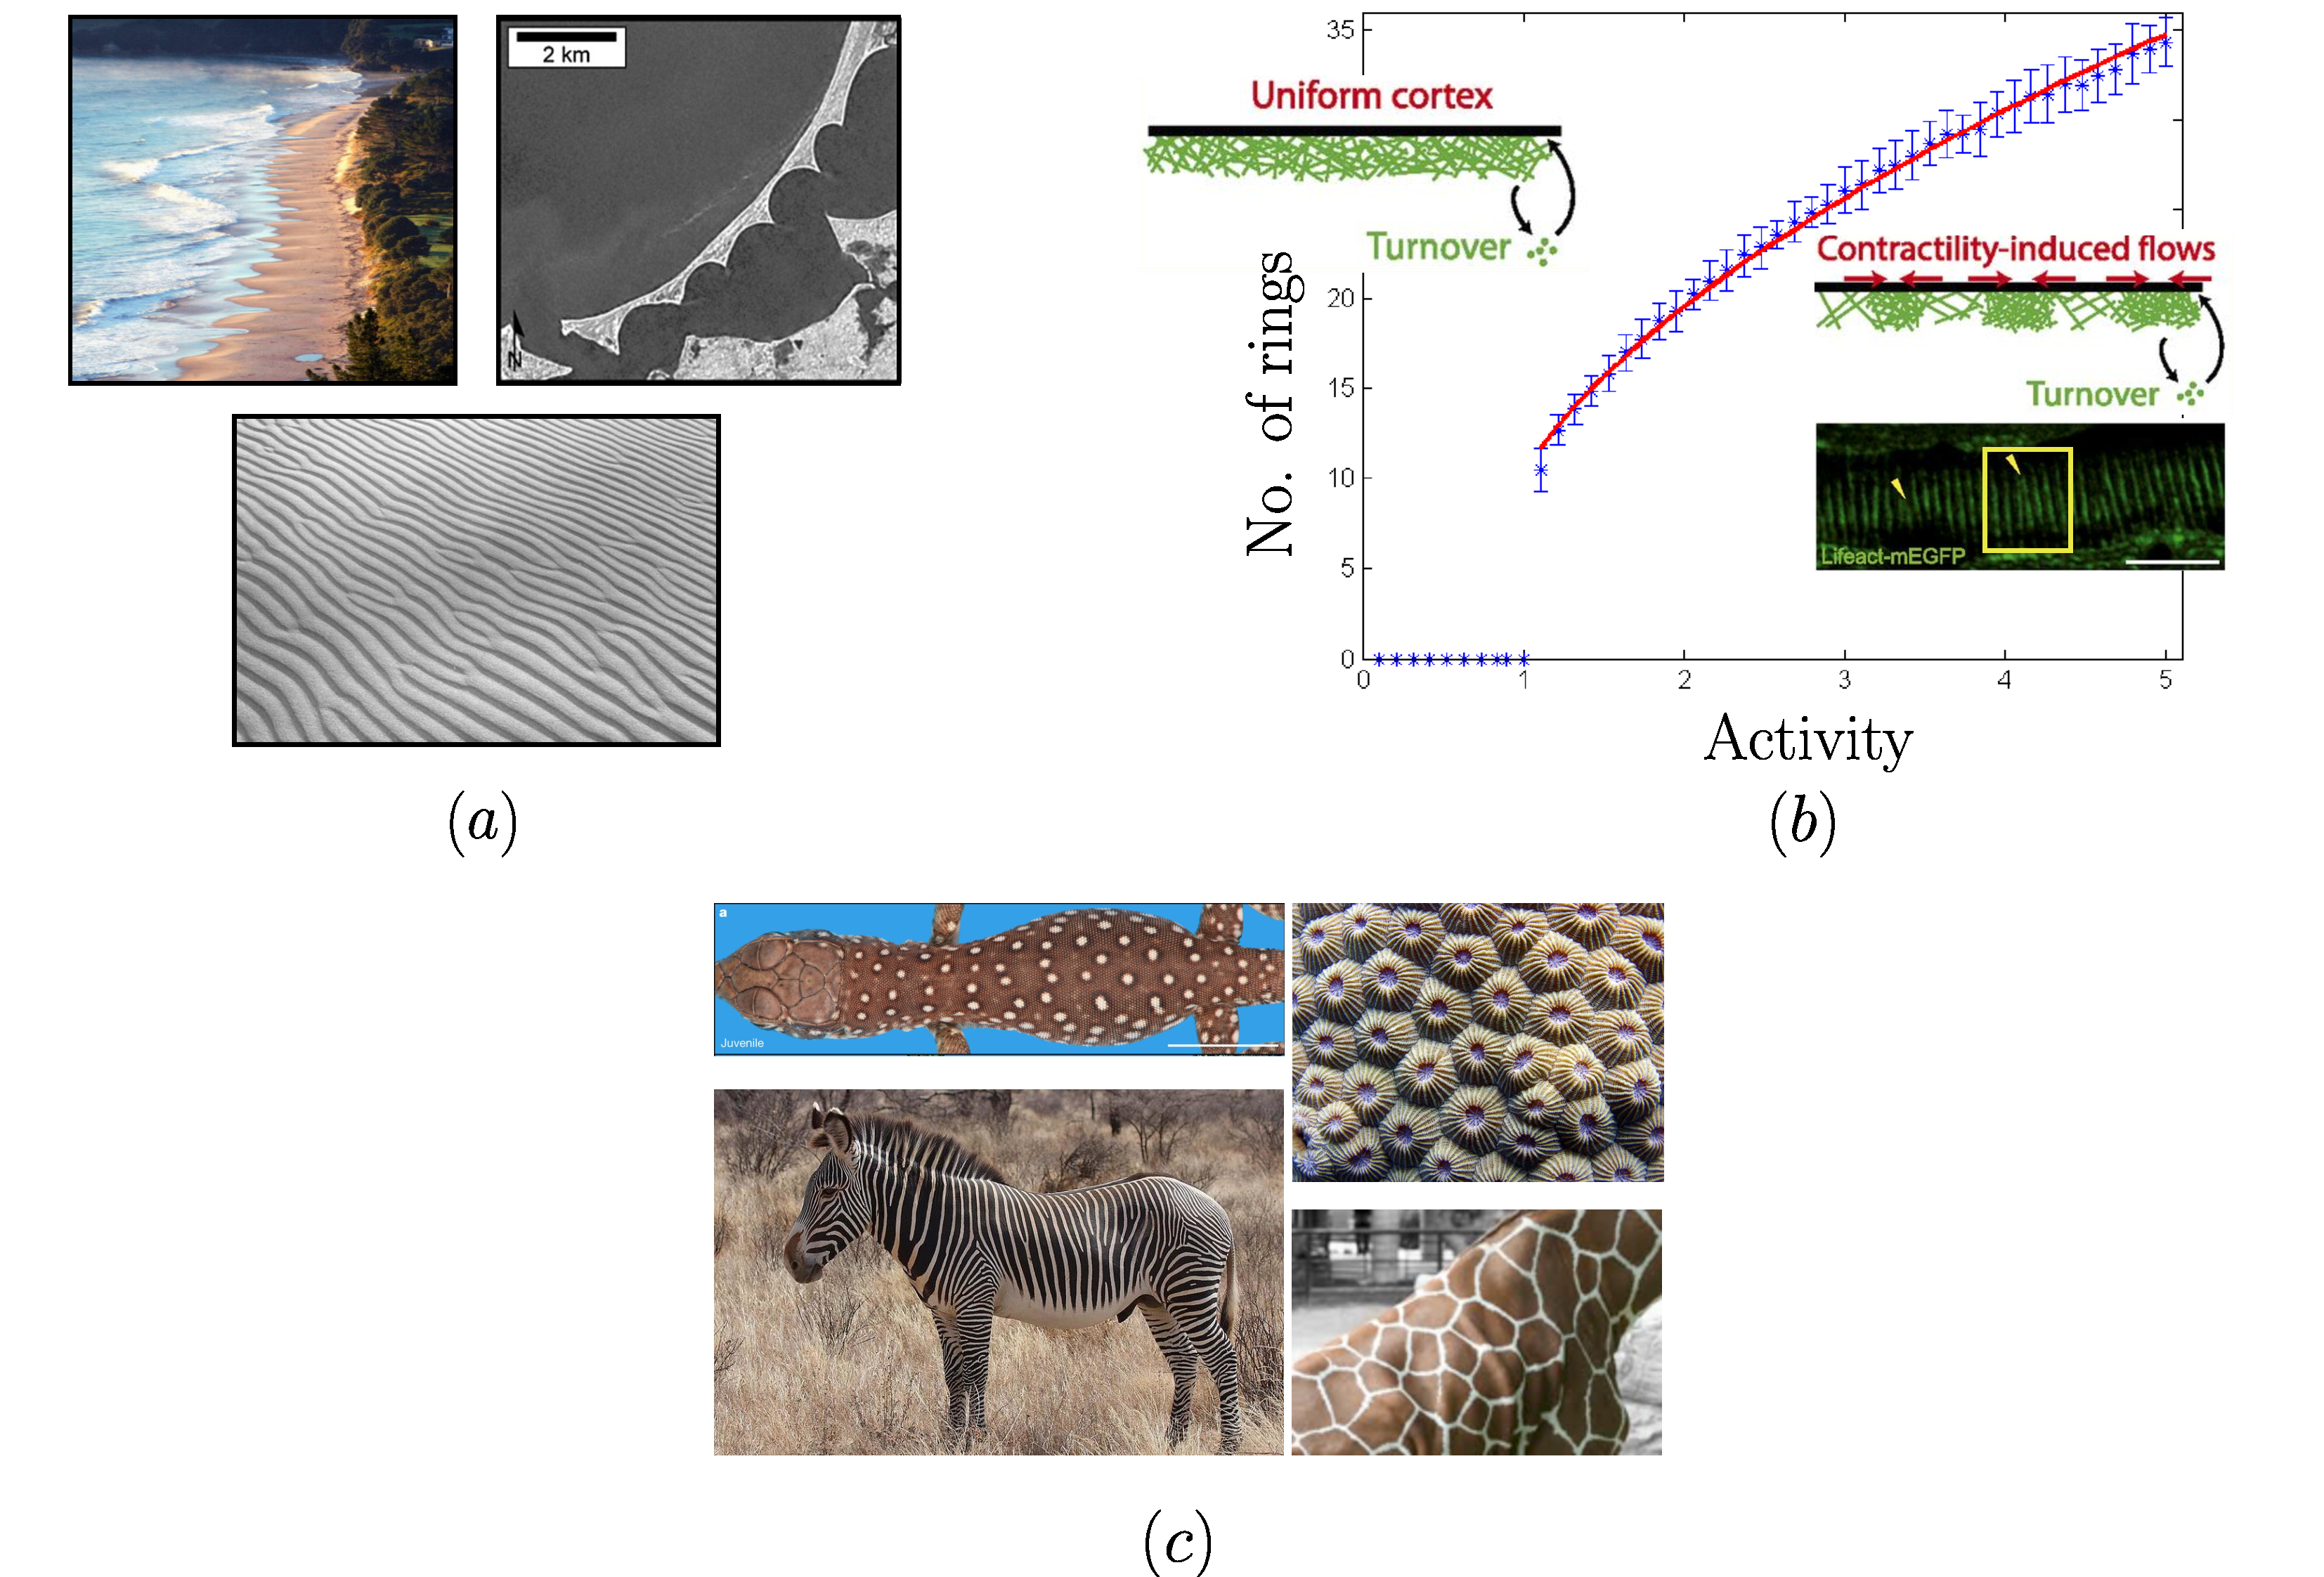
\includegraphics[width=\textwidth]{fig1.pdf}
		\caption{\label{fig_1_1} (a) Self-organization of wave-generated cusps on shorelines  \cite{coco2007} (top),  wind-generated  sand ripples \cite{anderson1990} (bottom).  (b)  Bifurcation diagram representing self-organization of supra-cellular actin rings above a threshold activity (reproduced from \cite{hannezo2015}). (c)  Skin patterns in animals can be explained by Turing instabilities based on an activator-inhibitor model \cite{turing1952}.}
\end{figure}

Self-organization is defined as a spontaneous formation of an organized structure at a global level through interaction between building blocks at the local level. This emergent behavior is an inherent characteristic of driven systems that exist far from thermodynamic equilibrium. %Systems are in thermodynamic equilibrium when there is no net flow of matter or energy, either within the system or in the surrounding. 
When a passive systems evolves towards its equilibrium state, entropy increases and energy is dissipated until equilibrium is reached, and then all fluxes are zero. By contrast, in  systems driven out-of-equilibrium through exchange of matter and/or energy with the surroundings, steady-states are possible with high entropy and sustained dissipation and fluxes \cite{chung2022,prigogine1963,nicolis1977}.  Energy input enables the self-organization into states with spatio-temporal order. Such self-organization in driven systems is ubiquitous across different scales, including the self-organization of ocean circulation \cite{Michael2017}, the formation of  coastlines and sand ripples under the action of waves and wind \cite{coco2007,anderson1990}, Fig.~\ref{fig_1_1}(a), or the active maintenance of membrane-less organelles by liquid-liquid phase separation within cells \cite{hyman2014}. Living systems are in general driven out-of-equilibrium by metabolism, and in particular through the transformation of chemical energy into mechanical work. This process that can be understood using the physical framework of \emph{active matter} \cite{marchetti2013}. To highlight the fundamental features of pattern formation in active matter, we describe next a minimal model for the actin cytoskeleton. Furthermore, this prototypical model provides a gentle introduction to actin dynamics and is a background for the new models proposed in this Thesis.

\section{The actin cytoskeleton and its active self organization}

The actin cytoskeleton is an inherently active  sub-cellular system consisting of a polymeric network of actin filaments and binding proteins. The continuous assembly and disassembly of this network, within turnover times of about 10s, and the binding/unbinding of cross-linkers and myosin motors consume energy from hydrolysis of ATP. As a consequence, the network behaves like an active viscoelastic fluid. Active gel theories are hydrodynamical models that have contributed to the understanding of how activity leads to emergent self-organization \cite{Prost:2015aa}. A mechanism by which active gels form out-of-equilibrium patterns is through self-reinforcing flows, during which a region of higher density of cytoskeletal material becomes locally more contractile, and hence generates a flow towards this region, which further reinforces the higher gel density and triggers a positive feedback loop. The interplay between gel viscosity, friction  with a substrate, turnover and diffusion of cytoskeletal components determines the critical activity for pattern formation and the typical spacing between foci of high density, Fig.~\ref{fig_1_1}(b). This conceptual framework has been mapped into a minimal 1D active gel model, which we describe next, and used to understand the assembly of actomyosin supra-cellular rings \cite{hannezo2015}.



In this model, balance of linear momentum in the gel is expressed along the  $x$  coordinate as
\begin{align}
	& \eta \frac{\partial^2 v}{\partial x^2} +   \frac{\partial \lambda(\rho)}{\partial x}   = \gamma  v,  \label{eq_1}
\end{align}
where the first term is the force density from viscous stresses with $\eta$ the gel viscosity and $v$ the velocity, the second is the force density from  the active contractile stress, which depends on density  $\rho$, and the last one is a frictional force density with coefficient $\gamma$.
This equation is coupled to a partial differential equation encoding mass conservation in the gel
\begin{align}
	& \frac{\partial \rho}{\partial t} + \frac{\partial (\rho v)}{\partial x}  -D \frac{\partial^2 \rho}{\partial x^2} - k(\rho-\rho_0)=0, \label{eq_2}
\end{align}
which states that local changes of gel density are caused by advective and diffusive transport, with diffusivity $D$, and by polymerization and depolymerization, where $k$ is the rate constant and $\rho_0$ the steady-state density for a uniform gel \cite{hannezo2015}. Linear stability of this model shows that beyond a critical activity, the uniform and quiescent steady state given by $v(x,t)=0$ and $\rho(x,t) = \rho_0$ becomes unstable and the system self-organizes into a dynamical steady state with foci of self-reinforcing flows.

We highlight next a number of features of this prototypical active gel model.\begin{enumerate}
	\item Nonlinearity. Nonlinearity makes it possible for the system to exhibit multiple solutions or to break symmetry. {In developmental biology, this nonlinearity provides resistance to perturbation or phenotypic robustness} \cite{green2017}. For instance, the self-assembly of supra-cellular rings described by Eqs.~(\ref{eq_1}) and~(\ref{eq_2}) results in high density regions, whose exponential densification as predicted by the linearized analysis is stabilized by nonlinearity.

	\item Bifurcation, i.e, a sudden change in qualitative behavior, number or/and stability of steady states, upon smooth variation in the model parameters.
	\item Pattern formation through a positive or negative feedback loop.
	The loss of stability of a uniform of high symmetry state is marked by symmetry breaking, leading to spatially inhomogenous patterns with a regular wavelength such as the actin foci predicted from Eqs.~(\ref{eq_1}) and~(\ref{eq_2}). These instabilities are driven by the self-reinforcing flows that result from a positive feedback between density and flow. This self-enhancing buildup of density is controlled by negative feedbacks between density and turnover and between density gradients and diffusion. Notable examples of self-organization from positive and negative feedback dynamics are hexagonal and stripy patterns appearing in the skin of animals Fig.~\ref{fig_1_1}(c), which  can be  described by the system of reaction-diffusion equations put forth by  \citet{turing1952}. The simplest Turing model that supports patterning comprises two species  $u$ and $v$, governed by
	\begin{align}
		& \frac{\partial u}{\partial t} =f(u,v) +D_u \frac{\partial^2 u}{\partial x^2},  \\ &
		\frac{\partial v}{\partial t}=g(u)  - k_v v + D_v \frac{\partial^2 v}{\partial x^2}.  \nonumber
	\end{align}
	Species $u$ promotes the production of  substance $u$ as well as substance $v$ through functions $f$ and $g$. However, substance $v$ inhibits the production of both substance $v$ and $u$ due to self-inhibition through $k_v$ and function $f$. Classic Turing instabilities appear when the ratio $D_v/D_u$ of the two diffusion constants increases beyond a threshold. This condition breaks the stability of a uniform state and spontaneously bifurcates to alternating  waves of concentration differences for $u$. Here, the feedback loops provide the generic mechanism for self-organization. Positive feedback through functions $f$ and $g$ leads to the amplification of perturbations and negative feedback triggers a response that controls the growth of a perturbation.
\end{enumerate}

\section{Self-organization of sub-cellular cytoskeletal networks}

Biological structures across length-scales, from the molecular to the organ level, adopt their shape and composition through the self-organization of patterns \cite{isaeva2012,sekimura2013}, which need to balance robustness and adaptability. Focusing on cytoskeletal networks, in this section we review the organization of actin filament networks at sub-cellular scales, and how reconstituted systems recapitulate these network architectures suggesting a central role of self-organization. We also briefly discuss self-organization in microtubule and intermediate filament networks.


\subsection{The actin cytoskeleton}

The actin cytoskeleton is a crosslinked and dynamical network of actin filaments. It is composed of more than $100$ structural and regulatory proteins  \cite{kelkar2020, chugh2018, thomas2012} such as myosin-II, fascins, $\alpha$-actinin, ADF/cofilin, and profilin. This network is inherently out-of-equilibrium, i.e.~exposed to a continuous flux of energy from  Adenosine triphosphate (ATP) hydrolysis. As a consequence, actin-binding proteins such as myosin-II, fascins or $\alpha$-actinin attach to actin filaments, possibly slide along them, and exert contractile stress through complementary microscopic mechanisms \cite{murrell2015, lenz2012, koenderink2018}. Moreover, proteins such as ADF/cofilins and profilin actively regulate actin filament disassembly  and polymerization \cite{rosenblatt1997, murrell2015,krishnan2009}, and hence, even if these processes balance, the resulting steady-state is highly out-of-equilibrium. From a mechanical standpoint, the actin cytoskeleton exhibits a diversity of behaviors. Depending on the relative importance of different active molecular mechanisms within the network and its architecture, actin gels can either push by polymerization-induced forces or pull by contractile forces induced by myosin motors, cross-linkers or depolymerization. Depending on the rate of deformation compared to the turnover timescale of its constituents, it can either store elastic energy or dissipate it like a fluid \cite{kollmannsberger2011}.

This complex interplay of molecular, biochemical and mechanical processes allows the cortical network to self-organize into a variety of architectures, each  playing different biological roles. Because actin filaments are polar, these network architectures can be classified depending on their orientational order as reviewed next.


\subsubsection{Isotropic actin networks}

In  suspended cells, on a soft substrate or in membrane blebs, the actin cortex adopts an isotropic and relatively sparse architecture \cite{morone2006, svitkina2020}, Fig.~\ref{chap_1_fig_1}(a). The isotropy of the network can be explained by several mechanisms including thermal vibrations that tend to randomize the network \cite{salbreux2009,anne2016}, actin turnover and severing tending to destabilize any degree of anisotropy in the network, and actin polymerization lacking any preferential orientation \cite{svitkina2020}. In cells spread on stiff surfaces, isotropic actin networks coexist  with other architectures described below. The isotropic architecture leads to isotropic network tension, which contributes to cell rounding at the onset of mitosis \cite{salbreux2012, kelkar2020}.


\begin{figure}
	\centering
	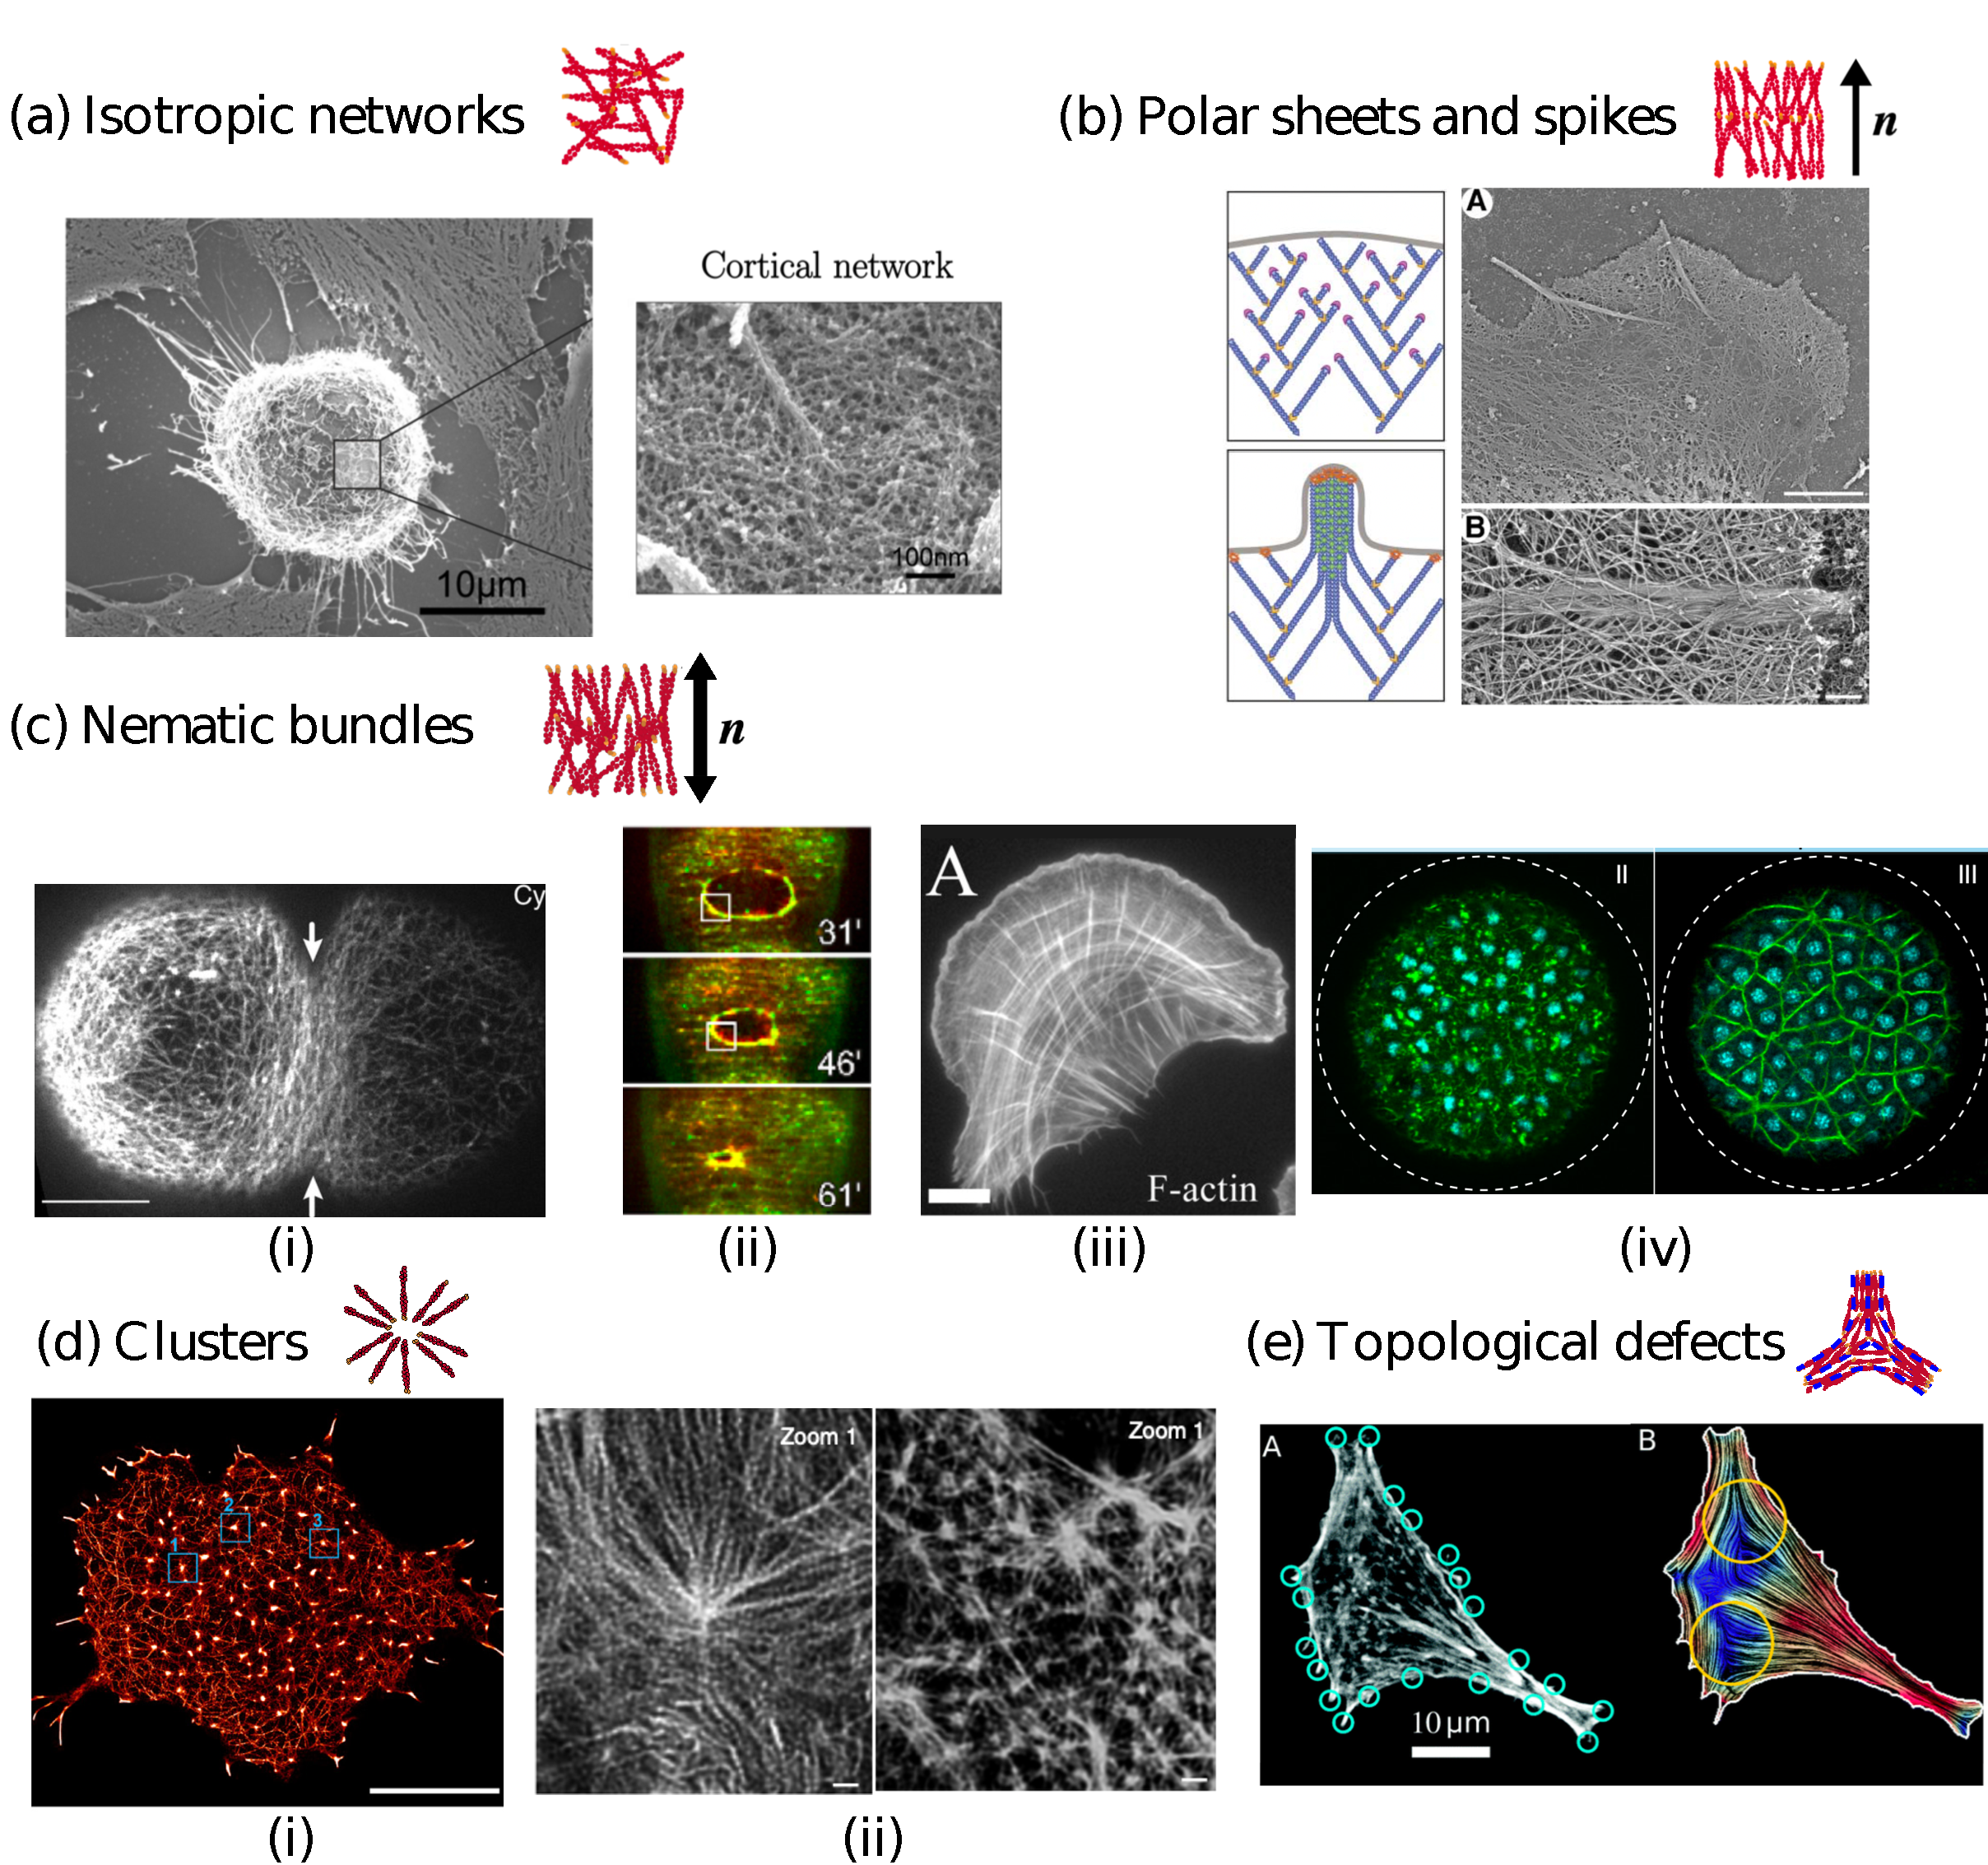
\includegraphics[width=0.98\textwidth]{fig2.pdf}
	\caption{\label{chap_1_fig_1} Diverse architectures in the actin cytoskeleton. (a) Isotropic network in the actin cortex of a spherical cell \cite{kelkar2020}. (b) Polar sheets (lamellipodia) and spikes (fillipodia) at the edge of an adherent cell \cite{Mejillano:2004wx}. (c)  Nematic actin bundles (i) during cytokinesis \cite{anne2016}, (ii) during supra-cellular wound healing \cite{10.1242/jcs.109066}, (iii) forming patterns of stress fibers in adherent cells \cite{hotulainen2006}, or (iv) during actomyosin-dependent cellularization \cite{dudin2019}. (d) Actin clusters with star or aster architecture reproduced from  \cite{xia2019} in (i) and from \cite{fritzsche2017} in (ii).% (ii) reconstituted systems \cite{murrell2012} and (iii) tactoids in a reconstituted system \cite{weirich2019}.  
	(e) Topological defects of actin orientation in an adherent cell \cite{schakenraad2020}. }
\end{figure}

\subsubsection{Polar sheets and spikes}

Adherent cells often exhibit at their edge a branched actin network sheet called lamellipodium. Spike-like protrusions of bundled actin filaments such as filopodia are also common at cell edges. These sheets and spikes are polar, Fig.~\ref{chap_1_fig_1}(b), with  plus ends pointing towards the cell edge, push on the plasma membrane thanks to polymerization-induced forces, and enable cells to migrate and probe their environment. Filopodia grow depending on actin polymerases  VASP and formins \cite{svitkina2003} and are rich in crosslinkers \cite{bartles2000}, whereas actin polymerization in lamellipodia is primarily controlled by Arp2/3. Filopodia and lamellipodia are devoid of myosin-II and hence are non-contractile \cite{nemethova2008}. The lamellipodium progressively looses its polarity as the network moves backward in the cell during retrograde flow \cite{svitkina2020}. Likewise, polar filopodial bundles are recycled into nematic contractile bundles, reviewed next, during retrograde flow \cite{nemethova2008,doi:10.1091/mbc.e08-01-0034}.


\subsubsection{Nematic actin bundles}

Nematic actin bundles are dense elongated structures where actin filaments are aligned along their axis in a bipolar configuration, i.e.~on average there is an equal number of filaments pointing with plus and minus ends in either direction along the axis. These structures assemble in a variety of cellular contexts, including cytokinesis \cite{anne2016}, wound healing at sub-cellular 
\cite{mandato2001} and supra-cellular scales \cite{10.1242/jcs.109066}, stress fibers \cite{hotulainen2006}, or during actomyosin-dependent cellularization \cite{dudin2019}, Fig.~\ref{chap_1_fig_1}(c). 

Actin binding proteins such as $\alpha$-actinin  and myosin-II contribute to the tight packing of actin filaments into nematic bundles \cite{blanchoin2014,winkelman2016,lehtimaki2021, laporte2012}. As bundles emerge,  crosslinkers may bind at a higher rate due to favorable filament orientation  \cite{courson2010}. Additionally, the presence  and amount of crosslinkers slows down turnover \cite{SCHMOLLER2011350}  stabilizing dense and cross-linked actin structures. The higher density allows more cross-linkers to bind to the network,  further stabilizing the bundle architecture through positive feedback. The higher cytoskeletal density in nematic bundles and the increased ability of myosin-II to contract an aligned network leads to high, localized and anisotropic active tension \cite{bergert2015, turlier2014, mayer2010, kelkar2020}. Moreover, binding proteins may locally enhance  orientational order of the actin network  \cite{lehtimaki2021}, which in turn also enhances  contractility \cite{kelkar2020}. Thus, the local orientation of the actin filaments in the network is a major determinant of its active mechanical properties. In rounded cells, a tension inhomogeneity  can lead to the self-organization of a contractile  ring, which divides a cell \cite{greenspan1978, mietke2019_2, mietke2019, koyama2012,gladilin2015,biron2005,turlier2014,sain2015,zhao2016,akkacs1980,poirier2012} or heals a wound in an egg cell \cite{mandato2001}.


\begin{figure}
	\centering
	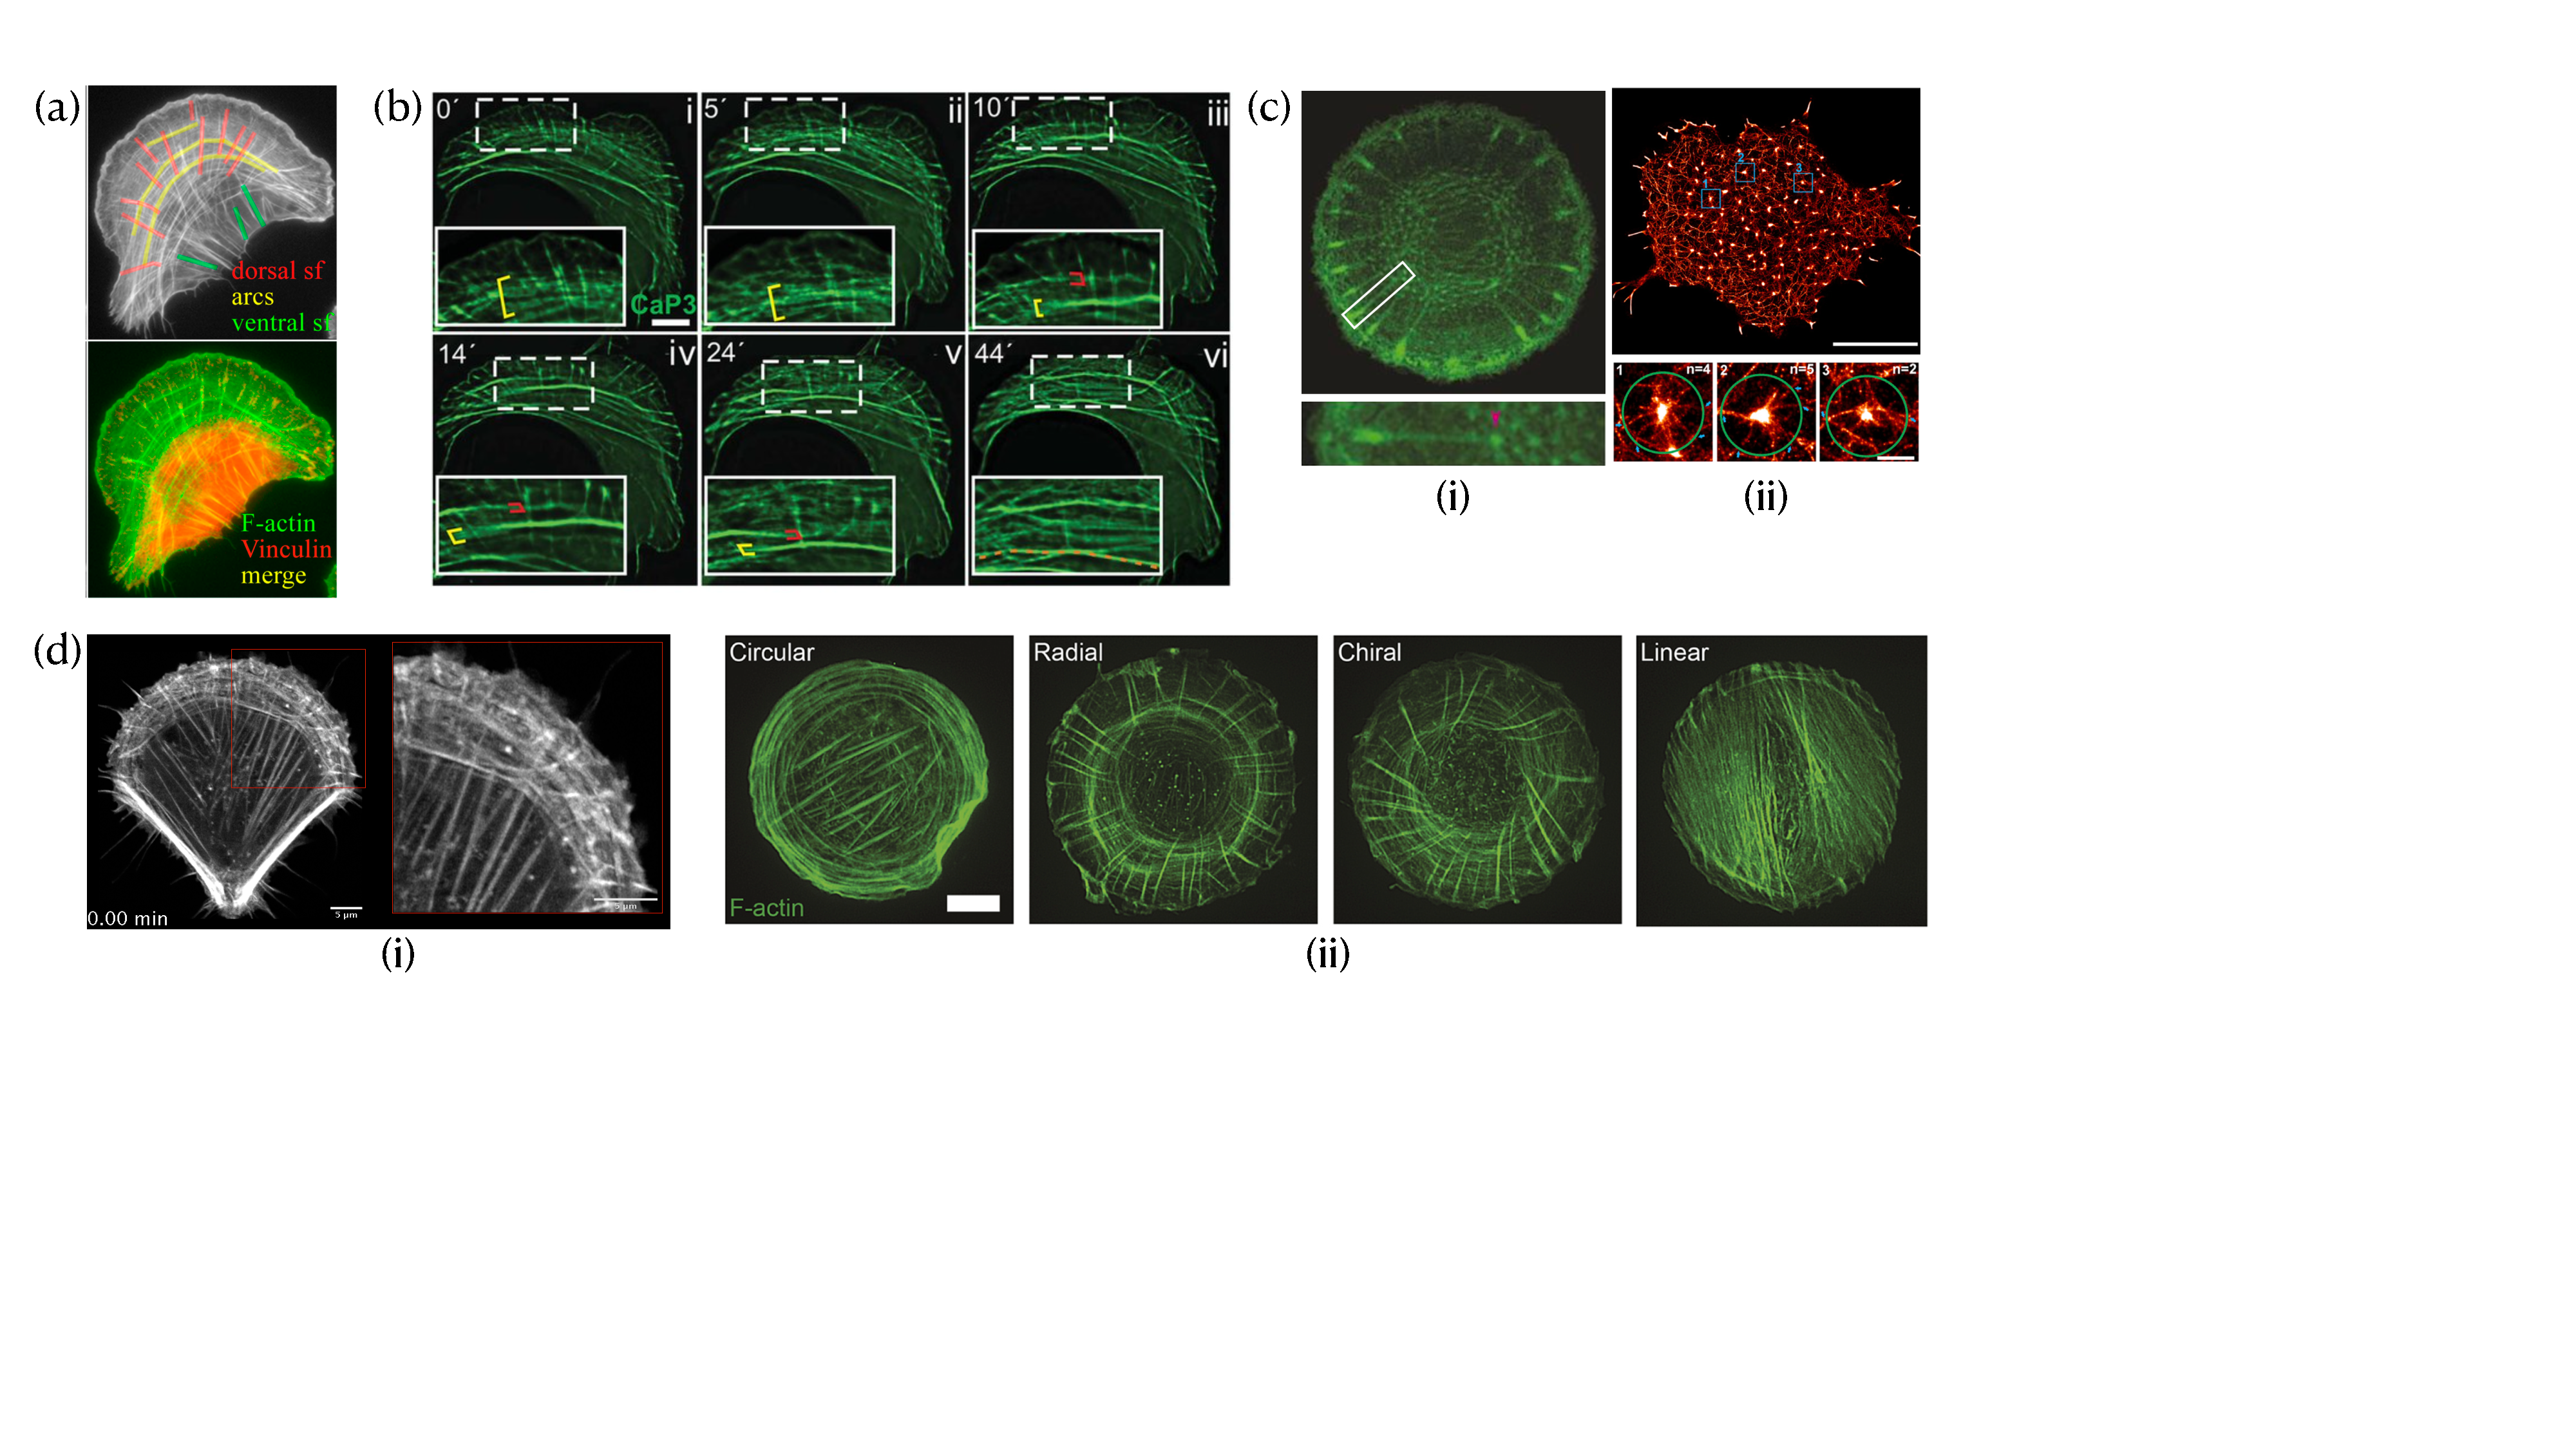
\includegraphics[width=0.98\textwidth]{fig22.pdf}
	\caption{\label{chap_1_fig_22} Dense nematic actin bundles in adherent cells. (a) Families of stress fibers and association to adhesion complexes \cite{hotulainen2006}. (b) Dynamical reconfigurations of stress fibers near the leading edge \cite{tojkander2015}. (c) Coexistence of nematic bundles and asters. Images taken from  \cite{jalal2019} in (i) and  from \cite{xia2019} in (ii). (d) Geometrically regular organization of stress fibers through adhesion patterning in (i) polar \cite{10.1242/jcs.236604} and (ii) circular \cite{jalal2019} geometries. }
\end{figure}



When placed on a stiff substrate, rounded cells break symmetry as they spread \cite{gupta2015, rens2020,callan2008}.
In such spread cells, contractile actin bundles emerge and often form patterns with regular spacing \cite{jalal2019}. These fibers often interact with the extracellular matrix through mechanosensitive focal adhesions, Fig.~\ref{chap_1_fig_22}(a), which transmit tractions to the extracellular matrix \cite{tojkander2012,livne2016}, thereby enabling spreading and migration. Based on their sub-cellular localization and interactions
with extracellular matrix, nematic bundles of adherent cells are  classified into three families \cite{lehtimaki2021, tee2015, tojkander2015,wirshing2017, yolland2019, jalal2019}, Fig.~\ref{chap_1_fig_22}(a). (i) Dorsal stress fibers are attached to the substrate via focal adhesions and are oriented in a radial direction towards the nucleus. Formins mediate the formation of these fibers, which are devoid of myosin and $\alpha$-actinin, and are thought to be non-contractile \cite{lehtimaki2021}. (ii) Transverse stress fibers are oriented along the cell edge and perpendicular to dorsal fibers. They are not connected to the extracellular matrix via focal adhesions and are decorated with both $\alpha$-actinin and myosin. (iii) Ventral stress fibers are generated through the coalescence of pre-existing radial and transverse stress fibers, are contractile,  and are connected to focal adhesions at both ends.

Stress fibers are highly dynamical, with frequent nucleation and fusion events near the leading edge, Fig.~\ref{chap_1_fig_22}(b). Ventral stress fibers assemble through a fusion of radial and transverse arches. However, the mechanism leading to the formation of dorsal and transverse fibers is still an open question. It is unclear to what degree stress fibers emerge from the recycling of pre-existing structures, such as filopodia \cite{nemethova2008,doi:10.1091/mbc.e08-01-0034} or focal adhesions, or assemble de novo. Observations in cells,  reconstituted systems and simulations suggest that stress fibers can assemble from the actin cortex without the involvement of stress fiber precursors or actin polymerization at focal adhesions \cite{lehtimaki2021,livne2016,deshpande2015,freedman2018}. In the absence of anchorage sites, straight actomyosin bundles have been observed to self-organize and dynamically fuse with adjacent bundles \cite{lehtimaki2021,livne2016,wirshing2017}. Furthermore, these bundles coexist in a mechanical continuum with a sparse and isotropic actin network  \cite{vignaud2021}. They can also coexist with actin asters to form networks of nematic bundles connecting dense clusters \cite{jalal2019,xia2019}, Fig.~\ref{chap_1_fig_22}(c). By controlling the shape of adhesive cells through adhesion patterning, stress fibers adopt remarkably regular arrangements that depend on cell shape, size, substrate stiffness and degree of maturation \cite{10.1242/jcs.236604,jalal2019}, Fig.~\ref{chap_1_fig_22}(d). 


\subsubsection{Actin clusters}

Actin networks can also form patterns of high-density foci surrounded by convergent filaments in so-called \emph{asters}, \emph{stars} or \emph{foci} \cite{nishikawa2017,xia2019,fritzsche2017}, see Fig.~\ref{chap_1_fig_1}(d). Such high-density punctuated structures naturally emerge in discrete network simulations of the actin cytoskeleton, which establish their emergence and morphology  depending on model parameters such as filament bending rigidity and length,  concentration of motors and crosslinkers, and actin turnover \cite{freedman2018,li2017,yu2018,mak2016, hiraiwa2016, miller2018}. An interplay between  Arp2/3, formin, and capping proteins has also been shown control cluster patterning \cite{xia2019}. Asters can be polarity sorted or have mixed polarity. Simulations predict mixed-polarity asters at intermediate myosin concentration and high cross-linker concentration \cite{freedman2018}, consistent with mixed polarity asters in cells with low myosin-II expression \cite{xia2019}. Actin clusters can be stable  or short-lived \cite{hiraiwa2016,mcfadden2017}. The short lifetime of asters is attributed to fast turnover, de-branching, or filament severing \cite{yu2018,li2017,mak2016}. As mentioned above, nematic bundles can converge into actin clusters to form complex actin organizations, Fig.~\ref{chap_1_fig_22}(c).

\subsubsection{Topological defects}

Orientational order can smoothly vary or develop orientational  \emph{defects}. In nematic systems, these defects have either half-integer charge such as comet-like ($+1/2$) or trefoil-like ($-1/2$), or full-integer charge such as $+1$ spiral-like or $+1$ aster-like defects.  Activity renders $+1/2$ defects motile along their axis of symmetry, whereas due to their three-fold symmetry,  $-1/2$ defects do not propel \cite{thijssen2020,vafa2020}. Topological defects in stress fiber organization have been reported in adherent single cells  \cite{schakenraad2020},  Fig.~\ref{chap_1_fig_1}(e).


\subsubsection{Interplay between actin architectures cellular shape}

Each actomyosin architecture correlates with distinct cell shape deformations. Polar actin bundles form narrow protrusions such as filopodia at the cell periphery, whereas lamellipodial polar networks form sheets \cite{blanchoin2014}. Equatorial actin nematic bundles constrict  dividing cells in the cytokinetic furrow \cite{anne2016}. Nematic defects  facilitate the reorganization of stress fibers supporting cellular shape changes \cite{schakenraad2020}. The role of actin clusters in cell shape deformation has not been systematically analyzed. A more comprehensive review of shape changes driven by nematic architectures is provided in Chapter~\ref{chap_6}.



\subsubsection{Recapitulation of actin architectures in reconstituted systems}

Supporting the idea of self-organization in the actin cytoskeleton, in vitro reconstituted systems mixing actin filaments with cross-linkers or myosin-II motors in different conditions have recapitulated actin architectures observed in cells. Actin filaments and bundling agents alone can produce remarkably regular networks of dense actin bundles  \cite{huber20152}, Fig.~\ref{chap_1_fig_222}(a). Addition of myosin-II motors to actin gels can lead to regular patterns of asters connected by bundles \cite{murrell2012,seara2018}, Fig.~\ref{chap_1_fig_222}(b), or to gels populated by motile nematic half-integer defects \cite{kumar2018,seara2018}, Fig.~\ref{chap_1_fig_222}(c). In a different regime, a suspension of actin filaments and crosslinkers organizes into spindle-shaped clusters of high density and alignment called tactoids \cite{weirich2017}, which can deform and split upon the action of myosin-II \cite{weirich2019}, Fig.~\ref{chap_1_fig_222}(d). By patterning actin polymerization, constricting actomyosin rings have been reconstituted in vitro  \cite{Ennomani2016}, Fig.~\ref{chap_1_fig_222}(e). Finally, cross-linking of actin filaments confined to a lipid vesicle self-organize into bundled rings, which upon addition of myosin-II become contractile and deform the vesicle \cite{bashirzadeh2022, litschel2021}, Fig.~\ref{chap_1_fig_222}(f).


\subsubsection{Actin bundles as templates during development}

Besides their intrinsic functionality, the ability of actin networks to develop patterns of dense bundles can serve as templates during morphogenesis of other structures. One instance is the formation of ridges in butterfly wing scales, which control their optical properties, \cite{DINWIDDIE2014404} and Fig.~\ref{chap_1_fig_777}(a). Mature scales result from the cuticle of dead cells. During development in the wing epithelium, an actin pre-pattern consisting of parallel dense bundle along elongated cellular extensions develops on an homogeneous cell surface, which then guides cuticle deposition and patterning, and is finally disassembled leaving cuticle ridges behind, Fig.~\ref{chap_1_fig_777}(b). Hence, actin patterning plays a guiding role during morphogenesis, but the final functional structure does not contain actin.   

Another remarkable pattern formed by dense and elongated actin structures are the so-called actin microridges. Microridges form in the apical surfaces of mucosal epithelial cells, as shown for scale epidermal cells in different fish species in Fig.~\ref{chap_1_fig_777}(c) \cite{https://doi.org/10.1002/ar.23965}. These maze-like structures form from point-like actin foci, which elongate, reorganize Fig.~\ref{chap_1_fig_777}(d), and eventually protrude out of the apical plane. Their development and maturation is complex, not fully understood and involves myosin contractility, actin crosslinking, and arp2/3 polymerization. The identification of dense actin bundles below the protrusions \cite{BEREITERHAHN1979316} suggests that microridges protrude by a branched network polymerized by arp2/3 out of a pre-pattern of dense nematic bundles organized from the initially isotropic and uniform apical cortex. The initial stages of microridge formation are highly dynamical and can be guided by mechanical cues such as cell stretching, Fig.~\ref{chap_1_fig_777}(d) \cite{10.1083/jcb.201904144}. Although the function of actin microridges remains open, recent work suggests a role as a pre-pattern and structural anchoring for motile cilia \cite{Yasunaga:2022uh}. 


\begin{figure}
	\centering
	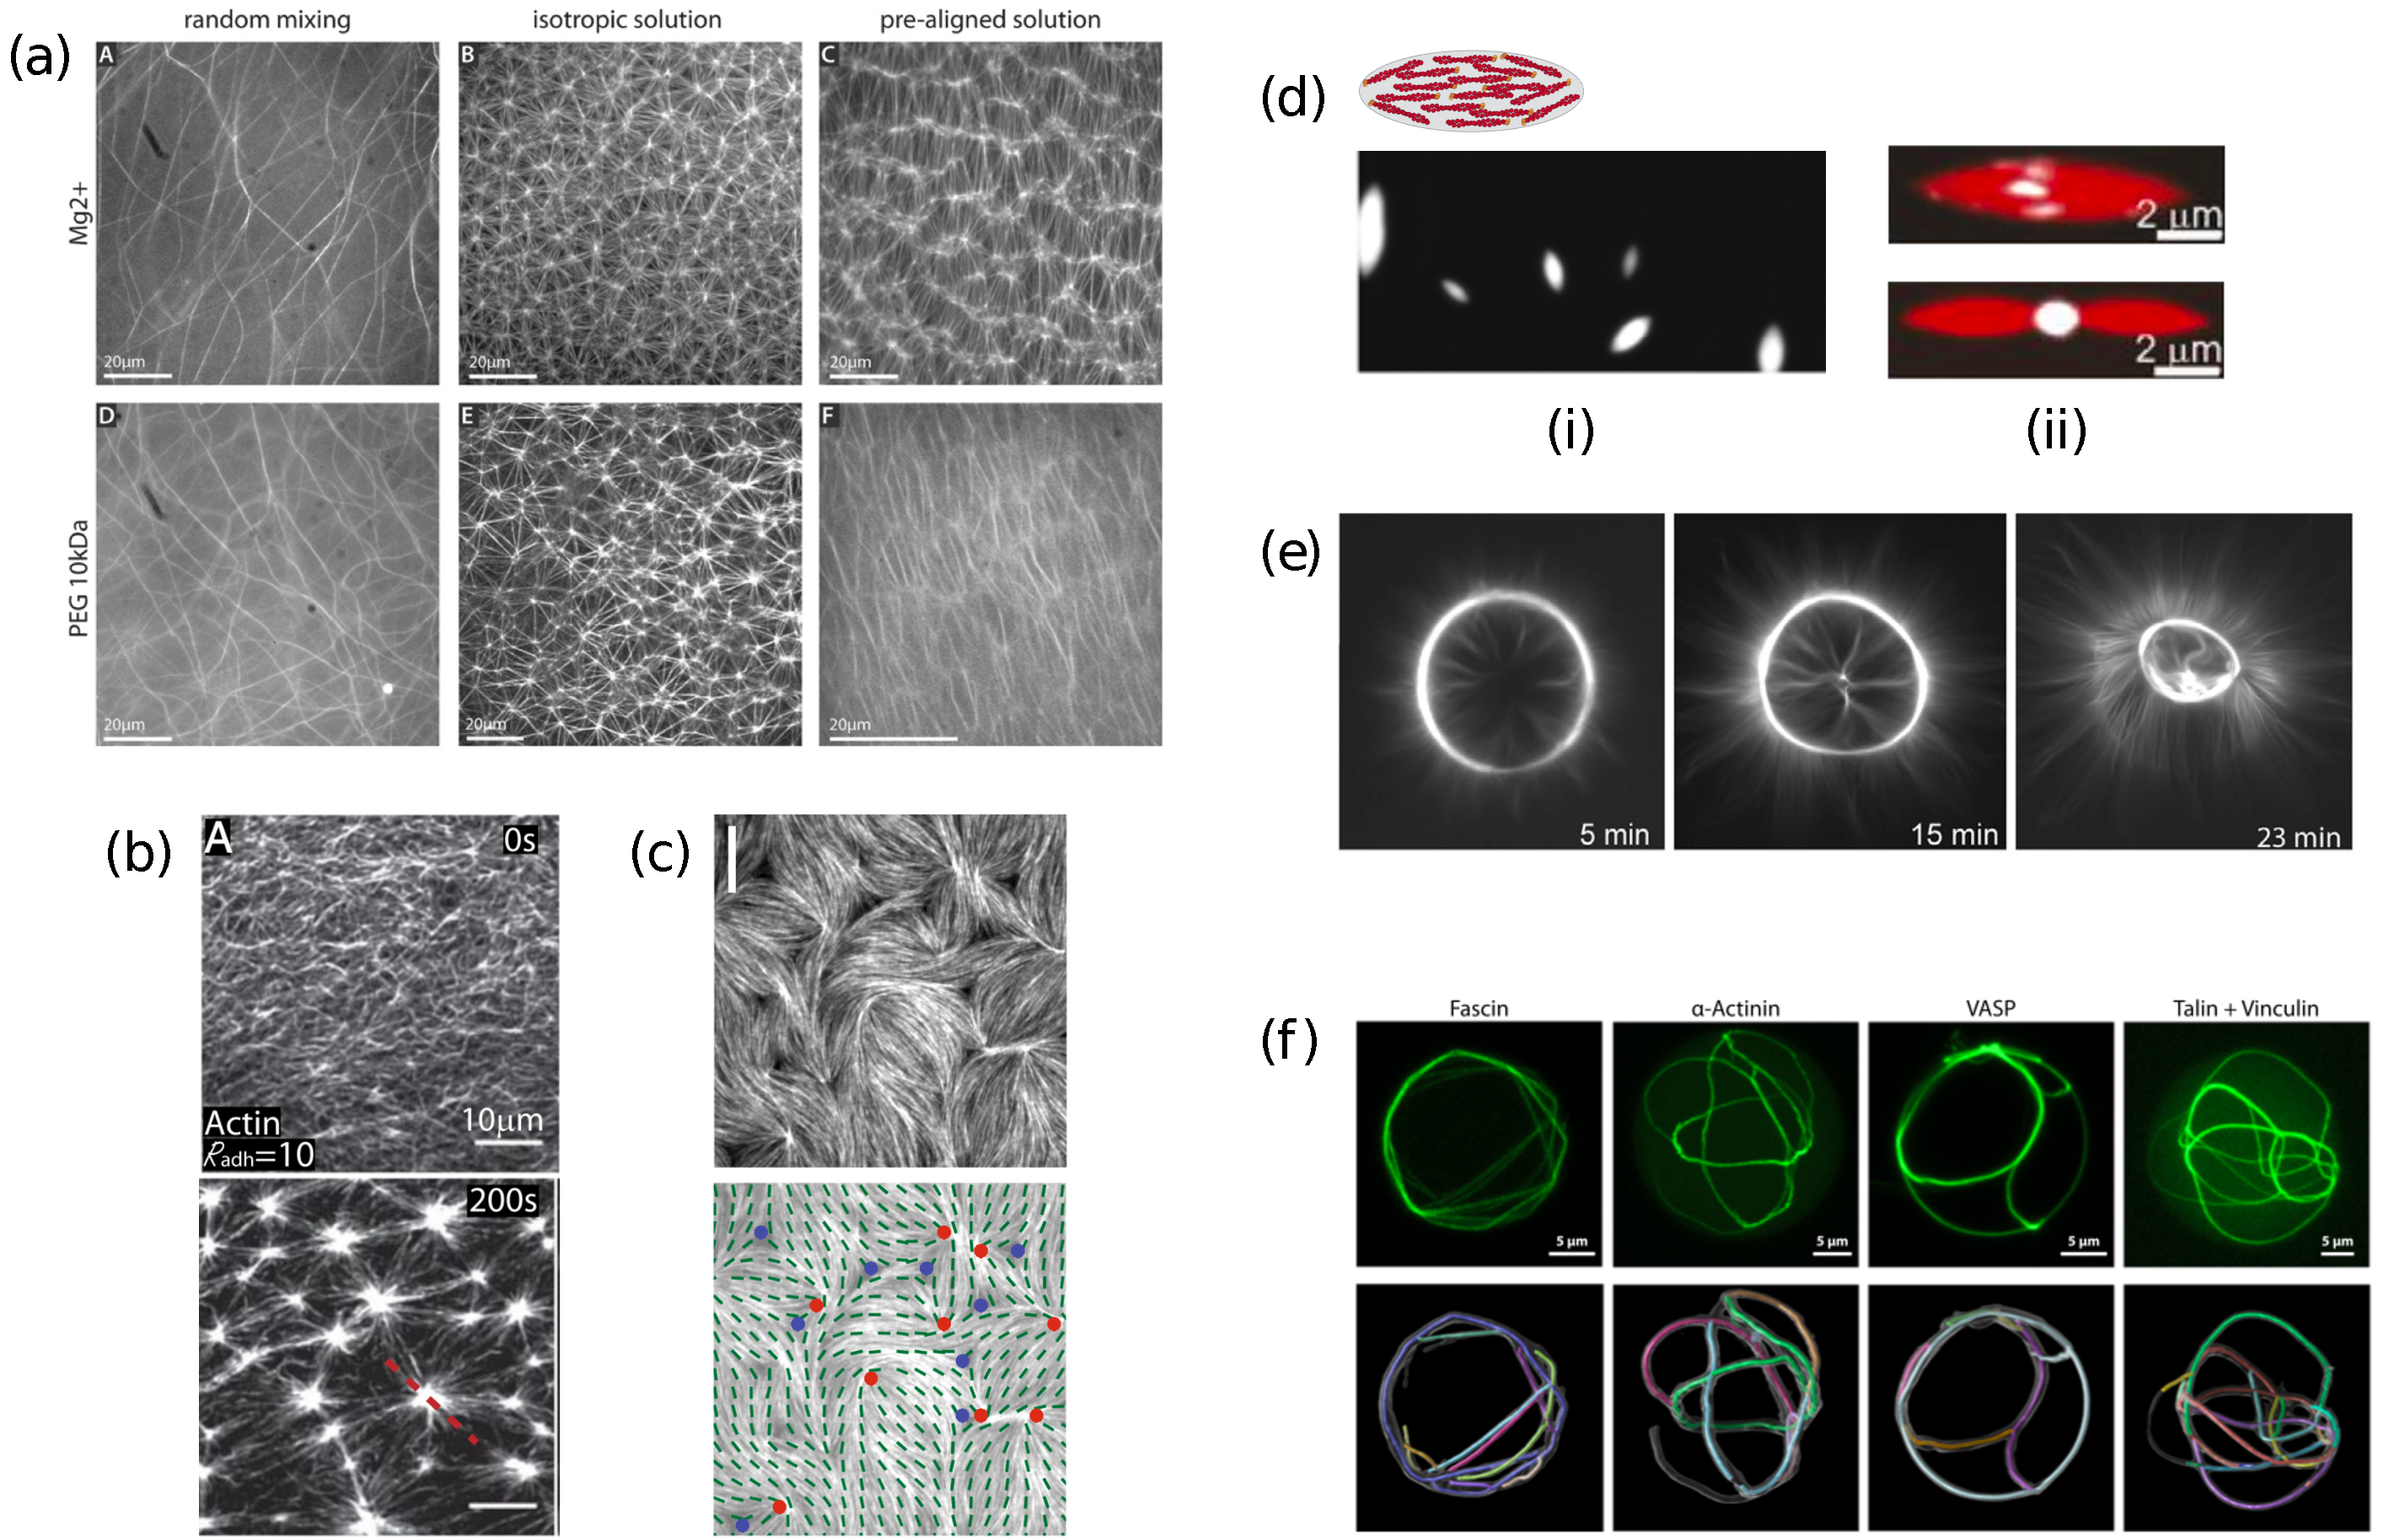
\includegraphics[width=0.99\textwidth]{fig222.pdf}
	\caption{\label{chap_1_fig_222} Architectures in reconstituted actin gels. (a) Diversity of regular network organizations in actin filament preparations upon unspecific bundling by crowding agents \cite{huber20152}. (b) Aster and bundle formation in cross-linked actin gels following addition of myosin-II \cite{murrell2012}. (c) Motile nematic defects in actomyosin gels \cite{seara2018}. (d) Formation of tactoids (nematic actin droplets) in (i) cross-linked actin gels \cite{weirich2017}, and (ii) deformation of tactoids by myosin-II activity \cite{weirich2019}. (e) Reconstituted contractile actomyosin ring \cite{Ennomani2016}. (f) Reconstituted actin rings on lipid vesicles with different cross-linkers, which can become contractile upon addition of myosin-II  \cite{litschel2021}.}
\end{figure}


\begin{figure}
	\centering
	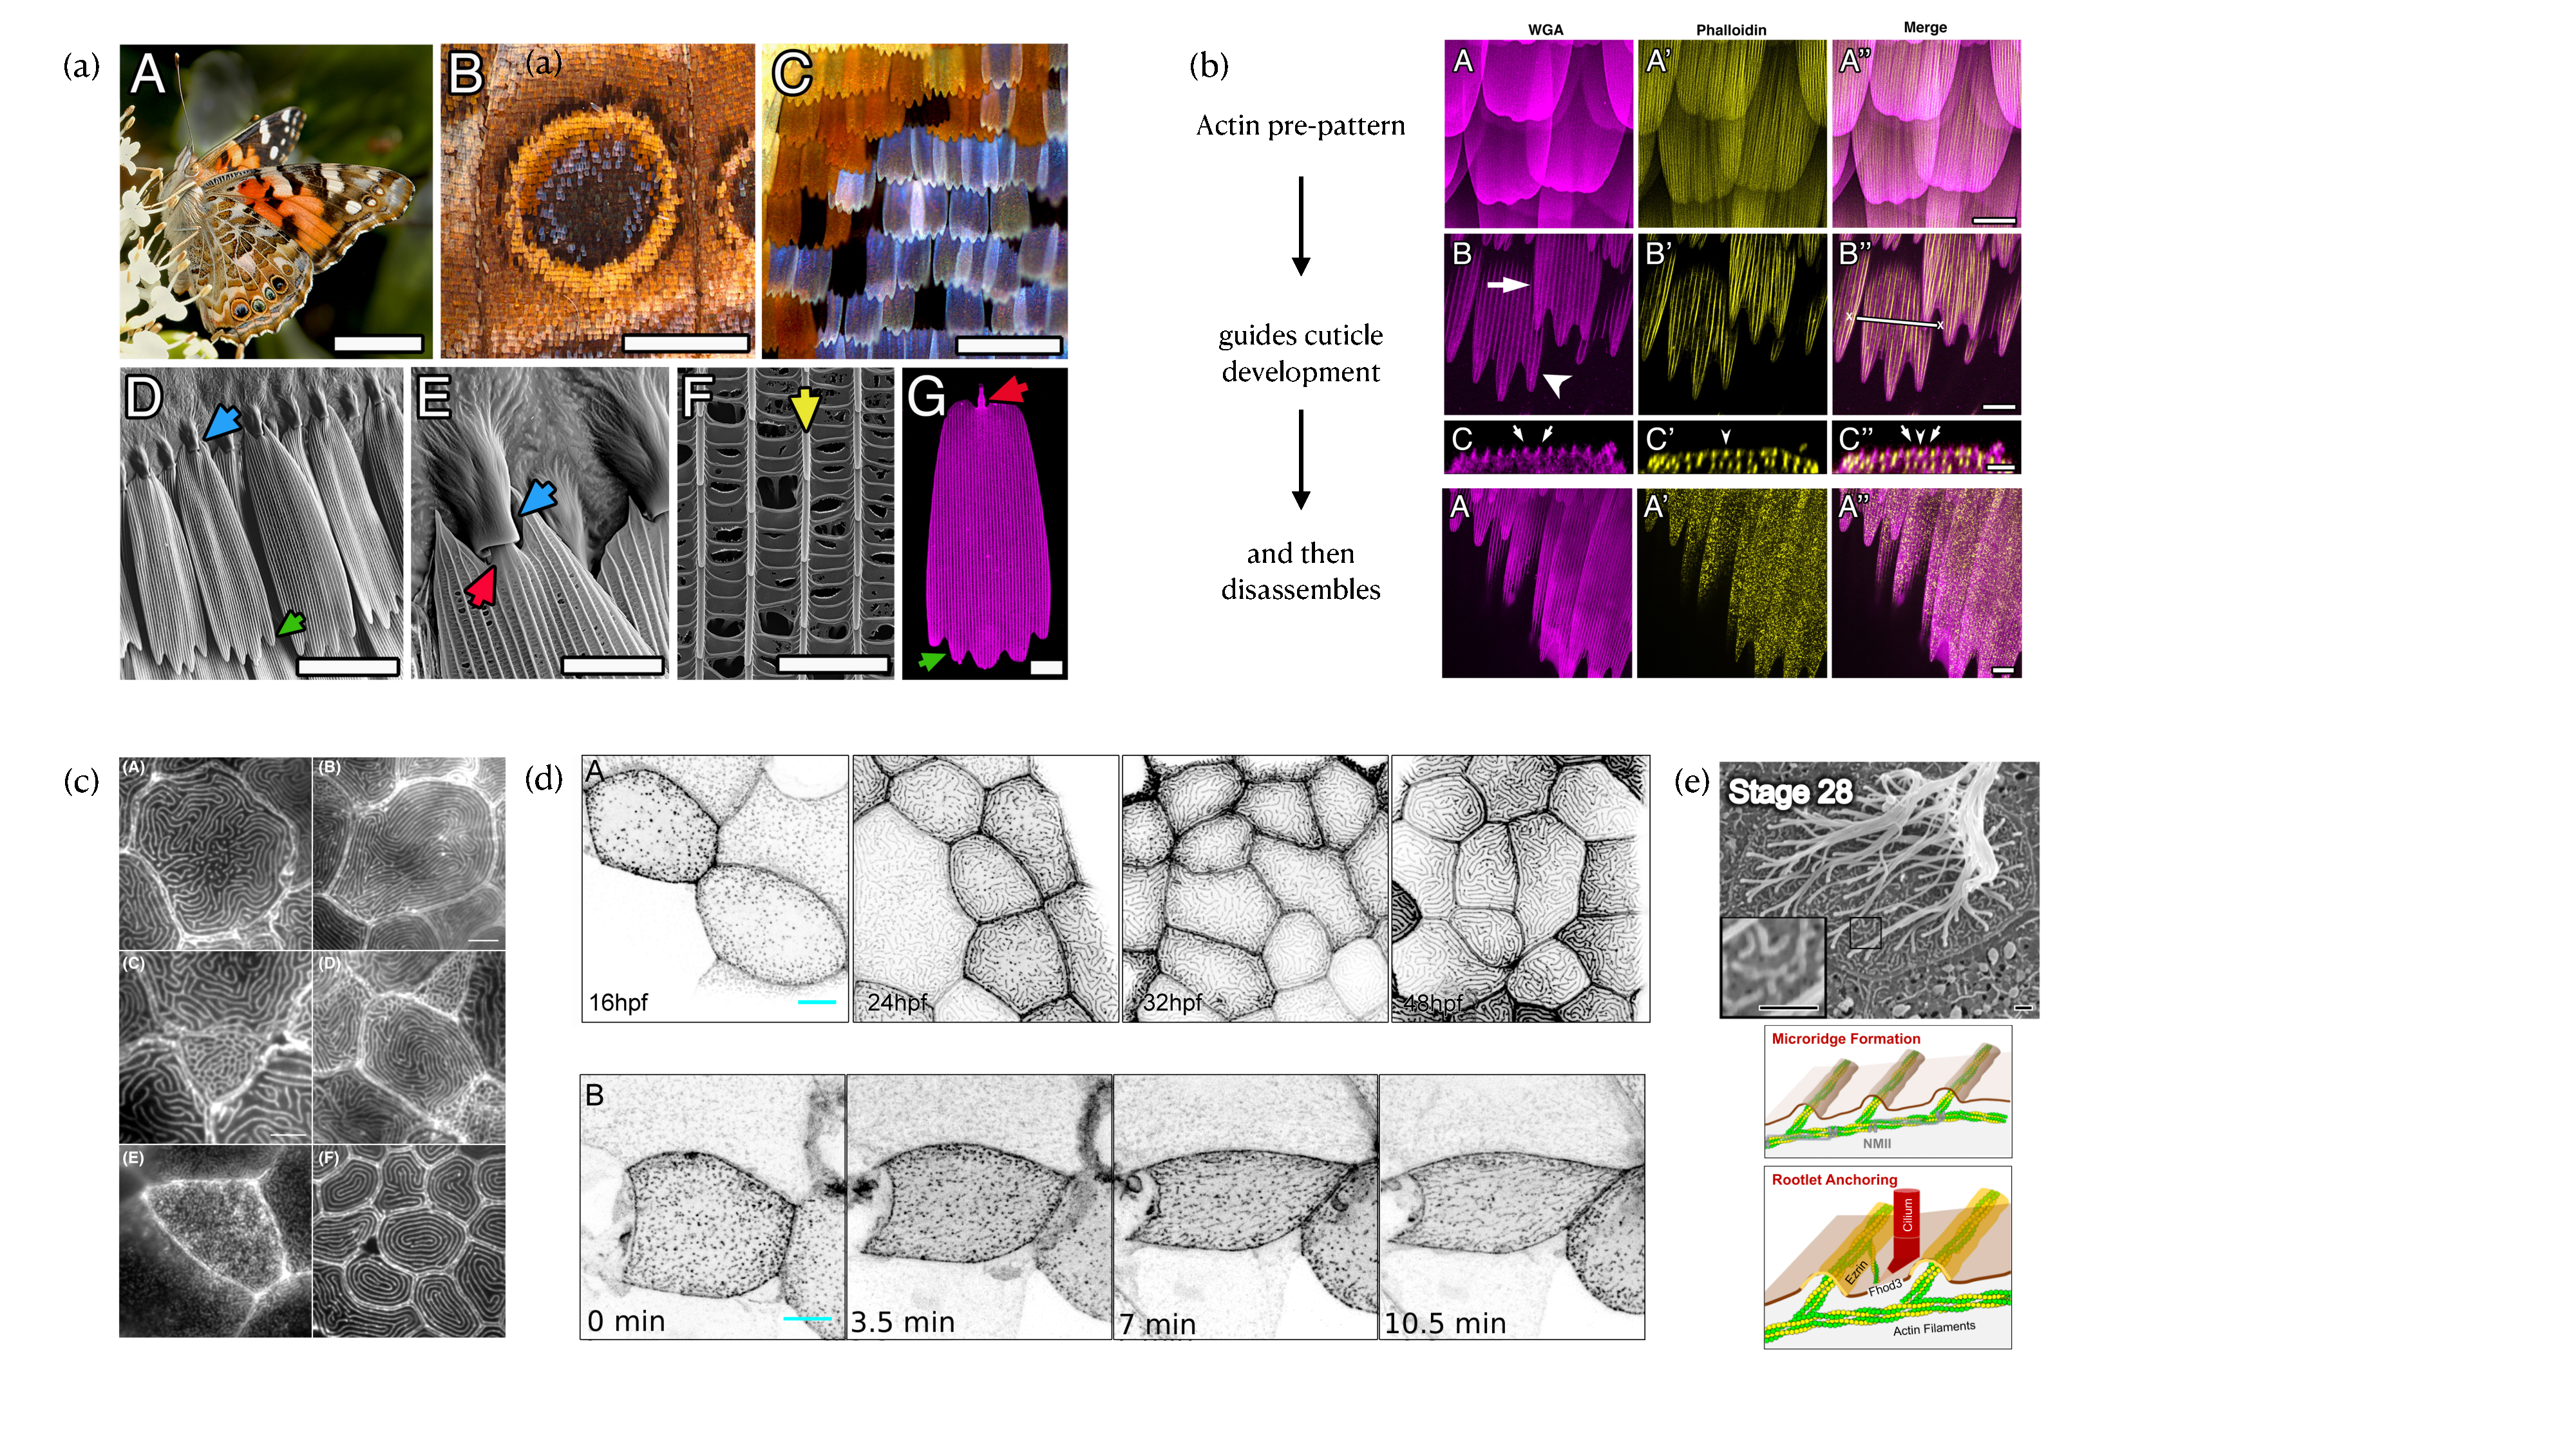
\includegraphics[width=0.99\textwidth]{actin_morphogenesis.pdf}
	\caption{\label{chap_1_fig_777} (a) Multiscale organization of the butterfly wing. Ridges in the scales are the result of the cuticle of dead cells formed from the developing wing epithelium. (b) Developmental stages starting form a pre-pattern consisting of dense parallel actin bundles, which guides the patterned deposition of the cuticle, which remains in place once the actin pre-template has disassembled \cite{DINWIDDIE2014404}.  (c) Actin microridges at the apical surfaces of scale epidermal cells in fish \cite{https://doi.org/10.1002/ar.23965} . (d) Formation of actin microridges (top) and biasing of ridge orientation by cell stretch (bottom) \cite{10.1083/jcb.201904144}. (e) Ridge-like structures template and anchor motile cilia \cite{Yasunaga:2022uh}.}
\end{figure}

\clearpage

\subsection{Microtubule networks}

Microtubules are stiff and polar cytoskeletal filaments undergoing turnover. They also form major cytoskeletal networks, which  contribute to cell shape and polarity, and support cell division and chromosome segregation through the assembly of the  spindle apparatus, Fig.~\ref{chap_1_fig_3}(a). The association of microtubules with molecular motors such as kinesins results in an extensile active gel capable of self-organization. Within cells, the physical mechanisms of the active self-organization of the spindle are becoming increasingly clear \cite{Dalton:2022wg}. Reconstituted gels of microtubules and kinesins exhibit a variety of self-organized network architectures, including patterns of asters and vortices \cite{ndlec1997, surrey2001}, Fig.~\ref{chap_1_fig_3}(b). Moreover, dense confined networks of microtubules develop persistent flows driven by the sustained nucleation, motion and annihilation of half-integer defects \cite{sanchez2012}, Fig.~\ref{chap_1_fig_3}(c). Biologically, such sustained active flows are though to drive cytoplasmic streaming \cite{serbus2005}. On a deflated vesicle, half-integer defects formed by a dense extract of microtubules and kinesins interact with the topological confinement of the closed surface to produce local geometric features of high curvature \cite{keber2014}.

\begin{figure}[hb]
	\centering
	\includegraphics[width=0.9\textwidth]{fig3.pdf}
	\caption{ \label{chap_1_fig_3} Self-organized architectures in microtubule networks. (a) Spindle apparatus during cell division (Wikipedia). (b) Patterns of asters and vortices in reconstituted microtubule-kinesin gels \cite{ndlec1997}. (c) Nucleation and motion of half-integer defects in dense microtubule-kinesin gels \cite{sanchez2012}.}
\end{figure}

\subsection{Intermediate filament networks}

Intermediate filaments (IFs) are another primary component of the cytoskeleton. These filaments are significantly more bendable than actin filaments and microtubules, longer, apolar, and undergo slow turnover \cite{broedersz2014,wagner2007,herrmann2007,godsel2008, lorenz2019}. Individual IFs can further associate into bundles through a balance of electrostatic and hydrophobic interactions \cite{haimov2020}. Although the IF molecular makeup differs widely across cell types, their hierarchical structure comprising coiled-coiled motifs that can unfold when loaded is largely preserved \cite{lorenz2019}, giving rise to the large extensibility and rate-dependent nonlinear force-elongation behavior of IFs \cite{kreplak2005, kreplak2008, qin2009}. %The force plateau upon elongation during uncoiling and the severe re-stiffening at large deformation, are the basis of the widespread view that IFs provide a ``safety belt'' against fast and large cellular deformations \cite{qin2009, golde2018, fudge2008}. 
The crosstalk between IFs and other cytoskeletal networks is receiving increasing attention \cite{huber2015}.

The self-organization of IF networks, which lack molecular motors or specific cross-linkers, into functional architectures has received relatively little attention. Recent work has shown that upon extreme stretch of epithelial monolayers, the IF network within cells undergoes a massive reorganization resulting in a structurally-optimal star-shaped architecture featuring a central node from which IF bundles radiate perpendicularly to the cell boundaries \cite{latorre2018}. Laser ablation experiments show that these taut radial IF bundles contribute to tissue resistance. Recent theoretical work suggests that this transformation is the result of self-organization controlled by network entanglement \cite{pensalfini2022}.


%\subsection{Self-organization and coexistence of actin-based architectures}
%
%Actin-based invitro or reconstituted systems self-organize diverse actin architecture, some of which coexist with each other.  For cells confined to adhesive islands of various sizes self-organize circular, radial and chiral actin bundles, see \ref{architectures}(a). Radial stress fibers and actin cluster also coexist in cells spread on adhesive substrates \cite{jalal2019} see \ref{architectures}a(right). Actin-based reconstituted systems have shown to  self-organize  a lattice of asters interconnected through actin bundles \cite{huber2015_2, weirich2017, murrell2012}, see fig \ref{architectures}(b,c,d), or form crosslinked nematic tactoid and bundles together in a suspension of actin monomers , see fig \ref{architectures}(e). Lastly, a coordinated assembly of actin bundles in hexagonal lattice drives  cellularization in a unicellular relative of animals.
%
%\begin{figure}
%	\centering
%	\includegraphics[width=0.85\textwidth]{chap_1_fig_new.pdf}
%	\caption{\label{architectures} \textbf{Self-organization and coexistence  of diverse actin-based architectures in cells and reconstituted systems}. Images adapted from (a) \citet{jalal2019} (b) \citet{huber20152} (c) \citet{adamatzky2019} (d) \citet{murrell2012} (e) \citet{weirich2017} (f)  \citet{Dudin2019}. }
%\end{figure}


\section{Theoretical models for emergent nematic cytoskeletal architectures}

The focus of this thesis is on the self-organization of nematic active gels, with an emphasis on actin networks. The self-organization of active nematic systems has been addressed using both discrete and continuous descriptions. In discrete models, \cite{bechinger2016, patelli2019, alaimo2017, ehrig2017,keber2014,khoromskaia2017,ellis2018} active nematic systems are resolved at the scale of individual active units, which are usually modeled as self-propelled Brownian particles. The emergent behavior of the system depends on an interplay of fluctuations, active forces generated by individual units, and  alignment and repulsion interactions. Discrete network simulations to specifically understand actin network show that  even obtaining a steady-state uniform network undergoing turnover and sustaining active tension is challenging \cite{freedman2018,li2017,yu2018,mak2016, hiraiwa2016, miller2018}. In general discrete models cannot access phenomena occurring at large length-scales and over long time-scales, such as those involved in the self-organization of the actin cytoskeleton at the cellular scale. Alternatively, continuum models can access the pertinent  mesoscales in time (minutes) and space (10s of microns) using fewer degrees of freedom after numerical discretization. A number of active nematic continuum models have been proposed \cite{vcopar2019,zhang2020, napoli2020,pearce2020,nestler2018,hemingway2016,metselaar2019}. The constitutive laws in these theories can be based on the underlying microscopic dynamics \cite{patelli2019,bertin2013,peshkov2012,doi:10.1126/science.aao5434,Denk:2020vm}, or on symmetry arguments within the framework of  irreversible thermodynamics \cite{simha2002,hatwalne2004,julicher2018, salbreux2022}.

\subsection{Kinematics}

At large length and time scales, the relevant dynamics of a planar nematic system can be expressed in terms of
\begin{enumerate}
	\item A change in position of material particles represented by flow field $\bm{v}(\bm{x},t)$.
	\item A change in the nematic orientational order of the system, which breaks  isotropic symmetry. At any given time, orientational order can be quantified by a coarse-grained quantity called the nematic order tensor
	\begin{align} \label{5_1}
		q_{ab}  & =  \left\langle m_a m_b - \frac{\delta_{ab}}{2}\right\rangle,
	\end{align}
	where $\bm{m} = \textup{sin}(\theta) \hat{\bm{e}}_1 + \textup{cos}(\theta) \hat{\bm{e}}_2 $ is the orientation of individual molecules and $\langle \cdot  \rangle$ represents the microscopic average of the ensemble \cite{mottram2014}. By definition, the nematic tensor is symmetric and traceless, i.e, $q_{ab}=q_{ba}$  and $q_{aa}=0$. The microscopic representation of the nematic tensor can be described in terms of a probability distribution of orientations $f(\theta)\geq 0$, which must satisfy the normalization condition  $ \int_0^{2\pi} f(\theta)d\theta=1$ and the apolar character of the network, $f(\theta) =f(\theta+\pi)$. In 2D, any symmetric and traceless tensor can be represented as
	\begin{equation}
		q_{ab} = S\left(n_a n_b -\frac{\delta_{ab}}{2}\right),
	\end{equation}
in terms of a scalar $S$ and a unit vector $\bm{n}$. Comparing this expression and Eq.~(\ref{5_1}), we identify $S= 2 \langle (\bm{m} \cdot \bm{n})^2 -1/2 \rangle$ as a measure of deviation of molecular orientation relative to the axis defined by $\bm{n}$, which can be interpreted as the net molecular orientation \cite{selinger2016}.
\end{enumerate}
\subsection{Governing equations}
The dynamics of a prototypical active nematic system follow from the coupled set of  governing equations
\begin{align}
	& \bm{\nabla} \cdot \bm{\sigma} - \bm{\nabla} p = \bm{f},   \label{12_1} \\ &
	\bm{\nabla} \cdot \bm{v} = 0 , \label{11_1}  \\ &
	\frac{d\bm{q}}{dt}  = \bm{s}(\bm{d},\bm{w}) + \frac{1}{\eta_{\rm  rot}}\bm{h},  
\end{align}
where the total stress $\bm{\sigma} = \bm{\sigma}^a + \bm{\sigma}^e + \bm{\sigma}^d$ contains an active component $\bm{\sigma}^a$, a dissipative component $\bm{\sigma}^d$ and a reversible elastic component $\bm{\sigma}^e$,  $\bm{f}$ is an external force density, and the pressure field $p$ is determined using the incompressibility constraint in Eq.~(\ref{11_1}). $d\bm{q}/dt$ is the material time derivative of $\bm{q}$, $\bm{s}$ account for changes in $\bm{q}$ due to fluid rotation and flow-induced alignment, $\eta_{\rm rot}$ is the orientational viscosity and $\bm{h}$ is the variational derivative of a free-energy potential with respect to $\bm{q}$. The free-energy potential encapsulates the equilibrium physics of the nematic system and builds on liquid-crystal theory \cite{de1993,edwards1990,beris1994}.   These governing equations are often solved with numerical algorithms such as Lattice Boltzmann methods \cite{desplat2001, denniston2004,marenduzzo2007,cates2009} or finite element methods \cite{goudiaby2021,becker2008, norton2018}.

\section{Knowledge gap}

One of the motivations to study the self-organization of active nematic gels is that the mechanisms leading to one of the most prominent architecture in the actomyosin cytoskeleton, dense nematic bundles as shown in Figs.~\ref{chap_1_fig_1} and~\ref{chap_1_fig_22}, remain poorly understood and to our knowledge no prior theory explains their mesoscale self-assembly. Previous approaches to active nematic systems have focused on incompressible liquid crystals. However, actin gels are highly porous and exhibit very large density variations controlled by advection of cortical materials, turnover, and diffusion of disassembled constituents. In turn, density controls activity and passive mechanical properties. Hence actin gels cannot be described as incompressible active fluids. Furthermore, in crowded liquid crystals, local alignment is a requirement to densely pack elongated constituents, leading to extended nematic states with defects required by topological constraints. Instead, porous actin networks can exhibit extended isotropic states without defects, and nematic order is presumably induced by flows and by active mechanisms. Finally, little attention has been paid to the formulation of active nematics on deformable surfaces, despite the fact shape and nematic architecture are strongly linked  both in cells and in reconstituted vesicle systems  \cite{anne2016, Dong,mandato2001,weirich2019,keber2014}. Recent exceptions are the theoretical framework by \citet{salbreux2022} and the computational study by \citet{https://doi.org/10.48550/arxiv.2205.06805}. In addition to model formulation, the field lacks a general computational framework capable of solving the multi-field governing equations in their full nonlinearity, including the coupling between in-plane density-dependent active nemato-hydrodynamics and shape. Finally, we lack a unified understanding of actin network polymorphism, and more specifically of the physical mechanisms that enable a single active material to adopt very different network architectures with distinct cellular functions. 


\section{Goals and objectives}

This thesis has two main goals. The first goal is to understand the physical mechanisms that control the active self-organization of the actin cytoskeleton into diverse nematic architectures, focusing on 2D gels representative of a flat actomyosin cortex.  To achieve this goal, we establish the following objectives:
\begin{enumerate}
	\item Develop a thermodynamically consistent mathematical model of an active nematic gel and pertinent to the actin cytoskeleton, in particular accounting for the appropriate mechanisms coupling density, hydrodynamics and nematodynamics.
	\item Develop a numerical framework to approximate the solution of the proposed mathematical model in biologically relevant situations.
	\item Perform a linear stability analysis of the model to map the parameter regions where destabilization of a homogeneous steady state leads to pattern formation.
	\item Perform simulations to study the fully nonlinear behavior of the self-organized patterns in different parametric regimes of the model.
	\item Identify the key parameters that control actin gel polymorphism and dynamics.
	\item Validate key assumptions of the active nematic gel theory using discrete network simulations of the cytoskeleton.
\end{enumerate}
The second goal of the thesis is to explore the spontaneous shape changes in curved active nematic gels resulting from the self-organization of different network architectures. To reach this goal, we establish the following objectives:
\begin{enumerate}
	\item Extend the proposed 2D active nematic gel theory to arbitrarily curved and deformable surfaces in a covariant and thermodynamically consistent manner.
	\item Develop numerical algorithms to solve the active nematic gel theory under the assumption of axisymmetry to efficiently explore relevant morpho-nemato-hydrodynamical processes such as cell division.
	\item Develop general numerical algorithms in 3D to active nematic gel theory on deformable surfaces and apply it to relevant morpho-nemato-hydrodynamical processes.
\end{enumerate}

\section{Thesis outline}

The Thesis is structured as follows. In the first part, we address the  first goal of the thesis in the following sequence
\begin{enumerate}
\item In Chapter~\ref{chap_2}, we first introduce Onsager's variational formalism as an elegant and useful framework to model the dissipative and active dynamics of biological systems. Based on this formalism, we then develop a general theory for density-dependent active nematic gels.
\item In Chapter~\ref{chap_3}, we present a finite element computational framework to numerically solve the governing equations. We then apply the numerical model to explore wound healing mechanisms in actin gels and self-organized flows and patterns of defects in confined colonies of elongated cells.
\item In Chapter~\ref{chap_4}, we test the idea of physical self-organization of actin nematic architectures. To understand the onset of pattern formation, we perform linear stability analysis of the dynamical equations, leading to explicit formulae for the critical activity required to produce out-of-equilibrium patterns consisting of dense nematic structures coexisting with a low-density isotropic network. We then examine the fully nonlinear regime using simulations and identify physical principles controlling the geometry and dynamics of emergent patterns.
Furthermore,  we seek to validate key assumptions in our active nematic  gel theory required for self-organization of dense nematic bundles. For this, we drive out-of-equilibrium an agent-based microscopic model of the actomyosin network to characterize active tension anisotropy and nematic activity.
\end{enumerate}

In the second part, we address the second goal of the thesis in the following sequence
\begin{enumerate}
	\item In Chapter~\ref{chap_6}, we motivate through experimental observations the investigation of shape changes in active nematic surfaces.
\item In Chapter~\ref{chap_7}, we present a  thermodynamically consistent theoretical framework based on Onsager's variational formalism for density-dependent active nematic gels on deformable surfaces.
\item In Chapter~\ref{chap_8}, we present a computational framework to solve the axisymmetric governing equations, which we use to study the self-organized shape changes in actin cortices  during cell division and polarization.
\item In Chapter~\ref{chap_9},  we present a theoretical and computational 3D framework for the coupled nematic and shape dynamics in an inextensible active liquid crystalline surface, and use it to examine the interaction between shape and defects.
\end{enumerate}
Finally, in Chapter~\ref{chap_10}, we summarize our contributions and outline future avenues of research.


\renewcommand{\thesection}{2.\arabic{section}}
\part{Active self-organization of nematic architectures on a flat surface}
\chapter{A variational framework for 2D active nematic gels} \label{chap_2}
\section{Introduction}

Active nematic systems are far-from-equilibrium materials characterized by broken rotational symmetry due to the local orientational order of the constituents. This asymmetry allows the energy-consuming constituents to apply anisotropic forces at a local scale leading to system-scale directional deformations. Such systems are ubiquitous in living matter, and include the actin cytoskeleton \cite{chugh2018}, microtubule and kinesin gels \cite{ndlec1997}, colonies of muscle cells \cite{duclos2014,guillamat2020}, swarms of sperm cells \cite{creppy2015},  dense bacterial suspensions \cite{qi2022, gachelin2014} and epithelial cell cultures \cite{maroudas2021,blanch2018,saw2017}. Often, these systems organize as 2D or quasi-2D material layers.
Understanding the underlying mechanism responsible for the emergence of macro- and meso-scale organizations due to micro-scale anisotropic activity is still an open challenge. Addressing this question can improve our understanding of the dynamics of living matter and potentially help us design biomimetic engineered materials \cite{fratzl2007}.

Mathematical models are widely used to explore complex systems by mapping the system of interest to mathematical equations, which can be examined analytically or numerically. Mathematical modeling of active matter in general, or the actin cytoskeleton in particular, is particularly challenging as one needs to distinguish passive dissipative and thermodynamic mechanisms from activity in a consistent manner irrespective of nonlinearity \cite{Prost:2015aa}. Formulating such models  requires a conceptual framework to guide  rational choices based on the underlying physics of the system of interest. In this context, Onsager's variational formalism provides a systematic workflow to derive fully nonlinear, multiphysics, and thermodynamically consistent mathematical models for active biological systems where inertial forces do not play a role. This framework is an extension of Rayleigh’s principle of the least energy dissipation principle \cite{Rayleigh1873} for general irreversible processes, and has been used in a number of different contexts under different names, including soft and biological matter \cite{doi2011,doi2012,arroyo2018,torres2019}.  Onsager's reciprocal relations  \cite{Onsager1931} follow naturally from this modeling formalism.


\section{Abstract statement of the Onsager's variational formalism}

We describe a dissipative system with the following key ingredients that will later serve as building blocks for the Onsager's variational formalism:
\begin{enumerate}
	\item Coarse-grained state variables $\bm{X} = \{X_1, X_2, ....X_n \}$ that identify the non-equilibrium state of the system.
	\item Free-energy potential $\mathcal{F}$ that depends on the state variables $\bm{X}$ and measures the energy available in the system to do work.
	\item Process variables $\bm{V} = \{V_1, V_2, ....V_n \}$ that describe the time evolution of the state of the system.
	\item The process operator $\mathbb{P}$, which relates the rate of change of the state variables and the process variables, i.e., $ \partial_t X_i = \mathbb{P}(\bm{X})V_i $. The process operator $\mathbb{P}$ can be trivial, i.e, $	\partial_t X_i=V_i $, or non-trivial when expressed as conservation equations, possibly involving Lie derivatives when state variables are tensor quantities.
	\item Dissipation potential $\mathcal{D}$ encoding dissipative mechanisms.
	\item Power functional $\mathcal{P}$ that encodes the external power input, e.g.~due to chemo-mechanical transduction or through boundary conditions. 
	\item A functional $\mathcal{Q}$ encoding the power done on the system by the physical constraints.
\end{enumerate}

Defining the functional form of functionals $\mathcal{F}$ and $\mathcal{D}$ determines the constitutive relations associated to passive components of the system, whereas all activity is encoded in $\mathcal{P}$.

The rate of change of the free energy potential is computed using the chain rule as
\begin{align}
	\dot{\mathcal{F}}(\bm{X};\bm{V}) =    \frac{d}{dt}\left(\mathcal{F}(\bm{X})\right)   =  \sum_{i=1}^n \partial_{X_i} \mathcal{F} \partial_t X_i 	=  \sum_{i=1}^n \partial_{X_i} \mathcal{F}\, \mathbb{P}(\bm{X})V_i. 
\end{align}
In applications, the calculations of $\dot{\mathcal{F}}(\bm{X};\bm{V})$ may imply using  Reynold's transport theorem. The dissipation potential $\mathcal{D}\left(\bm{X};\bm{V}\right)$ can be non-linear in $\bm{X}$, but is often a quadratic function of process variables $\bm{V}$. As per the thermodynamic requirements, $\mathcal{D}$ has to be non-negative, i.e, $\mathcal{D}(\bm{X},\bm{V}) \geq 0$, should be zero when the system does not evolve, i.e, $\mathcal{D}(\bm{X},0)=0$. A prototypical dissipation potential  $\mathcal{D}$ can be written as
\begin{equation}
	\mathcal{D}\left(\bm{X};\bm{V}\right) = \sum_{i=1}^{n}\sum_{j=1}^{n}V_i L_{ij}(\bm{X}) V_j,
\end{equation}
where  $L_{ij}=L_{ji}$ and $\bm{L}$ is a positive definite matrix of material coefficients according to Onsager's reciprocity relationship \cite{Onsager1931}, ensuring positivity of dissipation. The power potential $\mathcal{P}(\bm{X};\bm{V})$, in its simplest form, can be written as 
\begin{equation}
	\mathcal{P}(\bm{X};\bm{V}) = \sum_{i=1}^{n} \mathpzc{P}_{i}(\bm{X}) V_i.
\end{equation}
The constraint potential $\mathcal{Q}(\bm{X};\bm{V},\bm{\Lambda})$ is formulated as  
\begin{equation}
	\mathcal{Q}(\bm{X};\bm{V},\bm{\Lambda}) = \sum_{i=1}^{m}   \sum_{k=1}^{n} \Lambda_i C_{ik}(\bm{X})V_k ,
\end{equation}
where $C_{ij}$ is a matrix encoding constraints with $m<n$ and $\bm{\Lambda} = \{\Lambda_1, \Lambda_2, ... , \Lambda_m \}$ is a vector of Lagrange multipliers that enforces  $\bm{C}(\bm{X})\cdot \bm{V} = \bm{0}$.  By adding the aforementioned potential functions, we  form the Rayleighian as
\begin{equation}
	\mathcal{R}(\bm{X};\bm{V}) =  \dot{\mathcal{F}}(\bm{X};\bm{V}) + \mathcal{P}(\bm{X};\bm{V}) + \mathcal{D}(\bm{X};\bm{V}) .
\end{equation}
This functional captures the competition between free-energy relaxation, power input and dissipation.
Onsager’s variational principle then states that the system evolves such that
\begin{equation}
	\bm{V}  = \underset{\bm{W}}{\textup{argmin}} \, \, \mathcal{R}(\bm{X}; \bm{W}),
\end{equation}
subjected to constraints on $\bm{W}$ as 
\begin{equation}
	\sum_{j=1}^{n}	C_{ij}(\bm{X}) W_j =0.
\end{equation}
The constrained dynamics can be equivalently characterized as saddle points of the Lagrangian 
\begin{equation}
	\mathcal{L}(\bm{X};\bm{V},\bm{\Lambda}) = 	\sum_{i=1}^n \left[\partial_{X_i} \mathcal{F}\,\mathbb{P}(\bm{X}) + \mathpzc{P}_i(\bm{X}) +  \sum_{j=1}^n \left(  L_{ij}(\bm{X})V_j    -   \Lambda_j  C_{ji}(\bm{X}) \right) \right]V_i .
\end{equation}
The stationary condition $\delta_{\Lambda_i}\mathcal{L}=0$ leads to the following set of $n$ constraints
\begin{equation}
	C_{ij}(\bm{X}) V_j=0,
\end{equation}
The stationary condition $\delta_{V_i}\mathcal{L}=0$ leads to  following set of $n$ governing equations that drive the evolution of the active system of interest
\begin{equation}
\partial_{X_i} \mathcal{F}\,\mathbb{P}(\bm{X}) + \mathpzc{P}_i(\bm{X}) +  \sum_{j=1}^n \left( 2L_{ij}(\bm{X})V_j    -   \Lambda_j  C_{ji}(\bm{X}) \right)  = 0.
\end{equation}
  Towards studying active nematic systems with possibly time-dependent density in their full nonlinearity, in the following sections we develop a systematic and simple modeling framework for density-dependent active nemato-hydrodynamics using  Onsager's formalism. This theory is thermodynamically consistent ab initio, is complementary to more standard approaches based on irreversible thermodynamics for active gels \cite{Prost:2015aa,julicher2018}.


	
\section{Description of an active nematic gel} \label{sec_1}

We consider a planar thin sheet of a nematic material. We describe this system with a density field $\rho(\bm{x},t)$ and with a nematic tensor field 
\begin{equation} 
	\label{eq:nematic_tensor}
	\bm{q}(\bm{x},t) =S(\bm{x},t) \left[\bm{n}(\bm{x},t) \otimes \bm{n}(\bm{x},t) - \frac{1}{2}\bm{I}\right] ,
\end{equation}
where $\bm{I}$ is the 2D identity tensor, $\bm{n}$ is a unit vector representing the average nematic alignment and $S=\sqrt{2 q_{ab}q_{ab}}$ is the nematic order parameter, which measures the strength of the nematic alignment about $\bm{n}$. In general, $S \in [0,1]$, where $\textit{S}=0$ and $\textit{S}=1$ represent limit cases where nematic particles are isotropically distributed and perfectly aligned about $\bm{n}$, respectively. We note that $\bm{q}$ is symmetric and traceless, i.e., $\bm{q}=\bm{q}^T$ and $\text{tr}\bm{q}=0$. At any given time, the state of the system is represented by the nematic order tensor $\bm{q}$ and the density field $\rho$.

To describe how the system changes its state, we consider the macroscopic velocity field $\bm{v}$. We decompose its gradient  into a symmetric and an antisymmetric parts
\begin{align} \label{gradv}
	\nabla \bm{v}  = \bm{d} + \bm{w},
\end{align}
where 
\begin{align}
	\label{eq:rate-of-deformation}\bm{d} &= \frac{1}{2}\left[\nabla \bm{v} +\left( \nabla\bm{v}\right)^T\right],\\ 
	\label{eq:spin}\bm{w} &= \frac{1}{2}\left[\nabla \bm{v} -\left( \nabla\bm{v}\right)^T\right].
\end{align}
The tensor $\bm{d}$ characterizes the rate of deformation of a differential of volume of the material and it is usually referred to as the \textit{rate-of-deformation tensor}. This tensor plays an important role in different aspects of the theory. For instance, $\text{tr}\bm{d}=\nabla \cdot \bm{v}$ characterizes the rate of accumulation or dilution of density and its deviatoric part of $\bm{d}^{\rm dev} = \bm{d}  - \frac{1}{2}(\text{tr}\bm{d})\bm{I}$ identifies the shear rate leading to energy dissipation. The tensor $\bm{w}$ describes the local rate of rotation generated by the flow, possibly leading to rotation of the nematic alignment, and it is referred to as the \textit{spin tensor}; note that in 2D it can be represented with a single scalar $\bm{w}=w\bm{\epsilon}$, where $\bm{\epsilon}$ is the Levi-Civita tensor. The gradient of the spin is given by 
\begin{equation} 
	\bm{\zeta} = \nabla w \, .
\end{equation} 
The rate of change of $\rho$ is characterized by a conservation law of the form
\begin{equation}
	\label{eq:balance_mass}
	\dot{\rho} + \rho {\rm tr}\bm{d} = r ,
\end{equation}
where $\dot{\rho}(\bm{x},t) = \partial_t \rho(\bm{x},t) + \bm{v}(\bm{x},t)\cdot\nabla\rho(\bm{x},t)$ is the material time-derivative of $\rho$. The second term characterizes the dilution (or compaction) of $\rho$ driven by the rate of change of the differential of area characterized by the trace of $\bm{d}$, and $r$ is the rate of change of density not explained by the flow $\bm{v}$, typically resulting from a chemical reaction or a diffusive flux.  We characterize the rate of change of $\bm{q}$ with the Jaumann derivative \cite{de1993}.
\begin{equation}
	\label{eq:Jaumann}
	\widehat{\bm{q}}= \dot{\bm{q}}  + \bm{q}  \cdot \bm{w} -  \bm{w}  \cdot \bm{q},
\end{equation}
or in components as
\begin{equation} \label{jaumann_detivative_def}
	\widehat{q}_{ab} = \dot{q}_{ab}  + q_{ac} w_{cb} - w_{ac} q_{cb}.
\end{equation}
where $ \dot{q}_{ab} = \partial_t q_{ab} + v_c \nabla_c q_{ab}$ is the total time derivative of the nematic order tensor.  We note that $\widehat{\bm{q}}$ measures the rate of change of $\bm{q}$ viewed by an observer that flows and rotates with $\bm{v}$; thus, $\widehat{\bm{q}}$ is zero if $\bm{q}$ is advected and rotated by the flow without any further rearrangements of the nematic field. 

\section{Governing equations from Onsager's formalism} \label{sec:Onsager}


We derive next the governing equations of an active nematic gel at low Reynolds numbers. Let $A \subset \mathbb{R}^2$ be an open set and its boundary $\partial A$ be sufficiently smooth. The unit outward normal to $\partial A$ is denoted by $\bm{N}$.  We denote by  $\bm{t}$, $\bm{\Gamma}$ and $\bm{L}$ the boundary generalized forces power-conjugate to $\bm{v}$,  $\bm{w}$ and  $\widehat{\bm{q}}$, respectively, which we call traction, moment and microscopic moment and act on the boundaries $\partial_{N_{\bm{t}}} A $, $\partial_{N_{\bm{\Gamma}}} A $ and $\partial_{N_{\bm{L}}} A $, see Fig.~\ref{fig0}.

\begin{figure}[H]
	\centering
	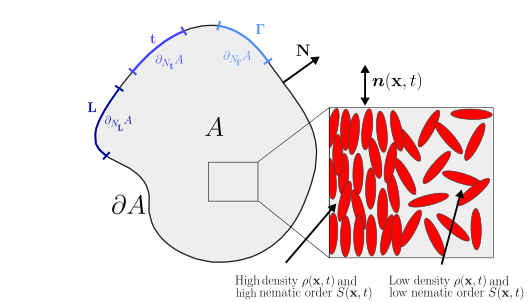
\includegraphics[width=0.75\textwidth]{chap_2_fig_1.pdf}
	\caption{\label{fig0}  \textbf{Schematic of a compressible active nematic gel}. The system occupies  a region $A$ with boundary $\partial A$ and unit outer boundary normal $\bm{N}$. Traction $\bm{t}$, moment $\bm{\Gamma}$ and microscopic moment $\bm{L}$ act on the  boundaries $\partial_{N_{\bm{t}}} A $, $\partial_{N_{\bm{\Gamma}}} A $ and $\partial_{N_{\bm{L}}} A $, respectively. The active nematic system exhibits spatiotemporal variations in density $\rho(\bm{x},t)$ and the nematic order tensor $\bm{q}(\bm{x},t)$, parametrized by the nematic order parameter $S(\bm{x},t)$ and the average molecular orientation $\bm{n}(\bm{x},t)$, Eq.~(\ref{eq:nematic_tensor}), represented with a double-headed arrow.
	}
\end{figure}
%To derive the strong form, we follow a non-linear Onsager's variational formalism. The formalism, an extension of Rayleigh’s principle of the least energy dissipation principle \cite{Rayleigh1873}, is based on the minimization of a Rayleighian functional $R = \dot{\mathcal{F}} + \mathcal{D} + \mathcal{P}$, where $\mathcal{F}$, $\mathcal{D}$ and $\mathcal{P}$ are the free energy, dissipation and power potential, repectively, possibly subject to constraints  \cite{doi2012, arroyo2018}. 

We postulate generic forms for the free-energy functional $\mathcal{F}$, dissipation functional $\mathcal{D}$ and power functional $\mathcal{P}$ as
\begin{align}
	\mathcal{F}\left[\rho,\bm{q}\right] &= \underset{A}{\int} f(\bm{q},\nabla\bm{q}) \rho dA, \label{eq:free_energy}\\
	\mathcal{D}\left[\bm{v},\widehat{\bm{q}}; \rho,\bm{q}\right] &= \underset{A}{\int} d(\bm{v},\bm{d},\bm{w},\bm{\zeta},\widehat{\bm{q}}) \rho dA,\\
	\mathcal{P}\left[\bm{v},\widehat{\bm{q}}; \rho,\bm{q}\right] &= \underset{A}{\int} p(\bm{v},\bm{d},\bm{w},\bm{\zeta},\widehat{\bm{q}}) \rho dA - \int_{\partial_{N_{\bm{t}}} A} \bm{t} \cdot \bm{v} dl -  \int_{\partial_{N_{\bm{\Gamma}}} A} \bm{\Gamma}:\bm{w} dl -  \int_{\partial_{N_{\bm{L}}} A} \bm{L}:\widehat{\bm{q}} dl,
\end{align}
where the integrands in the first three integrals are the free-energy, dissipation, and power input densities. Towards applying Onsager's variational formalism, we need to compute the rate of change of Eq.~(\ref{eq:free_energy}), for which we apply the Reynold's transport theorem 
\begin{equation}
	\begin{aligned} \label{eq:change_of_free_energy}
		\dot{\mathcal{F}} &= \underset{A}{\int} \left[\partial_tf  \rho + f \partial_t{\rho} \right] dA + \int_{\partial A} f\rho \bm{v} \cdot\bm{N} ~dl\\
		&= \underset{A}{\int} \left[\partial_tf  \rho + f \partial_t{\rho}  + \nabla\cdot\left(f\rho \bm{v}\right) \right] dA\\
		&=\underset{A}{\int} \left[\dot{f}  \rho + f \dot{\rho}  + f\rho {\rm tr}\bm{d} \right] dA.
	\end{aligned}
\end{equation}
The rate of change of $f$ can be computed as
\begin{equation}
	\begin{aligned}
		\label{eq:dotfU}  
		\dot{f} &=  \frac{\partial f}{\partial q_{ab}} \dot{q}_{ab}+ \frac{\partial f}{\partial \nabla_c q_{ab}} \dot{\nabla q}_{abc}\\
		&= \frac{\partial f}{\partial q_{ab}}\left(\widehat{q}_{ab}- q_{ad} w_{db}- q_{db} w_{da}\right) \\
		&~~~+  \frac{\partial f}{\partial \nabla_c q_{ab}}\left(\widehat{\nabla q}_{abc}-\nabla_cq_{ad} w_{db}- \nabla_cq_{db} w_{da}- \nabla_d q_{ab} w_{dc} \right), 
	\end{aligned}
\end{equation}
where $\dot{\nabla q}_{abc} = \left(\partial_t \nabla_c q_{ab} + \nabla_d \nabla_c q_{ab} v_d\right)$ and $\widehat{\nabla q}_{abc} = \dot{\nabla q}_{abc} +\nabla_cq_{ad} w_{db}+ \nabla_cq_{db} w_{da}+ \nabla_d q_{ab} w_{dc}$. We now note that $f$ must be invariant with respect to rigid body rotations, i.e.~when $d_{ab}=0$, $\widehat{q}_{ab}=0$, $\dot{f}=0$ for any $w_{ab}$. This condition can be written as
\begin{equation}
	\begin{aligned}
		0 &= \bigg[ \frac{\partial f}{\partial q_{ad}} q_{bd}  - \frac{\partial f}{\partial q_{bd}} q_{ad}  + \frac{\partial f}{\partial \nabla_c q_{ad}} \nabla_cq_{bd}-\frac{\partial f}{\partial \nabla_c q_{bd}}  \nabla_c q_{ad} \\
		&~~~+ \frac{1}{2} \left(\frac{\partial f}{\partial \nabla_a q_{cd}} \nabla_b q_{cd}-\frac{\partial f}{\partial \nabla_b q_{cd}} \nabla_a q_{cd}\right) \bigg] w_{ab},
	\end{aligned}
\end{equation}
which being valid for all spins, leads to the constraint 
\begin{equation}
	\begin{aligned}
		0 &=  \frac{\partial f}{\partial q_{ad}} q_{bd}  - \frac{\partial f}{\partial q_{bd}} q_{ad}  + \frac{\partial f}{\partial \nabla_c q_{ad}} \nabla_cq_{bd}-\frac{\partial f}{\partial \nabla_c q_{bd}}  \nabla_c q_{ad} \\
		&~~~+ \frac{1}{2} \left(\frac{\partial f}{\partial \nabla_a q_{cd}} \nabla_b q_{cd}-\frac{\partial f}{\partial \nabla_b q_{cd}} \nabla_a q_{cd}\right). 
	\end{aligned}
\end{equation}
This constraint is usually referred to as Gibbs-Duhem relation \cite{julicher2018}. Using this relation, the symmetry of $\bm{q}$ and the fact that the tensor product of a symmetric  and an antisymmetric tensor is zero, Eq.~(\ref{eq:dotfU}) reduces to
\begin{equation}
	\label{eq:dotfU2}  
	\dot{f}= \frac{\partial f}{\partial q_{ab}} \widehat{q}_{ab} +  \frac{\partial f}{\partial \nabla_c q_{ab}}\widehat{\nabla q}_{abc}.
\end{equation}
Using Eq.~(\ref{gradv}), the definition of the Levi-Civita tensor and the product rule,  the Jaumann derivative of $\nabla \bm{q}$ can be written in terms of the Jaumann derivative of $\bm{q}$ as
\begin{equation}
	\begin{aligned}
		\widehat{\nabla q}_{abc} &= \partial_t \nabla_c q_{ab} + v_d \nabla_d \nabla_c q_{ab} + \nabla_c q_{ad} w_{db} + \nabla_c q_{db} w_{da} + \nabla_d q_{ab} w_{dc}\\
		&= \nabla_c \widehat{q}_{ab} - \nabla_c v_d \nabla_d q_{ab} - q_{ad} \nabla_c w_{db} - q_{db} \nabla_c w_{da} + \nabla_d q_{ab} w_{dc}\\
		&= \nabla_c \widehat{q}_{ab} - d_{dc} \nabla_d q_{ab} - q_{ad} \nabla_c w_{db} - q_{db} \nabla_c w_{da} \\
		&= \nabla_c \widehat{q}_{ab} - d_{dc} \nabla_d q_{ab} + \left(\epsilon_{ad} q_{db} - q_{ad}  \epsilon_{db} \right) \zeta_c.
	\end{aligned}
\end{equation}
We thus can write
\begin{equation}
	\dot{f} = \frac{\partial f}{\partial q_{ab}}\widehat{q}_{ab} + \frac{\partial f}{\partial \nabla_c q_{ab}}\left[ \nabla_c \widehat{q}_{ab} - d_{dc} \nabla_d q_{ab} + \left(\epsilon_{ad} q_{db} - q_{ad}  \epsilon_{db} \right) \zeta_c\right].
\end{equation}
Plugging this expression in Eq.~(\ref{eq:change_of_free_energy}), we obtain
\begin{equation}
	\begin{aligned}
		\label{eq:dotF}
		\dot{\mathcal{F}}[\dot{\rho},\widehat{\bm{q}},\bm{d},\bm{\zeta};\rho,\bm{q}] = \int_{A} &\left\{ f \left(\frac{\dot{\rho}}{\rho}+{\rm tr} \bm{d}\right)  +\frac{\partial  f}{\partial \bm{q}} : \widehat{\bm{q}}\right.\\ 
		&\left.+ \frac{\partial  f}{\partial \nabla \bm{q}} \cdddot \, \left[\nabla \widehat{\bm{q}} - \left(\nabla \bm{q}\right)^T \cdot\bm{d} +\left(\bm{\epsilon} \cdot \bm{q} - \bm{q} \cdot \bm{\epsilon}\right)\otimes \bm{\zeta} \right]\right\} \rho dA.
	\end{aligned}
\end{equation}
For clarity of our derivation, we consider the fields $\dot{\rho}$, $\bm{d}$, $\bm{w}$ and $\bm{\zeta}$ as independent variables, and enforce the kinematic and conservation relations relating them through Lagrange multipliers. Thus, the Rayleighian has the form
\begin{align}
	\label{eq:Rayleighian}
	\mathcal{R}\left[\dot{\rho},\bm{v},\bm{d},\bm{w},\bm{\zeta},\widehat{\bm{q}};\rho,\bm{q}\right] = & \dot{\mathcal{F}}[\dot{\rho},\bm{d},\bm{\zeta},\widehat{\bm{q}};\bm{q},\rho] + 
	\mathcal{D}\left[\bm{v},\bm{d},\bm{w},\bm{\zeta},\widehat{\bm{q}}; \bm{q},\rho\right] +  \\ & \mathcal{P}\left[\bm{v},\bm{d},\bm{w},\bm{\zeta},\widehat{\bm{q}}; \bm{q},\rho\right], \nonumber
\end{align}
and the governing equations can then be obtained by minimizing it with respect to the process variables $\dot{\rho}, \bm{v},\bm{d},\bm{w},\bm{\zeta}$ and $\widehat{\bm{q}}$ and enforce kinematic and mass conservation constraints with the constraint functional
\begin{equation}
	\label{eq:constraints}
	\begin{aligned}
		\mathcal{Q}[\varrho, \bm{\sigma}^{\rm s}, \bm{\sigma}^{\rm a},\bm{m}, \dot{\rho},\bm{v},\bm{d},\bm{w},\bm{\zeta},\widehat{\bm{q}};\rho,\bm{q}] =
		& \underset{A}{\int} \varrho  \left[\dot{\rho} + \rho{\rm tr}\bm{d}- r\right] dA  + \\
		& \underset{A}{\int} \bm{\sigma}^{\rm s} :\left[\bm{d} - \frac{1}{2}\left(\nabla \bm{v} + \left(\nabla\bm{v}\right)^T\right)\right] dA + \\
		& \underset{A}{\int} \bm{\sigma}^{\rm a} :\left[\bm{w} - \frac{1}{2}\left(\nabla \bm{v} - \left(\nabla\bm{v}\right)^T\right)\right] dA + \\
		& \underset{A}{\int} \bm{m} \cdot \left[\bm{\zeta} - \nabla w\right] dA,
	\end{aligned}
\end{equation}
where $\varrho $ is the Lagrange multiplier imposing balance of mass; $\bm{\sigma}^{\rm s}$, a symmetric tensor, and $\bm{\sigma}^{\rm a}$, an antisymmetric tensor, are the Lagrange multipliers imposing the definitions of the rate-of-deformation and spin tensors; and $\bm{m}$, a vector, is the Lagrange multiplier imposing the definition of the gradient of the spin.  We thus form the  potential as 
\begin{equation}
	\label{eq:Lagrangian} 
	\begin{aligned}
		\mathcal{L}[\varrho, \bm{\sigma}^{\rm s}, \bm{\sigma}^{\rm a},\bm{m},\dot{\rho},\bm{v},\bm{d},\bm{w},\bm{\zeta},\widehat{\bm{q}};\rho,\bm{q}] =~& \mathcal{R}[\dot{\rho},\bm{v},\bm{d},\bm{w},\bm{\zeta},\widehat{\bm{q}};\rho,\bm{q}] -  \\
		&\mathcal{Q}[\varrho, \bm{\sigma}^{\rm s}, \bm{\sigma}^{\rm a},\bm{m}, \dot{\rho},\bm{v},\bm{d},\bm{w},\bm{\zeta},\widehat{\bm{q}};\rho,\bm{q}],
	\end{aligned}
\end{equation}
whose minimization with respect to the process variables leads to the governing equations. Arbitrary variations of $\widehat{\bm{q}}$ lead to
\begin{equation}
	\label{eq:var_q}
	\begin{aligned}
		0&=\underset{A}{\int} \left[ \left(\frac{\partial  f}{\partial \bm{q}} + \frac{\partial d}{\partial \widehat{\bm{q}}}+ \frac{\partial p}{\partial \widehat{\bm{q}}} \right) : \delta \widehat{\bm{q}} + \frac{\partial f}{\partial \nabla \bm{q}} \cdddot\, \nabla \delta \widehat{\bm{q}} \right] \rho dA - \int_{\partial_{N_{\bm{L}}}A} \bm{L}:\delta\widehat{\bm{q}} dl \\
		&=\underset{A}{\int} \left[\rho \left(\frac{\partial  f}{\partial \bm{q}} + \frac{\partial d}{\partial \widehat{\bm{q}}}+ \frac{\partial p}{\partial \widehat{\bm{q}}} \right) - \nabla\cdot \left(\rho \frac{\partial f}{\partial \nabla \bm{q}} \right)   \right] : \delta \widehat{\bm{q}}  dA \\
		&+ \int_{\partial_{N_{\bm{L}}}A} \left(\rho \frac{\partial f}{\partial \nabla \bm{q}} \cdot\bm{N} -\bm{L}\right):\delta\widehat{\bm{q}} dl. 
	\end{aligned}
\end{equation}
Localizing the equation above, we obtain
\begin{align}
	\label{eq:balance_q} 
	\rho \left(\frac{\partial  f}{\partial \bm{q}} +  \nonumber \frac{\partial d}{\partial \widehat{\bm{q}}} +  \frac{\partial p}{\partial \widehat{\bm{q}}}\right) - \nabla\cdot \left(\rho \frac{\partial f}{\partial \nabla \bm{q}}\right)   &= \bm{0} \qquad \text{on } A ,\\
	\rho \frac{\partial  f}{\partial \nabla \bm{q}} \cdot\bm{N} &= \bm{L} \qquad \text{on } \partial_{N_{\bm{L}}} A,
\end{align}
which represent the balance generalized forces  power-conjugate to $\widehat{\bm{q}}$. Variations with respect to $\bm{d}$ provide a definition for $\bm{\sigma}^{\rm s}$:
\begin{equation} 
	\label{eq:sym_stress}
	\sigma^{\rm s}_{ab} = -\frac{1}{2}\rho \left(\frac{\partial  f}{\partial \nabla_b q_{dc}} \nabla_a q_{dc}+ \frac{\partial  f}{\partial \nabla_a q_{dc}} \nabla_b q_{dc}\right) + \rho \frac{\partial  d}{\partial d_{ab}}+ \rho \frac{\partial  p}{\partial d_{ab}},
\end{equation}
where we have used the fact that variations with respect to $\dot{\rho}$ lead to $\varrho  = -f$. Variations with respect to $\bm{\zeta}$ lead to
\begin{equation}
	\label{eq:moment}
	m_c = 2 \rho \epsilon_{ad} \frac{\partial  f}{\partial \nabla_c q_{ab}} q_{db} + \frac{\partial  d}{\partial \zeta_c} + \frac{\partial  p}{\partial \zeta_c}.
\end{equation}
Variations with respect to $\bm{w}$ lead to
\begin{equation}
	\begin{aligned}
		0&=\underset{A}{\int} \left[-\bm{\sigma}^{\rm a} :\delta\bm{w} + \frac{1}{2} \bm{m}  \nabla \left(\bm{\epsilon}:\delta\bm{w}\right) - \bm{\omega} :\delta \bm{w} \right] dA - \int_{\partial_{N_{\bm{L}}}A} \bm{\Gamma}:\delta\bm{w} dl \\
		&=\underset{A}{\int} -\left[\bm{\sigma}^{\rm a}  + \frac{1}{2} \left(\nabla \cdot \bm{m}\right) \bm{\epsilon} +  \bm{\omega}  \right] : \delta\bm{w} dA + \int_{\partial_{N_{\bm{L}}}A} \left[\left(\bm{m}\cdot\bm{N}\right) \bm{\epsilon}- \bm{\Gamma}:\delta\bm{w}\right] dl \\
	\end{aligned}
\end{equation}  
and hence 
\begin{equation}
	\label{eq:balance_angular_momentum}
	\begin{aligned}
		\bm{\sigma}^{\rm a} + \frac{1}{2}\left(\nabla\cdot\bm{m}\right)\bm{\epsilon} +  \bm{\omega} &= \bm{0} \qquad \text{on } A,\\
		(\bm{m}\cdot\bm{N})\bm{\epsilon} &= \bm{\Gamma} \qquad \text{on } \partial_{N_{\bm{\Gamma}}} A,\\
	\end{aligned}
\end{equation}
where 
\begin{equation}
	\omega_{ab} = - \rho \left(\frac{\partial  d}{\partial w_{ab}} + \frac{\partial  p}{\partial w_{ab}}\right).
\end{equation}
Eq.~(\ref{eq:balance_angular_momentum}) represents balance of angular momentum, with $\bm{m}$ playing the role of the moment in a Cosserat theory \cite{cosserat1896theorie} and $\bm{\omega}$ the  body torques.	This equation provides a definition for $\bm{\sigma}^{\rm a}$. Finally, variations with respect to $\bm{v}$ lead to 
\begin{equation}
	\label{eq:weak_v}
	\begin{aligned}
		0 &= \underset{A}{\int} \left[\bm{\sigma}:\nabla\delta\bm{v} - \delta\bm{v}\cdot\bm{f} \right]dA - \int_{\partial_{N_{\bm{t}}} A}  \bm{t} \cdot \delta\bm{v} dl\\
		&=\underset{A}{\int} \left[-\nabla\cdot\bm{\sigma} - \bm{f} \right] \cdot \delta\bm{v}dA + \int_{\partial_{N_{\bm{t}}} A} \left(\bm{\sigma}\cdot \bm{N} -\bm{t} \right)\cdot \delta\bm{v} dl.
	\end{aligned}
\end{equation}
and hence 
\begin{equation}
	\label{eq:balance_linear_momentum}
	\begin{aligned}
		\nabla\cdot\bm{\sigma} + \bm{f} &= \bm{0} \qquad \text{on } A,\\
		\bm{\sigma}\cdot\bm{N} &= \bm{t} \qquad \text{on } \partial_{N_{\bm{t}}} A,\\
	\end{aligned}
\end{equation}
where $\bm{\sigma}=\bm{\sigma}^{\rm s} + \bm{\sigma}^{\rm a}$ and 
\begin{equation}
	\bm{f}=-\rho \left(\frac{\partial  d}{\partial \bm{v}} + \frac{\partial  p}{\partial \bm{v}}\right).
\end{equation}
Eq.~(\ref{eq:balance_linear_momentum}) represents balance of linear momentum in the 
absence of inertia; we can identify $\bm{\sigma}$ as the stress tensor, with $\bm{\sigma}^{\rm s}$ and $\bm{\sigma}^{\rm a}$  its symmetric and antisymmetric parts, and $\bm{f}$ as the body forces on the active gel.  Finally, variations with respect to $\varrho $, $\bm{\sigma}^{\rm s}$ and $\bm{\sigma}^{\rm a}$ lead to balance of mass (Eq.~(\ref{eq:balance_mass})) and the definitions of the rate-of-deformation and spin tensors, Eqs.~(\ref{eq:rate-of-deformation}) and~(\ref{eq:spin}).

\section{Model for a compressible active nematic gel} \label{sec_3}

In the previous section, we have introduced a description of an active nematic gel and derived the governing equations in terms of a rather generic free-energy,  dissipation and power potentials. Here, we make specific choices for free-energy, dissipation and power input to derive the governing equations for a density-dependent active nematic gel. 

For the free-energy density, we assume a Landau expansion
\begin{equation} 
	\label{eq:landau}
	f = \frac{1}{2}a S^2 + \frac{1}{8}b S^4 + \frac{1}{2} L \left|\nabla \bm{q}\right|^2,
\end{equation}
where $L>0$ is the Frank constant penalizing gradients of orientation and $a$ and $b$ are susceptibility parameters. For $a>0$, the susceptibility parameters penalize deviations from the isotropic state given by $S=0$. For $a<0$, the susceptibility parameters penalize deviations from anisotropic states given by $S= \sqrt{2|a|/b}$, where $b>0$. 

We consider the power density generated by the out-of-equilibrium molecular processes or activity to be of the form
\begin{align} \label{eq:pow_density_example}
	p= &  \lambda \textup{tr}\bm{d} + \lambda_{\rm aniso} \bm{q}:\bm{d}  \nonumber   -(\lambda_{\bigodot}' + \rho \lambda_{\bigodot})  \bm{q} : \widehat{\bm{q}} \\ &  =  \lambda \left(\bm{\delta} + \kappa \bm{q}\right) : \bm{d} - \rho \lambda_{\bigodot}  \bm{q} : \widehat{\bm{q}}.
\end{align}
where the first term in the first line represents the power of an isotropic active tension, the second term is the power of an anisotropic active tension along the  nematic tensor, and the third term is the power of an active generalized force conjugate to changes nematic order, with a coefficient which we expand in terms of density. We note that the constant term $\lambda_{\bigodot}'$ has a formally equivalent effect in the governing equations as the first term in Eq.~(\ref{eq:landau}), and hence can be subsumed in susceptibility parameter $a$.  For this reason we consider $\lambda_{\bigodot}'= 0$ in the second line, where  we group active tensions in a single term by defining the tension anisotropy parameter $\kappa=\lambda_{\rm aniso}/\lambda$. For $\lambda_{\bigodot}>0$, nematic activity tends to further increase alignment.

For the dissipation potential, we consider the dissipation due to shear characterized by the viscosity $\eta$, the internal dissipation due to the rate of change of nematic order characterized by the viscosity $\eta_{\text{rot}}$, the dissipation due to sliding of the nematic components with respect to the velocity gradient characterized by the coupling parameter $\beta<0$, and the friction with a substrate characterized by the friction coefficient $\gamma$
\begin{equation}
	\label{eq:diss_density_example}
	d =  \eta \left(|\bm{d}|^2 + \left(\text{tr}\bm{d}\right)^2\right) +\frac{\eta_{\text{rot}}}{2}  \left|\widehat{\bm{q}}\right|^2+ \beta  \bm{d}^{\rm dev}:\widehat{\bm{q}}  + \frac{\gamma}{2} \left|\bm{v}\right|^2.
\end{equation}
Note that for this dissipation to be positive, $2\eta \eta_{\text{rot}} - \beta^2 > 0$, see appendix~\ref{inequality}. We also note that the form of the first term in Eq.~(\ref{eq:diss_density_example}) can be motivated by assuming that the material is incompressible in three dimensions so that its three-dimensional rate of deformation tensor has an out-of-plane component $D_{33} = -{\rm tr} \bm{d}$ and the dissipation in terms of $\bm{D}$ has the form $\eta |\bm{D}|^2= \eta(|\bm{d}|^2 + \left(\text{tr}\bm{d}\right)^2)$ as for a usual Newtonian fluid \cite{salbreux2009}.

Applying the proposed density potential functionals in Eqs.~(\ref{eq:landau}-\ref{eq:diss_density_example}) to the Onsager's formalism in Section~\ref{sec:Onsager} yields the following generalized force balance equation
\begin{align}  \label{first_govern}
	\eta_{\text{rot}} \widehat{\bm{q}} + \beta \bm{d}^{\rm dev} + (2a + b S^2)  \bm{q} - L \left(\Delta \bm{q} +   \nabla\bm{q} \cdot \frac{\nabla \rho}{\rho} \right) - \rho\lambda_{\bigodot} \bm{q} = 0,
\end{align}
and balance of linear momentum
\begin{equation}
	\label{eq:balance_forces_linear}
	\nabla\cdot\bm{\sigma} = \rho \gamma \bm{v},
\end{equation}
where the stress is the sum of the symmetric stress
\begin{equation}
	\sigma^{\rm s}_{ab} = \rho \left[2\eta  (d_{ab}+d_{cc} \delta_{ab}) + \beta  \widehat{q}_{ab}  + \lambda \left(\delta_{ab} + \kappa q_{ab}\right) -L\nabla_b q_{cd} \nabla_a q_{cd}\right],
\end{equation}
and the antisymmetric stress
\begin{equation}
	\sigma^{\rm a}_{ab} = L \nabla_c \rho \left( q_{ad} \nabla_c q_{db}  - q_{bd} \nabla_c q_{da}  \right) + \rho L  \left(q_{ae}\Delta q_{be}  -q_{be}  \Delta q_{ae}  \right).
\end{equation}
For the boundary conditions, we either consider examples where $\bm{t}$, $\bm{\Gamma}$ and $\bm{L}$ are zero, leading to homogeneous Neumann boundary conditions, or examples where $\bm{v}$ and $\widehat{\bm{q}}$ are fixed, leading to Dirichlet boundary conditions. For the right-hand side of Eq.~(\ref{eq:balance_mass}), we consider a production rate $k_p$ and a destruction rate proportional to $\rho$, $-k_d \rho$, and also include a Fickian diffusion $D\Delta \rho$
\begin{equation} \label{last_govern}
	\dot{\rho} + \rho {\rm tr} \bm{d} = k_p - k_d \rho + D \Delta \rho.
\end{equation}
To summarize this section, we present the above-mentioned Euler-Lagrange equation in Box~A.
\begin{center}
	\begin{mybox}{gray}{  \center{\label{A} \textbf{ Box A: Governing equations for a 2D compressible active nematic gel}}}
		
		\textbf{Generalized force balance for nematic field}
		\begin{align}   \label{eq_box_A_6}
			\eta_{\text{rot}} \widehat{\bm{q}}  +\beta  \bm{d}^{\textup{dev}}  +  \bm{h} - \rho\lambda_{\bigodot} \bm{q} = \bm{0} & \qquad \text{on } A,
			\\
			\rho \frac{\partial \mathpzc{f}}{\partial \nabla \bm{q}} \cdot\bm{N} = \bm{L} &  \qquad \text{on } \partial_{N_{\bm{L}}} A,  \nonumber
		\end{align}
		where the elastic nematic force $\bm{h}$ is 
		\begin{align}  \label{eq_box_A_7}
			h_{ab} =  ( 2a+bS^2 ) q_{ab} -  L\left(\Delta q_{ab} + \frac{1}{\rho} \nabla_c \rho \nabla_c q_{ab}\right).
		\end{align}
		
		\textbf{Balance of linear momentum}
		\begin{align}  \label{eq_box_A_1}
			 \nabla \cdot \left(\bm {\sigma^{\rm s} + \sigma^{\rm as} } \right)  -\rho \gamma  \bm{v}=0 & \qquad \text{on } A,  \\
		\left(\bm {\sigma^{\rm s} + \sigma^{\rm as} } \right)\cdot\bm{N}= \bm{t} 	& \qquad \text{on } \partial_{N_{\bm{t}}} A,  \nonumber
		\end{align}
		\textbf{Constitutive relations}
		\newline
		Power conjugate to the rate of deformation tensor $d_{ab}$ is given as
		\begin{align}  \label{eq_box_A_2}
			& \sigma^{\rm s}_{ab} = \rho \left[2\eta  (d_{ab}+d_{cc} \delta_{ab}) + \beta  \widehat{q}_{ab}  + \lambda \left(\delta_{ab} + \kappa q_{ab}\right) -L\nabla_b q_{cd} \nabla_a q_{cd}\right].
		\end{align}
	Power conjugate to in-plane spin $\bm{w}$ is given as
	\begin{align}  
		\sigma^{\rm a}_{ab} = L \nabla_c \rho \left( q_{ad} \nabla_c q_{db}  - q_{bd} \nabla_c q_{da}  \right) + \rho L  \left(q_{ae}\Delta q_{be}  -q_{be}  \Delta q_{ae}  \right).
	\end{align}
	Power-conjugate to the gradients of the spin $\bm{\zeta}$ is given as
        \begin{equation} \label{eq_box_A_5}
        	m_c = 2 \rho \epsilon_{ad} \nabla_c q_{ab} q_{db} 
        \end{equation}


		\textbf{Constraint}
		\newline
		Balance of mass of cytoskeleton material
\begin{equation} 
	\dot{\rho} + \rho {\rm tr} \bm{d} = k_p - k_d \rho + D \Delta \rho.
\end{equation}

\end{mybox} 
\end{center}


\renewcommand{\thesection}{3.\arabic{section}}
\chapter{Computational framework for 2D active nematic gels} \label{chap_3}
\section{Introduction}

In this chapter, we propose a numerical method to solve the governing equations derived previously for a compressible active nematic gel.  The governing Eqs.~(\ref{eq_box_A_1}-\ref{eq_box_A_7}) of the proposed model are non-linear and tightly couple nematic, velocity and density fields. Similar models are usually approximated numerically with  Lattice Boltzmann \cite{marenduzzo2007,cates2009} or Hybrid Boltzmann  \cite{desplat2001} methods, for which a freely available  implementation is available (\href{https://github.com/ludwig-cf/ludwig}{the Ludwig code}). The solution of the governing equations has also been approximated using finite element methods \cite{goudiaby2021,becker2008, norton2018}. Our finite element computational approach builds on the variational Onsager's formalism, which makes numerical discretization straightforward by simply performing extremization of the Lagrangian in a constrained functional space given by the finite element approximation of the process variable fields. For time discretization, we resort to the  implicit Euler method. We apply  this numerical method to study the active self-organization around a wound in an active gel, simulating wound healing in large egg cells \cite{benink2000,mandato2001}, and in confined populations of elongated cells \cite{duclos2014}.


%In the Lattice Boltzman algorithm,  first, the individual distribution functions for the velocity and the nematic order are selected on nodes of a lattice. In a second step, the physical variables are mapped in terms of the moments of the distribution functions. In a third step, the distribution functions on each node are updated based on their advection in direction of the neighboring nodes interactions are a result of a collision with density functions at neighbors. These interactions are characterized by collision operators that are formulated such that the original governing equations are recovered.  In the last step, the distribution functions are streamed to the new location. In the hybrid Boltzmann algorithm, the hydrodynamic and incompressible equations are solved with the classic Lattice Boltzman algorithm, and the q-tensor dynamic equation is solved with the finite difference method  
%One of the implementations of the Lattice Boltzmann algorithm for complex fluids, \href{https://github.com/ludwig-cf/ludwig}{the Ludwig code}, based on \cite{desplat2001} is freely available.




\section{Space and time discretization}

In Eqs.~(\ref{eq:Rayleighian}) and~(\ref{eq:Lagrangian}) we expressed the Rayleghian and the Lagrangian in terms of the independent variables $\dot{\rho},\widehat{\bm{q}},\bm{v},\bm{d},\bm{w}$ and $\bm{\zeta}$ to facilitate the derivation of the strong form in the most meaningful way from a physical perspective. However, for numerical purposes, it is more convenient to  consider $\partial_t{\bm{q}}$ and $\bm{v}$ as the sole process variables, with $\widehat{\bm{q}},\bm{d},\bm{w}$ and $\bm{\zeta}$ as derived fields and balance of mass as a strong constraint. From the first line in Eq.~(\ref{eq:change_of_free_energy}), applying the chain rule to compute $\partial_t f$ and using Eq.~(\ref{eq:balance_mass}), we can express the rate of change of the free energy as
\begin{align} \label{eq:discrete_free_energy}
	\dot{\mathcal{F}}\left[\partial_t\bm{q},\bm{v};\rho,\bm{q}\right] = &  \underset{A}{\int} \left\{ \rho \frac{\partial f}{\partial \bm{q}} : \partial_t \bm{q} + \left(\rho \frac{\partial f}{\partial \nabla \bm{q}}\right) \cdddot \, \nabla \partial_t \bm{q} + f \left[r-\nabla\cdot\left(\rho\bm{v}\right)\right] \right\}dA  \\ &  +  \underset{\partial_{N}A}{\int} f\rho \bm{v} \cdot\bm{N} dl. \nonumber
\end{align}
For the dissipation and power potentials, we directly substitute the definitions of $\bm{w}$ and $\bm{\zeta}$ as a function of gradients of $\bm{v}$ and we use Eq.~(\ref{eq:Jaumann}) to write $\widehat{\bm{q}}$ in terms of $\partial_t \bm{q}$ and $\bm{v}$, formally leading to functionals of the form $\mathcal{D}[\partial_t\bm{q},\bm{v};\rho,\bm{q}]$ and $\mathcal{P}[\partial_t\bm{q},\bm{v};\rho,\bm{q}]$.
%\begin{align}   \label{eq:discrete_dissipation}
%	\mathcal{D}[\partial_t\bm{q},\bm{v};\rho,\bm{q}] = \underset{A}{\int} d\left(\partial_t\bm{q},\bm{v};\bm{q}\right)  \rho dA,
%\end{align}
%\begin{align}  \label{eq:discrete_power}
%	\mathcal{P}[\partial_t\bm{q},\bm{v};\rho,\bm{q}] = \underset{A}{\int} p\left(\partial_t\bm{q},\bm{v};\bm{q}\right)  \rho dA.
%\end{align}
Combining these functionals,  the Rayleighian can be expressed as
\begin{align}  \label{eq:ray_discrte}
	\mathcal{R}[\partial_t\bm{q},\bm{v};\rho,\bm{q}] = \dot{\mathcal{F}}[\partial_t\bm{q},\bm{v};\rho,\bm{q}]+ \mathcal{D}[\partial_t\bm{q},\bm{v};\rho,\bm{q}]+ \mathcal{P}[\partial_t\bm{q},\bm{v};\rho,\bm{q}].
\end{align}
Onsager's formalism then provides an alternative form of the governing equations by minimizing this Rayleighian with respect to $\partial_t \bm{q}$ and $\bm{v}$.  We describe here the weak formulation of the governing equations in Eulerian form, but the framework can be easily adapted to Lagrangian formulations. Minimization with respect to  $\partial_t\bm{q}$ leads to
\begin{align}
	\label{eq:weak_q_disc}
	0=\delta_{\partial_t \bm{q}} \mathcal{R}=  \underset{A}{\int}  \bigg[ \left(\frac{\partial  f}{\partial \bm{q}} +   \frac{\partial d}{\partial \widehat{\bm{q}}} +  \frac{\partial p}{\partial \widehat{\bm{q}}} \right):\bm{p} + \frac{\partial f}{\partial \nabla \bm{q}} \cdddot \, \nabla \bm{p} \bigg]\rho dA -   \int_{\partial_{N_{\bm{L}}}A} \bm{L}:\bm{p} dl, 
\end{align}
where $\bm{p}$ is an arbitrary variation of $\partial_t \bm{q}$, and hence a traceless and symmetric second order tensor. Note that this equation encodes the same physics as  Eq.~(\ref{eq:var_q}), but takes a different form since there we took variations of $ \widehat{{\bm{q}}}$, which are related to those of $\partial_t \bm{q}$ but are different.  Here, we do not integrate by parts this equation because our objective is to obtain the weak form of the problem to discretize it using a finite element method and not obtain a strong form of the equations. 

Minimization with respect to $\bm{v}$ leads to 
\begin{equation}
	\label{eq:weak_v_disc}
	\begin{aligned}
		\bm{0}=\delta_{\bm{v}} \mathcal{R}=   &~\underset{ A}{\int} \bigg \{-\frac{ f}{\rho} \nabla \cdot \left(\rho\bm{u}\right) + \frac{\partial ( d+ p)}{\partial \bm{v}} \cdot\bm{u} + \left[\frac{\partial ( d+ p)}{\partial \bm{d}} + \frac{\partial ( d+ p)}{\partial \bm{w}}\right] : \nabla\bm{u}   \\ & +   
		\frac{\partial ( d+ p)}{\partial \bm{\zeta}} \cdddot \, \nabla\nabla\bm{u} + \frac{\partial ( d+ p)}{\partial \widehat{\bm{q}}} : \delta_{\bm{v}} \widehat{\bm{q}} \bigg \} \rho dA \\
		&  +   \int_{\partial_{N_{\bm{t}}} A} \big\{(f\rho \bm{N} + \bm{t}) \cdot\bm{u} +  \bm{L} : \delta_{\bm{v}} \widehat{\bm{q}}  + \bm{\Gamma}:\nabla\bm{u}  \big\}dl,
	\end{aligned}
\end{equation}
where $\bm{u}$ is an arbitrary variation of $\bm{v}$. The variation of Jaumann derivative of the nematic order tensor with respect to velocity is given by $\delta_{\bm{v}} \widehat{\bm{q}}=  \nabla\bm{q}\cdot\bm{u} + \frac{1}{2}\left(\bm{q} \bm{\epsilon} -\bm{\epsilon}\bm{q} \right) (\bm{\epsilon}:\nabla\bm{u})$. We note that although Eq.~(\ref{eq:weak_v_disc}) looks different to Eq.~(\ref{eq:weak_v}), both equations lead to the same strong form when combined with Eq.~(\ref{eq:balance_q}), see Section~\ref{equivalence}. For balance of mass, we consider the weak form of Eq.~(\ref{eq:balance_mass}), that is, we multiply this equation by an arbitrary test function $\delta\rho$, integrate, and apply the divergence theorem to the diffusive term to obtain
\begin{equation}
	\label{eq:weak_mass}
	\int_A \left \{\left( \dot{\rho}  + \rho \nabla\cdot\bm{v} - k_p  +\rho k_d\right) \delta \rho  + D\nabla \rho \cdot \nabla \delta \rho \right \} dA \nonumber\\
-  \int_{\partial A} D  \nabla \rho \cdot \bm{N} \delta \rho  dl  = 0.
\end{equation}
We first discretize fields in space following a typical finite element setting based on a mesh with $N$ vertices. Each vertex or node $I$ of the mesh has an associated basis function $B_I(\bm{x})$. The choice of the type of basis function is not trivial in general, as e.g. Eq.~(\ref{eq:weak_v_disc}) contains higher-order derivatives of $\bm{u}$ that would require basis functions with at least square-integrable second order derivatives. We note however, that for $\partial ( d+ p) / \partial \bm{\zeta} = \bm{0}$, as is the case in the present model, only first order derivatives of $\bm{u}$ (and $\bm{v}$) appear, and hence a conventional finite element discretization with $C^0$ continuity can be used. A field, e.g.~$\rho(t)$, is discretized as
\begin{equation}
	\rho(\bm{x},t) = \sum_{I=1}^N \rho_I(t) B_I(\bm{x}),
\end{equation}
where $\rho_I(t)$ is the value of $\rho$ at node $I$ and time $t$. Analogously, we have 
\begin{equation}
	\bm{v}(\bm{x},t) = \sum_{I=1}^N\bm{v}_I(t) B_I(\bm{x}),
\end{equation}
where the nodal degrees of freedom are vectors. 
We represent $\bm{q}(\bm{x},t)$ as
\begin{equation}
	\bm{q}(\bm{x},t) = \begin{pmatrix}
		q_1(\bm{x},t) & q_2(\bm{x},t)\\
		q_2(\bm{x},t) & -q_1(\bm{x},t)
	\end{pmatrix},
\end{equation}
and discretize its components as
\begin{equation}
	q_1(\bm{x},t) = \sum_{I=1}^N q_{1I} (t) B_I(\bm{x}), \qquad  q_2(\bm{x},t) = \sum_{I=1}^N q_{2I} (t) B_I(\bm{x}).
\end{equation}
Thus, we have 5 degrees of freedom per node, namely $\rho_I, v_{1I}, v_{2I}, q_{1I}$ and $q_{2I}$.

To discretize Eq.~(\ref{eq:weak_q_disc}), we express variations $\bm{p}$ as linear combinations of the following traceless symmetric tensors 
\begin{equation}
	\begin{pmatrix}
		B_I(\bm{x}) & 0\\
		0 & -B_I(\bm{x})
	\end{pmatrix} \qquad \mbox{and} \qquad  \begin{pmatrix}
		0 & B_I(\bm{x})\\
		B_I(\bm{x}) & 0
	\end{pmatrix},
\end{equation}
for all $I$.  Using the space-discretized nematic tensor and the variations defined above, the discretized form of balance of generalized force conjugate to nematic order in Eq.~(\ref{eq:weak_q_disc}) becomes a set of $2N$  equations of the form 
\begin{align} \label{eq_week_1}
	\underset{A}{\int}  & \bigg\{ \bigg[ 	 \eta_{\rm rot} \widehat{q}_1 +  \frac{1}{2} \beta \left(\nabla_1 v_1 - \nabla_2 v_2 \right)+ \left(2a+bS^{2} \right)q_1 - \rho \lambda_{\bigodot} q_1 \bigg]B_I  \\ & +  
	L  \bigg(\nabla_1 B_I \nabla_1 q_1  \nonumber  +   \nabla_2 B_I \nabla_2 q_1 \bigg) \bigg \}   d A + \int_{\partial_{N_{\bm{L}}} A }  B_I L_1  dl =0, 
\end{align} 
and
\begin{align}  \label{eq_week_2}
	\underset{A}{\int}   & \bigg\{ \bigg[   \eta_{\rm rot} \widehat{q}_{2} +    \frac{1}{2}\beta \left(\nabla_1 v_2+ \nabla_2 v_1\right)+    \left(2a+bS^2\right)q_2 - \rho \lambda_{\bigodot} q_2 \bigg]B_I \\ & +   
	L \bigg( \nabla_1 q_2  \nabla_1 B_I+ \nonumber   \nabla_2 q_2 \nabla_2 B_I  \bigg) \bigg\}   dA  + \int_{\partial_{N_{\bm{L}}}}    B_I L_2   dl =0.
\end{align}
For the balance of linear momentum, Eq.~(\ref{eq:weak_v_disc}), we consider variations of velocity $\bm{u}$ to be linear combinations of $[B_I(\bm{x})\;\; 0]^T$ and $[0\;\; B_I(\bm{x})]^T$ and obtain the discrete $2N$ equations
\begin{align}   \label{eq_week_3}
	&  \int_A  \left\{- \frac{f}{\rho} (\nabla_1 \rho B_I +   \rho \nabla_2 B_I ) + 2\eta_{\rm rot} (\widehat{q}_1 \partial_{v_{1I}}\widehat{q}_1 + \widehat{q}_2 \partial_{v_{1I}}\widehat{q}_2 ) \right.\nonumber\\ 
&~~~~~+ \beta \bigg[ (d_{11} - d_{22}) \partial_{v_{1I}}\widehat{q}_1 + \widehat{q}_1 \partial_{v_{1I}} d_{11} +   2\big(\partial_{v_{1I}}\widehat{q}_2d_{12} + \widehat{q}_2\partial_{v_{1I}} d_{12}\big)\bigg]   \nonumber\\
&~~~~~+ 2\eta \bigg[(2d_{11}+   d_{22}) \partial_{v_{1I}} d_{11} +   2d_{12} \partial_{v_{1I}} d_{12}  \bigg]+ \gamma v_1B_I\nonumber \\ 
&~~~~~+\left. \vphantom{\frac{1}{2}} \lambda \bigg[\big( 1 + \kappa q_1\big)\partial_{v_{1I}} d_{11} +   2\kappa q_2  \partial_{v_{1I}} d_{12}\bigg]+ 2\rho
\lambda_{\bigodot} \bigg(q_1 \partial_{v_{1I}} \widehat{q}_{1} + \nonumber  q_2 \partial_{v_{1I}} \widehat{q}_{2} \bigg) \right\}   dA  \nonumber\\
&+  \int_{\partial_{N_{\bm{t}}} A}  \left[(f\rho N_1 + t_1)  B_I + \Gamma_{12} \nabla_2 B_I  \right]N_1 d l =0
\end{align}

\begin{align}    \label{eq_week_4}
	&\int_A   \bigg\{ -\frac{f}{\rho} (\nabla_2 \rho B_I +   \rho \nabla_2 B_I )  + 2\eta_{\rm rot} (\widehat{q}_1 \partial_{v_{2I}}\widehat{q}_1 + \widehat{q}_2 \partial_{v_{2I}}\widehat{q}_2 ) \nonumber\\ 
&~~~~~ +  \beta \bigg[ (d_{11} - d_{22})\partial_{v_{2I}}\widehat{q}_1  -\widehat{q}_1\partial_{v_{2I}} d_{22} +     2\big[\partial_{v_{2I}}\widehat{q}_2d_{12} +    \widehat{q}_2\partial_{v_{2I}} d_{12}\big)\bigg] \nonumber\\
& ~~~~~+ 2\eta \bigg[(2d_{22}+   d_{11}) \partial_{v_{2I}} d_{22} +   2d_{12} \partial_{v_{2I}} d_{12}  \bigg]  +\gamma v_2B_I \nonumber  \\ 
& ~~~~~ +        \lambda\bigg[ \big(1 - \kappa q_1\big)   \partial_{v_{2I}} d_{22}  +   2\kappa q_2  \partial_{v_{2I}} d_{12}     \bigg]   \nonumber       + 2\rho \lambda_{\bigodot}\bigg(q_1 \partial_{v_{2I}} \widehat{q}_{1} +   q_2 \partial_{v_{2I}} \widehat{q}_{2}   \bigg) \bigg\}  d A \nonumber
\\ 
&  +    \int_{\partial_{N_{\bm{t}}} A}  \left[ (f \rho N_2 +    t_2)  B_I  + \Gamma_{21} \nabla_1 B_I 	 \right] d l =0,
\end{align}
where the auxiliary matrices in Eqs.~(\ref{eq_week_3}-\ref{eq_week_4}) involving derivatives of the the components of the  Jaumann tensor with respect to the velocity degrees of freedom  are given by: $\partial_{v_{1I}} \widehat{q}_1 =   B_I  \nabla_1 q_{1}  -  \nabla_2 B_I  q_{2}$,~~ $\partial_{v_{2I}} \widehat{q}_1 =   B_I  \nabla_2 q_{1} + \nabla_1 B_I  q_{2}$,~~ $\partial_{v_{1I}} \widehat{q}_2= B_I \nabla_1 q_{2} + \nabla_2 B_I  q_{1}$,~~ $\partial_{v_{2I}} \widehat{q}_2=  B_I  \nabla_2 q_{2}-  \nabla_1 B_I q_{1}$.  The remaining auxiliary matrices in the equations above  are given by: $\partial_{v_{1I}} d_{11}=  \nabla_1 B_I$,~~ $\partial_{v_{1I}} d_{12}=   (1/2) \nabla_2 B_I$,~~ $\partial_{v_{2I}} d_{22}=  \nabla_2 B_I$, $\partial_{v_{2I}} d_{12} =  (1/2) \nabla_1 B_I$. 

For the balance of mass, Eq.~(\ref{eq:weak_mass}), we consider $\delta\rho$ to be linear combinations of $B_I(\bm{x})$ to obtain an additional set of $N$ equations
\begin{equation}
	\label{eq:weak_mass_}
	\underset{ A}{\int} \left \{\left(\dot{\rho}  + \rho \nabla\cdot\bm{v} - k_p +\rho k_d\right)  B_I  + D\nabla \rho \cdot \nabla B_I \right \} dA -   \underset{ \partial A}{\int} D   \nabla \rho  \cdot \bm{N} B_I  dl  = 0.
\end{equation}

Together,  Eqs.~(\ref{eq:weak_mass},\ref{eq_week_1}-\ref{eq_week_4}) constitute a differential-algebraic system of $5N$ coupled equations. We discretize these equations in time using a non-uniform grid of time-steps that we denote by the superindex $[\text{n}]$. We denote by $\rho^{[\text{n}]}_I$, $\bm{q}^{[\text{n}]}_I$, and $\bm{v}^{[\text{n}]}_I$ the nodal values of $\rho$, $\bm{q}$ and $\bm{v}$ at the $n-$th time-step. We use a backward Euler approximation, according to which we evaluate all fields in Eqs.~(\ref{eq:weak_mass},\ref{eq_week_1}-\ref{eq_week_4}) at step $[\text{n}]$ and approximate time-derivatives as $\partial_t \rho_I^{[\text{n}]} = (\rho^{[\text{n}]}_I-\rho^{[\text{n-1}]}_I)/\Delta t^{[\text{n}]}$, $\partial_t \bm{q}_I^{[\text{n}]} = (\bm{q}^{[\text{n}]}_I-\bm{q}^{[\text{n-1}]}_I)/\Delta t^{[\text{n}]}$. This leads to a set of nonlinear algebraic equations that we solve using a Newton-Raphson algorithm. Within each Newton-Raphson iteration, we solve the linear system of equations either  with a parallel sparse direct solver, such as the Multifrontal Massively Parallel sparse direct Solver (MUMPS) \cite{Amestoy2011}, or with an iterative solver such as GMRES  \cite{osti_974892, ref1,ref2} from the Trilinos library.
We test our implementation by performing space and time convergence numerical experiments, finding the expected convergence rates, see  Section~\ref{appendix_grid}.

\section{Computational studies in active nematodynamics}

	\subsection{Cell wound healing}
The dynamical assembly of a contractile ring is essential for the closing of holes and tears formed in the cortex of Xenopus egg, and have been systematically examined with laser ablation experiments \cite{benink2000,mandato2001}. Ablation triggers a localized stimulus increasing myosin-II activity at the edge of the wound. A more contractile region in the actomyosin gel produces a gradient in active tension driving long-range cortical flows. The interplay between actin flow and enhanced myosin activity leads to the assembly of a ring made up of a dense network of interconnected F-actin bundles, myosin-II and other actin-binding proteins. Inside the contractile ring, the network is aligned parallel the boundary of the wound. This contractile ring leads to wound closure by the purse-string mechanism \cite{Alice2008}.

In this numerical study, we examine the self-organization of the contractile ring using the proposed theory for an active nematic gel and study conditions leading to wound closure. The schematic of the test is illustrated in Fig.~\ref{sec_1_chap_3_fig_1}(a). We make the following assumptions. We ignore the curvature of the cell and consider a  planar patch of actin cytoskeleton under the plane stress assumption underlying the proposed model. The characteristic size of the domain $ \ell_0$ is much larger than any inherent length-scales of the model such as the hydrodynamic length scale $\ell_s=\sqrt{\eta/\gamma}$ or the nematic correlation length scale $\ell_p=\sqrt{L/|2a-\rho_0\lambda_{\bigodot}|}$. This assumption implies that at distances greater than $\ell_s$ and $\ell_p$, the effect of the ablated region on the system is negligible. We represent the ablated region as an ellipse with aspect ratio $1.5$ and  minor axis $r_0$ aligned horizontally. We denote the characteristic wound size with $r_w(t)$. At any given time, the wound size $r_w$ is calculated as the minimum distance from the edge of the wound to its centroid. To reflect an enhanced activity around the ablated region, we set the parameters that control active tension to
\begin{align} \label{eq:over_activity_1}
	& 	\lambda(\bm{x},t)=  \lambda^{0} \left( 1+  \delta \lambda\text{e}^{-r(\bm{x},t)/w}  \right), \\ & 
	\lambda_{\bigodot}(\bm{x},t)=  \lambda^{0}_{\bigodot} \left( 1+   \delta \lambda\text{e}^{-r(\bm{x},t)/w}  \right), \nonumber
\end{align}
where $r(\bm{x},t)$ is the distance between point $\bm{x}$ and its closest point projection on the boundary of the wound at time $t$.  In Eq.~(\ref{eq:over_activity_1}), $\lambda^0$ and  $\lambda_{\bigodot}^0$ are the base activity parameters and  $\delta \lambda$ sets the amplitude of the enhanced activity, which decays with the distance to the wound edge. We consider the width of the over-activity region $w$ to be larger than $\ell_p$ and smaller than $\ell_s$. 

The initial conditions are those of a uniform, quiescent and isotropic gel in its steady-state, and hence we make sure that the effective susceptibility $2a -  \rho_0\lambda_{\bigodot}$ is positive.
All material parameters are given in Table~\ref{modal_parameters}. Lastly, we assume a traction-free boundary condition at the wound edge. 
To track changes of domain shape during wound closure, we adopt an updated  Lagrangian parametrization, i.e.~at each time-step, we update the nodes of the mesh following a first-order finite different scheme as $\bm{x}^{[\text{n}]}  = \bm{v}^{[\text{n}]}\Delta t^{[\text{n}]}+ \bm{x}^{[\text{n-1}]}$. To maintain the mesh quality during this Lagrangian flow, after updating the nodal coordinates of the mesh, we perform reparametrization of the mesh if the local element distortion  exceeds a given threshold. The reparametrization of the domain is performed using a customized version of the \textit{vtkvmtkPolyDataSurfaceRemeshing} class of the Vascular Modeling Toolkit (VMTK) \cite{antiga2008}. The \textit{vtkvmtkPolyDataSurfaceRemeshing} class constructs a new control surface using the nodal coordinates and the connectivity of the deformed mesh. Once the deformed mesh is reparameterized, density and nematic tensor fields  are mapped from the deformed mesh to the reparameterized mesh. To achieve this goal, we first perform a closest point projection procedure, using the algorithm $\textit{FindClosestPoint}$, member function of the $\textit{vtkCellLocator Class}$ from the VTK library \cite{schroeder2003}. This allows us to establish a one-to-one mapping between material points corresponding to the reparameterized mesh and their projection on the deformed mesh. Once the mapping is established, the fields $\bm{q}$ and $\rho$ are projected to the nodes of the reparametrized mesh by solving a least-squares problem. 

We first examine the role of $\kappa$, characterizing the anisotropy of active tension, as shown in Fig.~\ref{sec_1_chap_3_fig_1}(b). To illustrate the process of wound healing according to our model, we first focus on the curve corresponding to $\kappa=1.0$ with four snapshots denoted as $\rom{1}$, $\rom{2}$, $\rom{3}$, and  $\rom{4}$.  At time-point $\rom{1}$ we impose a local increase of activity following Eqs.~(\ref{eq:over_activity_1}). At this instant and due to tension in the cytoskeleton, the wound edge retracts away from the center increasing the radius of the wound. At the same time, a relatively large hydrodynamic length and a gradient in active tension create a long-ranged flow of actin from the periphery of the domain to the wound edge. This flow leads to a local density increase, which further reinforces contractility and  flow towards the edge. The flow gradually increases over a long distance towards the wound, and then abruptly  drops at the edge. These gradients, along with the flow-alignment effect associated to $\beta<0$ lead to changes in nematic order. Far away, the nematic order is weak with alignment perpendicular to the wound edge, whereas close to the wound edge nematic order is high and parallel to the edge. The localized density and nematic order in the wound edge mobilize the generalized active nematic force $\rho\lambda_{\bigodot}\bm{q}$ further driving order. In summary, local edge overactivity along with the traction-free boundary condition lead to the self-assembly of a dense contractile bundle with high alignment. Since here $\kappa >0$, this ring is highly contractile, creating a Laplace-like force in the curved wound edge, which tends to make it circular and overcomes cortical surface tension to close the wound, Fig.~\ref{sec_1_chap_3_fig_1}(III,IV). As the wound closes, the architecture of the contractile ring is stabilized due to the interplay of cytoskeletal self-enhancing flows, flow-induced alignment, active alignment, diffusion, and actin turnover. This leads to a robust process of wound healing (\rom{3} and \rom{4}). 
When the size of the wound is very small relative to all other length-scales of the problem, we consider that the wound has closed and hence set the overactivity signal $\delta \lambda=0$. As a consequence,  the self-reinforcing flows rapidly decrease and  the contractile ring disassembles as cytoskeletal density reduces due to turnover (\rom{5}). Hence, following a largely self-organized process of wound healing, the cortex recovers homeostasis,  
\href{https://github.com/waleedmirzaPhD/movies_thesis.git}{Movie~3.1}, see Appendix~\ref{appendix_3}. A parametric sweep for different values of $\kappa$ shows that $\kappa$ needs to be sufficiently high for constriction of the wound, Fig.~\ref{sec_1_chap_3_fig_1}(b).

\begin{figure}[H]
	\centering
	\includegraphics[width=0.75\textwidth]{chap_3_fig_1.pdf}
	\caption{\label{sec_1_chap_3_fig_1} \textbf{Simulation of the process of wound healing}. (a) Schematic of cell wound healing. (b) Normalized wound size, where $r_w$ is the characteristic wound size at any given time and $r_0$ is the minor axis of the initial wound, as a function of nondimensional time for different values of active tension anisotropy $\kappa$. (c) Snapshots of flow and density fields (top) and nematic field (bottom, segments denote nematic direction and colormap indicates $S$) close to the wound. For dynamics, see \href{https://github.com/waleedmirzaPhD/movies_thesis.git}{Movie~3.1} in Appendix~\ref{appendix_3}.	}
	
\end{figure}
We then examined the effect of $\lambda_{\bigodot}$ and $\beta$ on wound healing,  Fig.~\ref{sec_1_chap_3_fig_2}. A higher value of $\lambda_{\bigodot}$ self-organizes a contractile ring with a higher nematic order on a shorter time scale. This leads to a quicker inhibition of  wound opening and of  reversal of  boundary motion. Contrasting with this strong effect, the flow-aligning parameter $\beta$ has a milder and more subtle effect. A higher $\beta$ promotes the fast formation of the contractile ring, but also aligns radially the network far away, see inset, counteracting the effect of the ring. Close to the threshold between wound closing and opening, changes in $\beta$ can have a dramatic effect on the dynamics, see blue curves.

\begin{figure}[H]
	\centering
	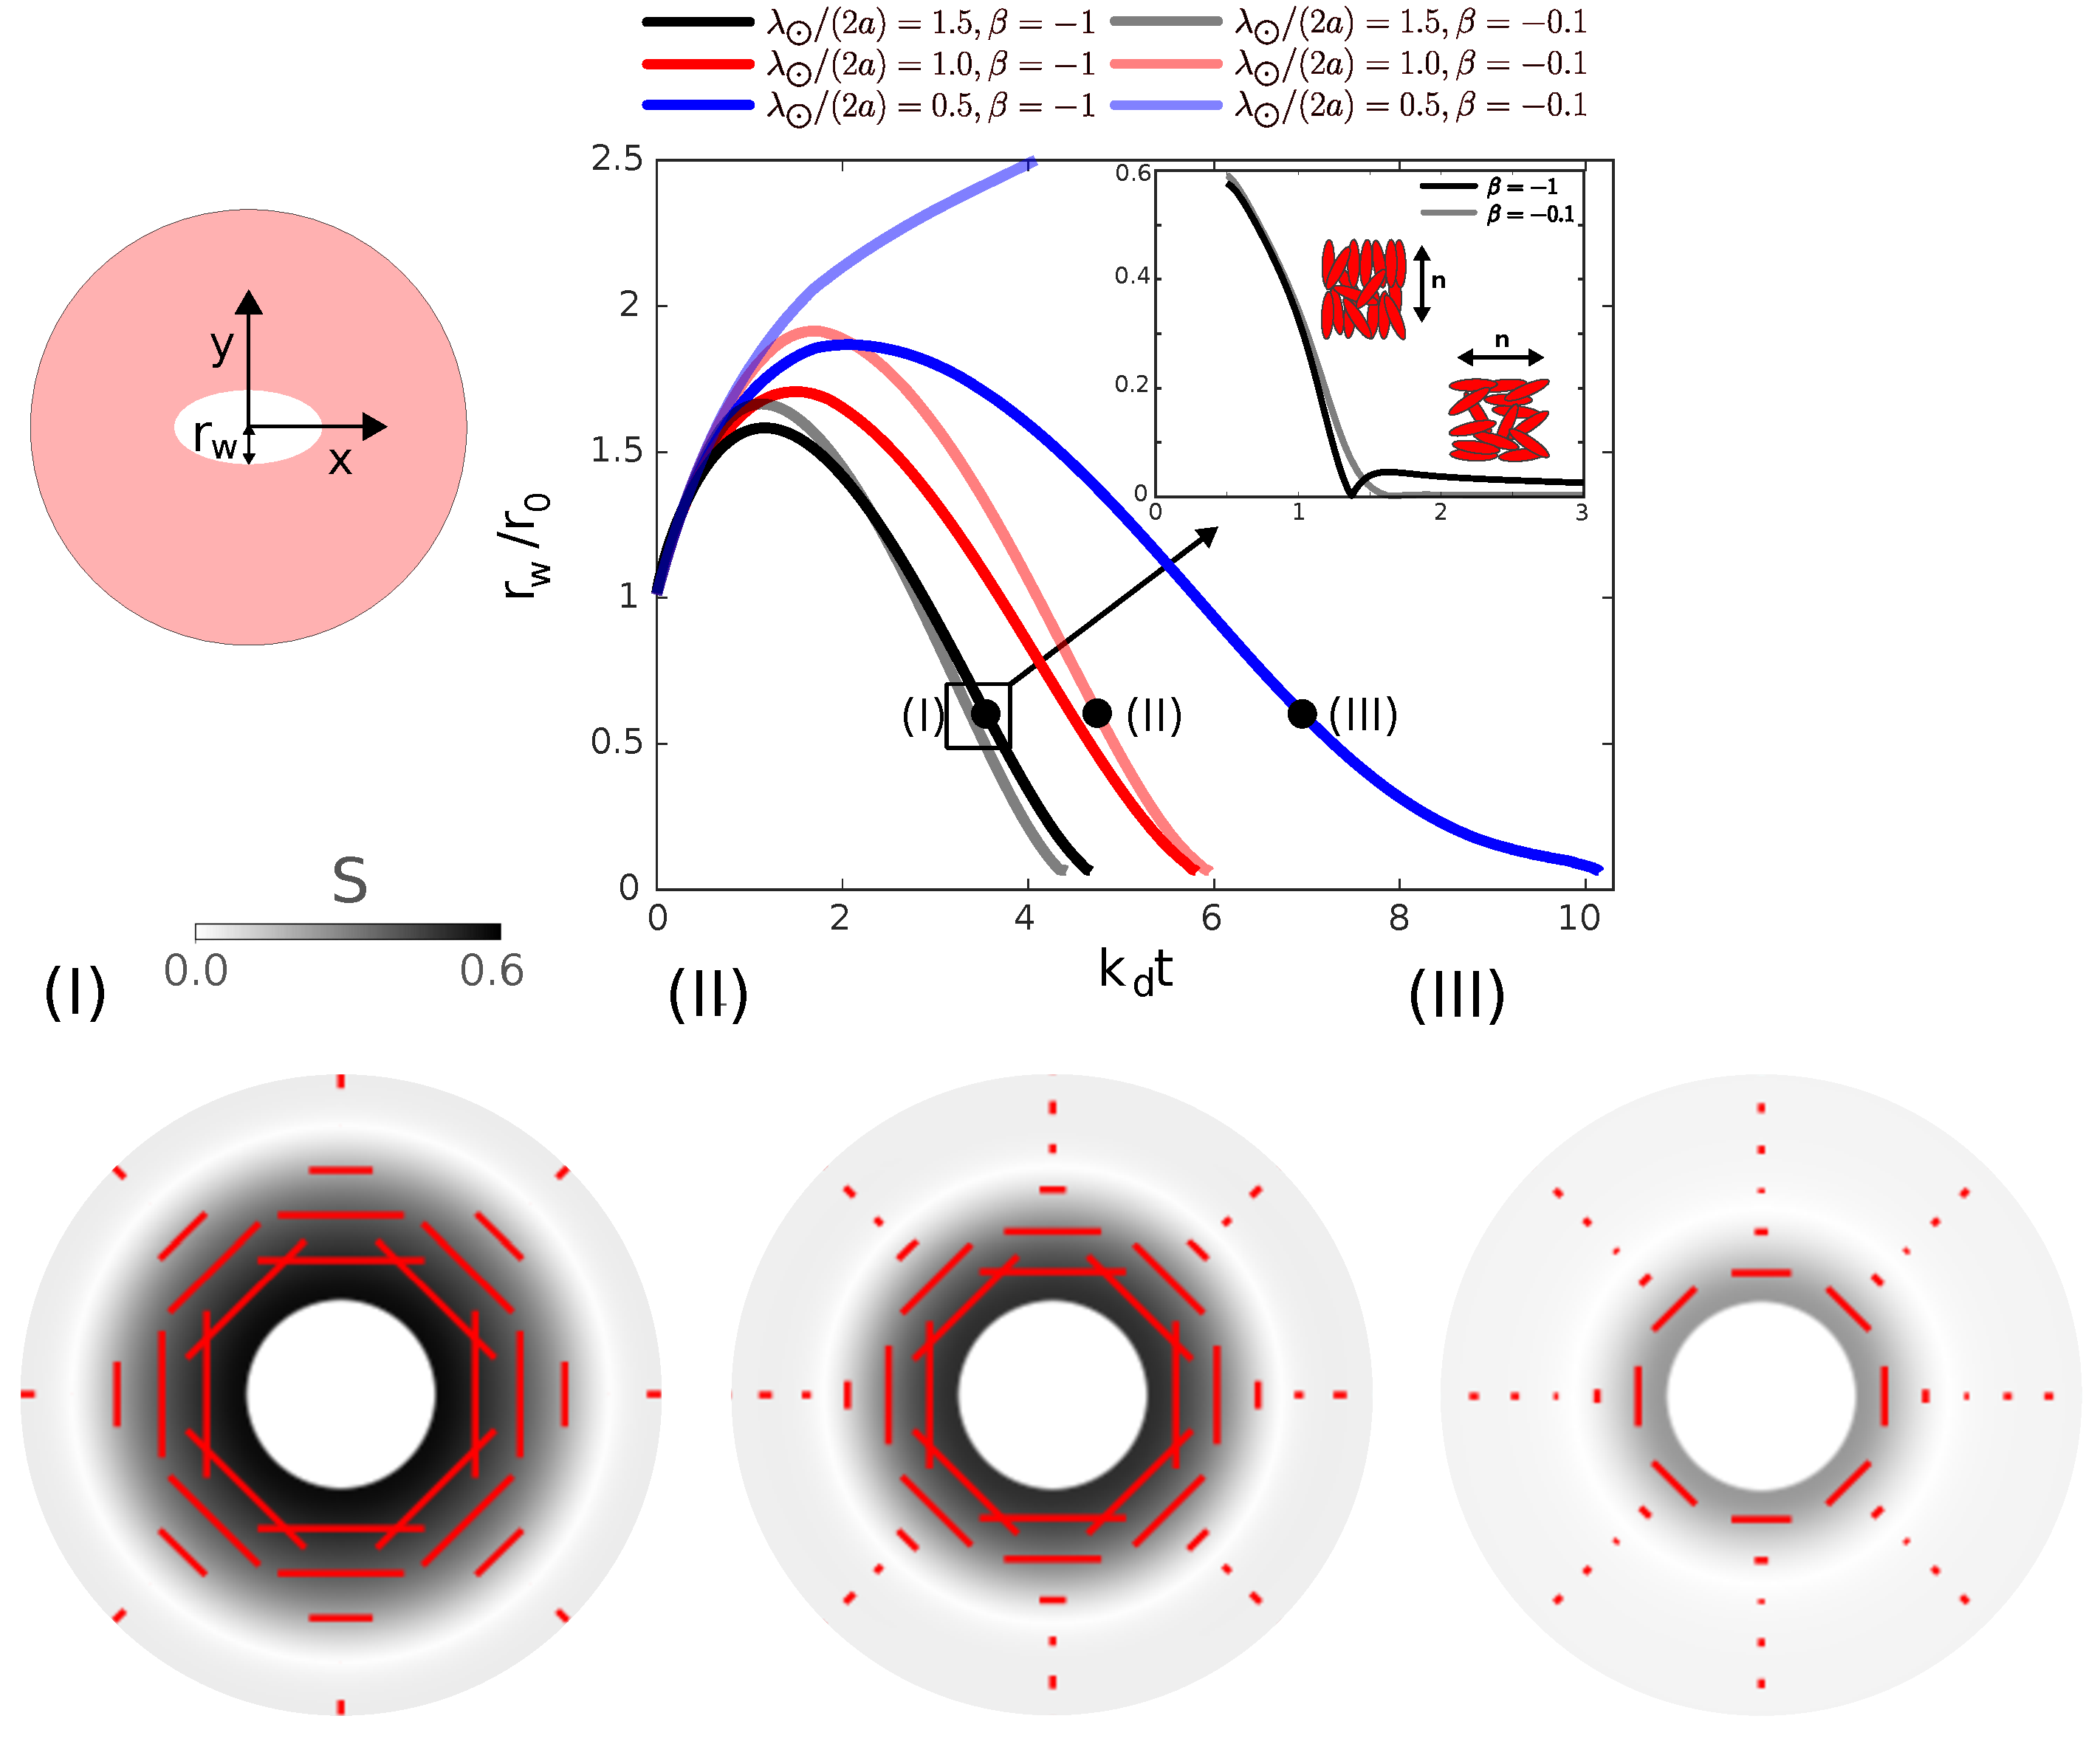
\includegraphics[width=0.85\textwidth]{chap_3_fig_2.pdf}
		\caption{\label{sec_1_chap_3_fig_2}  \textbf{Effect of the flow aligning parameter $\beta$ and nematic activity $\lambda_{\bigodot}$ on the constriction dynamics}. Normalized wound size  $r_w$ as a function of time for different choices of parameters. The snapshots (I-III) show the nematic organization at a given wound size for different $\lambda_{\bigodot}$. Nematic field is represented by a color map for $S$ and by red segments, whose direction indicates the nematic orientation and whose size is proportional to $S$. The size and direction of the red segments indicate the nematic order parameter and average nematic orientation, respectively. }
\end{figure}


\subsection{Defects in a confined colony of spindle-shaped cells}

Elongated spindle-shaped contractile cells such as myoblasts or fibroblasts exhibit long-range nematic order in circular confined dense cultures \cite{duclos2014,guillamat2020} due to their tendency to mutually align parallel with each other \cite{elsdale1968}. Cells confined in these circular domains tend to align parallel or perpendicular to the boundary \cite{guillamat2020}.
Because of this alignment, the net charge of the topological defects in the colony is $+1$, as required by the Poincar\'{e}-Hopf theorem \cite{jubin2009}. This is satisfied by the generation of one or more pairs of topological defects with charge $\pm 1/2$.
%This leads to disruption in the nematic field by self-organization of $\pm 1/2$  topological defects.
Because nematic order controls the anisotropy of active stresses in the cell monolayer, topological defects actively move and may lead to a variety of out-of-equilibrium behaviors. 
Depending on the size of the geometrical confinement with respect to the characteristic lengths of the system, self-organized flows of defects are either absent \cite{duclos2014}, spiral or turbulent-like \cite{norton2018}. 

Here, using the proposed computational framework, we examine the dynamics of a spatially confined dense contractile active nematic system. In this dense cell colony, density variations are arguably small, and hence the density-dependent aspects of our model may not be important. However, we note that an incompressible model for an active liquid crystal may not be pertinent either as convergent/divergent flows are possible due to cell extrusion/proliferation. To simplify the model, we place ourselves in the limit of high turnover rate, for which density is uniform and convergent/divergent flows are allowed. This only leaves us with the coupling between nematic and velocity fields. In order to model the propensity of cells towards mutual alignment, we set the susceptibility parameter such that the initial nematic order is close to $S_0=\sqrt{2|a|/b}=1$. All model parameters are detailed in Table~\ref{modal_parameters}. Furthermore, we impose a boundary condition such that the director field  $\bm{n}|_{\bm{x}=\partial A}$ is fully aligned either tangentially or perpendicularly to the boundary, which corresponds to parallel or homeotropic anchoring  \ref{sec_1_chap_3_fig_3}(a). We enforce that normal velocity to the boundary is zero (impermeable boundary) by using a penalty term in the Rayleighian given as  $\int_{\partial A} K \left|\bm{v} \cdot \bm{N}\right|^2 dl$, where $K$ is the penalty coefficient, but allows cells to slide tangentially along the boundary.

In the first set of tests,  we explore the behavior of a passive nematic system for different ratios of nematic correlation length scale $\ell_p = \sqrt{L/\left(2|a|\right)}$ to the characteristic size of the domain $\ell_0$.  We start with a spatially correlated random initial condition for $\bm{q}$.  Initially, the topological constraints promote a high gradient in nematic orientation which, in turn, nucleate two $+1/2$ defects near the boundary \cite{hardouin2019,giomi2014}. These $+1/2$ defects travel away from the wall into the bulk and reach a quiescent steady-state \cite{giomi2014}. During this process, the system free-energy decreases \ref{sec_1_chap_3_fig_3}(c) and at steady-state, velocities and rate of dissipation vanish. For systems with parallel (homeotropic) boundary conditions, the tips of the $+1/2$ defects point away from (towards) each other (\ref{sec_1_chap_3_fig_3}(b) left inset). The size of the defect cores relative to system size depends on nematic correlation length scale $\ell_p$. As this quantity becomes large, either by increasing the nematic lengthscale or decreasing system size, we expect the two defects to interact and possibly combine into a single $+1$ defect as observed in small-size cell colonies (\ref{sec_1_chap_3_fig_3}(b) right inset). To examine this, we tracked the distance between the two defects, $d$, as a function of  $\ell_p/\ell_0$, finding that beyond a threshold, $d$ abruptly drops close to zero, with configurations resembling vortices or asters depending on boundary conditions, (\ref{sec_1_chap_3_fig_3}(b) right inset). We note, however, than in the absence of activity, $d$ stays finite, and hence the two defects do not strictly become a $+1$ defect, due to the Coulomb repulsion rendering the bound $+1$ defect unstable in absence of activity \cite{thijssen2020, vafa2020}.
\begin{figure}[H]
	\centering
	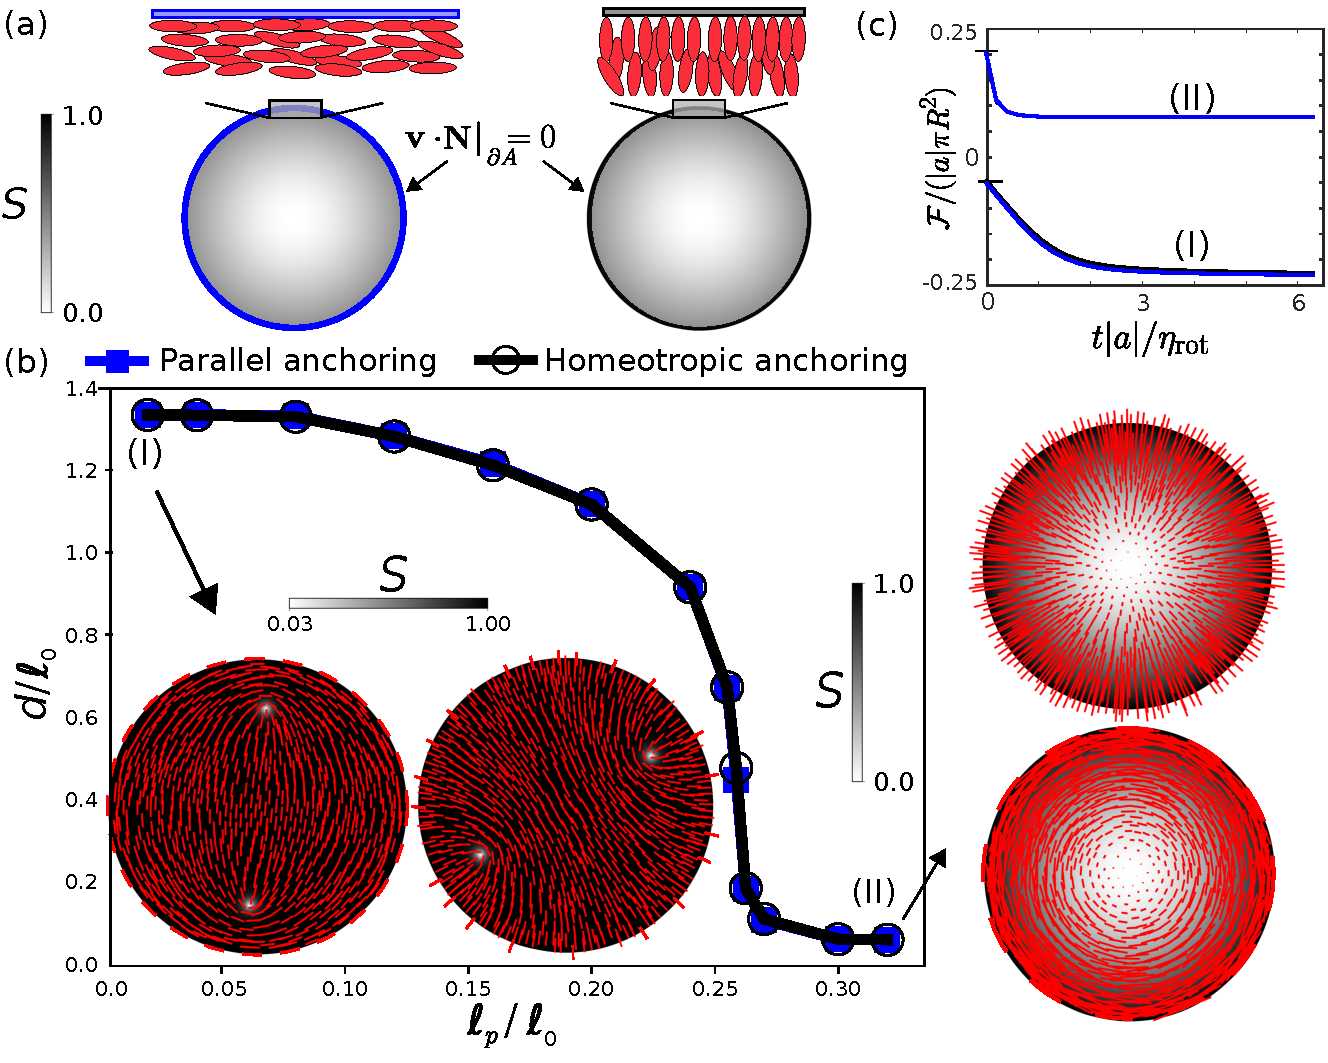
\includegraphics[width=0.75\textwidth]{chap_3_fig_3.pdf}
\caption{\label{sec_1_chap_3_fig_3} \textbf{Effect of nematic correlation length scale $\ell_p$ on the inter-defect distance $d$ in a passive nematic system}. (a) Illustration of nematic and velocity boundary conditions. (b) Inter-defect distance as a function of nematic correlation length scale $\ell_p$ for parallel and homeotropic anchoring conditions, along with selected nematic fields. (c) Monotonically decreasing time-evolution of the Landau free-energy for high and low $\ell_p$ and for both boundary conditions.}
\end{figure}
We next explore the spatiotemporal behavior of defects in a contractile ($\lambda_{\rm aniso} > 0$) active nematic system by examining the  velocity and nematic fields as a function of the active length scale $\ell_a = \sqrt{L/\lambda_{ \rm aniso}}$, given by the ratio of nematic-elastic and active stresses. This active length scale governs fluctuations in both the nematic and velocity fields. We vary this inverse activity parameter at low nematic correlation length scale $\ell_p/\ell_0$ (see Fig.~\ref{sec_1_chap_3_fig_3.5}).  At low activity, we observe that the active contractile stress $\lambda_{\rm aniso} \bm{q}$ leads to new steady-state with a smaller inter-defect distance, Fig.~\ref{sec_1_chap_3_fig_3.5}(b) and left panel of \href{https://github.com/waleedmirzaPhD/movies_thesis.git}{Movie~3.2}, see Appendix~\ref{appendix_3}. More importantly, the steady state of the active system exhibits persistent flows in the nose to tail direction around defects \cite{doostmohammadi2018,ronning2022}, which push these defects by advection of nematic order, Eq.~(\ref{jaumann_detivative_def}). The passive nematic distribution is also distorted slightly by the flow-induced alignment term involving $\beta$.

At a smaller value, $\ell_a/\ell_0 = 0.15$, the two motile $+1/2$ defects move closer together and  towards the wall, with an out-of-equilibrium velocity exhibiting two vortices. After a transient wiggling motion, these to defects stop moving and the system reaches an out-of-equilibrium steady-state,  Fig.~\ref{sec_1_chap_3_fig_3.5}c,d and center panel of \href{https://github.com/waleedmirzaPhD/movies_thesis.git}{Movie~3.2}, see Appendix~\ref{appendix_3}. As we further reduce the ratio $\ell_a/\ell_0$ to $0.1$, the defect distance increases and the two defects rotate in a chiral configuration leading to persistent rotation of the entire system, Fig.~\ref{sec_1_chap_3_fig_3.5}c,d and 
right panel of \href{https://github.com/waleedmirzaPhD/movies_thesis.git}{Movie~3.2}, see Appendix~\ref{appendix_3}. It has been suggested  that the length-scale of such vortex driven by a defect pair is commensurate to $\ell_a$ \cite{chandrakar2020}, and therefore, for lower activity this length-scale is too large for vortices to develop within the domain size. In this regime, the spiral flow suppresses the defect nucleation that might otherwise form through the splay-type hydrodynamic instability \cite{ramaswamy2007, ramaswamy2010}. A similar argument has been made here for bend-type instability for an extensile network of microtubules and  kinesins \cite{opathalage2019}. Upon further lowering the active length scale, $\ell_a/\ell_0 \leq 0.05$ the previously described splay-type hydrodynamic instability emerges \cite{ramaswamy2007, ramaswamy2010}, as shown in Fig.~\ref{sec_1_chap_3_fig_3.5}d (right). In this regime, active stresses overcome the restoring elastic stresses and distort the nematic field to form lines of splay-type disinclination in the bulk and close to the boundary. In turn, these disclination lines destabilize and split into pairs of $\pm 1/2$ defects, which move and annihilate with defects of opposite charge. The persistent generation of disclination lines, their destabilization into point defects, and the motion and annihilation of these defects gives rise to active turbulence, Fig.~\ref{sec_1_chap_3_fig_3.5}(c,d) and  \href{https://github.com/waleedmirzaPhD/movies_thesis.git}{Movie~3.3}, see Appendix~\ref{appendix_3}. At any given time, the system exhibits  more than two defects but the total topological charge is conserved to $+1$.
\begin{figure}[tb]
	\centering
	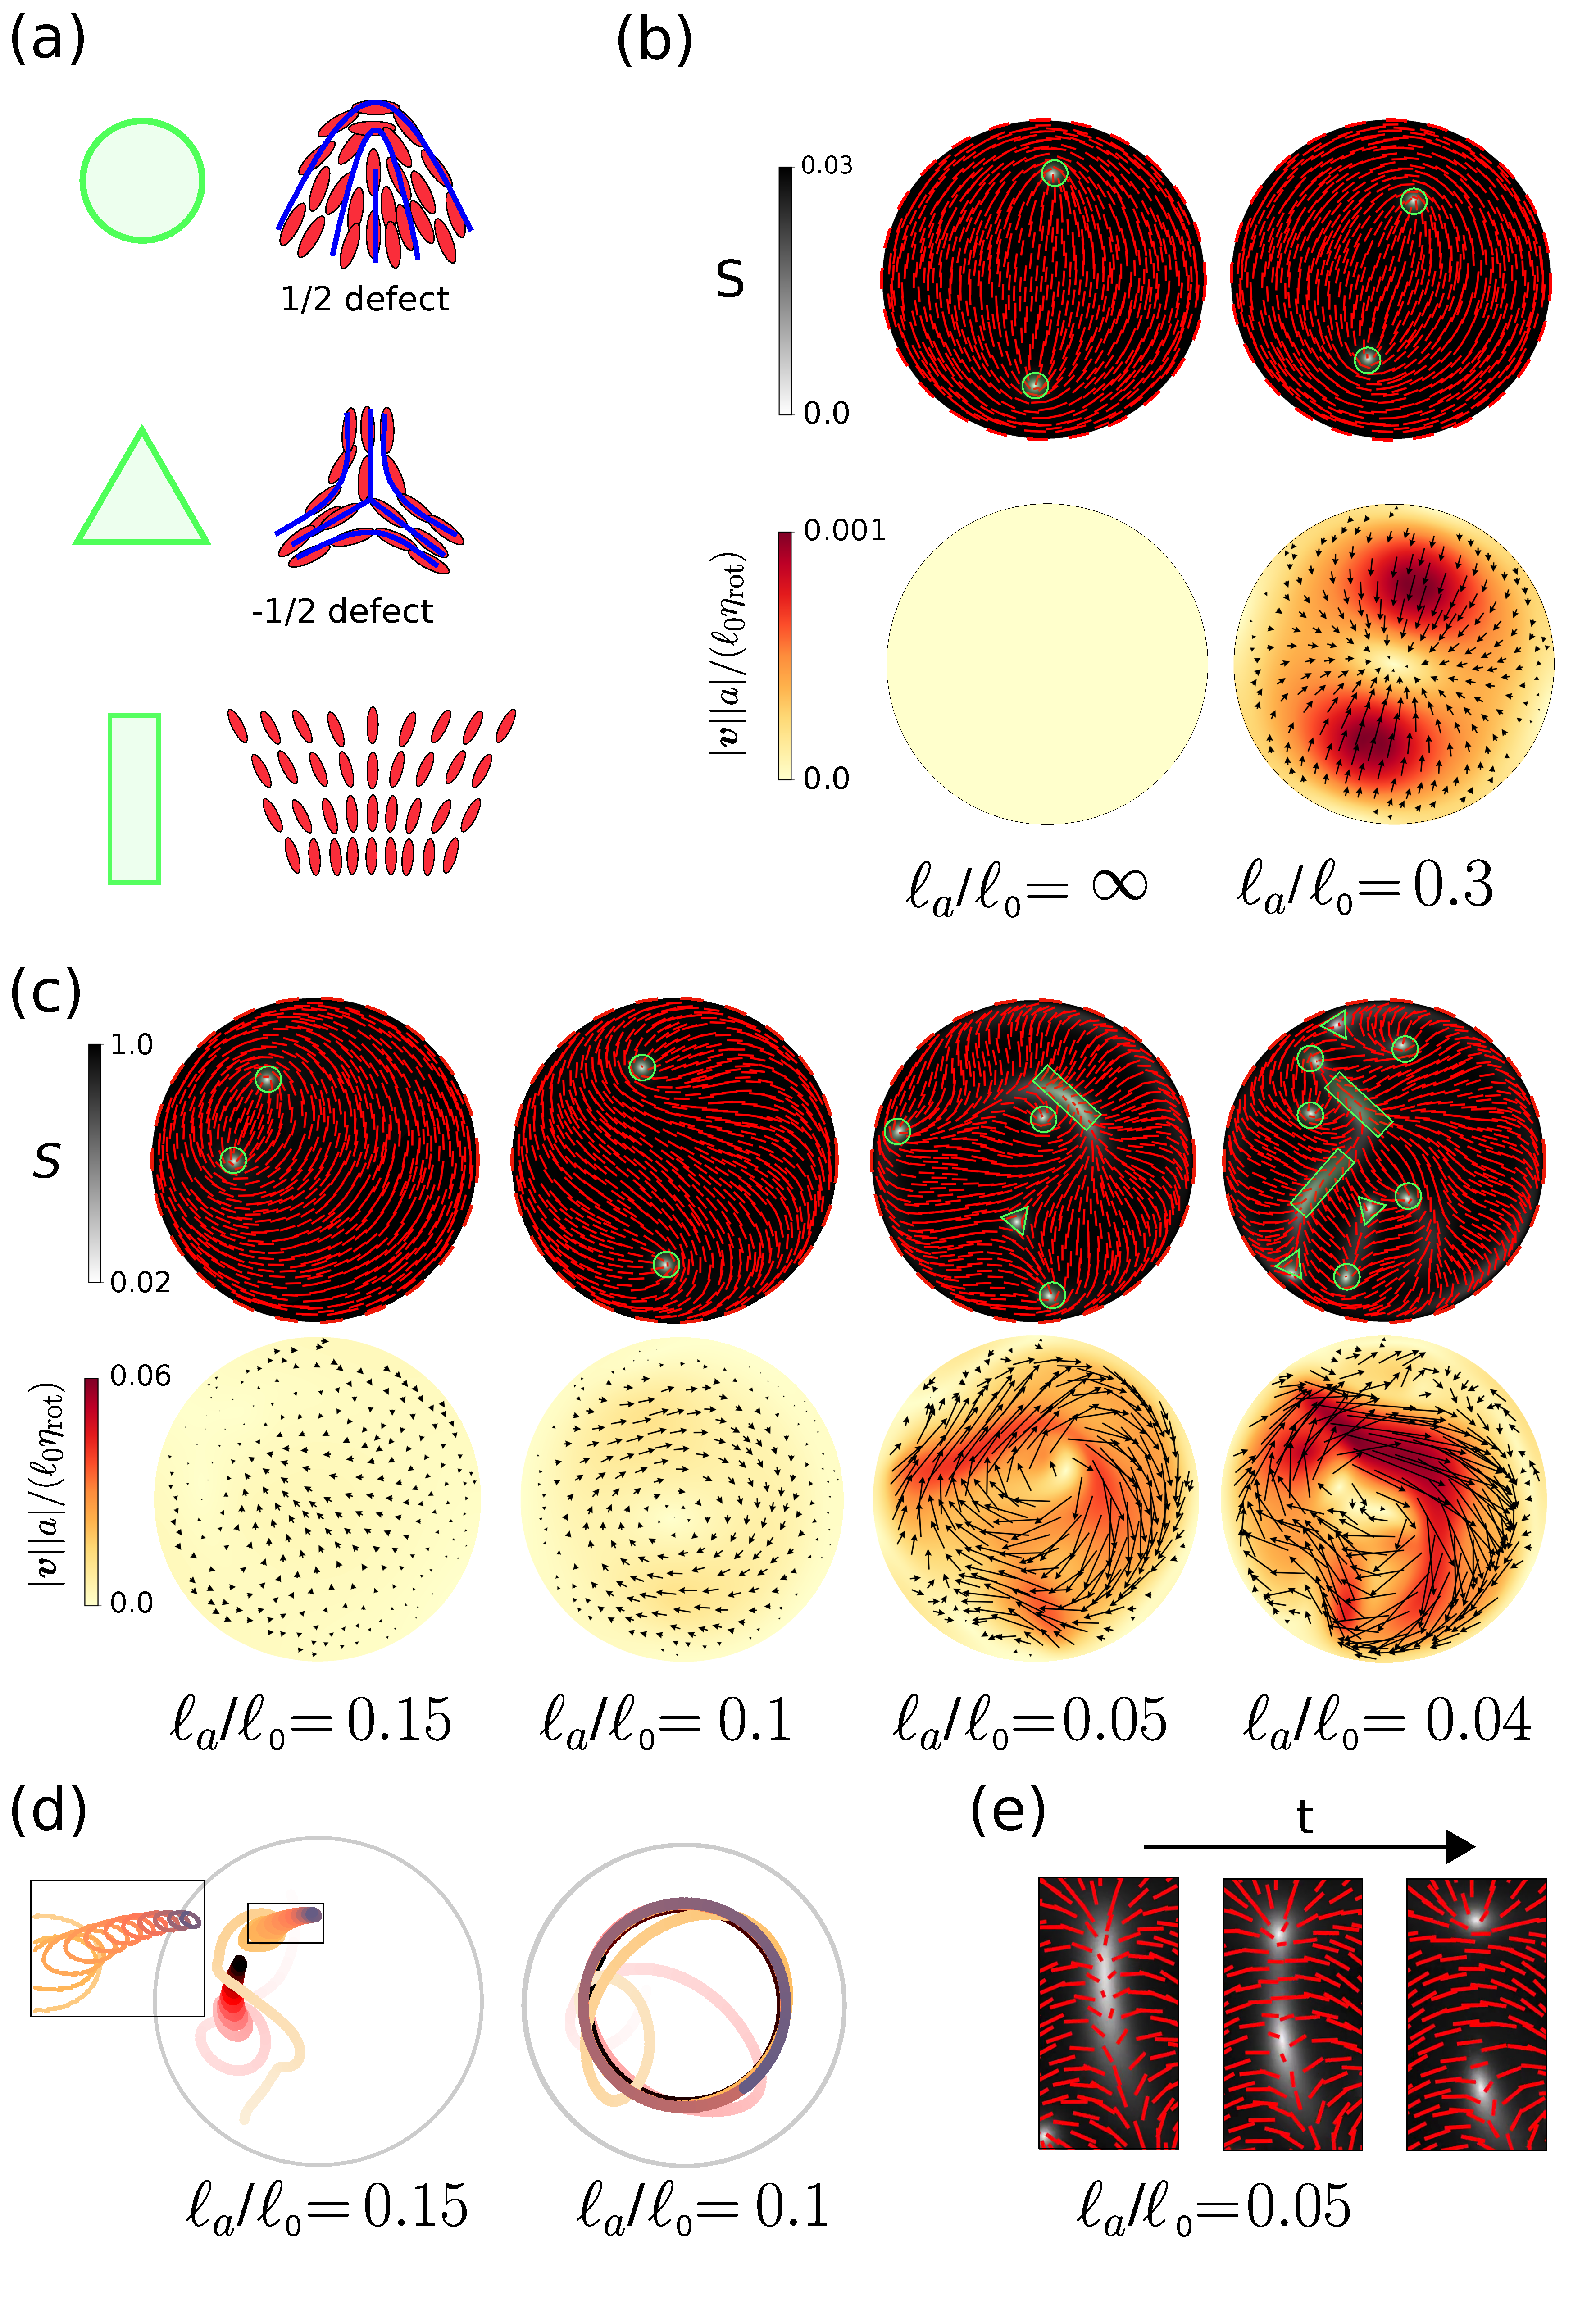
\includegraphics[width=0.62\textwidth]{chap_3_fig_4.pdf}

	\caption{\label{sec_1_chap_3_fig_3.5}  \textbf{Effect of activity on a dense colony of contractile cells under confinement.} (a) Graphical coding of   half integer defects, $\pm \frac{1}{2}$, and of splay bands. (b) Nematic field (top, with segment showing nematic direction and colormap showing order parameter $S$) and velocity and density fields (bottom)  in absence (left) and presence (right) of activity at $\ell_p=0.02$,  \href{https://github.com/waleedmirzaPhD/movies_thesis.git}{Movie~3.2}  (left).	(c) Effect of active nematic length scale on the spatiotemporal distribution of flow, density and nematic fields and $\pm 1/2$ defects at $\ell_p=0.01$,  \href{https://github.com/waleedmirzaPhD/movies_thesis.git}{Movie~3.2}  and \href{https://github.com/waleedmirzaPhD/movies_thesis.git}{Movie~3.3}  (d) Dynamics of the two $+1/2$ defects for $\ell_a/\ell_0=0.15$ and $\ell_a/\ell_0=0.1$. Each defect trajectory becomes darker as time increases. (e) Nucleation of $1/2$ and  $-1/2$ defects from splay bands at $\ell_a/\ell_0=0.05$. }
\end{figure}
In summary, we explored the proposed model in the limit of fast turnover, and hence in the absence of spatio-temporal changes in density, to model a confided cell colony capable of maintaining constant density by rapid division and extrusion. We characterized the passive and active contractile regimes as well as qualitatively compared these behaviors against the literature. In a confided passive nematic system, we observed a canonical spontaneous organization of two $+1/2$ defects with a steady inter-defect distance inversely proportional to the passive nematic length scale $\ell_p  = \sqrt{L/\left(2|a| \right)}$. In the active limit, we observed a diversity of patterns depending on the value of active nematic length-scale $\ell_a= \sqrt{L/\lambda_{\rm aniso}}$.  In general, a gradient in the nematic order in the vicinity of defects generates an active flow, which renders the defects motile. At large values of $\ell_a/\ell_0$, we observe a spiral flow of defects, which turns into a persistent vortical motion in an intermediate range of $\ell_a/\ell_0$. At small values of  $\ell_a/\ell_0$ (high activity), we observe active turbulence in the cell colony characterized by persistent defect nucleation due to splay-type instabilities, motion and annihilation. 

	\section{Summary}


In Chapters~\ref{chap_2} and~\ref{chap_3}, we have proposed a modeling framework for density-dependent active nematic gels based on Onsager's variational formalism. This formalism enables a clear and systematic derivation of otherwise complex equations coupling nematic order, gel velocity and density. We have particularized this framework to develop a specific model, which we have discretized using finite elements and applied to two studies of biological relevance. In the first study, we have explored the role of the self-organization of the actin cytoskeleton during wound repair. We show that a slight overactivity around the wound drives a self-reinforcing flow of the actin network leading to the self-organization of the nematic bundle that efficiently constricts the wound. In a second numerical study, we explore the self-organization of nematic architectures in the limit of high turnover in a constrained colony of contractile cells. Depending on the magnitude of the activity, the topological defects required by boundary conditions either reach a steady state or exhibit highly dynamical flows as well as active turbulence.

%Our framework provides a basis to explore a large variety of active nematic systems. Although here we have focused on simple cases where the nematic architectures are self-organized in a contractile network due to slight overactivity of myosin in the cytoskeleton or due to boundary conditions in a colony of contractile cells, our framework can be applied to understand the diversity of nematic architectures in actomyosin networks \cite{mirza2022}, including bundles  \cite{tojkander2015,jalal2019, vignaud2021}, asters \cite{xia2019}, and tactoids \cite{weirich2017,weirich2019}. If suitably extended to curved and time-evolving surface domains \cite{mirza2023}, the framework presented here can help us examine the interaction between nematodynamics and reshaping during cytokinesis \cite{mayer2010} or hydra morphogenesis \cite{maroudas2021}.


\newpage


\renewcommand{\thesection}{4.\arabic{section}}
\chapter{Theory of active self-organization of dense nematic structures in actin gels} \label{chap_4}
\section{Introduction}

	Actin networks are remarkably dynamic and versatile and organize in a variety of cytoskeletal architectures to accomplish crucial cellular functions \cite{Banerjee2020}. For instance, isotropic thin actin gels form the cell cortex, which largely determines cell shape \cite{chugh2018} and motility in confined non-adherent environments \cite{blaser2006, Ruprecht:2015aa}. Polar structures at the edge of adherent cells, either forming filaments as in filopodia or sheets as in lamellipodia \cite{blanchoin2014}, enable cells to probe their environment and crawl on substrates. Nematic actin bundles, formed by anti-parallel fibers, conform a variety of contractile structures \cite{schwayer2016}, including the cytokinetic ring \cite{anne2016}, supra-cellular rings during wound healing \cite{martin1992} or development \cite{Krieg:2008aa}, subcellular bundle networks during cellularization \cite{dudin2019}, or stress fibers \cite{10.1242/jcs.236604,tojkander2012, tojkander2015}. Nematic bundles consist of highly aligned and densely packed actin filaments of mixed polarity inter-woven by a diversity of cross-linkers and whose assembly and maintenance depends on actin nucleators and regulators \cite{tojkander2012,blanchoin2014,schwayer2016,chugh2018,Banerjee2020}. Observations in cells and reconstituted systems show the essential role of myosin activity and of crosslinking proteins in the formation and maintenance of actin bundles \cite{chrzanowska1996, thoresen2011,strehle2011,laporte2012,chugh2018,lehtimaki2021}.
	
	Several studies emphasize the morphological, mechanical, dynamical, molecular and functional specificities of each of the families of actin bundles such as dorsal, transverse, and ventral stress fibers or contractile rings \cite{hotulainen2006,naumanen2008,tojkander2012,tojkander2015,doi:10.1091/mbc.E18-02-0106}. Nevertheless, observations across cell types also suggest that these nematic strands emerge as a result of self-organization of the active actomyosin gel. Suggestive of such an active self-organization, nematic fibers often form patterns with regular spacing, sometimes with families of fibers along orthogonal directions  \cite{tee2015, tojkander2015,wirshing2017, yolland2019, jalal2019,10.1242/jcs.236604}, dynamically fuse \cite{hotulainen2006,wirshing2017} and form a mechanically coherent network with the isotropic cortical network \cite{vignaud2021,lehtimaki2021}. Despite the self-organization of the actin cytoskeleton has been examined with active gel models in various contexts \cite{callan2013,kruse2004,hannezo2015},
	%, such as cell polarization \cite{callan2013}, the formation of asters \cite{kruse2004} or supracellular rings \cite{hannezo2015}, 
	the active self-organization of dense aligned nematic fibers and their dynamical interplay with a low-density, isotropic background network is not understood.

	To test the idea of physical self-organization of such nematic bundles, we develop here an active gel model accounting for nematic order in the spirit of \cite{salbreux2009,anne2016,julicher2018}. In agreement with the fact that nematic bundles require contractile activity, the transition from isotropic to nematic states is driven by active power input rather than by a more conventional density-dependent mechanism \cite{e2011}. Using linear stability analysis of the dynamical equations, we identify a distinct mechanism of pattern formation coupling density and nematic order variations. We further examine the fully nonlinear regime through numerical simulations, which establish the conditions for the self organization of an initially isotropic and uniform actin gel into dense nematic bundles and establish how key non-dimensional parameters affect the geometry and dynamics of bundle networks. Finally, we test the two key requirements for dense nematic bundle self-organization, namely the existence of active tension anisotropy and active forces conjugate to nematic order, using discrete network simulations. 	
    \begin{figure}[H]
		\centering
		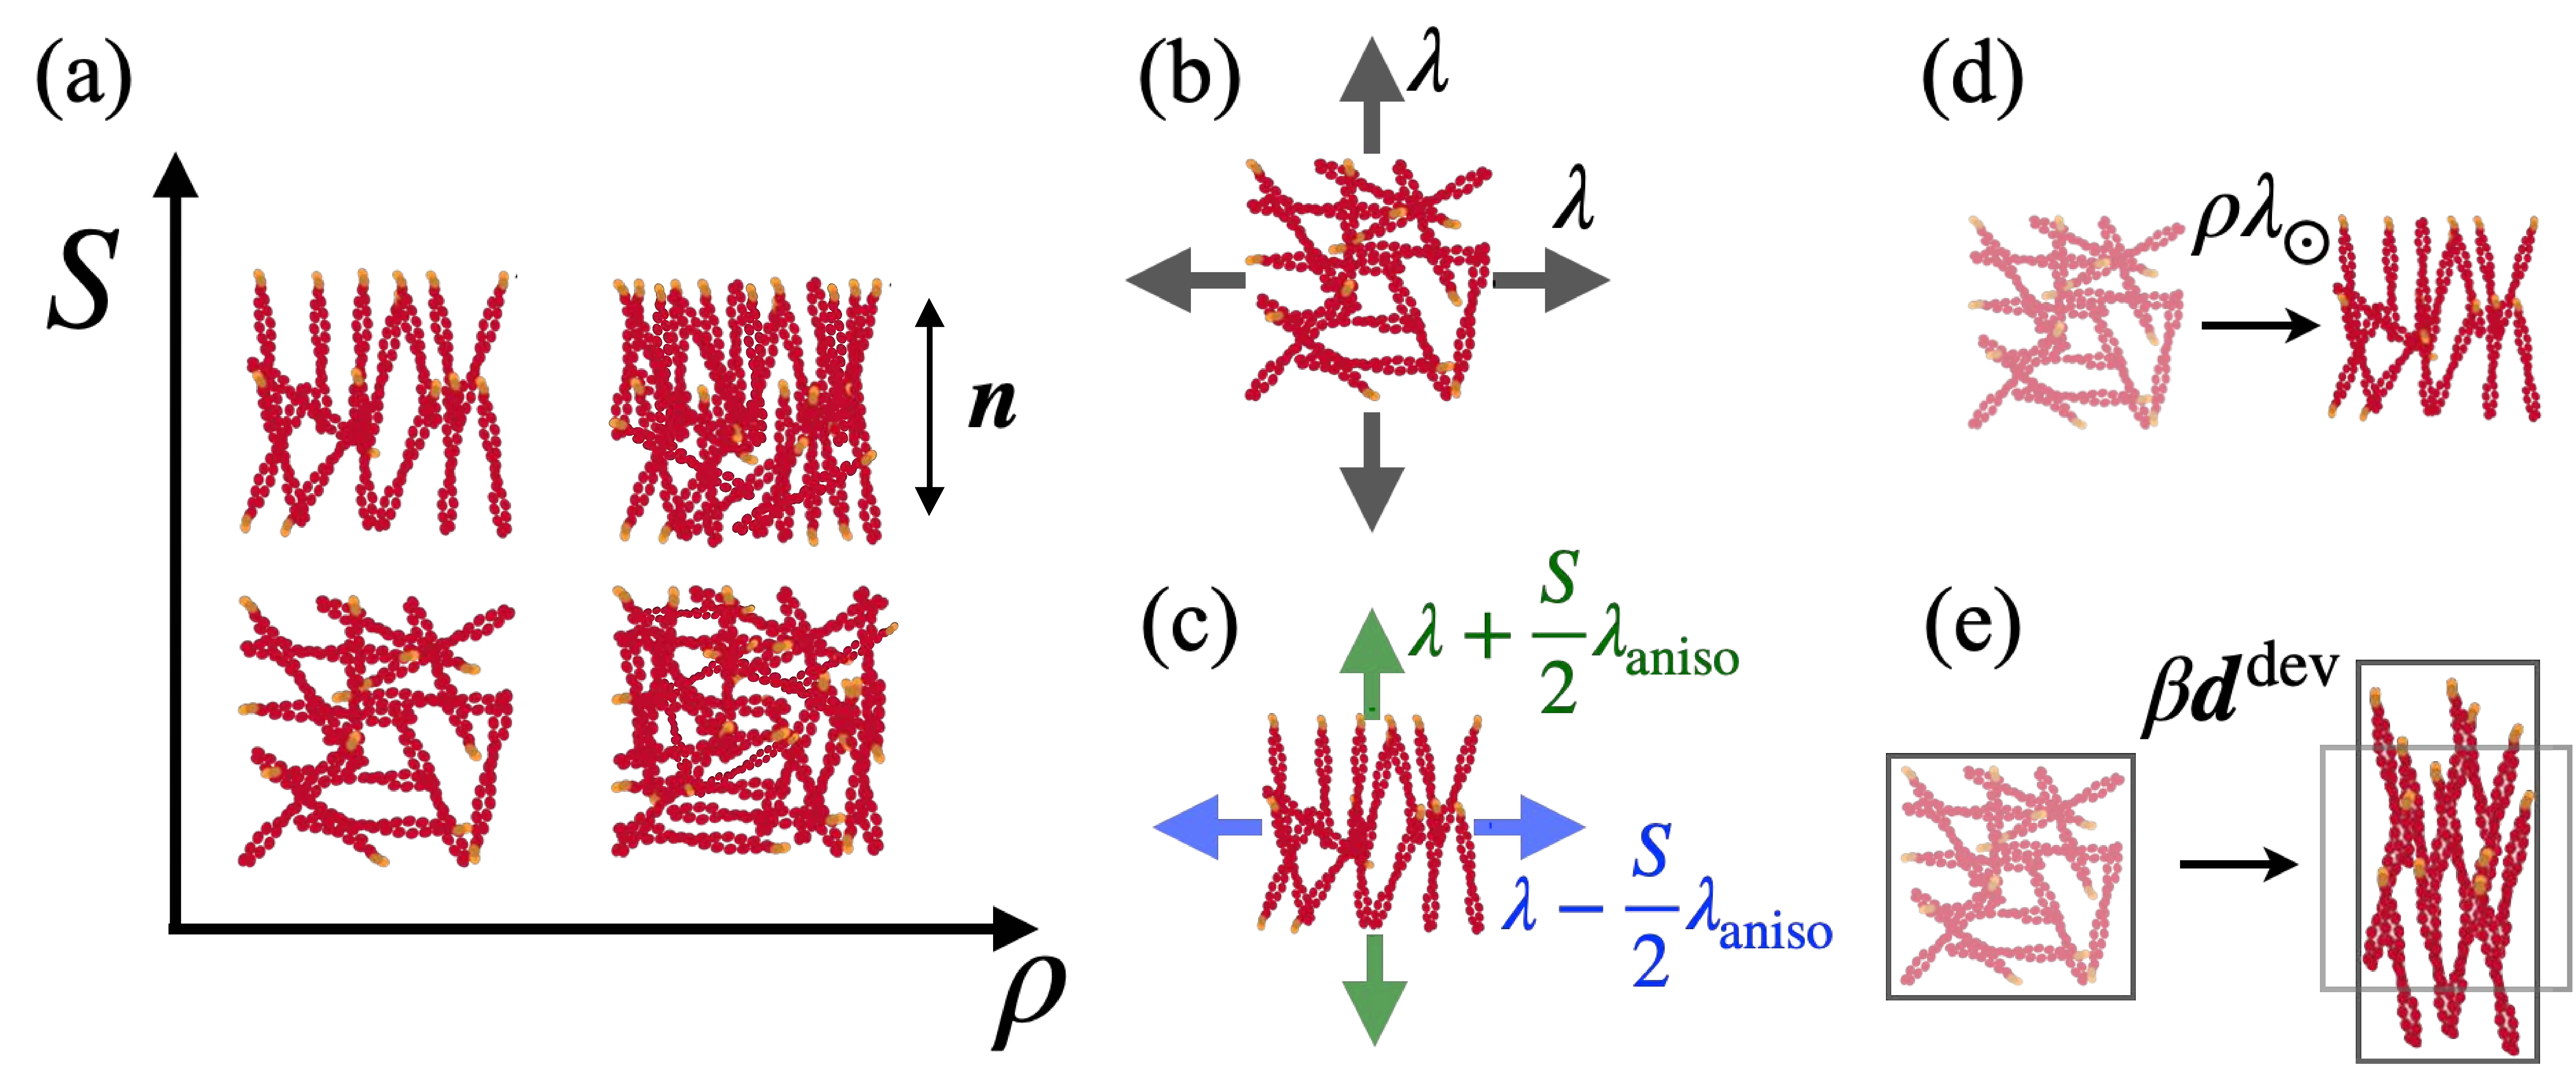
\includegraphics[width=0.7 \textwidth]{Figure_1.png}
		\caption{{\bf Key model ingredients}. (a) The local state of the system is defined by its density $\rho$ and by its orientational order quantified by the nematic parameter $S$ and by the nematic direction $\bm{n}$.  (b) Active tension is isotropic and given by parameter $\lambda$ when the network is isotropic ($S=0$), and (c) becomes anisotropic as $S$ increases as controlled by non-dimensional parameter $\kappa = \lambda_{\rm aniso}/\lambda$. Orientational order is driven by (d) active forces conjugate $S$ and characterized by parameter $\lambda_{\odot}$ and by (e) passive flow-induced alignment in the presence of deviatoric rate-of-deformation with coupling parameter $\beta$.}
		\label{fig4.1}
	\end{figure} 

	\section{Results}
	\noindent{\bf Theoretical model.}	As a coarse-grained description of a thin layer actin cytoskeleton, as in the cortex, we consider a nematic active gel in 2D. A number of active cellular and cytoskeletal systems have been modeled using nematic active liquid-crystal theory, including dense colonies of elongated cells or dense confined cytoskeletal gels \cite{giomi2014,duclos2017,kumar2018}. In such systems, crowding forces strong nematic order everywhere except at defects, which are generated by activity or required by topology. We argue that the porous actin cytoskeleton is not a nematic active liquid-crystal because it can adopt extended isotropic or low-order phases, and hence defects are not topologically required. Furthermore, the main mechanism driving nematic order is active contractility \cite{hotulainen2006}. Finally, liquid crystals are crowded and hence nearly incompressible, whereas actin gels develop large density variations.  We thus formulate an active gel model capable of accommodating large density variations and where nematic ordering is actively driven. 
	
	 At a given time $t$, the state of the system is described by the areal density of cytoskeletal material $\rho$ and by the network architecture quantified by the nematic order tensor $\bm{q}$, see Fig.~\ref{fig4.1}a. Assuming a fixed volumetric density $\rho_{\rm vol}$, $\rho$ can be interpreted as a cytoskeletal thickness $\rho/\rho_{\rm vol}$. The nematic tensor can be expressed as  $q_{ij} =S\left({n}_i n_j - \delta_{ij}/2 \right)$, where $\bm{n}$ is the average molecular alignment and $S=\sqrt{2   q_{ij}q_{ij}}$ the degree of local alignment about $\bm{n}$. We denote by $\bm{v}( \bm{x},t )$ the velocity field of the gel and by $\bm{d} = \frac{1}{2}(\nabla \bm{v}+ \nabla \bm{v}^T)$ and $\bm{w} = \frac{1}{2}(\nabla \bm{v}- \nabla \bm{v}^T)$ the rate-of-deformation and spin tensors. The rate of change of $\bm{q}$ relative to a frame that translates and locally rotates with the flow generated by $\bm{v}$ is given by the Jaumann derivative $\hat{\bm{q}} = \partial \bm{q} /\partial t + \bm{v} \cdot \nabla \bm{q}- \bm{w} \cdot \bm{q} +  \bm{q} \cdot \bm{w}$ \cite{de1993}.

Based on Onsager's variational formalism \cite{doi2011,arroyo2018}, we systematically derive the governing equations as detailed in Chapter~\ref{chap_2} and summarized next. According to this formalism, the dynamical equations of the active gel result from a competition between nematic free-energy release, dissipation and active power input subjected to mass balance. Because we consider a bi-periodic domain, we ignore here explicit boundary terms. 

Transport and turnover of the cortical material is described by 
\begin{equation} \label{eq_thick}
	\frac{\partial \rho }{\partial t} + \bm{\nabla} \cdot \left ( \rho \bm{v} \right) - D \Delta \rho + k_d(\rho-\rho_0)=0,
\end{equation}
where $D$ is an effective diffusivity, $\rho_0$ is the steady-state areal density and $k_d$ is the depolymerization rate. Balance of linear momentum takes the form
\begin{equation} \label{eq_lin_mom}
	\rho \gamma \bm{v} = \bm{\nabla} \cdot \bm{\sigma},
\end{equation}
where $\gamma>0$ models friction with a background medium and  $\bm{\sigma}$ is the Cauchy stress tensor, which in 2D has units of tension. We split it into symmetric and antisymmetric components as $\bm{\sigma} = \bm{\sigma}^{\rm s} + \bm{\sigma}^{\rm a}$. The symmetric component is given by
\begin{align}
	{\sigma}^{\rm s}_{ij} = & \rho \bigg\{  2\eta \left[ d_{ij} + d_{kk} \delta_{ij}\right]+ \beta  \hat{{q}}_{ij}  + {\sigma}^{\rm act}_{ij} - L q_{kl,i} q_{kl,j}  \bigg\},  \label{symm_stress} 
\end{align}
where $L>0$ is the Frank constant, $\eta>0$ is the shear viscosity, $\beta<0$ measures the dissipative coupling between nematic order and strain rate \cite{anne2016}, which here induces a stress proportional to changes in nematic tensor, and  ${\sigma}^{\rm act}_{ij}$ is the active tension resulting from expenditure of chemical energy in the gel. To model the dependence of contractility on network architecture \cite{Ennomani2016}, we assume ${\sigma}^{\rm act}_{ij} = \lambda \delta_{ij} + \lambda_{\rm aniso} q_{ij} = \lambda \left( \delta_{ij}  + \kappa q_{ij} \right)$ where $\kappa = \lambda_{\rm aniso}/\lambda$ measures the sign and strength of active tension anisotropy. When order is low ($S\approx 0$), active tension is isotropic, Fig.~\ref{fig4.1}b, whereas when order is high, active tension becomes anisotropic, Fig.~\ref{fig4.1}c, with active tension along the nematic direction reflecting the sliding of antiparallel fibers driven by myosin motors, and perpendicular to it reflecting the the out-of-equilibrium binding of bundling proteins or myosins \cite{harris2006,courson2010,blanchoin2014,schuppler2016,li2017,nandi2018,Ennomani2016,chen2020}. The antisymmetric part of the Cauchy stress, derived from balance of angular momentum, is purely elastic-nematic and given by ${\sigma}^{\rm a}_{ij} =  L \nabla_l \rho \left( \nabla_l q_{kj} q_{ik} - \nabla_l q_{ki} q_{jk} \right) + \rho L  \left( q_{ik}\Delta q_{jk}  -q_{jk}  \Delta q_{ik}  \right)$.

Balance of the generalized forces power-conjugate to $\hat{\bm{q}}$ also includes viscous, elastic-nematic and active contributions, and takes the form  
\begin{equation} \label{eq_nemat}
	\eta_{\text{rot}} \hat{\bm{q}} + \beta \bm{d}^{\rm dev} + (2a + b S^2)  \bm{q} - L \Delta \bm{q} - L  \nabla\bm{q} \cdot \frac{\nabla \rho}{\rho} - \rho \lambda_{\bigodot} \bm{q} = 0,
\end{equation}
where $\eta_{\text{rot}}$ is a nematic viscous coefficient, the second term models alignment induced by strain rate (Fig.~\ref{fig4.1}e) with the deviatoric part of the rate-of-deformation tensor given by $\bm{d}^{\rm dev} = \bm{d} - ({\rm tr}\,\bm{d}/2) \bm{I}$, and $a>0$ and $b>0$ are susceptibility coefficients. The last term is an active generalized force controlled by activity parameter $\lambda_{\odot}\ge 0$  tending to further align filaments (Fig.~\ref{fig4.1}d) \cite{anne2016}. This term is linear in $\rho$ because in the expansion $\bar{\lambda}_{\odot} + \rho \lambda_{\odot}$ the constant contribution $\bar{\lambda}_{\odot}$ can be subsumed by the susceptibility parameter $a$. Thus, the active term acts as a negative density-dependent susceptibility. When $c_0 =2a - \rho_0 \lambda_{\odot}<0$, the system can sustain a uniform quiescent state with $\rho(\bm{x},t) = \rho_0$, $\bm{v}(\bm{x},t) = 0$ and a  non-zero nematic tensor satisfying $S^2 = -c_0/b$. Even if $c_0>0$ and hence the uniform quiescent state is devoid of order,  pattern formation can induce density variations such that $2a - \rho \lambda_{\odot}$ becomes locally negative and actively favors local nematic order. The dissipative parameters in the model are constrained by Onsager's inequality, $2\eta \, \eta_{\text{rot}} - \beta^2 \geq 0$ (see Section~\ref{inequality}), which guarantees positive dissipation \cite{Onsager1931}.

By freezing an isotropic state, $S=0$, our model reduces to an orientation-independent active gel model, which develops periodic out-of-equilibrium patterns driven by self-reinforcing active flows sustained by turnover \cite{hannezo2015}. However, here the dynamics of orientational order, Eq.~(\ref{eq_nemat}), are coupled to the translational and density dynamics, Eqs.~(\ref{eq_thick},\ref{eq_lin_mom}), through $\beta$ and the term involving $\rho \lambda_{\odot}$, and conversely translational  dynamics, Eq.~(\ref{eq_lin_mom}), directly affect density dynamics, Eq.~(\ref{eq_thick}),  through $\bm{v}$ and depend on nematic order through the contributions to the stress tensor depending on $\kappa$, $\beta$ and $L$, Eq.~(\ref{symm_stress}). Hence, order affects translational and density dynamics. 

We readily identify the hydrodynamic length $\ell_s =\sqrt{\eta/\gamma}$, above which friction dominates over viscosity, the Damk\"olher length $\ell_D =\sqrt{D/k_d}$ above which reactions dominate over diffusion, and the nematic length $\ell_q=\sqrt{L/ \left | 2a - \lambda_{\odot} \, \rho_0 \right |}$. Non-dimensional analysis (see Section~\ref{appendix_1_sec_5}) reveals a set of non-dimensional groups that control the system behavior, namely the non-dimensional turnover rate $\bar{k}_d = \ell_s^2/\ell_D^2$, the  Frank constant $\bar{L} = L/(\eta D)$, the susceptibility parameters $\bar{a} = a/(\gamma D) and \bar{b} = b/(\gamma D)$, the drag coefficients $\bar{\eta}_{\rm rot} = {\eta}_{\rm rot}/\eta$ and $\bar{\beta} = \beta /\eta$, the nematic activity coefficient $\bar{\lambda}_\odot=\rho_0 \lambda_\odot / (\gamma D)$, and the active tension parameters $\bar{\lambda} = \lambda / (\gamma D)$ and $\kappa$.  The full list of material parameters for each figure and movie is given in Tables~\ref{defaulttable},~A.3 and justified in Section~\ref{appendix_1_sec_7}.


\medskip
\noindent{\bf Onset and nature of pattern formation.} To examine the role of nematic order in the emergence of various actin architectures, we performed linear stability analysis of our model particularized to 1D , see Sections~\ref{appendix_1_sec_4} and~\ref{appendix_1_sec_6}. The variables of the model are flow field along the $x-$direction $v(x,t)$, $\rho(x,t)$, and $q(x,t)$, where  $q>0\;(<0)$ corresponds to a nematic  orientation $\bm{n}$ parallel (perpendicular) to the $x-$axis. We first focused on the case $c_0=2a - \rho_0 \lambda_{\odot}>0$ to examine the loss of stability of a uniform, isotropic, and quiescent steady state ($\rho(x,t) = \rho_0$, $v(x,t) = 0$, $q(x,t)=0$) by increasing the master activity parameter $\lambda$ and identifying the most unstable modes. This allowed us to determine a threshold activity for pattern formation and the wavelength of the emerging pattern. Since the exact evaluation of such quantities requires solving nonlinear equations, we derived explicit expansions in the limit of small $L$ for the critical contractile activity 
\begin{align}
	\lambda_{\rm crit} \approx \lambda_{\rm crit,0} \left[1 - \frac{1}{2}\frac{\ell_s}{\ell_D}\left(1+  2\frac{\ell_s}{\ell_D}\right) \delta \right] + \mathcal{O}(\delta^2)
	\label{lam_c}
\end{align}
where $\lambda_{\rm crit,0} = (\sqrt{\gamma D} + 2 \sqrt{k_d\eta})^2 = \gamma D (1+2\sqrt{\ell_s/\ell_D})^2$ and $\delta = \gamma D \kappa \beta /(2\eta c_0)$, 
and for the the corresponding wavenumber
\begin{align}
	\nu_{\rm crit}^2 \approx \nu_{\rm crit,0}^2\left[1 + \frac{1}{8}\left(1 +  2\frac{\ell_s}{\ell_D}\right)^2 \delta \right] + \mathcal{O}(\delta^2), \label{nu_c}
\end{align}
where $\nu_{\rm crit,0}^2 = \left[k_d \gamma /(4\eta D)\right]^{1/2} = 1/({2\ell_s\ell_D})$. 

	
\begin{figure}
	\centering
	\includegraphics[width=0.9\textwidth]{Figure_2.pdf}
	\caption{{\bf Active formation of patterns coupling nematic order and density maintained by self-reinforcing flows and turnover.} (a) Dimensionless order parameter characterizing relative orientation of nematic direction and high-density bands defined by $\omega = {\ell_s^2}/{(\rho_0^2\vert A\vert)}\int_A \nabla\rho\cdot \boldsymbol{q} \nabla\rho~dS$ as a function of active tension anisotropy parameter $\kappa$, showing transition from states with nematic direction parallel to high-density structures ($\omega<0$), which we call fibrillar patterns, for $\kappa<0$ to states with nematic direction perpendicular to high-density structures  ($\omega>0$), which we call sarcomeric patterns, for $\kappa>0$. (b) Map of density, nematic order $S$, nematic direction (red segments) and flow field (green arrows) for quasi-steady fibrillar (I), sarcomeric (III) patterns, and for a transition pattern of high density droplets with high nematic order (II) corresponding to isotropic active tension (small $\kappa$). (c) These quasi-steady states are out-of-equilibrium and maintained by self-reinforcing flows and turnover.}
	\label{fig4.2}
\end{figure} 



When  $\kappa = 0$ or $\beta =0$, and hence $\delta = 0$, we recover the predictions of an active gel model not accounting for network architecture \cite{hannezo2015}, $\lambda_{\rm crit} = \lambda_{\rm crit,0}$ and $\nu_{\rm crit} = \nu_{\rm crit,0}$. However,  active tension anisotropy ($\kappa \ne 0$) and flow-induced alignment ($\beta <0$) fundamentally change the nature of pattern formation. Nematic order introduces  quantitative changes in critical tension and wavenumber, which depend on the ratio of hydrodynamic and Damk\"olher lengths and on the strength and sign of nematic coupling and can be very significant depending on the parameter regime. The nematic corrections increase as $c_0 \rightarrow 0$, close to the point where the uniform quiescent state develops spontaneous order. We thus studied separately the regime $0<c_0 \ll 1$ (details in Section~\ref{appendix_1_sec_6}), finding analogous expansions for the critical tension and wavenumber in terms of $\delta = \gamma D \kappa \beta /(2\eta L)$. Interestingly, Eq.~(\ref{lam_c}) shows that the activity threshold is reduced, and hence pattern formation facilitated, when $\kappa<0$, i.e. when active tension is larger perpendicular to the nematic direction. Besides these quantitative changes in critical tension and wavenumber, the present model predicts that the dynamical modes with self-reinforcing flows create patterns where high density co-localizes with high nematic order.
%\MAB{Our analysis predicts that the sign of $q(x,t)$ in regions of high density coincides with that of $\kappa$, i.e.~filaments align along/perpendicular to the $x-$direction when active tension is larger along/perpendicular to the nematic direction. [Please check this]}



To test the validity of this analysis and further understand the system beyond the onset of pattern formation, we performed fully non-linear finite element simulations (see Chapter~\ref{chap_3}) in a periodic 2D domain. In these simulations, we increased the activity parameter $\lambda$ beyond the instability starting from a quiescent uniform state. We found that the linear stability analysis very accurately predicts the activity thresholds and pattern wave-numbers within two percent across a wide range of parameters. In the nonlinear regime, the exponentially-growing instabilities eventually reach out-of-equilibrium quasi-steady-state patterns maintained by turnover and by self-reinforcing flows towards regularly-spaced regions of high density surrounded by a low density matrix. 

In the absence of nematic coupling ($\beta = \kappa = \lambda_\odot = 0$), these high density domains are droplets arranged in a regular hexagonal lattice with $S=0$ throughout the domain, \href{https://github.com/waleedmirzaPhD/movies_thesis.git}{Movie~4.1}, see Appendix~\ref{appendix_3}. In contrast, for a generic parameter set with finite $\beta$, $\kappa$ and  $\lambda_\odot$,  high density domains adopt elongated configurations or bands where order is high, surrounded by a low density and low order matrix, Fig.~\ref{fig4.2}b and \href{https://github.com/waleedmirzaPhD/movies_thesis.git}{Movie~4.2}, see Appendix~\ref{appendix_3}. Thus, the shape and internal architecture of dense phases are qualitatively modified by the nematic coupling.


Our simulations show that self-reinforcing flows develop along the direction of largest active tension, and consequently the pattern architecture changes qualitatively depending on the sign of $\kappa$, Fig.~\ref{fig4.2}c. For $\kappa<0$, the system self-organizes into high-density and high-order bands, where nematic direction is parallel to their axis, in what we call  \emph{fibrillar pattern}, Fig.~\ref{fig4.2}b(I). Instead, for $\kappa>0$ nematic order is perpendicular to the axis of the bands, in what we call \emph{sarcomeric pattern}, Fig.~\ref{fig4.2}b(III). To systematically study the effect of active tension anisotropy, we varied $\kappa$ between -0.8 and 0.8 while keeping all other non-dimensional groups fixed and  setting $\lambda$ to be 1.3 times the critical activity. We defined the order parameter $\omega$,  Fig.~\ref{fig4.2}a, allowing us to distinguish between sarcomeric ($\omega>0$) and fibrillar ($\omega<0$) organizations. We found a transition regime between the fibrillar and sarcomeric regimes, for small $\vert\kappa\vert$, in which elongated high-density and high-order domains fragment into  nematic droplets or tactoids, Fig.~\ref{fig4.2}b(II), which have been observed in reconstituted systems \cite{weirich2017,weirich2019}.

Our results for $\kappa<0$, leading to self-organized dense nematic fibrillar patterns from an isotropic low-density network, are in agreement with evidence suggesting that stress fibers can assemble from the actin cortex without the involvement of stress fiber precursors or actin polymerization at focal adhesions \cite{lehtimaki2021}, and with the spontaneous organization of reconstituted actin networks following addition of bundling agents \cite{deshpande2015}. They also agree with observations showing that actin bundles form a mechanical continuum with the surrounding sparse and isotropic cortex \cite{vignaud2021}. The morphology and patterning dynamics of our fibrillar pattern is strikingly reminiscent of actin microridges, formed at the apical surfaces of 
mucosal epithelial cells \cite{https://doi.org/10.1002/ar.23965,10.1083/jcb.201904144}, Fig.~\ref{chap_1_fig_777}. Finally, we also note the similarity in terms of density and nematic architecture between our fibrillar patterns and those emerging in other active systems through different mechanisms of self-organization, including polar motile filaments \cite{doi:10.1126/science.aao5434,Denk:2020vm} or mean-field models of dry mixtures of microtubules and motors \cite{C9SM00558G}. 

\medskip
\noindent{\bf Requirements for fibrilar and sarcomeric patterns.} At linear order, our theory shows that the distinctly nematic self-organization requires both flow-induced alignment ($\beta$) and active tension anisotropy ($\kappa$), whereas no condition is required on nematic activity ($\lambda_\odot$). We performed further simulations to establish the requirements for fibrillar and sarcomeric active patterning in the nonlinear regime. In contrast with the linear order prediction,both  sarcomeric and fibrilar patterns readily form for $\beta=0$ and finite $\kappa$, yet a finite value of $\beta$ enhances fibrillar formation, leading to longer and more stable dense bands, and hinders sarcomeric organization, \href{https://github.com/waleedmirzaPhD/movies_thesis.git}{Movie~4.3}, see Appendix~\ref{appendix_3}. This behavior is expected since the velocity gradients of the self-reinforcing flows tend to align filaments parallel to high-density bands due to the term $\beta \bm{d}^{\rm dev}$ in Eq.~(\ref{eq_nemat}). 

\begin{figure}
	\centering
	\includegraphics[width=0.99\textwidth]{Figure_3s.pdf}
	\caption{{\bf Control of nematic bundle pattern orientation, connectivity and dynamics.} \href{https://github.com/waleedmirzaPhD/movies_thesis.git}{Movie~4.5} in Appendix~\ref{appendix_3} shows the dynamics of each of the six conditions in this figure. (a) Effect of orientational bias. (I) A uniform isotropic cytoskeleton self-organizes into a labyrinth pattern with defects. (II) A slight initial network alignment ($S_0 =0.05$) orients bundles, which still loose stability, bend, and generate/anneal defects. (III) A small background anisotropic strain-rate efficiently orients nematic bundles. (b) Promoting mechanical interaction between bundles. (I) Dynamical pattern obtained by reducing friction, and thereby increasing non-dimensional susceptibility parameters, $\bar{\lambda}_\odot$ and $\bar{k}_d$. Blue circles indicate events of bundle tangential recombination, cyan symbols triple junctions and black lines events of bundle disassembly (II) Nearly static pattern obtained increasing $\bar{k}_d$, (III) which becomes highly dynamic by further increasing $\bar{k}_d$. Black polygons indicate events of aster/bundle collapse and blue lines events of bundle nucleation.}   
	\label{fig4.3}
\end{figure} 


The active nematic coefficient $\lambda_\odot$ does not affect the onset of pattern formation according to linear stability analysis, but should contribute to order condensation in high-density regions since it appears multiplied by $\rho$ in Eq.~(\ref{eq_nemat}). Indeed, our nonlinear simulations show that $\lambda_\odot=0$ leads to very different patterns without clear elongated structures and very mild nematic patterning, Fig.~\ref{supplem_fig_1}(a). Enhancing nematic patterning by considering the largest possible value of $\vert \beta \vert$ allowed by Onsager's inequality leads to elongated structures for $\kappa<0$, but rather than high-order co-localizing with high density, the nematic field develops domains with 90$^\circ$ angles between high- and low-density regions, Fig.~\ref{supplem_fig_1}(b), in an architecture enhanced by higher friction $\gamma$, Fig.~\ref{supplem_fig_1}(c). Thus, the architectures found for $\lambda_\odot=0$ and $\kappa<0$ are distinct from the fibrillar pattern described previously. Similarly, rather than sarcomeres, for $\lambda_\odot=0$, $\kappa>0$ and high $\vert \beta \vert$ we found patterns of nematic asters (high-density droplets with radial  nematic organization around them), Fig.~\ref{supplem_fig_1}(b,c). 


Together, these results show that active tension anisotropy ($\kappa\ne0$) and nematic activity ($\lambda_\odot\ne 0$) are necessary and sufficient for nematic self-organization into fibrilar or sarcomeric patterns, with flow-induced alignment ($\beta<0$) favoring fibrilar organization. 

\medskip	
\noindent{\bf Morphological and dynamical diversity of self-organized fibrillar patterns.} Given the morphological and dynamical diversity of nematic bundles in actin gels across cell types, geometric confinement, mechanical environment, or biological and pharmacological treatments \cite{yolland2019, jalal2019,dudin2019,gupta2015, xia2019, Verkhovsky1997}, we varied model parameters to examine the architectures predicted by our active gel model, focusing on $\kappa<0$. Significant changes in the effective parameters of our active gel model are reasonable since the active mechanical properties of actomyosin gels strongly depend on micro-architecture both in reconstituted systems and in cells \cite{Ennomani2016,chugh2017}.

We first focused on alignment and defects in fibrillar patterns, Fig.~\ref{fig4.2}b. Because the initial state of the system is isotropic but  fibrillar patterns are not, the process of self-organization leads labyrinth patterns with domains and defects. These defects can remain frozen in quasi-steady states, as in Fig.~\ref{fig4.3}a(I), or dynamically nucleate, reorganize and annihilate in a behavior akin to active turbulence \cite{alert2022}, which we observed for high activity beyond $\lambda_{\rm crit}$ or for high active tension anisotropy, \href{https://github.com/waleedmirzaPhD/movies_thesis.git}{Movie~4.4}, see Appendix~\ref{appendix_3}. 

To understand the differences in the out-of-equilibrium patterns depending on $\kappa$ leading to a secondary instability of nematic bundles, we quantified the stress tensor along and perpendicular to the fibrillar pattern, Fig.~\ref{supplem_fig_2}. 
In all cases $\kappa<0$, and hence active contractile tension is larger perpendicular to nematic bundles as required for their self-assembly. Competing with active tension, viscous tension is negative and larger perpendicular to the bundles. Hence, depending on their relative magnitude, total tension can be larger along or perpendicular to the bundles. We found that for stable fibrillar patterns ($\kappa = -0.2$), total tension is larger along bundles, consistent with their relative straightness and indicating that a large fraction of the active power perpendicular to the bundles is dissipated in the perpendicular self-reinforcing flows, and hence is not available to perform power at a mesoscale. Instead, for stronger active anisotropy ($\kappa = -0.8$) total tension along nematic bundles is smaller than perpendicular to them, Fig.~\ref{supplem_fig_2}(c), suggesting that secondary instability involving bundle wrinkling, defect nucleation and anihilation may be triggered by their viscous buckling \cite{PhysRevLett.109.064502}. 

We then wondered about the effect on pattern formation of an orientational bias, which physically may be caused by cytoskeletal flows, boundaries or directed polymerization \cite{hotulainen2006}. 
To analyze this, we considered  $c_0$ to be slightly negative, leading to the uniform and nematic steady state $\rho(x,t) = \rho_0$, $v(x,t) = 0$ and $q(x,t) = q_0 = \pm \frac{1}{2} \sqrt{-c_0/b}$. The linear stability analysis around this state and further nonlinear simulations show that the essential phenomenology of Eqs.~(\ref{lam_c},\ref{nu_c}) and Fig.~\ref{fig4.2} is not altered by the slight pre-existing order, see Section~\ref{qne0}. Now, pre-existing order directs pattern orientation, although at later times the nematic bundles also develop secondary active instabilities  leading to coordinated bending, defect nucleation and annihilation, Fig.~\ref{fig4.3}a(II) and \href{https://github.com/waleedmirzaPhD/movies_thesis.git}{Movie~4.5a(II)}, see Appendix~\ref{appendix_3}. Alternatively, we also tested that a small background anisotropic strain-rate is sufficient to produce well-oriented defect-free patterns aligned with the direction of elongation, Fig.~\ref{fig4.3}a(III) and  \href{https://github.com/waleedmirzaPhD/movies_thesis.git}{Movie~4.5a(III)}, see Appendix~\ref{appendix_3}. Such background strain-rates are expected in the heterogeneous actin flows of adherent cells. Thus, an anisotropic bias can orient and anneal nematic fibrillar patterns. These results agree with the two examples of actin patterning in Fig.~\ref{chap_1_fig_777},  showing how cell shape anisotropy \cite{DINWIDDIE2014404} and uniaxial cell stretch \cite{10.1083/jcb.201904144} guide the orientation of dense actin bundles.


Previous work on isotropic gels has shown that reducing friction triggers chaotic dynamics as the distance between high-density regions, $2\pi/\nu_{\rm crit}$, becomes comparable or smaller than the hydrodynamic length scale  \cite{hannezo2015}, thus enabling their hydrodynamical interaction. In a model devoid of orientational order, reducing friction is equivalent to increasing $\bar{k}_d$. In our present model, however, we can either reduce $\gamma$, which in non-dimensional terms means increasing $\bar{k}_d$, $\bar{a}$, $\bar{b}$ and $\bar{\lambda}_\odot$ in concert, or increase $\bar{k}_d$ while leaving all other non-dimensional parameters fixed. The first of these choices leads to highly dynamical networks with frequent nucleation, disappearance and recombination of wiggly nematic bundles, Fig.~\ref{fig4.3}b(I) and  \href{https://github.com/waleedmirzaPhD/movies_thesis.git}{Movie~4.5b}, see Appendix~\ref{appendix_3}. We note, however, that  now total tension along bundles is much larger than perpendicular to them, Fig.~\ref{supplem_fig_2}(d), and hence the secondary instability cannot be attributed to viscous buckling. Because of the large active nematic parameter, nematic condensation is very strong. In a common recombination event, neighboring bundles merge tangentially to minimize nematic distortion (blue circles), leading to the formation of two junctions where three bundles meet (cyan symbols). These events are also observed during the early stages of actin gel reorganization following addition of cross-linkers \cite{weirich2017}. Nematic activity  $\bar{\lambda}_\odot$ being large, these dense triple junctions have high order and also high nematic gradients. Thus, they are energetically unfavorable and short-lived through the disassembly of one of the bundle segments (solid/dashed black lines).  The second choice to favor mechanical interaction of bundles, increasing $\bar{k}_d$, leads to very different networks with high-density aster-like clusters interconnected by straight actin bundles. Because now $\bar{\lambda}_\odot$ is not particularly large, order is low at the core of these clusters, enabling high-valence networks where four bundles often meet at one cluster. For $\bar{k}_d=10$, the network is stable and nearly crystalline, Fig.~\ref{fig4.3}b(II), whereas for $\bar{k}_d=20$, it becomes highly dynamical with frequent collapse of polygonal cells by fusion of neighboring actin clusters and their attached bundles (black polygons) and nucleation of new bundles within the low-density domains (dashed/solid blue lines), Fig.~\ref{fig4.3}b(III) and  \href{https://github.com/waleedmirzaPhD/movies_thesis.git}{Movie~4.5b}, see Appendix~\ref{appendix_3}. This architecture and dynamics resemble those in adherent epithelial cells treated with epidermal growth factor \cite{jalal2019} and in mouse embryonic stem cells \cite{xia2019}.

In summary, our theory maps how effective parameters of the actin gel control the active self-organization of a uniform and isotropic gel into a pattern of high-density nematic bundles embedded in a low-density isotropic matrix, including the activity threshold, the bundle spacing, orientation, connectivity and dynamics. 

\medskip
\noindent{\bf Microscopic origin of $\kappa<0$ and $\lambda_\odot>0$ through discrete network simulations.} A somewhat counter-intuitive prediction of our model is that the self-organization of nematic bundles, the most prominent emerging organization in actin gels across cell types and length-scales, requires that active tension perpendicular to nematic orientation is larger than along this direction ($\kappa<0$), at least at the onset of pattern formation. %This is at odds with the notion that, once formed, these fibers can exert significant axial active tension. 
While our continuum hydrodynamical model can address mesoscopic conditions for self-organization, it cannot provide insight about the microscopic origin of effective activity parameters. To examine whether the conditions $\kappa<0$ and $\lambda_\odot>0$ for spontaneous formation of fibrillar patterns are plausible from a microscopic point of view, we performed discrete network simulations using Cytosim, an open source code for agent-based cytoskeletal simulations \cite{Nedelec2007}. 


\begin{figure}[t]
	\centering
	\includegraphics[width=0.8\textwidth]{Figure_4.pdf}
	\caption{{\bf Assessment of activity parameters $\kappa$ and $\lambda_\odot$ through discrete network simulations.} (a) Sketch of discrete network simulations in the setup with boundary anchors, allowing us to compute tension parallel and perpendicular to the nematic direction. (b) Typical time-signal from simulations for parallel and perpendicular tensions following addition of crosslinkers and motors (translucent lines) along with time average (solid lines) for isotropic and anisotropic networks. Tension is normalized by mean tension $\bar{\sigma} = (\sigma_{||}+\sigma_{\bot})/2$ computed from time-averages and time by the inverse of the turnover rate. (c) Mean tension as a function of network density for several nematic parameters $S_0$, where both quantities are normalized by their values for a reference density. With this normalization, we expect a linear dependence with slope $\lambda = 1$, Eq.~(\ref{mean_dev}), which closely follows our fit to simulation data (dashed line). Error bars span two standard deviations. (d) Deviatoric tension normalized by mean tension as a function of nematic order for different densities. The dashed line is a linear regression to simulation data. (e) Dynamics  of nematic order in a periodic network following addition of crosslinkers and motors for three initial values of nematic order. (f) Rate of change of nematic oder normalized by turnover rate as a function of initial nematic order at zero and finite temperature. }
	\label{fig4.4}
\end{figure} 

Addressing the self-organization of the actin cytoskeleton at mesoscales directly with discrete network simulations is very challenging due to the large range in time- and length-scales and the need to realistically model diffusion, network renewal, friction and gel hydrodynamics. Instead, we aimed at characterizing the out-of-equilibrium mechanical behavior of a representative volume element of the material with uniform mesoscopic properties. We performed 2D simulations in which semi-flexible filaments interact with cross-linkers and myosin motors, all of which undergo turnover and have a stoichiometry previously used to model the actin cytoskeleton \cite{Cortes2020}, Fig.~\ref{fig4.4}(a). See Section~\ref{appendix_1_sec_8} for a detailed description of the simulation protocol. Briefly, we modified Cytosim to account for average orientational order in the simulation box, which we evaluated as a sample average of orientations over the ensemble of segments composing the filaments. We further introduced a nematic energy penalty in the network allowing us to restrain average nematic order to a target value $S_0$.
% with unit vector $\bm{m}^I$ making up the filaments, ${q}^s_{ij}(\bm{X}) = (1/N)\sum_{I=1}^N \left[ {m}^I_i {m}^I_j - (1/2) \delta_{ij}\right]$. Here, $\bm{X}$ denotes the vector of particle positions defining the model. To control average orientation of the network, we selectively added to the system hamiltonian the following restraining energy \MAB{[CAN BE SHORTENED]}
%	\begin{align}
	%		E_S (\bm{X}) = \frac{\mathcal{K}_S}{2} \left\vert\bm{q}^s(\bm{X}) - \frac{S_0}{2}\left(\begin{array}{cc}-1 & 0  \\0 & 1\end{array}\right) \right\vert^2,
	%		\label{E_S}
	%	\end{align}
%	where $S_0$ is the target orientational order parameter, $\mathcal{K}_S$ controls the strength of the restraint, and nematic direction is along the $y-$axis. 

We first prepared a system consisting only of randomly oriented actin fibers, imposed the desired orientational order $S_0$ using the nematic penalty  and equilibrated the system. In a first set of simulations, once $S_0$ was reached, we deactivated the nematic penalty and added cross-linkers and myosins, driving the system out-of-equilibrium. The free contraction of the system was prevented by the addition of anchors at the boundary of the representative volume element, which also allowed us to compute anchor forces and hence estimate the effective active tension along the nematic direction $\sigma_{||} = \sigma_{ij} n_i n_j$ and perpendicular to it, $\sigma_{\bot}=\sigma_{ij} m_i m_j$ with $n_im_i = 0$ and $m_im_i = 1$, Fig.~\ref{fig4.4}(a). 

Addition of crosslinkers and myosins leads to bundling of actin filaments at the microscale,  \href{https://github.com/waleedmirzaPhD/movies_thesis.git}{Movie~4.6} in Appendix~\ref{appendix_3}, distinct from the mesoscale fibrillar pattern formation emerging from the active gel model. It also leads to out-of-equilibrium tension as measured by the anchors. For an isotropic network ($S_0=0$), active tension is isotropic with $\sigma_{||}\approx\sigma_{\bot}$. For an anisotropic network, however, we found that tension becomes anisotropic with $\sigma_{\bot}>\sigma_{||}$, Fig.~\ref{fig4.4}(b). 

We systematically characterized this behavior varying initial orientational order and network density. According to our active gel model, Eq.~(\ref{symm_stress}), in the absence of nematic gradients and flow,  the tension components $\sigma_{||}$ and $\sigma_{\bot}$ satisfy the following relations in terms of mean and deviatoric tensions 
\begin{align}\label{mean_dev}
	\bar{\sigma} = (\sigma_{||}+\sigma_{\bot})/2 = \lambda \rho \;\;\;\mbox{and}\;\;\; (\sigma_{||}-\sigma_{\bot})/\bar{\sigma} = \kappa S.
\end{align}
Remarkably, our discrete network simulations closely followed these relations, Fig.~\ref{fig4.4}(c,d), which allowed us to estimate $\kappa \approx -1.6$. We perturbed selected parameters of the discrete network model and found that this behavior with $\kappa<0$ was general for relatively fast turnover rates of cross-linkers and myosins.
%We found that this behavior, which leads according to our active gel model to the formation fibrillar patterns, was rather general but required relatively fast turnover rates for cross-linkers and myosins, suggesting that cells can control the sign and magnitude of $\kappa$ by tuning the dynamics of cytoskeletal components. 

We then wondered if the discrete network simulations could provide evidence for the orientational activity parameter in our theory, $\rho \lambda_{\odot}$. For a uniform system with nematic order along a given direction and ignoring the susceptibility parameter $b$, Eq.~(\ref{eq_nemat}) becomes
\begin{align}
	\eta_{\rm rot}\dot{S} + (2a-\rho \lambda_{\odot})S + \mathcal{K}_S(S-S_0) = 0,
	\label{S_dyn}
\end{align}
where $\eta_{\rm rot}$ is the viscous drag of the filaments in the discrete network simulations, $a>0$ the entropic tendency of the model to return to isotropy, $\rho \lambda_{\odot}$ the active forcing of nematic order resulting from cross-linkers and motors, and the last term accounts for the effect of the nematic penalty with coefficient $\mathcal{K}_S$. As a first test of this model, we started from an isotropic and periodic network and tracked the athermal dynamics of $S$ under the action of the nematic penalty in the absence of anchors, cross-linkers and myosins. For  $ \lambda_{\odot} = 0$ and $a=0$, Eq.~(\ref{S_dyn}) predicts an exponential relaxation given by $S(t) = S_0 (1-e^{-K_St/\eta_{\rm rot}})$, which very closely matched the simulation data for different values of $S_0$ and for a single fitting parameter $\eta_{\rm rot}$, Fig.~\ref{supplem_fig_3}(III) and  \href{https://github.com/waleedmirzaPhD/movies_thesis.git}{Movie~4.7} in Appendix~\ref{appendix_3}. We then deactivated the nematic penalty and added cross-linkers and motors, but not anchors, to track unconstrained dynamics of nematic order starting from different values of $S_0$. In agreement with the notion of an active force driving nematic order, we found that $S(t)$ monotonically increased, Fig.~\ref{fig4.4}(e). More quantitatively, we tested the short-time prediction of Eq.~(\ref{S_dyn}), $\eta_{\rm rot}\dot{S} = (\rho \lambda_{\odot}-2a)S_0$, by plotting $\dot{S}$ as estimated from our simulations, as a function of $S_0$, Fig.~\ref{fig4.4}(e). We found a nearly linear relation with positive slope, hence providing evidence for an active generalized force driving order. In agreement with the theory, in the athermal limit, the tendency to actively increase order is faster as the entropic tendency to disorder is absent ($a=0$).  


In summary, discrete network cytoskeletal simulations provide a microscopic justification for two key ingredients of our active gel theory, namely that nematic order elicits (1) anisotropic active tensions, which can be larger perpendicular to the nematic direction ($\kappa<0$), and (2) active generalized forces driving further ordering. We do not rule out that in a different parameter regime of the network anisotropic tensions may be larger along the nematic direction ($\kappa>0$). For instance, once bundles are dense and maximally aligned, the ability of the  active nematic gel to perform active tension perpendicular to the nematic direction may saturate and, instead, the action of myosins along the nematic direction may be more effective. The regime studied here would assist the assembly of such dense nematic structures, which  would then become highly contractile. This rationale is qualitatively consistent with mean-field models of idealized filament-motor mixtures, where the sign of the active nematic coupling (here $\kappa$) depends on microscopic details \cite{C9SM00558G}. 


\section{Conclusions}

We have proposed a theory for the active self-organization of initially uniform and isotropic actin gels into various dense nematic architectures embedded in an isotropic matrix of low density. This model predicts a variety of emergent patterns involving asters, tactoids, sarcomeric bands, and more importantly nematic bundles, the most prominent nematic architecture across scales and cell types. We have characterized how the activity threshold, spacing, orientation, geometry, connectivity and dynamics of patterns of nematic bundles depends on effective active gel parameters. Because the active gel parameters at a mesoscale depend on the molecular architecture and dynamics of the network, our results portray actin gels as responsive and reconfigurable active materials that cells can finely regulate. Our theory identifies two key requirements on activity parameters for the the self-organization of patterns of nematic bundles, namely active tension anisotropy with larger tension perpendicular to the nematic direction and generalized active forces tending to increase nematic order. To substantiate these two requirements, we have used discrete network simulations of a representative volume element. which support the assumptions of our active gel model. 
Our work suggests further experimental and computational work to establish a more comprehensive mapping between microscopic architecture and dynamics and mesoscale active gel properties to bridge between molecular regulation and emergent cell-scale organization of the actin cytoskeleton.
	


\part{Active self-organization of a nematic gel on a deformable curved surface} 

\renewcommand{\thesection}{5.\arabic{section}}
\chapter{Introduction and  motivation}  \label{chap_6}
A biological surface, such as a lipid bilayer, the actomyosin cortex, or an epithelial cell sheet, functions as the interface between an organelle or organ and its environment. From a mechanical viewpoint, it is a major determinant of shape and a myriad of essential biological processes from sub-cellular to tissue scales, such as cellular traffic, division, migration, or morphogenesis. One of the reasons they can perform such diverse functions is that they exhibit a dual solid-fluid behaviour. As solids, they store elastic energy when stretched or bent but cannot store elastic energy on long time-scales under in-plane shear, a situation in which  flow as viscous fluids on a two-dimensional surface. Furthermore, most of the biological surfaces are inherently active \cite{watson2015}. Their mechanical behavior is thus strongly affected by a sustained power input at a local scale, which typically induces material flows and deformations, which in turn regulate  chemical and biological processes \cite{bois2011}. 

In presence of curvature, in-plane active and passive mechanics and transport of chemical species on the surface couple to out-of-plane forces and deformations, leading to a complex interplay of the dual fluid-solid system \cite{arroyo2009, rahimi2013}. This tight interplay can trigger tubulation \cite{roux2002}, phase separation \cite{bacia2005}, budding
and fission \cite{staneva2004, zhou2005}, or pearling \cite{khalifat2014}. A further layer of complexity is introduced in a sub-class of active  surfaces called active nematic surfaces, in which internal constituents with head-tail symmetry exhibit a broken rotational symmetry field or nematic order. A spatial variation of nematic order together with activity and the curved geometry have been shown to lead to emergent behaviors such as self-organization of anisotropic architectures. These self-organized nematic architectures can involve dense regions with high orientational order or regions with singularities in the orientation field called defects, Box~B and Fig.~\ref{fig_0_2}. Dense active nematic structures and defects generate out-of-plane surfaces, and hence can be exploited by cells and tissues to change shape.


\begin{figure}
	\centering
	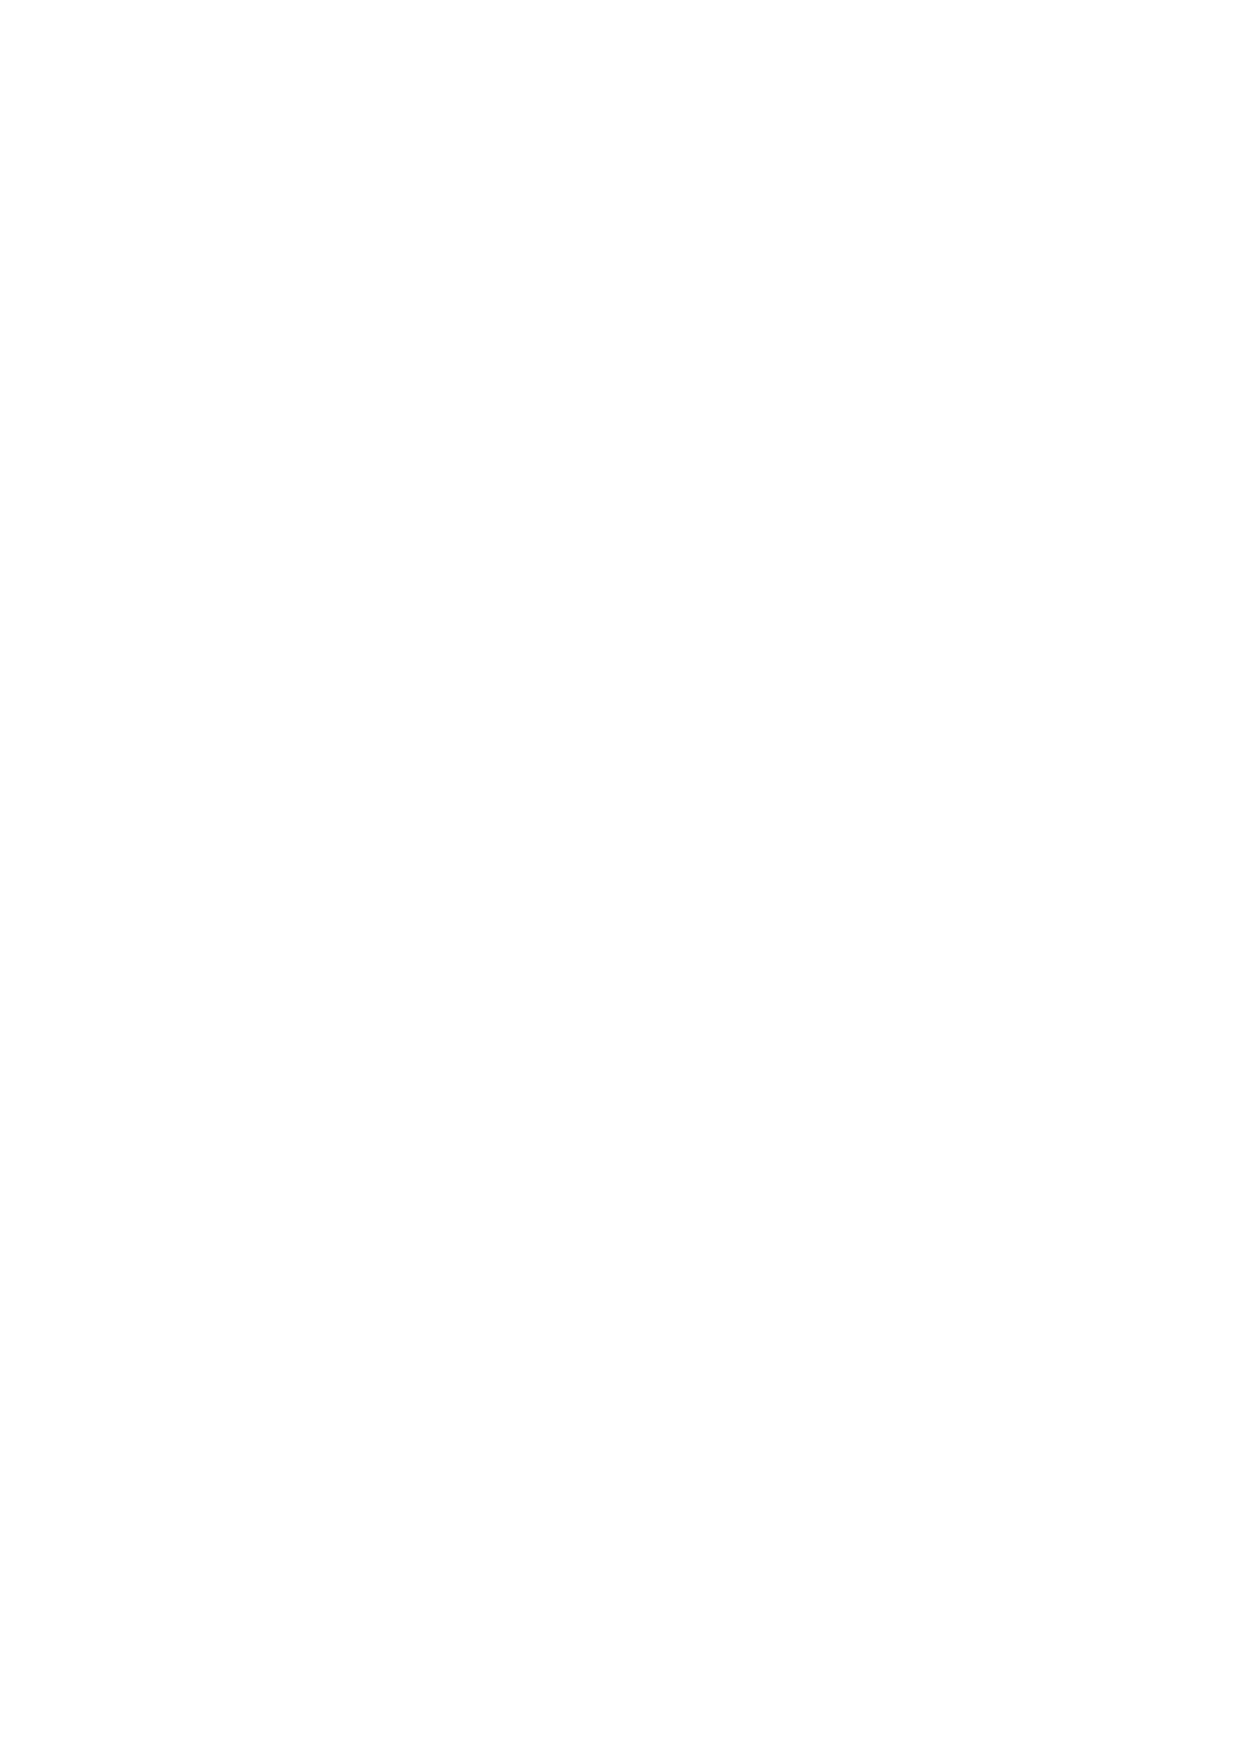
\includegraphics[width=0.8\textwidth]{chap_6_fig_2.pdf}
	\caption{ \textbf{Topological defects in active nematic surfaces.} (i) The charge of the topological defects is related to the number of axes of symmetry (red lines). (ii) Nature of active forces in a self-propelling $\textup{+} 1/2$ defect. Activity can induce a $\textup{+}1$ bound defect. Depending on the sign of activity, a vortex-type  or an aster-type bound defect is formed .}
	\label{fig_0_2}
\end{figure}
\begin{center}
	\begin{mybox}{gray}{\center{\textbf{Box B: Topological defects in active nematics}}}
		Topological defects  are (nearly) singular points with an abrupt gradient in the orientation field. Topological defects on a surface are classified based on their charge $k$ defined using the number of axes of symmetry $n$ as $k = 1 - \vert n/2\vert$ \cite{tang2017}.
		For example, as shown in Fig.~\ref{fig_0_2}, topological defects with $n=3$ and $n=1$ have a defect charge  of $k= \textup{+} 1/2$ and $k=\textup{-} 1/2$ respectively. In a passive nematic system, $\pm 1/2$ defects are stable. Activity renders a $\textup{+}1/2$ motile along its axis of symmetry, whereas due to its three-fold symmetry, a $\textup{-}1/2$ defect does not propel. Contractile (extensile) activity drives a $\textup{+}1/2$ defect in the direction of its tail (comet-head) \cite{thijssen2020,vafa2020}. As a result of activity-driven propulsion, two $\textup{+}1/2$ can overcome their repulsive force to create a bound $\textup{+}1$. For a contractile (an extensile) system, one then gets a $\textup{+}1$ defect with vortex-like (aster-like) structure \cite{thijssen2020, vafa2020}, see Fig.~\ref{fig_0_2}.
	\end{mybox}
\end{center}

For example, at the sub-cellular level, cytokinesis in the final stage of the cell cycle is triggered by the self-organization of a nematic bundle with a high density of actin filaments and bundling proteins in the equator, Fig.~\ref{fig_0}(i) \cite{anne2016, wollrab2016, leite2019}. As a result of this network organization, contractile forces are generated efficiently \cite{kelkar2020} leading to axial elongation  and furrowing in the cytoskeleton dividing a cell in two. A similar mechanism involving the self-organization of contractile rings has been shown to drive cellular deformations in notochord cells, Fig.~\ref{fig_0}(ii) \cite{Dong}, or wound closure after cell ablation, Fig.~\ref{fig_0}(iii) \cite{mandato2001}. %In contrast with the drastic shape changes driven by nematic contractile bundles, recent studies also indicate splitting of nematic tactoid (shown in Fig.~\ref{fig_0}(iv)) via a polarity sorting mechanism involving myosin-II gathering at the tactoids equator and sorting filaments into an aster that pinches the droplet \cite{weirich2017, brugues2014, kaznacheev2002}. 
Defect-modulated shape changes are observed in active nematic vesicles, Fig.~\ref{fig_0}(iv-v), where the motion of defects lead to filopodia-like protrusions. In smaller vesicles, a similar motion of defects leads to a spindle-like structure with two $+1$ defects at the ends of the spindle \cite{keber2014}. 


\begin{figure}[h!]
	\centering
	\includegraphics[width=1\textwidth]{chap_6_fig_1.pdf}
	\caption{ \textbf{Interplay between shape and nematic order at sub-cellular and supra-cellular scales.} (i) Cell division is achieved through the ingression of a dense bundle of contractile actomyosin 
		ring (white arrows) \cite{anne2016}. (ii) Contractile actomyosin ring (yellow arrows) drives constriction and elongation in Notochord cells \cite{Dong}. (iii) Cell wound healing driven by the constriction of a self-organized dense bundle of actomyosin ring around the ablated region \cite{mandato2001}. (iv) Transient shapes characterized by the formation of spikes around $\textup{+}1/2$ (top) and $\textup{+}1$ (bottom) defect sites in a layer of microtubules and kinesin motors in a lipid vesicle \cite{keber2014}. (v)  Morphologies of vesicles formed from nematic amphiphilic block copolymers  as a result of the interplay between nematic ordering and vesicle shape \cite{xing2012}. (vi) Hydra morphogenesis with defects acting as organizational centers. $\textup{+}1$ defect in the proximity of the mouth, the foot and the tip of each tentacle, and two $\textup{-}1/2$ defects at the base of each tentacle \cite{maroudas2021}. (vii) Mounds of myoblast cells protruding out of a $\textup{+}1$ nematic defect \cite{guillamat2020}.}
	\label{fig_0}
\end{figure}


In developing Hydra, an interplay between the nematic alignment of actin, biochemical signaling processes and topological constraints drives morphogenesis, Fig.~\ref{fig_0}(vi) \cite{maroudas2021}. In particular, $+1$ topological defects in Hydra tissue spheroids act as precursors to the development of head/foot, whereas ${\text +}1/2$ defects appear at the base of an early bud, with a $+1$ defect at its tip, as the bud protrudes to form a tentacle. At the supra-cellular level, defect-mediated morphogenesis has been observed in myoblasts cultures  that form cylindrical  multi-cellular  protrusions around spiral- and aster-type topological defects, Fig.~\ref{fig_0}(vii) \cite{guillamat2020}.



The non-trivial relationship between the out-of-equilibrium flows, nemato-dynamics, curvature and topological constraints has been widely explored theoretically and computationally on nearly rigid surfaces, a situation that can be justified by high surface tension or by the presence of  a confining rigid bulk medium  \cite{ellis2018}. These studies have been performed on surfaces such as cylinders \cite{napoli2020, pearce2020}, spheres and prolate/oblate spheroids \cite{nestler2018, torres2020, henkes2017, zhang2020, keber2014, vcopar2019,alaimo2017, ehrig2017,khoromskaia2017,kralj2011}, tori \cite{torres2020, ellis2018}, and nonic surfaces \cite{nestler2018}. These studies show that a genus-zero surface self-organizes defects with a total topological charge of $+2$, following the Poincare-Brouwer theorem \cite{kamien2002}. In the absence of activity, these defects achieve steady low-energy configurations. In a sphere, such configuration is characterized by a  tetrahedral arrangement of defect with an average inter-defect angle of $109.5^{\circ}$, whereas on an ellipsoid defects arrange at the poles \cite{nitschke2020}. The energetic cost of a defect on the surface depends on the local Gaussian curvature \cite{nestler2018, ellis2018}. When activity goes above a critical threshold, these defects become mobile and undergo oscillations between low and high energy configurations. At larger activities, the topological defects enter a regime of irregular and chaotic motion, often accompanied by spontaneous proliferation and annihilation of defects, a regime  called active turbulence \cite{ellis2018,vcopar2019,gao2017}. 

The theoretical models used to study these dynamics can be broadly classified in two approaches: 1) The first approach is based on particle simulations \cite{alaimo2017, ehrig2017,keber2014,khoromskaia2017,ellis2018}, which involves sets of  ordinary differential equations  governing particle positions and orientations. %(ODEs). The first ODE governs the position of the particles accounting for spontaneous directed propulsion due to activity along with repulsive and attractive forces between the particles depending on their topological charge. The second ODE governs the orientation of the active particle accounting for the torque acting on it due to the tendency of particles to align with the neighbours as well as with the direction of its velocity. The coupled ODEs are integrated numerically using standard Euler or Runge-Kutta methods. 
2) In the second approach involves a mean-field continuum description of the dynamics of orientational order and and flow in terms of partial differential equations on a curved surface \cite{vcopar2019,torres2020,zhang2020, napoli2020,pearce2020,nestler2018}. In this approach, the governing equations are solved using the Lattice-Boltzman algorithm \cite{denniston2004} or space discretization schemes based on the finite element method \cite{nestler2018}. 

Shape changes resulting from the interwoven coupling between nematic order, geometric parameters, topological constraints and active hydrodynamics have been explored in fewer studies  \cite{al2021}. \citet{nitschke2020} proposed a thermodynamically consistent mathematical model for the relaxation dynamics of a passive nematic system on a deformable surface. In this model, the free-energy consists of the Helfrich energy, the Landau-de Gennes energy and a surface-area penalization energy.  The numerical formulation is an extension of \cite{nitschke2019}, which was used to study shape evolving surfaces with polar order. They show an interesting interplay between defect configurations and intrinsic/extrinsic curvature contributions. \citet{xing2012} also studied the relationship between the morphology of a passive vesicle and surface nematic order. The study involves a minimalistic mathematical model with the Helfrich energy and a potential similar to the Landau-de Gennes energy that only penalizes the gradients in the orientation field. It is shown that in the limit where the contribution of the Landau-de Gennes energy is far greater than the Helfrich energy, the ground state of a vesicle with spherical topology is a faceted tetrahedron, with $+1/2$ defects located at each of the four corners. On the other hand, in the limit where the relative contribution of Helfrich energy is higher, the ground state is an infinitesimally deformed spherical vesicle with a tetrahedral defect configuration. None of the above-mentioned studies account for the dissipation involved in surface flows nor for activity. 

Recently,  \citet{vafa2021} have proposed a minimal framework for active surfaces coupling frictional flows, nematic order, shape and density. However, other possibly relevant ingredients such as shear dissipation, the dissipative coupling between flow and nematic order and Helfrich energy are not accounted for. Consistent with experimental findings \cite{kawaguchi2017,maroudas2021}, the numerical solution of the model demonstrates that (i)  cell density increases (decreases) at plus (minus) defects, (ii) curvature  is positive (negative) near a plus (minus) defect and (iii) activity can stabilize a ring configuration of equally spaced $\textup{+}1$ defects separated by pairs of $\textup{-}1/2$ defects. \citet{metselaar2019} and \citet{https://doi.org/10.48550/arxiv.2205.06805} have employed more comprehensive active nematic surface models to simulate defect-mediated morphogenesis. The model accounts for orientational order, shape dynamics, surface Stokes flow as well as active tensions. Hybrid lattice-Boltzmann numerical simulations are used to explore the mechanism behind shape changes directed by self-organized topological defects and active flows. \citet{Ruske2021} proposed a theoretical and computational framework to study a related problem in interfacial active nematics, the reshaping of active droplets in 3D, which exhibit in-plane and out-of-plane nematic order at the interface. The proposed governing equations are solved using a hybrid lattice-Boltzmann finite-difference method. %The numerical experiments  show that active stresses cause in-plane (in extensile droplet) and out-of-plane (in contractile droplet)  alignment of the director field at the interface of droplets. This `active anchoring' results from an interplay between active flows and a change in nematic orientation. Such gradient in nematic direction trigger the formation of fingerlike protrusions (in extensile droplets) and surface wrinkles and droplet invagination (in contractile droplets). 

Despite recent efforts, there are two obstacles to study the multiphysics and geometry-dependent mechanics of active and deformable fluid nematic surfaces. The first obstacle involves the need for a general theoretical framework for such a complex system. In the existing literature,  theories for active surfaces have been proposed, which can potentially address this challenge. These frameworks involve two major approaches: (i) The first approach \cite{salbreux2022} is a generic framework for active surfaces and involves identifying the forces and moments acting on a surface to formulate the  governing equations encoding balance of momentum and generalized forces. The calculation of rate-of-change of free-energy identifies the conjugate pairs of thermodynamic forces and fluxes. Lastly, the relationship between conjugate pairs is postulated in terms of linear constitutive laws that satisfy the Onsager relations. (ii) The second approach \cite{torres2019, arroyo2018} is based on Onsager's variational formalism, where the constitutive relationships are implicit in the form of free-energy, dissipative potentials and activity functionals. The governing equations follow from a minimization principle where free-energy release rate, dissipation and activity compete. 

The second obstacle involves the lack of an efficient computation framework to solve resulting Euler-Lagrange equations. The literature on numerical methods for such tensor-valued problems is rare and mainly restricted to the sphere. Here a major difficulty is the approximation of tensor fields such as the nematic field $\bm{q}$ on general surfaces. To address this, \citet{torres2020} proposed a Local Monge parametrization to interpolate  higher-order tensors on arbitrary surfaces. Alternatively, it is possible to interpolate bulk tensors and impose with a penalty the constraint that they should be tangential to the surface \cite{nestler2018,metselaar2019,https://doi.org/10.48550/arxiv.2205.06805}, at the expense of additional degrees of freedom and a stiff term in the equations. 


In the next chapters, we fill this gap by proposing a theoretical framework based on Onsager's variational formalism for active nematic deformable fluid surfaces. This variational method naturally lends itself to finite element discretizations to numerically discretize  the governing equations in space. Furthermore, Onsager's formalism admits a time-incremental variational principle that serves as a time-discretization method and inherits the built-it thermodynamic consistency and nonlinear stability of the time-continuous version. This means that in the absence of power input, the free-energy is a Lyapunov functional of the dynamics. In Chapter~\ref{chap_7}, we formulate the mathematical model, derive the strong form of the coupled equations governing shape dynamics and nemato-hydrodyamics, and interpret these equations. In Chapter~\ref{chap_8}, we focus on the application of the general model to the actin cytoskeleton, and more specifically, to the assembly of the cytokinetic ring leading to cell division. In this model, the surface is compressible and density effects are crucial. We restrict the model to axisymmetry and develop an efficient finite element numerical approach. In Chapter~\ref{chap_9}, we focus on inextensible active liquid crystal nematic vesicles in a fully 3D setting, and propose a general finite element method for active nematic and deformable fluid surfaces. 



\renewcommand{\thesection}{6.\arabic{section}}
\chapter{Theoretical description of an active nematic surface} \label{chap_7}
In this chapter, we propose a generic theory for active nematic deformable surfaces. The state of the system is given by the shape of the surface, the nematic tensor on the surface, and the surface density of cytoskeletal materials, which evolves as a result of local area changes and of turnover. Accounting for density allows us to describe interfacial active gels such as the actomyosin cytoskeleton, which experiences very large density variations often coupled to changes of nematic order. This framework can be very easily adapted to more conventional liquid crystal surface models, where density does not play such an important role, and instead the surface is often considered to be locally inextensible. Such a model is developed in Chapter~\ref{chap_9} and is pertinent for instance to active nematic gels deforming on lipid vesicles. Our derivation is based on the variational framework for active surfaces proposed in \cite{torres2019}. We start by describing the state variables of the model, followed by the process variables describing their evolution. We then resort to Onsager's variational formalism to systematically derive the Euler-Lagrange equations of the model. As described in previous chapters, the variational formulation is useful for coupling surface flow with other relevant mechanical and chemical effects as well as for numerical finite element implementations. At the core of the variational framework is the Lagrangian of the system formulated as the sum of  1) a dissipation potential encoding the passive and unrecoverable energetic cost of changing the state of the system, 2) the rate-of-change of the free-energy potential describing the release rate or reversible work, 3) a power potential capturing the active power input and 4) the work performed by Lagrange multipliers to subject the system to mechanical constraints. The Lagrangian functional is minimized with respect to the process variables and maximized with respect to the Lagrange multipliers to derive the  Euler-Lagrange equations in a thermodynamically consistent manner. In this model, in the absence of active power input, the free-energy is by construction a Lyapunov function of the dissipative dynamics.  For an extensible surface, the model is complemented by a mass balance equation describing turnover.  

The outline of this chapter is as follows. In Section~\ref{sec4_2_1}, we start by introducing our notations and the differential geometry required to describe the state and process variables of a nematic surface. In Section~\ref{sec4_2_2}, we derive the  strong form of a thermodynamically consistent nematic active deformable surface following Onsager's variational formalism. Finally, in Section~\ref{sec4_2_4}, we summarize our results.

\section{Kinematics of nematic surfaces} \label{sec4_2_1} 

\subsection{Differential geometry and covariant derivatives}

We describe the dynamics of a two-dimensional continuum $A$ in $\mathbb{R}^3$ using a time-dependent parametrization of the surface $\bm{x}=\bm{\phi}(\bm{\xi},t)$ from a reference domain $\bar{A}$ with coordinates $\bm{\xi}=\{\xi^1, \xi^2$\}  in $\mathbb{R}^2$, see Fig.~\ref{fig_7.1}. This time-dependent map can be interpreted as a Lagrangian parametrization, i.e.~for a fixed $\bm{\xi}$, $\bm{\phi}(\bm{\xi},t)$ tracks the trajectory of a material particle. At any instant $t$ and coordinate $\bm{\xi}$, the natural or convected basis vectors of the tangent plane to $A$ are given by $\bm{e}_1 = \partial_{1} \bm{\phi}$ and $\bm{e}_2 = \partial_{2} \bm{\phi}$, where $\partial_a = \partial / \partial \xi^a$. In general, these basis vectors are neither of unit length nor orthogonal. The  normal vector to $A$ at $\bm{x}=\bm{\phi}(\bm{\xi})$ is given by $\bm{N} = (\bm{e}_1 \times \bm{e}_2)/\left|\bm{e}_1 \times \bm{e}_2 \right|$. Here and in the following, we use upper-case letters to denote three-dimensional tensors and lower-case letters for tensors tangent to $A$, i.e.~without a normal component. 
\begin{figure}[h!]
	\centering
	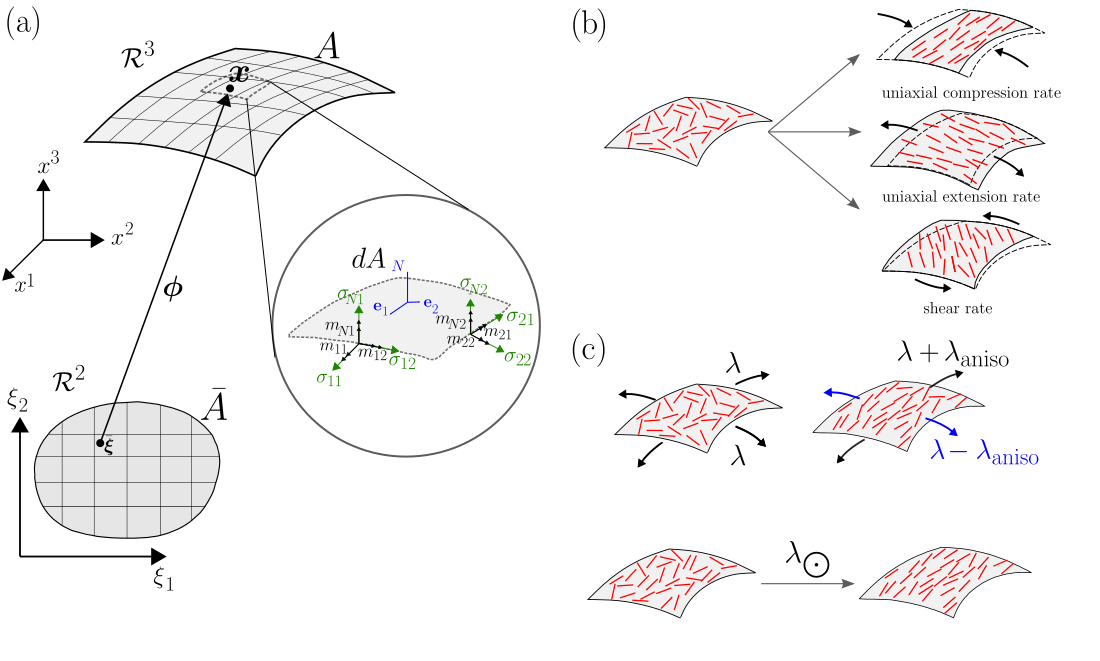
\includegraphics[width=1\textwidth]{chap_7_fig_1.pdf}
	\caption{(a) Illustration of the surface parametrization, with the induced local basis of the tangent space given by  $\bm{e}_1$ and $\bm{e}_2$, and the normal unit vector $\bm{N}$. The inset shows the different stress components, including the in-plane stress $\bm{\sigma}$, the out-of-plane stress $\bm{\sigma}_N$, the in-plane moment $\bm{m}$ and the out-of-plane moment $\bm{m}_N$. (b) A compression (extension) in the local area results in an emergent nematic order with molecular aligned on average perpendicular (along) to the principal direction of the rate of deformation tensor $\bm{d}$. A shear in the local area  due to traceless $\bm{d}^{\rm dev}$ tends to align fibers clockwise or counter-clockwise depending on the direction in which the differential area element distorts. (c) $\lambda \bm{g}$ characterizes the base value of the emergent isotropic active stress per unit volume resulting from the action of actin bundling proteins in an isotropic network.  $\lambda_{\rm aniso} \bm{q}$ characterizes the base value of emergent  anisotropic active stress per unit volume resulting from the action of actin bundling proteins in an anisotropic network along ($\lambda_{\rm aniso}>0$) or perpendicular ($\lambda_{\rm aniso}<0$) the average molecular orientation $\bm{n}$.  $\lambda_{\bigodot}\bm{q}$ characterizes the basal active torque per unit volume exerted by the actin bundling proteins resulting in filament rotational movement.}
	\label{fig_7.1}
\end{figure} 
We define the dual basis $\{\bm{e}^1,\bm{e}^2\}$, satisfying the conditions
\begin{equation} \label{2_II}
	\bm{e}^a \cdot \bm{e}_b = \delta^a_b,
\end{equation}
where here $\cdot$ stands for the scalar product in Euclidean space. 
Given a tangent vector $\bm{v}$, we can represent it in terms of the natural and dual basis, $\bm{v}=v^a\bm{e}_a=v_a\bm{e}^a$. We call $v^a$ the contravariant components of $\bm{v}$ and $v_a$ the covariant components of $\bm{v}$. Given that $\bm{v}$ is also embedded in Euclidean space, we can represent it as $\bm{v}=v^\alpha \bm{E}_\alpha$ where the vectors $\bm{E}_\alpha$, $\alpha=1,2,3$ form an orthonormal basis of Euclidean space. In the following, we use Latin indices, running from $1$ to $2$, for components in the tangent plane and Greek indices, running from $1$ to $3$, for components in Euclidean space. 

The metric tensor $\bm{g}$ can be used to compute the scalar product of vectors on $A$: given two tangent vectors $\bm{v} = v^a \bm{e}_a$ and  $\bm{w} = w^b \bm{e}_b$, their scalar product is $\bm{v}\cdot\bm{w}=\bm{g}(\bm{v},\bm{w})=g_{ab} v^a w^a$. Since $\bm{v}\cdot\bm{w}$ is also defined in Euclidean space, this equivalence can be used to find the components of $\bm{g}$ in the basis $\{\bm{e}^1,\bm{e}^2\}$:
\begin{equation} \label{eq::metric}
	g_{ab} = \bm{e}_a \cdot \bm{e}_b.
\end{equation}
The inverse of $\bm{g}$, $\bm{g}^{-1}=g^{ab}\bm{e}_a\otimes\bm{e}_b$, satisfies $g^{ac}g_{cb} = \delta^a_{~b}$. We note that $\bm{e}^a$ and $\bm{e}_a$ satisfy
\begin{equation} \label{2_II}
	\bm{e}^a = g^{ab}\bm{e}_b,\qquad \bm{e}_a = g_{ab}\bm{e}^b.
\end{equation}
Similarly, the contravariant and covariant components of a vector satisfy 
\begin{equation}
	v_a = g_{ab} v^b,\qquad v^a = g^{ab} v_b. 
\end{equation}
These operations are referred to as lowering and raising an index.

The curvature tensor on $A$, $\bm{k}$, measuring how much the surface deviates from a plane, can be defined through derivatives of $\bm{N}$. In particular $k_{ab}$ measures the rate of change of $\bm{N}$ along $\bm{e}_a$ in the direction of $\bm{e}_b$,
\begin{equation} \label{3_II}
	k_{ab} = \partial_b \bm{N} \cdot \bm{e}_a = -\bm{N} \cdot  \partial_a  \partial_b \bm{\phi},
\end{equation}
where to get to the last expression we have used the product rule and that $\bm{N} \cdot \bm{e}_a=0$.
The antisymmetric tensor $\bm{\epsilon}$, satisfying $\epsilon_{ab}=-\epsilon_{ba}$ and $\epsilon_a{}^c \epsilon^b{}_c=\delta_a^b$ has components
\begin{equation} \label{4_II}
	\epsilon_{ab} = \bm{N} \cdot (\bm{e}_a \times \bm{e}_b).
\end{equation}

To measure derivatives of tensors on $A$, we use the covariant derivative $\nabla$, which accounts for the fact that both the components of a tensor and the basis vectors vary along the curvilinear coordinates. For a vector, $\nabla\bm{v}$ has components
\begin{equation} \label{6_II}
	\nabla_b v^a = \partial_b v^a + \Gamma^a{}_{bc} v^c.
\end{equation}
where $\Gamma^c_{~ ab}$ are the Christoffel symbols of the basis $\{\bm{e}_1,\bm{e}_2\}$. These quantities  measure the rate of change of $\bm{e}_a$ along $\bm{e}_b$ in the direction of $\bm{e}^c$,
\begin{equation} \label{8_II}
	\Gamma^c_{~ ab} = \bm{e}^c\cdot \partial_b \bm{e}_a=\bm{e}^c\cdot \partial_b \partial_a \bm{\phi},
\end{equation}
and can be expressed intrinsically in terms of derivatives of the metric tensor alone \cite{Do_Carmo2016-kq}.
Given that $\partial_b \partial_a \bm{\phi}=\partial_a \partial_b \bm{\phi}$, we have $\Gamma^c_{~ ab}= \Gamma^c_{~ba}$. The covariant derivative
$\nabla\bm{v}$ can be defined intrinsically to the surface $A$ seen as a Riemannian manifold without reference to the embedding Euclidean space. It can also be related to the  usual gradient in $\mathbb{R}^3$ by
\begin{equation}\label{cov_der}
	\nabla \bm{v} = \mathbb{P}\,\nabla^{\rm 3D} \bm{v}\,\mathbb{P}
\end{equation}
where $\mathbb{P}=\bm{e}^a\otimes\bm{e}_a$ is the projector operator on the surface and $\otimes$ is the tensor product (see Appendix~\ref{velocity_gradient}). The projector on the right restricts the derivative to the plane, whereas the projector on the left ensures that the result is tangent to $A$. Computing $\nabla^{\rm 3D}$ requires extending the field $\bm{v}$ outside of $A$, but it can be shown that the result is independent of the extension because of the action of the right projector. 
The covariant derivative of $\bm{v}$ written in terms of its covariant components is given by
\begin{equation} \label{6_II_b}
	\nabla_b v_a = \partial_b v_a - \Gamma^c_{ab} v_c.
\end{equation}
For a generic tensor $\bm{T}$ described with $m$ contravariant and $n$ covariant components, the definition of the covariant derivative is
\begin{align} \label{7_II}
	\nabla_c T^{a_1\dots a_m}_{~ \, \, \, \, \, \, \, \, \, \, \, \, \, \, \, \,   b_1 \dots b_n} =  {}&  \partial_c T^{a_1 \dots a_m}_{~ \, \, \, \, \, \, \, \, \, \, \, \, \, \, \, \, b_1 \dots b_n}  + \Gamma^{a_1}_{cd} T^{d\dots a_m}_{~ \, \, \, \, \, \, \, \, \, \, \, \, \, \, \, \,   b_1 \dots b_n} + \Gamma^{a_2}_{cd} T^{a_1 d\dots a_m}_{~ \, \, \, \, \, \, \, \, \, \, \, \, \, \, \, \,   b_1 \dots b_n} + \left(\text{all upper indices}\right)   \nonumber\\ & - \Gamma^d_{c b_1} T^{a_1 \dots a_m}_{~ \, \, \, \, \, \, \, \, \, \, \, \, \, \, \, \, d \dots b_n} -  \Gamma^d_{c b_2} T^{a_1 \dots a_m}_{~ \, \, \, \, \, \, \, \, \, \, \, \, \, \, \, \, b_1 d \dots b_n}  - \left(\text{all lower indices}\right),
\end{align}
Notably, 
\begin{align} \label{10_II}
	\nabla\bm{g} = \nabla\bm{g}^{-1} = \nabla\bm{\epsilon} = \bm{0},
\end{align}
We can extend the notion of the covariant derivative to 3D tensors defined over $A$. For instance, given a vector $\bm{V}$,
\begin{equation}\label{cov_derV}
	\nabla \bm{V} = \nabla^{\rm 3D} \bm{V}\,\mathbb{P},
\end{equation}
Note that here, the right projector is used again to restrict the computation to variations along the tangent plane, whereas the left projector is absent given that we want to know how the vector is changing in Euclidean space. This is a $3\times2$ tensor with first component in Euclidean space and second component tangent to $A$. Eq.~\eqref{cov_derV} can be rewritten in terms of the in-plane  and normal components of $\bm{V} = \bm{v} + v_N \bm{N}$ as
\begin{equation}
	\label{eq::velgrad}
	\nabla \bm{V}= \left(\nabla_b v^a+v_n k_b{}^a \right) \bm{e}_a \otimes \bm{e}^b + \left(\nabla_a v_n - k_{ab} v^b \right) \bm{N} \otimes \bm{e}^a.
\end{equation}
See Appendix~\ref{velocity_gradient} for a derivation. 

\subsection{Velocity, rate of deformation, and spin}

The velocity field is defined as
\begin{equation} \label{14_II}
	\bm{V} = \partial_t \bm{\phi}(\bm{\xi},t) = \bm{v} + v_N \bm{N},
\end{equation}
where the normal velocity $v_N$ characterizes the rate of change of the shape of $A$ and $\bm{v}$ describes the in-plane flow. The velocity gradient is given by the covariant derivative of $\bm{V}$ defined by Eq.~\eqref{eq::velgrad}. On a plane, we have seen previously in this thesis that we can split the velocity gradient into its symmetric and antisymmetric parts
\begin{equation}\label{qwe}
	\nabla\bm{v} = \bm{d} + \bm{w}
\end{equation}
where $\bm{d}$ ($=\bm{d}^T$), the rate-of-deformation tensor, characterizes the strain rate and $\bm{w}$ ($=-\bm{w}^T$) the spin tensor, characterizes the local rotation generated by the flow. We seek a similar decomposition for $\nabla\bm{V}$. We first note that the rate-of-deformation tensor admits the following geometric definition \cite{marsden1994}
\begin{equation}\label{eq6:lie-der}
	\bm{d}=\frac{1}{2}\mathcal{L}_{\bm{V}}\bm{g},
\end{equation}
where $\mathcal{L}_{\bm{V}}\bm{g}$ is the Lie derivative of $\bm{g}$. This quantity measures the rate of change of the metric tensor $\bm{g}$ as seen by an observer that deforms with the flow generated by $\bm{V}$. The Lie derivative satisfies the product rule, which allows us to compute the Lie derivative of the inverse of the metric. Because $0 = \mathcal{L}_{\bm{V}} \delta^a_b = \mathcal{L}_{\bm{V}}(g^{ac}g_{cb}) = g_{cb}\mathcal{L}_{\bm{V}}g^{ac} + g^{ac}\mathcal{L}_{\bm{V}}g_{cb} = g_{cb}\mathcal{L}_{\bm{V}}g^{ac} + 2 g^{ac}d_{cb}$, we conclude that $\mathcal{L}_{\bm{V}}g^{ab} = -2 d^{ab}$, or tensorially 
\begin{equation}\label{eq6:lie-der_}
	\bm{d}= - \frac{1}{2}\mathcal{L}_{\bm{V}}\bm{g}^{-1}.
\end{equation}

Because our parametrization is Lagrangian, its components are given in the natural convected basis of the surface by $\mathcal{L}_{\bm{V}}g_{ab} = \partial_t\left(\bm{e}_a\cdot\bm{e}_b\right)=\bm{e}_a\cdot\partial_b\bm{V} + \bm{e}_b\cdot\partial_a\bm{V}$, which can be written in terms of $\nabla\bm{V}$ as
\begin{equation}
	\label{eq6:d}
	\bm{d} = {\rm sym}\left(\mathbb{P}\,\nabla \bm{V}\right)= \frac{1}{2}\left[\nabla \bm{v} + \left(\nabla\bm{v}\right)^T\right] + v_N \bm{k}.
\end{equation}
Since $\bm{g}$ determines the length and angle between vectors on $A$, $\mathcal{L}_{\bm{V}}\bm{g}$ characterizes the rate at which objects deform on the surface \cite{torres2017}. For instance, the trace of $\bm{d}$ characterizes the rate of change of an infinitesimal area
\begin{equation}\label{eq6:dSdt}
	\frac{1}{dS}\dfrac{d}{dt}dS = \textup{tr}\bm{d} = d_{ab}g^{ab} = \nabla \cdot \bm{v} + v_N H,
\end{equation}
where $\nabla \cdot \bm{v}=\nabla_a v^a$ is the divergence of the in-plane velocity and $H=\textup{tr}(\bm{k})$ is the total curvature (twice the mean curvature).

To find an expression analogous  to Eq.~(\ref{qwe}) in the surface setting, we examine the structure of $\nabla \bm{V} - \bm{d}$, which should yield the generalization of the spin tensor. Combining Eqs.~(\ref{eq::velgrad}) and (\ref{eq6:d}), it follows that this difference can be uniquely expressed in terms of a three-dimensional spin tensor $\bm{W}$, satisfying $\bm{W}^T=-\bm{W}$, as
\begin{equation}
	\nabla \bm{V} - \bm{d} = \bm{W} \mathbb{P},
\end{equation}
where
\begin{equation}
	\bm{W} = \frac{1}{2}\left(\nabla_b v_a - \nabla_a v_b\right) \bm{e}^a\otimes \bm{e}^b + \left(\nabla_a v_N - k_{ab} v^b \right) \left(\bm{N} \otimes \bm{e}^a -  \bm{e}^a\otimes \bm{N}\right).
\end{equation}
The first component arises from local in-plane rotations rates and corresponds to the previously considered spin tensor in the flat case. The second component represents the local rotation rate of the surface tangent plane in $\mathbb{R}^3$. Thus, the velocity gradient can be decomposed into the rate of deformation tensor and the projection onto the tangent plane to $A$ of a three-dimensional spin tensor
\begin{equation}
	\nabla \bm{V} = \bm{d} + \bm{W} \mathbb{P}.
\end{equation}
One can also define the spin vector, $\bm{\Omega} = \bm{W}^\star$, the Hodge-dual of $\bm{W}$ in $\mathbb{R}^3$, whose Cartesian components are
\begin{equation} \label{omega_alpha}
	\Omega^\alpha = \mathcal{E}^{\alpha\beta\gamma} W_{\beta\gamma} = \omega_a  e^{a\alpha} + \omega_N N^{\alpha}.
\end{equation}
where $\bm{\mathcal{E}}$ is the 3D Levi-Civita tensor and where
\begin{align}
	\bm{\omega} &= \bm{\epsilon}\left(\nabla v_N - \bm{k}\bm{v}\right),\label{eq6:omega}\\
	\omega_N &= \frac{1}{2} \epsilon^{ab} \nabla_b v_a. \label{eq6:omegaN}
\end{align}
In Eq.~(\ref{omega_alpha}), $e^{a\alpha}$ denotes the $\alpha$-th Cartesian component of tangent vector $\bm{e}^a$. The spin tensor can be recovered from the spin vector from $W^{\alpha\beta} = \mathcal{E}^{\alpha\beta\gamma}\Omega^\gamma$. 

The covariant derivative of the spin vector, quantifying the gradients of rotation rate, is given by
\begin{equation}
	\bm{\mathcal{Z}} =\nabla \bm{\Omega}  = \zeta^a{}_b\bm{e}_a \otimes \bm{e}^b + \zeta_{na} \bm{N} \otimes \bm{e}^a,
\end{equation}
where
\begin{align}
	\bm{\zeta} &= \nabla \bm{\omega}+\omega_N\bm{k},\label{eq6:xi}\\
	\bm{\zeta}_N &= \nabla \omega_N-\bm{k}\bm{\omega}\label{eq6:xiN}.
\end{align}
The Lie derivative of the curvature tensor (with covariant indices) can be written in terms of $\bm{\zeta}$ and $\bm{d}$ as
\begin{align} \label{26_II}
	\mathcal{L}_{\bm{V}} \bm{k}  = & -\frac{1}{2} \left(\bm{\zeta} +\bm{\zeta}^T\right)+ \frac{1}{2}\left(\bm{k}\,\bm{d} +\bm{d}\,\bm{k}\right),
\end{align}
see Appendix~\ref{curvature_tensor}.
Similarly, the rate of change of the Christoffel symbols in the convected basis satisfies
\begin{equation}\label{25_II}
	 \zeta_{Nc} = \frac{1}{2}\partial_t\Gamma^a_{bc} \epsilon_a^{~b} .
\end{equation}
%see Appendix~\ref{christoff_symbols}.

\subsection{Nematic order}


Another state variable characterizing the system is the nematic order tensor $\bm{q}$, which measures orientational order tangentilly to $A$. Mathematically, it is expressed as
\begin{equation} \label{27_II}
	\bm{q} = S\left(\bm{n}\otimes\bm{n} - \frac{1}{2}\bm{g}\right),
\end{equation}
where $\bm{n}$, a vector, represents the local director field and $S=\sqrt{2q_{ab}q^{ab}}$, the nematic order parameter, represents the strength of alignment about $\bm{n}$. The nematic tensor is both symmetric, $\bm{q} = \bm{q}^T$, and traceless $\textup{tr}\bm{q}=0$. We now need to define an objective rate for $\bm{q}$. In 2D, we have used the Jaumann derivative,
\begin{equation}\label{eq6:Lie-der-q}
	\widehat{\bm{q}} = \partial_t\bm{q} + \bm{v}\cdot\nabla\bm{q} + \bm{q}\bm{w} + \bm{w}\bm{q}.
\end{equation}
We cannot translate this equation directly to the case of a nematic field evolving on a deforming surface since each of the terms do not have a clear translation. To make sense of the Jaumann derivative in our more general situation, we note that objective rates of tensors can be expressed geometrically in terms of Lie derivatives of such tensors \cite{marsden1994}. Indeed, the Jaumann derivative can be expressed as the average of the Lie derivatives of the covariant and of the contravariant forms of the nematic tensor 
\begin{align}\label{jaum_1}
	\widehat{q}^{ab}  = \frac{1}{2}\left(\mathcal{L}_{\bm{V}} q^{ab}  +  g^{ae}g^{bf} \mathcal{L}_{\bm{V}} q_{ef}  \right). 
\end{align}
This definition can be naturally extended to covariant and mixed tensors as
\begin{align}
	\widehat{q}_{ab}  = \frac{1}{2}\left(g_{ae}g_{bf} \mathcal{L}_{\bm{V}} q^{ef}  + \mathcal{L}_{\bm{V}} q_{ab}  \right), 
\end{align}
and 
\begin{align}
	\widehat{q}^a_{~b}  = \frac{1}{2}\left(\mathcal{L}_{\bm{V}} q^{ac} g_{cb}  +  g^{ac} \mathcal{L}_{\bm{V}} q_{cb}  \right).  
\end{align}
Such geometric definitions make perfect sense on a deforming surface, and hence can be used to define the Jaumann derivative of $\bm{q}$ on $A$. These definitions of Jaumann derivative admit physically appealing alternative forms. Raising indices of $q_{ef}$ in Eq.~(\ref{jaum_1}), using the product rule for the Lie derivative, and recalling the geometric definition of the rate-of-deformation tensor, this expression can be recast as
\begin{align}\label{28_II}
	\widehat{q}^{ab}  =\frac{1}{2}\left[\mathcal{L}_{\bm{V}} q^{ab}  +   g^{ae}g^{bf}\mathcal{L}_{\bm{V}} \left(q^{dc}g_{de}g_{cf}\right) \right] = \mathcal{L}_{\bm{V}} q^{ab} + d^a_{~c} q^{cb}   +  q^{ac} d^b_{~c}. 
\end{align}
Analogously, we find  
\begin{align}\label{28_II_}
	\widehat{q}^a_{~b}  = \mathcal{L}_{\bm{V}} q^a_{~b} +  d^a_{~c} q^c_{~b}  -  q^a_{~c} d^c_{~b}, 
\end{align}
and
\begin{align}\label{28_II__}
	\widehat{q}_{ab}  = \mathcal{L}_{\bm{V}} q_{ab} -  d_{ac} q^c_{~b}  -  q_{ac} d^c_{~b}.
\end{align}

Noting that $\mathcal{L}_{\bm{V}} \bm{q}$  can be interpreted as the rate of change of $\bm{q}$ measured by an observer that translates, rotates, and deforms with the flow, Eqs.~(\ref{28_II}-\ref{28_II__}) show that the Jaumann derivative can be interpreted as the rate of change of $\bm{q}$ measured by an observer that translates and rotates, but does not deform with the flow. Intuitively, the last two terms subtract changes in $\mathcal{L}_{\bm{V}} \bm{q}$ induced by strain rate. 

We discuss next some important properties of the Jaumann derivative. As opposed to $\mathcal{L}_{\bm{V}} \bm{q}$, the Jaumann derivative as defined  above is traceless since 
\begin{align}
	{\rm tr}\widehat{\bm{q}}&=g_{ab}\widehat{q}^{ab}= g_{ab}\left(\mathcal{L}_{\bm{V}} q^{ab} + \frac{1}{2}q^{ac}g^{bd}\mathcal{L}_{\bm{V}} g_{cd} + \frac{1}{2}q^{bc} g^{ad} ~\mathcal{L}_{\bm{V}} g_{dc}\right) \nonumber \\ 
	&=g_{ab}\mathcal{L}_{\bm{V}} q^{ab} + q^{ab} \mathcal{L}_{\bm{V}} g_{ab} = \mathcal{L}_{\bm{V}}(q^{ab} g_{ab}) = 0.
\end{align}

It is also important to note a fundamental difference between covariant, Jaumann, and Lie derivatives with regards to raising and lowering indices. Because $\nabla \bm{g} = \bm{0}$, the covariant derivative commutes with the operation of raising or lowering indices. Instead, because $\mathcal{L}_{\bm{V}} \bm{g}  = 2\bm{d}$ and $\mathcal{L}_{\bm{V}} \bm{g}^{-1}  = -2\bm{d}$ are not zero in general, the Lie derivative does not commute with raising and lowering indices. For the Jaumann derivative, a simple calculation shows that Eq.~(\ref{28_II}) applied to $g^{ab}$ leads to $\widehat{g}^{ab} =0$, and analogously Eq.~(\ref{28_II__}) applied to $g_{ab}$ leads to $\widehat{g}_{ab} =0$. Hence, the Jaumann derivative commutes with raising and lowering indices. 


\subsection{Density field}

Finally, we model the density of the network with a scalar field $\rho(\bm{\xi},t)$. Its corresponding process variable is its material time derivative $\dot\rho$. Density obeys the equation of balance of mass, expressed as
\begin{align}  \label{45_II_}
	\dot\rho  + \rho \, \textup{tr }\bm{d} - D \Delta \rho =  s \, ,
\end{align}
where the second term on the left-hand-side is the change of density due to local area changes, the third term models diffusion with $\Delta \rho = g^{ab}\nabla_a\nabla_b \rho$ and the source term $s$ accounts for turnover and often adopts the form  $s = -k_d(\rho-\rho_0)$, with $k_d$ the depolymerization rate and $\rho_0$ the steady-state density. 

For convenience in our derivation, we group the diffusion and the source terms in $r= s+D \Delta \rho$ to write 
\begin{align}  \label{45_II}
	\dot\rho  + \rho \, \textup{tr }\bm{d}  =  r.
\end{align}

\section{Derivation of the governing equations} \label{sec4_2_2}

In this section, we formulate a thermodynamically consistent active nematic model on a deformable surface using Onsager's variational formalism, which provides a transparent and systematic procedure to formulate mathematical models for such complex systems. 

\subsection{Rate of change of free energy}

We consider the Landau-de Gennes-Helfrich energy functional given by
\begin{align} \label{33_II}
	\mathcal{F}[ \bm{q}, \bm{x}, \rho] = {\int_A} f \rho \,d A \, ,
\end{align}
where for convenience we decompose \textit{f} as
\begin{equation}  \label{33_II}
	\mathcal{F}[ \bm{q}, \bm{x}, \rho] = {\int_A} \left(f_{\rm bend} + f_{\rm sus} + f_{\rm frank}\right) \rho \,d A.
\end{equation}
The Helfrich energy is given by  
\begin{equation}  \label{34_II}
	f_{\rm bend}(\bm{x}) = \frac{ \mathcal{B} }{2} H^2,
\end{equation}
where $\mathcal{B}$, the bending rigidity, penalizes the total curvature $H = \textup{tr}\bm{k}$ of the surface. The rest of the free energy terms are based on the Landau-de Gennes functional \cite{de1993} and given by %\marino{[there was a typo]}
\begin{align}   \label{35_II}
	f_{\rm sus}(\bm{q}, \bm{x}) = {a}\, \text{tr}\,\bm{q}^2 + \frac{b}{2}\, \left(\text{tr}\,\bm{q}^2\right)^2,
\end{align}
and
\begin{align} \label{36_II}
	f_{\rm frank}(\bm{q}, \bm{x}) = \frac{L}{2}\nabla_c q_{ab} \nabla^c q^{ab}.
\end{align}
For $a>0$ and $b>0$, the susceptibility energy represents the energy stored as the system deviates away from an entropically favored state of isotropy. When $a<0$, this energy favors spontaneously ordered states. The term with the frank constant $L$ penalizes the nematic deformation modes such as splay and bend. 

The rate of free energy potential can be computed using Reynolds transport theorem, integration by parts and the fact that we consider a surface without boundary  as
\begin{align} \label{37_II}
	\dot{\mathcal{F}}[ \bm{q}, \bm{x}, \rho;  \widehat{\bm{q}}, \bm{v}, v_N]   = & \frac{d}{dt}{\int_A}  f (\bm{q}, \bm{x})  \rho d A   \nonumber \\= &  {\int_A} \bigg [  \dot f \rho +  f \dot\rho +  f \rho  {\rm tr} \bm{d}   \bigg ] d A , 
\end{align}
where we have used Eq.~\eqref{eq6:dSdt}. Note that the arguments of this functional include the parametric dependence of the current state $( \bm{q}, \bm{x}, \rho)$, and the dependence on the process variables controlling the rate of change of the state $( \widehat{\bm{q}}, \bm{v}, v_N)$. Recalling Eq.~(\ref{45_II}), it is clear that the rate of change of density depends on $\bm{v}$ and  $v_N$.

Since $\dot{f}  =  \dot{f}_{\rm bend} +  \dot{f}_{\rm sus} + \dot{f}_{\rm frank}$, we can conveniently write $\dot{\mathcal{F}}$ as
\begin{align}   \label{40_II}
	\dot{\mathcal{F}} = \dot{\mathcal{F}}_{\rm bend} +   \dot{\mathcal{F}}_{\rm sus} +  \dot{\mathcal{F}}_{\rm frank},
\end{align}
where e.g.,
\begin{align}  \label{41_II}
	\dot{\mathcal{F}}_{\rm bend}  = {\int_A} \bigg [  \dot f_{\rm bend} \rho +  f_{\rm bend} \dot\rho +  f_{\rm bend} \rho  {\rm tr} \bm{d}   \bigg ] d A \,  .
\end{align}
% \begin{align}  \label{42_II}
	%  \dot{\mathcal{F}}_{\rm sus}[ \bm{q}, \bm{x}, \rho;  \widehat{\bm{q} }]  =\underset{A}{\int} \bigg [  \dot f_{\rm sus} \rho +  f_{\rm sus} \dot\rho +  f_{\rm sus} \rho  {\rm tr} \bm{d}   \bigg ] d A \,  ,
	% \end{align}
% \begin{align}  \label{43_II}
	%  \dot{\mathcal{F}}_{\rm frank}[\bm{q}, \bm{x}, \rho;  \widehat{\bm{q} },\bm{d}, \bm{w}, \bm{\xi}_{N},w_N]  =\underset{A}{\int} \bigg [  \dot f_{\rm frank} \rho +  f_{\rm frank} \dot\rho +  f_{\rm frank} \rho  {\rm tr} \bm{d}   \bigg ] d A \,  ,
	% \end{align}
Noting that $H=g^{ab}k_{ab}$, that $\dot{a}=\mathcal{L}_{\bm{V}} a$ for a scalar field, and that the Lie derivative satisfies the product rule, i.e.~$\mathcal{L}_{\bm{V}} H = k_{ab}\mathcal{L}_{\bm{V}}g^{ab}+g^{ab}\mathcal{L}_{\bm{V}}k_{ab}$, we get
\begin{equation}  \label{46_II}
	\begin{aligned}
		\dot{\mathcal{F}}_{\rm bend} &= {\int_A}  \left[\mathcal{B}H\left( g^{ab}\mathcal{L}_{\bm{V}}k_{ab} +  k_{ab} \mathcal{L}_{\bm{V}}  g^{ab}\right)\rho  + \frac{1}{2} \mathcal{B}H^2 r  \right]  d A \\
		&= {\int_A}  \left[\mathcal{B}H\left( -g^{ab}\zeta_{ab} -d^{ab} k_{ab}  \right)\rho+\frac{1}{2} \mathcal{B}H^2 r\right]  d A. 
	\end{aligned}
\end{equation}
where we have used Eqs.~\eqref{26_II}, \eqref{45_II} and \eqref{eq6:lie-der_}.

Similarly, for $\dot{\mathcal{F}}_{\rm sus}$ we obtain %\marino{[here, the derivation was a bit off. you cannot put $2q_{~a}^b \mathcal{L}_{\bm{V}} q^{a}_{~b}$ in this equation. also, typo in coefficient with $a$ and $b$]}
\begin{align} \label{48_II}
	\dot{\mathcal{F}}_{\rm sus}  =  {\int_A} & \bigg[(a+bS^2/2)\left(q_{~a}^b \mathcal{L}_{\bm{V}} q^{a}_{~b} + \mathcal{L}_{\bm{V}}q_{~a}^b  q^{a}_{~b} \right) +    \left(\frac{a}{2}S^2 + \frac{b}{8}S^4\right)r \bigg]  \rho d A.
\end{align}
Using Eq.~\eqref{28_II_} to compute the Lie derivatives of the mixed nematic tensors, a simple calculation shows that
\begin{align} \label{49_II}
	\dot{\mathcal{F}}_{\rm sus}  =   {\int_A}& \left[ (2a+bS^2)q_{ab} \widehat{q}^{ab} \rho + \left(\frac{a}{2}S^2 + \frac{b}{8}S^4\right)r  \right]d A.
\end{align}
where we have used that the Jaumann derivative commutes with raising  indices.

For the rate of change of the Frank energy, we have %\marino{[this one I have barely checked]}
\begin{align} 
	\dot{\mathcal{F}}_{\rm frank}  =  {\int_A} \nonumber & L \bigg[\big( \nabla_d  q^b_{~a}\mathcal{L}_{\bm{V}} \nabla_c q^{a}_{~b}g^{dc} \rho  + \frac{1}{2}\nabla_d q^b_{~ a} \nabla_c q^{a}_{~b}\mathcal{L}_{\bm{V}}  g^{dc} \rho + \\ & \frac{1}{2} \nabla_c q^{a}_{~ b}  \nabla^c q^{b}_{~ a} \mathcal{L}_{\bm{V}} \rho  \big) d A    + \frac{1}{2} \nabla_c q^{a}_{~b}  \nabla^c q^{b}_{~ a} \rho \mathcal{L}_{\bm{V}} d A \bigg]. \nonumber\\
	=  {\int_A}&  L \bigg[\nabla_d q^b_{~ a}\mathcal{L}_{\bm{V}} \nabla_c q^{a}_{~ b}g^{dc}  \rho   - \nabla_d q^b_{~ a} \nabla_c q^{a}_{~ b}  d^{dc}  \rho + \frac{1}{2} \nabla_c q^{a}_{~ b}  \nabla^c q^{b}_{~ a} r  \bigg]d A \label{52_II}.
\end{align}
To compute $\mathcal{L}_{\bm{V}}  \nabla_c q^{b}_{~a}$, we note that for a Lagrangian parametrization these components are  $\partial_t \left(\nabla_c q^{b}_{~a}\right)$ and hence 
\begin{align}  \label{53_II}
	\mathcal{L}_{\bm{V}}  \nabla_c q^{b}_{~a} & =  \partial_t \left[\partial_c q_{~a}^b - \Gamma^d_{~ ac} q_{~d}^b + \Gamma^b_{~cd} q_{~a}^d\right] \\ 
	& = \nonumber \partial_t (\partial_c q_{~a}^b - \Gamma^d_{~ac} q_{~d}^b + \Gamma^b_{~cd} q_{~a}^d) \\ \nonumber
	& =  \partial_c \partial_t q_{~a}^b - \Gamma^d_{~ac} \partial_t q_{~d}^b - \Gamma^b_{~cd} \partial_t q_{~a}^d - \partial_t \Gamma^d_{~ac} q_{~d}^b + \partial_t \Gamma^b_{~cd} q_{~a}^d  \\ \nonumber
	& =  \nabla_c \mathcal{L}_{\bm{V}} q_{~a}^b - \partial_t \Gamma^d_{~ac} q_{~d}^b + \partial_t \Gamma^b_{~cd} q_{~a}^d.
\end{align}
Plugging the above in the first term in Eq.~(\ref{52_II}) and discarding divergence terms assuming a close surface, we obtain
\begin{align}  \label{54_II}
	\nabla^c q^a_{~b} \mathcal{L}_{\bm{V}} \nabla_c q^{~b}_{a}   &= 
	-\Delta q^{a}_{~ b}\mathcal{L}_{\bm{V}} q_{~a}^b + \nabla^c q^{a}_{~ b} \left[\partial_t \Gamma^b_{~cd} q_{~a}^d- \partial_t \Gamma^d_{~ac} q_{~d}^b\right]  \nonumber \\ 
	& =  -\Delta q^{a}_{~ b}\mathcal{L}_{\bm{V}}  \left(\widehat{q}_{~a}^b + 2q_{~a}^c  d_{~c}^b - 2q^{cb}  d_{ac} \right)  \nonumber+  \partial_t \Gamma^b_{~cd} \left[ \nabla^c q^a_{~b}  q_{~a}^d- \nabla^c q^d_{~ e}  q_{~b}^e \right]  \nonumber \\
	& =  -\Delta q^{a}_{~ b}\mathcal{L}_{\bm{V}}  \widehat{q}_{~a}^b +   \partial_t \Gamma^b_{~cd} \left[ \nabla^c q^a_{~b}  q_{~a}^d- \nabla^c q^d_{~ e}  q_{~b}^e \right] \nonumber  \\ 
	& =  -\Delta q^{a}_{~ b}\mathcal{L}_{\bm{V}}  \widehat{q}_{~a}^b +   \partial_t \Gamma^b_{~cd} \left[ \nabla^c q^a_{~b}  q_{~a}^d- \nabla^c q^{de}  q_{~be} \right] \nonumber  \\ 
	&=  -\Delta q^{a}_{~ b}\mathcal{L}_{\bm{V}} \widehat{q}_{~a}^b + \partial_t \Gamma^b_{~cd} \left[ \delta_{~b}^f \delta_{~g}^d - g^{fd} g_{gb} \right] \nabla^c q^e_{~f} q_{~e}^g.
\end{align}
Here, $\Delta q^{a}_{~ b}$ denotes the rough Laplacian on the surface given by $\nabla^c \nabla_c q^{a}_{~ b}$.
We now note that
\begin{align}   \label{55_II}
	\delta^f_{~b} \delta_{~g}^d-g_{gb} g^{fd}  &=    \delta^f_{~b} g_{mg} g^{md}-g_{gb} g^{fd}  = g_{lg}g^{md}\left(\delta_{~b}^f \delta_{~m}^l -\delta_{~b}^l \delta_{~m}^f  \right)  \\
	\nonumber	& = -g_{lg}g^{md}\epsilon_{bm} \epsilon^{lf} = -\epsilon_b^{~d} \epsilon_g^{~f}. 
\end{align}
We substitute the equation above in Eq.~(\ref{54_II}) and use Eq.~(\ref{25_II}) to obtain
\begin{align} \label{56_II}
	\nabla^c q^b_{~a} \mathcal{L}_{\bm{V}} \nabla_c q^{~a}_{~b} 	&= -\Delta q_{ab}\mathcal{L}_{\bm{V}}  \widehat{q}^{ab} - \partial_t \Gamma^b_{~cd} \epsilon_b^{~d} \epsilon_g^{~f} \nabla^c q_{~f}^a  q_{~a}^g , \nonumber
	\\  & =-\Delta q^{a}_{~b}\mathcal{L}_{\bm{V}} \widehat{q}_{~a}^b - 2 \zeta_{Nc} \epsilon_g^{~f} \nabla^c q^a_{~f} q_{~a}^g .
\end{align}
After substituting the above expression in Eq.~(\ref{52_II}), we finally obtain 
\begin{align}  \label{57_II}
	\dot{\mathcal{F}}_{\rm frank}  =  & {\int_A} \bigg[-L \bigg(\Delta q^a_{~b} \widehat{q}^b_{~a}  + 2 \zeta_{N c} \epsilon_g^{~f} \nabla^c q^a_{~f} q_{~a}^g + \nabla_c q^{a}_{~b} \nabla_d q_{~a}^b d^{dc} \bigg)\rho   +  \frac{L}{2} \nabla_c q^{a}_{~b}  \nabla^c q^{b}_{~a} r \bigg]d A .
\end{align}

\subsection{Dissipation potential and power input} 

The passive resistance to changes of the system is modeled by the dissipation potential. We hypothesize that the system dissipates energy as a result of shear rate of the actin gel seen as a viscous interface, of changes in  nematic order  relative to the deforming interface, and the interplay between flow and changes in nematic order. We postulate the dissipation functional as
\begin{align}  \label{58_II}
	\mathcal{D}[\bm{q}, \bm{x},\rho;  \widehat{\bm{q}}, \bm{v},v_N]   =  {\int_A} \left\{  \eta \left[  \bm{d} : \bm{d} + \left(\text{tr} \, \bm{d}\right)^2\right] +   \frac{\eta_{\text{rot}}}{2}  \widehat{\bm{q}}:\widehat{\bm{q}} +  \beta  \bm{d}^{\rm dev}:\widehat{\bm{q}}   +  \frac{\gamma}{2} \bm{V} \cdot \bm{V} \right\}  \rho d A , 
\end{align}
where $d^{\rm dev}_{ab} = d_{ab} - d^{c}_{~ c} \, g_{ab}/2 $ is the deviatoric component of the rate of deformation tensor. The first term is the Newtonian viscous dissipation  through shear and dilatation rates, and recalling Eq.~(\ref{eq6:d}) involves both in-plane and out-of-plane surface motion. See Chapter \ref{chap_2} for a discussion about the form of this term. The second term is a viscous drag during changes in nematic order. The third term with $\beta<0$ couples strain rate to changes in nematic order. To illustrate its effect, according to this term uniaxial compression tends to align filaments perpendicular to the direction of compression whereas uniaxial extension tends to align them along the direction of extension. A shear deformation tends to increase the nematic order along a slanted direction, see Fig.~\ref{fig_7.1}(b). This term also produces a force density resulting from changes in nematic order. 
Finally the last term defines frictional interaction between the surface and the surrounding medium. 

For the dissipation potential to be positive definite, the model parameters should satisfy the Onsager's inequality \cite{Onsager1931}, 
\begin{equation} \label{59_II}
	2\eta \, \eta_{\text{rot}} - \beta^2 \geq 0 \, .
\end{equation}

The system is driven out of equilibrium by active terms that can be represented by the active power input functional 
\begin{align}  \label{60_II}
	\mathcal{P} \left[\bm{q}, \bm{x},\rho;  \widehat{\bm{q}}, \bm{v},v_N \right]  &= {\int_A} \bigg[ g(\rho)\lambda \text{tr}\bm{d} +  g(\rho)\lambda_{\rm aniso}  \bm{q}\cddot \bm{d} -   h(\rho)\lambda_{\bigodot}  \bm{q} \cddot \widehat{\bm{q}}  \bigg] \rho  d A ,
\end{align}
where the  first  term  with $\lambda >0$ represents  isotropic contractile activity, which performs power against  the rate of local area expansion. The second term represents anisotropic active tension along the nematic tensor, where the sign of $\lambda_{\rm aniso}0$ determines whether active tension is larger along or perpendicular to the nematic direction. The last term models active alignment. For $\lambda_{\bigodot}>0$, comparison with Eq.~(\ref{49_II}) shows that this active term can be interpreted as a negative and density dependent effective susceptibility \cite{miller2012}, see Fig.~\ref{fig_7.1}(c). The activity parameters $\lambda$, $\lambda_{\rm aniso}$ and $\lambda_{\bigodot}$  measure  activity at a reference network density and $g(\rho)$ and $h(\rho)$ model how these active forces depend on density. 
%A schematic representation of the of the out-of-equilibrium forces is given in fig.~\ref{fig_7.1}(c).

\subsection{Constraints}

Due to osmotic regulation, which could be modeled in greater detail, we assume that our closed surfaces encloses constant volume and hence
\begin{equation} \label{61_II}
	\mathcal{Q}^{\rm vol}\left[\bm{x};v_N\right] = {\int_A}  \bm{V} \cdot \bm{N} d A = {\int_A}  v_N d A = 0.
\end{equation}
The second constraint is the law of conservation of mass given in Eq.~(\ref{45_II}).


\subsection{Variational principle and Euler-Lagrange equations}


With the ingredients above, we form the Rayleighian functional as
\begin{equation}  \label{62_II}
	\mathcal{R}\left[\bm{q}, \bm{x},\rho;  \widehat{\bm{q}}, \bm{v},v_N \right] = \dot{\mathcal{F}} + \mathcal{D} + \mathcal{P} \, .
\end{equation}
% \begin{equation}  \label{62_II}
	%   \mathcal{R}[ \bm{q}, \bm{x}, \rho;  \widehat{\bm{q}}, \bm{\xi},\bm{d}, \bm{w}, \bm{v},\bm{\xi}_{N},w_N, v_N] = \dot{\mathcal{F}} + \mathcal{D} + \mathcal{P} \, .
	%  \end{equation}
According to Onsager's variational principle, the process variables determining the dynamics minimize the Rayleighian  functional. Given the complexity of the kinematics of a nematic deformable surface, see Section \ref{sec4_2_1}, we choose  $\widehat{\bm{q}}$, $\bm{v}$, $\bm{d}$, $\bm{\omega}$, $\bm{\zeta}$, $v_N$, $\omega_N$, and $\bm{\zeta}_{N}$ as independent process variables, even tough $\bm{d}$, $\bm{\omega}$, $\bm{\zeta}$, $\omega_N$ and $\bm{\zeta}_{N}$ can be computed from the surface velocity components $\bm{v}$ and $v_N$ and their derivatives. Hence, we view the Rayleighian functional as $\mathcal{R}[ \bm{q}, \bm{x}, \rho;  \widehat{\bm{q}}, \bm{v}, \bm{d}, \bm{\omega}, \bm{\zeta}, v_N, \omega_N, \bm{\zeta}_{N}]$,  and introduce the kinematic equations relating these quantities as constraints. This procedure also helps us naturally identify the fluxes from power-conjugacy. To enforce these constraints, we introduce the Lagrange multiplier fields 
$\bm{\sigma}^{\textup{s}}$, $\bm{\sigma}_N$, $\bm{m}$, $\bm{\sigma}^{\textup{a}}$ and  $\bm{m}_N$ 
to enforce the respective definitions of 
$\bm{d}$, $\bm{\omega}$, $\bm{\zeta}$, $\omega_N$ and $\bm{\zeta}_{N}$ given in Eqs.~\eqref{eq6:d}, \eqref{eq6:omega}, \eqref{eq6:xi}, \eqref{eq6:omegaN} and \eqref{eq6:xiN}. We thus obtain the system Lagrangian as 
\begin{align} \label{63_II}
	\mathcal{L}[ \bm{q}, \bm{x}, \rho;  \widehat{\bm{q}}, & \bm{v}, \bm{d}, \bm{\omega}, \bm{\zeta}, v_N, \omega_N, \bm{\zeta}_{N}, P, \bm{\sigma}^{\textup{s}}, \bm{\sigma}_N, \bm{m}, \bm{\sigma}^{\textup{a}}, \bm{m}_N]
	=     \mathcal{R}    - P \mathcal{Q}^{\rm vol} \\  - {\int_A} \bigg\{   & \sigma^{\textup{s}  \, ab} \bigg[ d_{ab} -   \bigg(  \frac{1}{2}\left(\nabla_b v_a + \nabla_a v_b\right) + \nonumber   v_N k_{ab} \bigg) \bigg]  + \sigma^b_N \left[\epsilon_{~b}^a \omega_a -   \left( \nabla_{b} v_N  -k_{bd}v^d \right) \right] \nonumber \\ 
	+  & m^{ab} \left[\zeta_{ab} -  \left( \nabla_a \omega_b + \omega_N k_{ab}  \right) \right]  + \sigma^{\textup{a} \, ab}\left[ \omega_N\epsilon_{ab} -   \frac{1}{2}\left(\nabla_b v_a - \nabla_a v_b\right)\right]    \nonumber \\ 
	+  & m_N^a\left[\zeta_{N a} -    (\nabla_a \omega_{N} - k_{ab} \omega^b) \right] \bigg\}  \, d A  . \nonumber
	%       
	%       
	%        +  \nonumber  \sigma^{\textup{a} \, ab}\bigg[ \omega_N\epsilon_{ab} -  \nonumber  \frac{1}{2}\left(\nabla_b v_a - \nabla_a v_b\right)\bigg] + \nonumber    \\ &
	%  m_N^a\bigg[\zeta_{N a} -    (\nabla_a \omega_{N} + k_{ai} \omega^i) \bigg]  \nonumber      + m^{ak} \bigg[\zeta_{ak} -  \\ & \left( \nabla_a w_b + k_{ab}w_N  \right) \epsilon^b_{~k}\bigg]
	%
\end{align}

Since $\bm{d}$ is symmetric, any antisymmetric component of $\bm{\sigma}^{\rm s}$ would not perform power and hence we define this Lagrange multiplier to be symmetric and interpret it as the symmetric part of the stress tensor, which has units of surface tension for a surface. Likewise,  $\omega_N \bm{\epsilon}$ being antisymmetric, so is  $\bm{\sigma}^{\rm a}$, which can be interpreted as the antisymmetric part of the stress tensor. This interpretation becomes clearer later with the Euler-Lagrange equations.  $\bm{\sigma}_N$ is power-conjugate to $\bm{\omega}$ and can be interpreted as an out-of-plane component of stress. Similarly, $\bm{m}$ and $\bm{m}_N$ are power-conjugate to $\bm{\zeta}$ and $\bm{\zeta}_N$ respectively and therefore can be interpreted as in-plane moment and out-of-plane moments. 


The dynamics of the system follow from the minimization of $\mathcal{L}$ with respect to the process variables and the maximization with respect to the Lagrange multipliers. Hence, the Euler-Lagrange equations follow from the corresponding stationarity conditions, which can be organized physically as follows: 
\begin{itemize}
	\item The balance laws of generalized force dual to the nematic tensor  and of linear momentum, along the surface and normal to it, result from the stationarity conditions with respect to the primary kinematic variables,  $\delta_{\widehat{q}_{ab}} \mathcal{L} = \delta_{{v_a}}  \mathcal{L} = \delta_{ v_N}  \mathcal{L} = 0$.
	\item Stationarity conditions  with respect to the derived kinematic variables,  $\delta_{d_{ab}}  \mathcal{L} = \delta_{{\omega_a}}  \mathcal{L} = \delta_{ \zeta_{ab}}  \mathcal{L} = \delta_{ \omega_N}  \mathcal{L}  =\delta_{ \zeta_{Na}}  \mathcal{L}= 0$, yield constitutive equations for their power-conjugate fluxes, $\sigma^{\textup{s}  \, ab}$, $\sigma^a_N$, $m^{ab}$, $\sigma^{\textup{a} \, ab}$ and $m_N^a$. The condition $\delta_{ \omega_N}  \mathcal{L} =0$ can also be interpreted as in-plane balance of linear momentum.
	\item Stationarity conditions  with respect to the Lagrange multiplier fields, $\delta_{ \sigma^{\textup{s}  \, ab}}  \mathcal{L} = \delta_{\sigma^a_N}  \mathcal{L} = \delta_{ m^{ab}}  \mathcal{L} = \delta_{\sigma^{\textup{a} \, ab}}  \mathcal{L}  =\delta_{ m_N^a}  \mathcal{L}= 0$,  enforce the relations between the primary and the derived kinematic variables in Eqs.~\eqref{eq6:d}, \eqref{eq6:omega}, \eqref{eq6:xi}, \eqref{eq6:omegaN} and \eqref{eq6:xiN}.
	\item The stationarity condition with respect to $P$ enforces constant enclosed volume.
\end{itemize}


Variations with respect to the Jaumann derivative of the nematic tensor and integration by parts leads to the statement of balance of generalized force dual to nematic orientation 
\begin{equation} \label{78_II}
	\eta_{\text{rot}} \widehat{q}_{ab}  + \beta  d^{\textup{dev}}_{ab}  +  h_{ab} - h(\rho)\lambda_{\bigodot} q_{ab} = 0 ,
\end{equation}
where the elastic-nematic generalized force density is 
\begin{align} \label{79_II}
	h_{ab} =  ( 2a+bS^2 ) q_{ab} -  L\left(\Delta q_{ab} + \frac{1}{\rho} \nabla_c \rho \nabla^c q_{ab}\right).
\end{align}
Variations with respect to the tangential velocity field and integration by parts lead to the statement of balance  of linear momentum along the surface
\begin{equation}  \label{72_II}
	\nabla_b \sigma^{ab} -\sigma_N^b k^a_{~b}=\rho \gamma  v^a,
\end{equation}
where
\begin{equation}  \label{73_II}
	\sigma^{ab} =  \sigma^{\textup{s}\, ab } + \sigma^{\textup{a}  \, ab} .
\end{equation}
We thus identify $\bm{\sigma}^{\textup{s}}$ and $\bm{\sigma}^{\textup{a}}$ as the symmetric and antisymmetric parts of the in-plane stress tensor.
Variations with respect to the normal velocity leads to the statement of balance of linear momentum normal to the surface 
\begin{equation}  \label{74_II}
	\nabla_a  \sigma^a_N -  \sigma^{\textup{s}\, ab} k_{ab} - \gamma v_N  +P=0,
\end{equation} 
where the first term allows us to identify $\bm{\sigma}_N$ as a normal stress vector, the second term is a Laplace pressure, the third term a translational drag and the last term the pressure difference required to keep constant volume.

Taking variations with respect to $\bm{d}$, we find the symmetric part of the stress tensor as 
\begin{align}  \label{65_II}
	\sigma^{\textup{s} \,ab}  = \rho \left[  2\eta \left(d^{ab} +   d_{~c}^c g^{ab}\right)  -\mathcal{B}Hk^{ab}  -L\nabla^a q_{cd} \nabla^b q^{cd} + \beta \widehat{q}^{ab}   %\nonumber & \\ 
	+g(\rho)\left(\lambda  g^{ab} +  \lambda_{\rm aniso} q^{ab} \right) \right],
\end{align}
accounting for viscous, bending, nematic and active contributions. In particular, the term with $\beta$ is a stress induced by the drag of an evolving nematic order.

Variations with respect to the spin vector $\bm{\omega}$ describing out-of-plane rotation rates lead to  %\marino{[these equations are significantly different from what you had]}
\begin{equation} \label{75_II}
	\sigma_{N}^a \epsilon^b_{~a} = -m_N^{a} k^{~b}_{a} -\nabla_a m^{ab},
\end{equation}
where integration by parts has been used in the last term, which can be rewritten as 
\begin{equation} \label{75_III}
	\sigma_{N}^a  =- \epsilon^a_{~b} m_N^{c} k^{~b}_{c} - \epsilon^a_{~b}\nabla_c m^{cb}.
\end{equation}
Variations with respect to $\bm{\zeta}$ lead to the constitutive law for the in-plane moments
\begin{equation} \label{64_II}
	m^{ab} = -\rho\mathcal{B} Hg^{ab},
\end{equation}
which result from the Helfrich energy only. 
Variations with respect to the in-plane spin $\omega_N$ and integration by parts lead to
\begin{equation}
	\sigma^{\textup{a} \, ab } \epsilon_{ab} = m^{ab} k_{ab} - \nabla_a m_N^a.
\end{equation}
Noting the identity $\epsilon_{ab}\epsilon^{cd} = \delta_a^c \delta_b^d - \delta_a^d \delta_b^c$, the antisymmetric part of the stress tensor  can be rewritten as 
\begin{equation}  \label{66_II}
	\sigma^{\textup{a} \, cd } = \frac{1}{2}\left(m^{ab} k_{ab} - \nabla_a m_N^a\right)\epsilon^{cd} = \frac{1}{2}\left( -\rho\mathcal{B} H^2 - \nabla\cdot \bm{m}_N\right)\epsilon^{cd},
\end{equation}
%where in the last step we have used Eq.~(\ref{64_II}).
%\marino{[You cannot cancel the first term]}.
Finally, variations with respect to $\bm{\zeta}_N$ lead to %\marino{[Change of sign here and in the next equation]}
\begin{equation}   \label{67_II}
	m_{N}^c=  2\rho L \epsilon_{fg} \nabla^c q^{af} q^g_{~a},
\end{equation}
which can be rewritten as %\marino{[what is this good for??]}
\begin{equation}   \label{68_II}
	m_{N}^c= \rho L \left(\nabla^c q^{af} q_{~a}^g  - \nabla^c q^{ag} q_{~a}^f   \right)\epsilon_{fg}.
\end{equation}
To summarize this section, we present the above Euler-Lagrange equation in Box~C.

\begin{center}
	\begin{mybox}{gray}{\center{\textbf{ Box C: ~ Governing equations for an active nematic deformable fluid surface}}}
		
		\textbf{Generalized force balance for nematic field}
		\begin{equation}  \label{87_II}
			\eta_{\text{rot}} \widehat{q}^{ab} +( 2a+bS^2 ) q^{ab} -  L\left(\Delta q^{ab} + \frac{1}{\rho} \nabla_c \rho \nabla^c q^{ab}\right)  +\beta  d^{\textup{dev} \, ab}  - h (\rho)\lambda_{\bigodot} q^{ab} = 0.
		\end{equation}
		
		\textbf{In-plane balance of linear momentum}:
		\begin{equation} \label{80_II}
			\nabla_b \left(\sigma^{\textup{s} \, ab} + \sigma^{\textup{a} \, ab }   \right) -\sigma_N^b k^a_{~ b}=\rho \gamma  v^a.
		\end{equation}
		
		\textbf{Out-of-plane  balance of linear momentum}:
		\begin{equation} \label{83_II}
			\nabla_a \sigma^a_N - \sigma^{\textup{s}  \, ab} k_{ab} - \gamma v_N  + P = 0.
		\end{equation}
		
		\textbf{Constitutive relations}:
		
		
		Power-conjugate to the rate-of-deformation tensor $d_{ab}$:
		\begin{align} \label{81_II}
			\sigma^{\textup{s} \, ab}  = \rho \bigg[  2\eta \left(d^{ab} +   d_{~c}^c g^{ab}\right)  -\mathcal{B}Hk^{ab}  -L\nabla^a q_{cd} \nabla^b q^{cd}   & \\ + \beta \widehat{q}^{ab}   +  g(\rho)\bigg(\lambda  g^{ab} +    \lambda_{\rm aniso} q^{ab} \bigg) \bigg]. \nonumber
		\end{align}
		Power-conjugate to the in-plane and out-of-plane spins:
		\begin{equation} 
			\sigma^{\textup{a} \, cd } = \frac{1}{2}\left(m^{ab} k_{ab} - \nabla_a m_N^a\right)\epsilon^{cd},
			\;\;\;\;\;\;\;\;
			\sigma_{N}^a  =- \epsilon^a_{~b} m_N^{c} k^{~b}_{c} - \epsilon^a_{~b}\nabla_c m^{cb}.
		\end{equation}
		Power-conjugate to the gradients of the spins
		\begin{equation}  \label{86_II}
			m_{N}^c= 2\rho L \epsilon_{fg} \nabla^c q^{af} q^g_{~a},
			\;\;\;\;\;\;\;\; m^{ab} = -\rho \mathcal{B} Hg^{ab}.
		\end{equation}
		
		\textbf{Constraints}
		
		Balance of mass of cytoskeletal material:
		\begin{equation}  \label{89_II}
			\dot\rho  + \rho \, \textup{tr }\bm{d} - D \Delta \rho + k_d(\rho-\rho_0) = 0.
		\end{equation}
		Balance of enclosed (incompressible) fluid:
		\begin{equation}  \label{89_II_}
			{\int_A}  v_N d A = 0.
		\end{equation}
	\end{mybox} \label{Box2}
\end{center}

%
%
%\marino{=================================================}
%
%\marino{[Below is what was written.]}
%
%\marino{=================================================}
%
% 
%We take arbitrary variations with respect to  $\bm{\zeta}$ to yield the constitutive law for the in-plane moments
%\begin{equation} \label{64_II}
%m^{ab} = \rho\mathcal{B} Hg^{ab}.
%\end{equation}
%The variation with respect to $\bm{d}$ results in an expression of the symmetric part of the stress $\bm{\sigma}^{\textup{s}}$ 
%\begin{align}  \label{65_II}
%      \sigma^{\textup{s}ab}  = \rho \bigg[  2\eta \left(d^{ab} +   d_{~c}^c g^{ab}\right)  -\mathcal{B}Hk^{ab}  -L\nabla^a q_{cd} \nabla^b q^{cd} + \beta \widehat{q}^{ab}   \nonumber & \\  +g(\rho)\bigg(\lambda  g^{ab} +  \lambda_{\rm aniso} q^{ab} \bigg) \bigg],
%\end{align}
%accounting for elastic, nematic, viscous (linear and rotational), and active contributions.   We take variation with respect to $w_N$ and apply integration by parts to obtain the statement of balance of angular momentum 
%\begin{align}  \label{66_II}
%   \sigma^{\textup{a} \, ab } = -\nabla_c m_N^c \epsilon^{ab} . 
%\end{align}
%In Eq.~(\ref{66_II}), we exploit the formulation of in-plane moment $m^{ab}$ given by the Eq.~(\ref{64_II}) that renders $k_{ab}m^{ak} \epsilon^b_{~k} = 0$. To identify $\bm{m}_N$, we take variations with respect to $ \bm{\zeta}_{N}$ to find
% \begin{equation}   \label{67_II}
	%    m_{N}^c= - 2\rho L \epsilon_{~g}^f \nabla^c q^a_{~f} q^g_{~a}.
	%\end{equation}
	%As the right hand side in Eq.~(\ref{67_II}) is antisymmetric in indices $f$ and $g$, therefore we can reformulate the above as
	% \begin{equation}   \label{68_II}
		%    m_{N}^c= \rho L \left(\nabla^c q^{ag} q_{~a}^f -   \nabla^c q^{af} q_{~a}^g \right)\epsilon_{fg}.
		%\end{equation}
		%We obtain the expression of the antisymmetric stress by substituting the expression of $m_{N}^c$ in Eq.~(\ref{66_II})
		%\begin{equation} \label{69_II}
		%\sigma^{\textup{a} \, ab }=  L \left[\rho \left(\Delta q^{ea} q_{~e}^{b}-\Delta q^{eb} q_{~e}^{a}  \right)+   \nabla_c \rho \left(   \nabla^c q^{ea} q_{~e}^{b} -\nabla^c q^{eb} q_{~e}^{a}  \right) \right] .
		%\end{equation}
		%Taking variations with respect to in-plane moment $\bm{m}$ yields the definition of $\bm{\zeta}$
		%\begin{equation} \label{70_II}
		%    \zeta_{ab} = \epsilon^k_{~b}\left( \nabla_a w_k + k_{ak}w_N \right).
		%\end{equation}
		%Taking variation with respect to the velocity $v_a$, using the symmetry/antisymmetry of $\bm{\sigma}^{\rm s}$/$\bm{\sigma}^{\rm a}$, and performing integration by parts, we obtain 
		%\begin{align} \label{71_II}
		%    {\int_A} \bigg[  \rho \gamma v_a \delta v_a + \frac{1}{2} \sigma^{ab \, \rm s} \left(\nabla_b \delta v_a + \nabla_a \delta v_b\right) +  \frac{1}{2} \sigma^{ab \, \rm a} \left(\nabla_b \delta v_a - \nabla_a \delta v_b\right)  + \sigma^b_N  k_{~b}^a \delta v_a  \bigg] d A = 0.
		%\end{align}
		% This leads to the statement of the law of conservation of linear momentum
		%  \begin{equation}  \label{72_II}
			%     \nabla_b \sigma^{ab} -\sigma_N^b k^a_{~b}=\rho \gamma  v^a,
			% \end{equation}
		% where
		% \begin{equation}  \label{73_II}
			%    \sigma^{ab} =  \sigma^{\textup{s}\, ab } + \sigma^{\textup{a}  \, ab} .
			% \end{equation}
		%  Minimizing the functional $\mathcal{L}$ above with respect to $v_N$ yields
		%   \begin{equation}  \label{74_II}
			%   \nabla_a  \sigma^a_N +  \sigma^{\textup{s}\, ab} k_{ab} + \gamma v_N  +P=0,
			% \end{equation} 
		% where the constitutive equation for normal traction $\bm{\sigma}_{N}$ can be found by minimizing the functional $\mathcal{L}$ above with respect to $\bm{w}$ yields
		%\begin{equation} \label{75_II}
		%   \sigma_{Ni} \epsilon^i_{~b} =m_N^{i}k_{ib} -\nabla_i m^{i}_{~e} \epsilon^{e}_{~b},
		%\end{equation}
		%or 
		%\begin{equation} \label{75_III}
		%	     \sigma_{N}^i  =m_N^{e}k_{eb} \epsilon^{bi} -\nabla_e m^{ei}.
		%\end{equation}
		%Taking arbitrary variations with respect to the Lagrange multiplier $P$ yields the global conservation of volume
		%\begin{equation} \label{76_I}
		%    {\int_A}  v_N d A = 0.
		%\end{equation}
		%To derive the balance of torque density, we take variations of the Lagrangian $\mathcal{L}$ with respect to the Jaumann derivative of the nematic order tensor $\widehat{\bm{q}}$
		%\begin{align}  \label{77_II}
		%0 & =     {\int_A} \bigg(  \eta_{\rm rot} \widehat{q}^{ab} \delta \widehat{q}_{ab}+ \beta d^{\textup{dev} \, ab}\delta \widehat{q}_{ab} +  ( 2a+bS^2 ) q^{ab}\delta  \widehat{q}_{ab}+    \\ &  \qquad \quad  L\nabla_c q^{ab} \nabla^c \delta \widehat{q}_{ab} - h(\rho)\lambda_{\bigodot} q^{ab} \delta \widehat{q}_{ab}  \bigg) \rho  \, d A  \nonumber  \\ & 
		% = {\int_A} \bigg[\bigg(   \eta_{\rm rot} \widehat{q}^{ab} + \beta d^{\textup{dev} \, ab}  +  ( 2a+bS^2 ) q^{ab} -  L\Delta q^{ab}  -   h(\rho)\lambda_{\bigodot}q^{ab}  \bigg)\rho -   \\ & \qquad ~ L\nabla_c  \rho \nabla^c q^{ab}   \bigg]\delta\widehat{q}_{ab} \, d A .\nonumber
		%\end{align}
		%Since variations are arbitrary, we obtain an equation for balance of torque density
		%\begin{equation} \label{78_II}
		%\eta_{\text{rot}} \widehat{q}_{ab}  + \beta  d^{\textup{dev}}_{ab}  +  h_{ab} - h(\rho)\lambda_{\bigodot} q_{ab} = 0 ,
		%\end{equation}
		%where the elastic-nematic torque density is 
		%\begin{align} \label{79_II}
		%h_{ab} =  ( 2a+bS^2 ) q_{ab} -  L\left(\Delta q_{ab} + \frac{1}{\rho} \nabla_c \rho \nabla^c q_{ab}\right).
		%\end{align}
		%To summarize this section, we present the above mentioned Euler-Lagrange equation in Box~C.
		%
		%\begin{center}
		%\begin{mybox}{gray}{\center{\textbf{ Box C: ~ Strong form of the active nematic model}}}
		%\textbf{In-plane force balance}:
		%\begin{equation} \label{80_II}
		%     \nabla_b \sigma^{ab} -\sigma_N^d k^a_{~ d}=\rho \gamma  v^a,
		%\end{equation}
		%with its symmetric component given by
		%\begin{align} \label{81_II}
		%      \sigma^{\textup{s} ab}  = \rho \bigg[  2\eta \left(d^{ab} +   d_{~c}^c g^{ab}\right)  -\mathcal{B}Hk^{ab}  -L\nabla^a q_{cd} \nabla^b q^{cd} +  & \\ \beta \widehat{q}^{ab}   +  g(\rho)\bigg(\lambda  g^{ab} +    \lambda_{\rm aniso} q^{ab} \bigg) \bigg], \nonumber
		%\end{align}
		%\textbf{Out-of-plane force balance}:
		%\begin{equation} \label{83_II}
		%   \nabla_a \sigma^a_N + \sigma^{\textup{s}  \, ab} k_{ab} + \gamma v_N = -P,
		%\end{equation}
		%where the out-of-plane traction follows the constitutive relationship
		%\begin{equation} \label{84_II}
		%     \sigma_{N}^i  =m_N^{e}k_{eb} \epsilon^{bi} -\nabla_e m^{ei}.
		%\end{equation}
		%and the in-plane and out-of-plane bending moments are given by
		% \begin{equation}    \label{85_II}
			% m^{ab} = \rho \mathcal{B} Hg^{ab}.
			%\end{equation}
			%\begin{equation}  \label{86_II}
			%    m_N^c= 2\rho L \epsilon_{~g}^f \nabla^c q^a_{~f} q^g_{~a}.
			%\end{equation}
			%\textbf{Balance of angular momentum}
			%\begin{equation} 
			%	\bm{\sigma}^{\text{a}} = -\nabla \cdot \bm{m}_N \bm{\epsilon},
			%\end{equation}
			%leading to an expression for the antisymmetric part of the stress tensor
			%\begin{equation} 
			%\sigma^{\textup{a} \, ab }=  L \left[\rho \left(\Delta q^{ea} q_{~e}^{b}-\Delta q^{eb} q_{~e}^{a}  \right)+   \nabla_c \rho \left(   \nabla^c q^{ea} q_{~e}^{b} -\nabla^c q^{eb} q_{~e}^{a}  \right) \right] .
			%\end{equation}
			%\textbf{Generalized force balance for nematic field}
			%\begin{equation}  \label{87_II}
			%\eta_{\text{rot}} \widehat{q}^{ab}  +\beta  d^{\textup{dev} \, ab}  +  h^{ab} - g (\rho)\lambda_{\bigodot} q^{ab} = 0 ,
			%\end{equation}
			%and where the elastic-nematic torque density $h^{ab}$ is 
			%\begin{align} \label{88_II}
			%h^{ab} =  ( 2a+bS^2 ) q^{ab} -  L\left(\Delta q^{ab} + \frac{1}{\rho} \nabla_c \rho \nabla^c q^{ab}\right).
			%\end{align}
			%\textbf{Constraints}
			%\begin{equation}  \label{89_II}
			%    \mathcal{L}_{\bm{V}}\rho + \rho d_{~ a}^a   - D \Delta\rho=  r, ~ ~ ~      {\int_A}  v_N d A = 0.
			%\end{equation}
			%\end{mybox} \label{Box2}
			%\end{center}
			
			%\section{Physical interpretation of the governing equations} \label{sec4_2_3}
			
			%The governing equations of the model quantify how the coupling between nematic, hydrodynamic and density fields, as well as the geometric features contribute towards in-plane and out-of-plane shape deformation. It is clear from analyzing the equation of in-plane force balance and the constitutive equation of the total stress Eqs.~(\ref{80_II}-\ref{83_II}) that a gradient in the nematic field contributes towards in-plane deformations. More specifically, the surface can undergo in-plane deformation via passive terms such as the ones with frank constant $L$ and coupling parameter $\beta$, as well as the active term with $\lambda_{\rm aniso}$. Moreover, the constitutive relation of the stress tensor also emphasizes the role that local curvature plays towards in-plane deformations. This relationship is clear from an explicit as well as the implicit  presence of curvature tensor $\bm{k}$ in terms with bending rigidity $\mathcal{B}$ and  deformation gradient tensor $\bm{d}$ in Eq.~(\ref{81_II}). 
			
			%Secondly, a gradient in nematic field can potentially generate out-of-plane deformations. This fact is clear from the constitutive equation of the normal traction in Eq.~(\ref{84_II}) where a gradient in the nematic field contributes via the out-of-plane bending moment term in Eq.~(\ref{86_II}) and the nematic terms present in the constitutive equation of the symmetric stress Eq.~(\ref{81_II}). Moreover, the local curvature of surface also contributes towards out-of-plane deformation in presence of a non-zero symmetric stress (second term in Eq.~(\ref{83_II})) and  in-plane moments $\bm{m}$ via the constitutive relation of the normal traction Eq.~(\ref{84_II}). Thirdly, following equation Eq.~(\ref{87_II}), in-plane and out-of-plane deformations are coupled to the evolution of nematic field via the rate of deformation tensor in the coupling $\beta$ and the rotational drag $\eta_{\rm rot}$ terms.
			
			%Finally, the evolution of the density field is coupled to the rheology of the surface via the $\textup{tr}\bm{d}$ term in the mass conservation equation~(\ref{89_II}). On the other hand, the evolution of the density field also interplays with the governing equation for the nematic field via the $h(\rho)\lambda_{\bigodot}$ term. Furthermore, the three-dimensional deformation of the surface is coupled to the density field via the dependence of the both passive and active terms of the stress tensor on the density field. 
			
			\section{Summary} \label{sec4_2_4}
			
			We have derived a fully coupled theory for active nematic gels on deformable surfaces. This theory provides a framework to study active interfacial biological processes where internal nematic order and/or topological constraints play an important role in shape changes. In the next chapters, we numerically solve the proposed theory for models pertinent to actin cortices and to active liquid crystalline fluid surfaces. 
			
			The equations in the box portray a system with a tight coupling between shape dynamics, nematic dynamics, density dynamics, and interfacial hydrodynamics. Many of these coupling are mediated by curvature at different levels. A major curvature-induced coupling between shape dynamics ($v_N$) and interfacial flows ($\bm{v}$) comes from the definition of the rate-of-deformation tensor in Eq.~\eqref{eq6:d}, and affects all three force-balance equations in (\ref{87_II}), (\ref{80_II}) and (\ref{83_II}) through drag terms involving $\eta$ and $\beta$, as well as the balance of cytoskeletal material in Eq.~(\ref{89_II}). Curvature also couples in-plane momentum balance to the normal stress vector and out-of-plane momentum balance to the in-plane stress tensor. Finally, curvature generates Helfrich-related stresses. It is also clear that nematic order affects force balance. The symmetric part of the stress depends on nematic order itself through the anisotropic active stress, on nematic gradients through the Frank term, and on the rate of change of nematic order though the drag term involving $\beta$. The antisymmetric part of the in-plane stress and the normal stress depend, in turn, on gradients of nematic order through Frank terms. Since all these stresses participate in the in-plane and out-of-plane force balance equations, it is clear that gradients of nematic stress can produce flows and shape changes, which in turn affect nemato-dynamics. Last but not least, density is strongly affected by shape dynamics and interfacial hydrodynamics through $ \textup{tr}\bm{d} =  \nabla \cdot \bm{v} + v_N H$ and density affects all other balance laws since stresses are proportional to $\rho$ and the active nematic force depends on density.
			


\renewcommand{\thesection}{7.\arabic{section}}
\chapter{Reshaping a cortical surface by self-organizing dense nematic structures} \label{chap_8}

The actin cortex is a thin layer ($\sim0.2 \si{\micro \meter}$ in thickness for a typical
cell radius of $\sim 10 \si{\micro \meter}$) of a crosslinked network of actin filaments undergoing turnover and actively driven by ATP hydrolysis \cite{chugh2018}. This network can self-organize into dense and highly ordered structures as a result of out-of-equilibrium force generation by  bundling proteins \cite{cortes2018, leite2019,turlier2014} and self-reinforcing flows \cite{khaliullin2018}. These nematic assemblies exert in-plane as well as out-of-plane anisotropic contractile tensions on the curved surface of the cell \cite{cortes2018, leite2019,kelkar2020}, leading to cell elongation and to splitting of a cell into two daughter cells during cytokinesis \cite{turlier2014, turlier2021}.
%or a vesicle forming furrow-like indentations \cite{litschel2021}. 
Different physical aspects of cytokinesis have been studied using either agent-based models \cite{pinto2012, bidone2014, bidone2017} or continuum models based on partial differential equations \cite{greenspan1978, mietke2019_2, mietke2019, koyama2012,gladilin2015,biron2005,salbreux2009,turlier2014,sain2015,zhao2016}. Such continuum surface active gel models have also been used to understand amoeboid cell motility \cite{callan2013,lim2013,Ruprecht:2015aa,lee2018,torres2019,moreno2020, wang2021}. Each of these models makes different assumptions about the mechanical nature of the cortical material, including interfacial viscous fluids with \cite{greenspan1978, mietke2019_2, mietke2019} or without \cite{turlier2014,torres2019,biron2005,sain2015,zhao2016} bending rigidity, purely elastic membranes \cite{koyama2012,gladilin2015}, or viscoelastic membranes \cite{akkacs1980,poirier2012}. The process of cell division happens on timescales of minutes, significantly longer than those of turnover ($\sim 0.1 \si{\second}^{-1}$), which suggests that the elastic response of the network  can be ignored in this context  \cite{salbreux2009}.


The onset of cell division is driven by equatorial myosin activation, which drives cortical flows from the poles towards the equator \cite{spira2017}. During this process, velocity gradients produce network alignment, which further enhances contractility in the equatorial region in a self-reinforcing process \cite{anne2016}. To the best of our knowledge, this is the only reference that has accounted, with important simplifications, for the establishment and mechanical influence of network alignment during cytokinesis. Here, we particularize the model for an active nematic  gel on deformable surfaces developed in Chapter~\ref{chap_7} to axisymmetry, pertinent to cell division, and formulate and implement a computational finite element method to solve the governing equations in the fully nonlinear regime. Following observations \cite{spira2017} and in agreement with previous work \cite{turlier2014}, we trigger cytokinesis with an equatorial over-activity. We find that, as compared to previously studied isotropic active gel models \cite{turlier2014},  the nematic coupling enables a faster and much more efficient mechanism of cytokinesis requiring smaller over-activities. In the absence of over-activity, linear stability analysis shows that an isotropic and uniform active gel layer on a spherical surface can develop cytokinetic-like dynamical modes \cite{mietke2019_2}, suggesting that during cytokinesis the biologically regulated equatorial activation may act in concert with the ability of the cortex to self-organize. Our nonlinear simulations suggest, however, that this symmetry-breaking mode becomes unstable and transits to a polarize ``cell motility'' mode in the absence of nematic coupling. Instead, the cytokinetic-like spontaneous symmetry-breaking mode remains stable and leads to full cleavage in the present model. 
 
 The chapter is organized as follows. Section~\ref{2_3_1} describes the kinematics of an axisymmetric surface, as well as the calculation of covariant and Lie derivatives of fields on the surface. In Section~\ref{Rayl_axi}, we particularize the general Rayleighian developed in the previous chapter to the axisymmetric setting and to a Lagrangian description of motion. In Section~\ref{2_3_2}, we first discretize the problem in time by introducing a time-incremental Rayleighian functional. We then introduce the finite element space discretization using B-Spline basis functions and derive the discrete algebraic equations governing the evolution of position, nematic order and density from the time-incremental Onsager variational principle. We also describe the reparametrization of the generating curve required to avoid excessive mesh distortions in our Lagrangian description of motion.  In Section~\ref{2_3_3}, we apply the numerical solution of the axisymmetric model to examine physical aspects of cell division.

\section{Kinematics of an axisymmetric surface} \label{2_3_1}

We parametrize the axisymmetric surface $\Gamma$ embedded in three-dimensional space as 
\begin{equation}  \label{1_III}
    \bm{x}(u,\varphi) = (r(u)\textup{cos} \varphi, r(u) \textup{sin} \varphi, z(u)),
\end{equation}
where $u \in [0,1]$ is the parametric coordinate of the generating curve $\mathcal{C}$ given by the functions $r(u)$ and $z(u)$, and $\varphi \in [0,2\pi]$ is the angle about the $z-$axis, Fig.~\ref{fig_2}(a).  Due to the assumption of axisymmetry, neither shape nor any other field depends on $\varphi$.  The natural tangent basis vectors associated to this parametrization are
\begin{equation} \label{2_III}
    \bm{e}_{u} = \frac{\partial \bm{x}}{\partial u} = (r'(u)\textup{cos} \varphi, r'(u) \textup{sin} \varphi, z'(u)), \;\;\;\;\;
    \bm{e}_{\varphi} = \frac{\partial \bm{x}}{\partial \varphi} = (-r(u)\textup{sin} \varphi, r(u) \textup{cos} \varphi, 0).
\end{equation}
\begin{figure}
\centering
\includegraphics[width=1\textwidth]{chap_8_fig_1.pdf}
\caption{ \textbf{Kinematics and numerical approximation of an axisymmetric surface} (a) Schematic of an axisymmetric surface $\Gamma$ of revolution (top), and its representation in terms of the generating curve $\mathcal{C}$ in the $r-z$ plane (bottom). (b) Finite element approximation of an axisymmetric surface $\Gamma$ using clamped second order B-Spline basis functions $B_{I}$ and control points $\bm{x}_I$. }
\label{fig_2}
\end{figure} 
The unit normal $\bm{N}$ to the surface $\Gamma$ can be written as
\begin{equation} \label{4_III}
    \bm{N} = \frac{\bm{e}_u \times \bm{e}_\varphi}{\left|\bm{e}_u \times \bm{e}_\varphi \right|}= \frac{1}{a}(-z' \textup{cos}\varphi , -z' \textup{sin}\varphi, r'),
\end{equation}
where $a^2 = (r')^2 + (z')^2$ and we omit the explicit dependence of
$r$, $z$ and $a$ on $u$. Using Eq.~(\ref{eq::metric}). The metric tensor and its inverse are given by
\begin{equation} \label{5_III}
\{g_{ab} \} = \begin{pmatrix}
a^2 & 0 \\ 
0 & r^2 
\end{pmatrix} , \quad  \{g^{ab} \} = \begin{pmatrix}
\frac{1}{a^2} & 0 \\ 
0 & \frac{1}{r^2} 
\end{pmatrix}.
\end{equation}
The determinant of the metric tensor is  $g=\textup{det}(\bm{g}) = a^2 r^2$. Eq.~(\ref{3_II}), combined with Eqs.~(\ref{2_III}-\ref{4_III}), allows us to compute the second fundamental form as
\begin{equation} \label{6_III}
   \{k_{ab}\}= \frac{1}{a}\begin{pmatrix}
b & 0 \\ 
0 & r z'
\end{pmatrix},
\end{equation}
where $b=r'z''-r''z'$. The mean curvature  $H =k_{ab}g^{ab}$ is then
\begin{equation} \label{23_III}
	H  = \frac{1}{a}\left(\frac{b}{a^2} + \frac{z'}{r}\right).  
\end{equation}
 To compute covariant derivatives of vector and tensor fields, we require the Christoffel symbols. Using Eq.~(\ref{8_II}), they can be written explicitly as
\begin{equation} \label{7_III}
\{\Gamma^u_{~ab}\} =  \begin{pmatrix}
a'/a &0 \\ 
0 &-rr'/a^2 
\end{pmatrix}  , \quad \{\Gamma^\varphi_{~ab}\} =   \begin{pmatrix}
0 &r'/r \\ 
r'/r &0 
\end{pmatrix} ,
\end{equation}
where $a' = (r' r''+z'z'')/a $.
To consider a dynamical surface, the functions parametrizing the generating curve also depend on time, $r(u,t)$ and $z(u,t)$, and hence $\bm{x}(u,\varphi,t)$. Adopting a Lagrangian description, according to which a point $(u,\varphi)\in [0,1]\times[0,2\pi]$ labels a material particle throughout the time evolution, the Lagrangian velocity field can be expressed as 
\begin{equation}   \label{8_III}
     \bm{V}(u,\varphi,t) = \frac{\partial \bm{x}}{\partial t} (u,\varphi,t).
\end{equation}
In fact, we only need the velocity field in the $r-z$ plane, which is given by 
\begin{equation}   \label{8_III}
     \bm{V}(u,t) = \begin{pmatrix}
     	\frac{\partial r}{\partial t} (u,t)\\ 
     	\frac{\partial z}{\partial t} (u,t)
     \end{pmatrix} 
     = 
     \begin{pmatrix}
     	\dot{r} (u,t)\\ 
     	\dot{z} (u,t)
     \end{pmatrix}, 
\end{equation}
where dots denote partial time differentiation. The rate of deformation tensor $\bm{d}$ can be calculated as
\begin{equation}  \label{11_III}
\bm{d} = \frac{1}{2} \mathcal{L}_{\bm{V}} \bm{g}= \frac{1}{2} \frac{\partial  \bm{g}}{\partial t}, 
\end{equation}
where $\mathcal{L}_{\bm{V}}$ denotes the Lie derivative along the flow with velocity $\bm{V}$ \cite{marsden1994}. Because our parametrization of motion is Lagrangian, the Lie derivative can be simply computed as a partial time derivative. 

In an axisymmetric setting, we assume that the average molecular alignment $\bm{n}$ can either be  along $\bm{e}_u$ or along $\bm{e}_\varphi$. Hence,  the off-diagonal components of the nematic order tensor $q(u)$ are zero and we can express it as
\begin{equation} \label{24_III}
  \{ q^{ab} \} = \begin{pmatrix}
q^{uu} &0 \\ 
0 & q^{\varphi \varphi}
\end{pmatrix} =  \begin{pmatrix}
q &0 \\ 
0 & -  (g_{uu}/g_{\varphi \varphi}) q
\end{pmatrix}=  \begin{pmatrix}
q &0 \\ 
0 & - (a^2/r^2) q 
\end{pmatrix}, 
\end{equation}
where  we have used the fact that  $\textup{tr}~\bm{q}=0$ to represent the tensor in terms of a single scalar function $q(u,t)$.

The covariant derivative of the nematic order tensor can then be written in the axisymmetric setting as
\begin{align}  \label{13_III}
    \{\nabla_u q^{ab}\} & = \begin{pmatrix}   q'+ 2q \Gamma^u_{uu} & 0  \\
0 &  -[(g_{uu}/g_{\varphi \varphi}) q]' - 2(g_{uu}/g_{\varphi \varphi}) q \Gamma^\varphi_{\varphi u}  \end{pmatrix} \, \, , \, \, \{\nabla_\varphi q^{ab}\} = \bm{0}.  \\
& = \begin{pmatrix}   q'+ 2\frac{a'}{a} q  & 0  \\
0 &  - \frac{a^2}{r^2} q' - \frac{2 a a'}{r^2} q    \nonumber   
\end{pmatrix}.
\end{align}
The components of the Jaumann derivative of the nematic order tensor are 
\begin{align}  \label{14_III}
    \{\widehat{q}^{ab}\}  & = \begin{pmatrix}
\mathcal{L}_{\bm{V}} q + 2d^{u}_{~u}q & 0  \\
0 &  - \mathcal{L}_{\bm{V}} [(g_{uu}/g_{\varphi \varphi}) q] - 2d^{\varphi}_{~\varphi}(g_{uu}/g_{\varphi \varphi}) q 
\end{pmatrix} \\
 & = \begin{pmatrix}
\dot{q} + 2d^{u}_{~u}q & 0  \\
0 &  - \partial_t[(a^2/r^2) q] - 2d^{\varphi}_{~\varphi}(a^2/r^2) q 
\end{pmatrix}, \nonumber
\end{align}
where again the Lie derivative can be computed as a partial derivative with respect to time. 


Finally, we note that the density field only depends on $u$ and $t$ as well, $\rho = \rho(u,t)$. 

\section{Rayleighian in the axisymmetric setting} \label{Rayl_axi}

The free-energy of the system introduced in the previous chapter can then be expressed in the axisymmetric setting as
\begin{align} \label{F_axi}
   \mathcal{F}[q, r, z, \rho] = \underset{\Gamma}{\int} f \rho \,d A  = 2\pi \int_0^1 f \rho a r du,
\end{align}
where $f = f_{\rm bend} +  f_{\rm sus} +  f_{\rm frank}$ can be directly computed from Eqs.~(\ref{13_III},\ref{23_III},\ref{24_III}). Likewise, the dissipation potential
\begin{align} 
   \mathcal{D}\left[\dot{q},\dot{r},\dot{z}; q, r, z, \rho \right] = 
 2\pi \int_0^1 \bigg [  \eta \bigg(  \vert \bm{d}\vert^2 + \left(\text{tr} \, \bm{d}\right)^2\bigg) +   \frac{\eta_{\text{rot}}}{2}  \vert\widehat{\bm{q}}\vert^2 +  \beta  \bm{d}^{\rm dev}:\widehat{\bm{q}}   +  \frac{\gamma}{2} \vert\bm{V}\vert^2 \bigg]  \rho a r du   
\end{align}
and the power input 
 \begin{align}  
  \mathcal{P} \left[\dot{q},\dot{r},\dot{z}; q, r, z, \rho \right]  = 2\pi \int_0^1  \bigg[ g(\rho)\lambda \text{tr}\bm{d} +  g(\rho)\lambda_{\rm aniso}  \bm{q}\cddot \bm{d} -   h(\rho)\lambda_{\bigodot}  \bm{q} \cddot \widehat{\bm{q}}  \bigg] \rho a r du,
\end{align}
can be directly computed from Eqs.~(\ref{11_III},\ref{24_III},\ref{14_III},\ref{8_III}).
Minimization of the Rayleighian functional $d \mathcal{F}/dt + \mathcal{D} + \mathcal{P}$, possibly subject to constraints like fixed enclosed volume for a vesicle or cell, provides the Euler-Lagrange governing equations encoding balance of generalized force power conjugate to changes in nematic order, and balance of linear momentum along the $r$ and $z$ directions. 

We recall that balance of mass provides an evolution equation for  density 
\begin{equation}  \label{89_II_8}
    \dot{\rho} + \rho d_{~ a}^a   - D \Delta\rho=  s,
\end{equation}
where $\Delta$ is the surface Laplacian and $s$ is a source term, which is usually expressed as $s = -k_d(\rho-\rho_0)$, with $k_d$ the depolymerization rate, to model cytoskeletal turnover. 


\section{Axisymmetric finite element formulation based on an incremental Onsager principle} \label{2_3_2}

Rather than deriving the axisymmetric Euler-Lagrange from the variational principle, or adapting the general governing equations of the previous chapter to axisymmetry, and then discretizing these equations using a finite element procedure, here we first discretize in time and space the Rayleighian, and then minimize it to obtain directly the discrete equations. As further elaborated in \cite{torres2019}, this approach provides a simple route to discretize complex systems of partial differential equations of evolving surfaces and leads to nonlinearly stable time-integrators.

\subsection{Time discretization}

To discretize the Rayleighian in time, We consider a sequence of time instants $t^{[1]},t^{[2]}, \ldots , t^{[\textup{n}]}, \ldots$, with a possibly adaptive time-step $\Delta t^{[\textup{n}]} = t^{[\textup{n}]}- t^{[\textup{n-1}]}$. We consider all fields at these discrete times and denote the fields associated with $t^{[\textup{n}]}$  as $r^{[\textup{n}]}(u)$, $z^{[\textup{n}]}(u)$, $q^{[\textup{n}]}(u)$ and $\rho^{[\textup{n}]}(u)$.

Because our parametrization of motion is  Lagrangian, we can approximate the velocity field, the time derivative of the nematic scalar field and the rate-of-deformation tensor with simple finite differences as
\begin{equation}
  \dot{r}^{[\textup{n}]} \approx \frac{r^{[\textup{n}]} - r^{[\textup{n-1}]}}{\Delta t^{[\textup{n}]}},\;\;
  \dot{z}^{[\textup{n}]} \approx \frac{z^{[\textup{n}]} - z^{[\textup{n-1}]}}{\Delta t^{[\textup{n}]}},\;\;
  \dot{q}^{[\textup{n}]} \approx \frac{q^{[\textup{n}]} - q^{[\textup{n-1}]}}{\Delta t^{[\textup{n}]}},
\end{equation}
and 
\begin{equation}
  \bm{d}^{[\textup{n}]} \approx \frac{\bm{g}^{[\textup{n}]} - \bm{g}^{[\textup{n-1}]}}{2 \Delta t^{[\textup{n}]}}.
\end{equation}
This last equation implicitly depends on $r^{[\textup{n}]}$ and $z^{[\textup{n}]}$ since the natural tangent vectors depend on these functions and their derivatives. Hence, recalling Eq.~(\ref{14_III}), the nonzero components of the Jaumann derivative of the nematic tensor can be approximated as
\begin{align} 
    \{\widehat{q}^{uu}\}^{[\textup{n}]}   = & \frac{1}{\Delta t^{[\textup{n}]}} \left\{
q^{[\textup{n}]} - q^{[\textup{n-1}]} + \left[(g^{u}_{~u})^{[\textup{n}]} - (g^{u}_{~u})^{[\textup{n-1}]}\right] q^{[\textup{n}]}  \right\} \\
    \{\widehat{q}^{\varphi\varphi}\}^{[\textup{n}]}   = & - \frac{1}{\Delta t^{[\textup{n}]}}  \left\{ [(a^{[\textup{n}]}/r^{[\textup{n}]})^2 q^{[\textup{n}]} - (a^{[\textup{n-1}]}/r^{[\textup{n-1}]})^2 q^{[\textup{n-1}]}] \right.\\
    & \left.  + \left[(g^{\varphi}_{~\varphi})^{[\textup{n}]} - (g^{\varphi}_{~\varphi})^{[\textup{n-1}]}\right](a^{[\textup{n}]}/r^{[\textup{n}]})^2 q^{[\textup{n}]} \right\}. \nonumber
\end{align}
Likewise, this expression implicitly depends on $r^{[\textup{n}]}$, $z^{[\textup{n}]}$ and their derivatives through the metric components and $a^{[\textup{n}]}$.

To formulate a time-incremental Rayleighian, we first define the free-energy at a given time-instant
\begin{equation}
 \mathcal{F}^{[\textup{n}]} = \mathcal{F}[q^{[\textup{n}]}, r^{[\textup{n}]}, z^{[\textup{n}]}, \rho^{[\textup{n}]}] = \mathcal{F}[X^{[\textup{n}]}, \rho^{[\textup{n}]}],
\end{equation}
where we have introduced the notation $X^{[\textup{n}]} = (q^{[\textup{n}]}, r^{[\textup{n}]}, z^{[\textup{n}]})$. We then approximate the rate of change of free-energy with a simple finite difference as
\begin{align}
\frac{d \mathcal{F}}{dt}^{[\textup{n}]} \approx   \frac{\mathcal{F}^{[\textup{n}]} - \mathcal{F}^{[\textup{n-1}]}}{\Delta t^{[\textup{n}]}}  = \frac{1}{\Delta t^{[\textup{n}]}}  \mathcal{F} + \mbox{Constant}, 
\end{align}
where we have grouped in the constant the terms that only depend on fields at time $t^{[\textup{n-a}]}$, which are known data when we solve for $X^{[\textup{n}]}$ and  $\rho^{[\textup{n}]}$. With the time-discretized expressions above, the dissipation functional can be computed as
\begin{align} 
   \mathcal{D}^{[\textup{n}]}  \approx \mathcal{D}\left[
   \frac{X^{[\textup{n}]} - X^{[\textup{n-1}]}}{\Delta t^{[\textup{n}]}}; X^{[\textup{n-1}]}  , \rho^{[\textup{n-1}]}\right],
\end{align}
and likewise for the power functional $\mathcal{P}^{[\textup{n}]}$. 

Assuming that $r^{[\textup{n-1}]}(u)$, $z^{[\textup{n-1}]}(u)$, $q^{[\textup{n-1}]}(u)$ and $\rho^{[\textup{n-1}]}(u)$ are known data from the previous time-step, we can form the time-incremental Rayleighian as  
\begin{equation}\label{R_incr}
\Delta \mathcal{R}\left[q^{[\textup{n}]}, r^{[\textup{n}]}, z^{[\textup{n}]}, \rho^{[\textup{n}]}\right] =  \mathcal{F}^{[\textup{n}]} +  \Delta t^{[\textup{n}]} \left(\mathcal{D}^{[\textup{n}]} + \mathcal{P}^{[\textup{n}]}\right).
\end{equation}

Using Gauss' theorem, the enclosed volume inside of the surface can be computed as
\begin{equation}
V^{[\textup{n}]} = V[r^{[\textup{n}]}, z^{[\textup{n}]}] = \frac{1}{3}\int_\Gamma \bm{x}^{[\textup{n}]} \cdot \bm{N}^{[\textup{n}]}\,dS = \frac{2\pi}{3}\int_0^1 \left[-(z^{[\textup{n}]})' r^{[\textup{n}]} + (r^{[\textup{n}]})' z^{[\textup{n}]}\right] r du.
\end{equation}
The incremental Lagrangian ensuring conservation of enclosed volume can be written as 
\begin{equation}
\Delta \mathcal{L}\left[q^{[\textup{n}]}, r^{[\textup{n}]}, z^{[\textup{n}]}, \rho^{[\textup{n}]}, P^{[\textup{n}]}\right] = \Delta \mathcal{R}\left[q^{[\textup{n}]}, r^{[\textup{n}]}, z^{[\textup{n}]}, \rho^{[\textup{n}]}\right]  + P^{[\textup{n}]}\left(V^{[\textup{n}]}-V^{[\textup{n-1}]}\right),
\end{equation}
where $P^{[\textup{n}]}$ is the pressure difference across the surface. 
Minimization of this functional with respect to $X^{[\textup{n}]}$ yields the partial differential equations governing the incremental dynamics of nematic order and membrane placement, whereas maximization with respect to $P^{[\textup{n}]}$ ensures volume conservation. The incremental evolution of density is given by the backward Euler time-discretization of the balance of mass equation
\begin{equation}  \label{89_II_8n}
    \frac{\rho^{[\textup{n}]}-\rho^{[\textup{n-1}]}}{\Delta t^{[\textup{n}]}} + \rho (d_{~ a}^a)^{[\textup{n}]}   - D \Delta\rho^{[\textup{n}]}=  s^{[\textup{n}]}.
\end{equation}


To interpret the functional $\Delta \mathcal{R}$ in Eq.~(\ref{R_incr}), we note that for rate-dependent systems, the dissipation potential is often quadratic in the rates and hence a homogeneous functional of degree $-2$ in $\Delta t$. On the other hand, the power functional is linear in the rates. In this case, we can rewrite the incremental Rayleighian as
 \begin{equation}\label{R_incr}
\Delta \mathcal{R}\left[q^{[\textup{n}]}, r^{[\textup{n}]}, z^{[\textup{n}]}, \rho^{[\textup{n}]}\right] =  \mathcal{F}[X^{[\textup{n}]}, \rho^{[\textup{n}]}] + \mathcal{P}\left[X^{[\textup{n}]} - X^{[\textup{n-1}]}\right] +  \frac{1}{\Delta t^{[\textup{n}]}} \mathcal{D}\left[X^{[\textup{n}]} - X^{[\textup{n-1}]}\right],
\end{equation}
where we have dropped dependencies on $X^{[\textup{n-1}]}$ and $\rho^{[\textup{n-1}]}$.
This expression shows that, for very large time-steps, the incremental principle essentially minimizes the free-energy biased by the forcing. The free-energy often exhibits a complex non-convex landscape and hence this problem, apart from skipping the dynamical process, is difficult numerically. Instead, if the time-step is small enough, the free-energy is convexified by the quadratic function $\mathcal{D}$ in the increments of nematic order and placement, making the numerical optimization much easier and allowing us to track the dynamical process. This approach, however, enables us to take large time-steps while maintaining numerical stability.


\subsection{Space discretization}

To discretize in space the unknown fields, we use quadratic B-Spline basis functions based on Cox–de Boor recursion formula with uniform knot spans \cite{piegl1996}. We note that $r$ and $z$ need to have square-integrable derivatives to have a well-defined curvature energy, a condition satisfied by our continuously differentiable choice of basis functions denoted as $B_I(u), \; I=1, \ldots, N$, Fig.~{\ref{fig_2}(b). The numerical solution of the axisymmetric model requires imposing the boundary condition of axisymmetry. This is easily handled with B-Splines since they are interpolatory at the boundary. 

We thus represent numerically the Lagrangian parametrization at instant $t^{[\textup{n}]}$ as 
\begin{equation} \label{16_III}
\begin{pmatrix}
	r^{[\textup{n}]}(u)\\ 
	z^{[\textup{n}]}(u)
\end{pmatrix}= \sum_{I=1}^{N}  B_{I}(u)\begin{pmatrix}
	r_I^{[\textup{n}]}\\ 
	z_I^{[\textup{n}]}
\end{pmatrix},
\end{equation}
where the coefficients $(r_I^{[\textup{n}]},z_I^{[\textup{n}]})$ are called control points in the computer graphics literature  \cite{piegl1996}. This representation allows us to easily compute first and second derivatives of the interpolated fields as 
\begin{equation} 
	\begin{pmatrix}
		{r^{[\textup{n}]}}'(u)\\ 
		{z^{[\textup{n}]}}'(u)
	\end{pmatrix}= \sum_{I=1}^{N} \partial_u B_{I}(u)\begin{pmatrix}
		r_I^{[\textup{n}]}\\ 
		z_I^{[\textup{n}]}
	\end{pmatrix}, \;\;\;
	\begin{pmatrix}
		{r^{[\textup{n}]}}''(u)\\ 
		{z^{[\textup{n}]}}''(u)
	\end{pmatrix}= \sum_{I=1}^{N} \partial^2_u B_{I}(u)\begin{pmatrix}
		r_I^{[\textup{n}]}\\ 
		z_I^{[\textup{n}]}
	\end{pmatrix}.
\end{equation}


In particular, the natural tangent basis vectors associated to the parametrization of $\Gamma^{[\textup{n}]}$ defined in Eq.~(\ref{2_III}) particularize on the generating curve given by $\varphi=0$ to
\begin{equation} \label{17_III}
    \bm{e}_{u}^{[\textup{n}]} = \sum_{I=1}^{N}  \partial_{u} B_{I} (u) \begin{pmatrix}
	r_I^{[\textup{n}]}\\ 
	0\\
	z_I^{[\textup{n}]}
\end{pmatrix}, \;\;\; \mbox{and}\;\;\; \bm{e}_{\vartheta}^{[\textup{n}]} = \left(0,r^{[\textup{n}]},0\right).
\end{equation}
These vectors allow us to compute the coefficients of the metric tensor. First and second space derivatives of $r^{[\textup{n}]}(u)$ and $z^{[\textup{n}]}(u)$ allow us to compute the second fundamental form and the Christoffel symbols in Eqs.~(\ref{6_III}) and (\ref{7_III}). To represent numerically the nematic order tensor, as discussed in Eq.~(\ref{24_III}), we just need to interpolate the scalar function  $q^{[\textup{n}]}(u)$ as 
\begin{equation} \label{27_III}
    q^{[\textup{n}]}(u)=  \sum_{I=1}^{N} B_{I}(u)q_{I}^{[\textup{n}]},
\end{equation}
Likewise, the approximation of the density field is  
\begin{align} \label{30_III}
 \rho^{[\textup{n}]}(u)=  \sum_{I=1}^{N} B_{I}(u)\rho_{I}^{[\textup{n}]}.
\end{align}

Plugging these finite element representations of $r^{[\textup{n}]}(u)$, $z^{[\textup{n}]}(u)$, $q^{[\textup{n}]}(u)$ and  $\rho^{[\textup{n}]}(u)$, into the incremental Rayleighian functional $\Delta \mathcal{L}\left[q^{[\textup{n}]}, r^{[\textup{n}]}, z^{[\textup{n}]}, \rho^{[\textup{n}]}, P^{[\textup{n}]}\right]$, expressed as integrals of functions that depend on nematic, position and density fields and their space derivatives, we realize that the result is a function that only depends on the set of finite element coefficients and on the pressure $\Delta \mathcal{L}^h\left(q_1^{[\textup{n}]}, \ldots,  q_N^{[\textup{n}]}, r_1^{[\textup{n}]}, \ldots,  r_N^{[\textup{n}]}, z_1^{[\textup{n}]}, \ldots,  z_N^{[\textup{n}]}, P^{[\textup{n}]} \right)$. The time-incremental variational principle for the space-discretized fields is then an algebraic optimization problem. This problem is coupled to the balance of mass equation, which we discretize in space using a conventional finite element approach by multiplying Eq.~(\ref{89_II_8n}) by a test function $B_I$, integrating over $\Gamma^{[\textup{n}]}$, applying the divergence theorem to the diffusive term, and writing the integrals using the parametrization of the generating curve, leading to the $N$ algebraic equations
\begin{align}  \label{Mass_discr}
\sum_{J=1}^N \int_0^1 \left\{\left[1+\Delta t^{[\textup{n}]}((d_{~ a}^a)^{[\textup{n}]} + k_d ) \right] B_I B_J +  \frac{\Delta t^{[\textup{n}]} D}{{a^{[\textup{n}]}}^2} \partial_u B_I \partial_u B_J  \right\}  a^{[\textup{n}]} r^{[\textup{n}]} du  \; \; \rho^{[\textup{n}]}_J \\  = \int_0^1 B_I\left(\rho^{[\textup{n-1}]}  + \Delta t^{[\textup{n}]} k_d \rho_0\right) a^{[\textup{n}]} r^{[\textup{n}]} du.\nonumber
\end{align}
We obtain the $4N+1$ unknowns at each time instant $t^{[\textup{n}]}$ by solving the nonlinear system of $4N+1$ equations given by Eq.~(\ref{Mass_discr})  and by the stationarity conditions
\begin{equation}  
0 = \frac{\partial \Delta \mathcal{L}^h}{\partial q_I^{[\textup{n}]}}, \; \; \; 0 = \frac{\partial \Delta \mathcal{L}^h}{\partial r_I^{[\textup{n}]}}, \; \; \; 0 = \frac{\partial \Delta \mathcal{L}^h}{\partial z_I^{[\textup{n}]}}, \; \; \; 0 = \frac{\partial \Delta \mathcal{L}^h}{\partial P^{[\textup{n}]}}.
\end{equation}
We solve this nonlinear system of equations with Newton's method, where we use $q_I^{[\textup{n-1}]}$, $r_I^{[\textup{n-1}]}$, $z_I^{[\textup{n-1}]}$, $\rho_I^{[\textup{n-1}]}$ and $P^{[\textup{n-1}]}$ as initial guesses. To compute these residuals and the corresponding Jacobian matrix, we need to differentiate twice the fully discrete Lagrangian $\partial \Delta \mathcal{L}^h$ with respect to the unknown coefficients, which follows from the expressions above and from repeated use of the chain rule. We adapt the time-step $\Delta t^{[\textup{n}]}$ according to the number of Newton iterations required for convergence, $n_{N}$, increasing it if $n_{N}< 3$ and decreasing it if  $n_{N}> 7$.

All integrals $\int_0^1 f(u) du$ are approximated as sums by numerical quadrature. B-Splines are piecewise polynomials within knot spans or elements, that is the intervals defined by adjacent distinct knots $0 = u_1< u_2 < \ldots < u_K = 1$ \cite{piegl1996}. We thus consider element-wise Gaussian quadrature with $3$ quadrature points per element.

We finally note, that we need to ensure that $r^{[\textup{n}]}(0) = r^{[\textup{n}]}(1) =0$ and that ${z^{[\textup{n}]}}'(0) = {z^{[\textup{n}]}}'(1) =0$ so that the  axisymmetric extension of the parametrized generating curve $\mathcal{C}^{[\textup{n}]}$ is closed and smooth at the poles. Using the properties of B-Splines, this can be imposed through the constraints on the control points given by $r_1^{[\textup{n}]} = r_N^{[\textup{n}]} = 0$, $z_1^{[\textup{n}]} = z_2^{[\textup{n}]}$ and $z_{N-1}^{[\textup{n}]} = z_N^{[\textup{n}]}$. Similarly, by symmetry, $q^{[\textup{n}]}(0) = q^{[\textup{n}]}(1) = {q^{[\textup{n}]}}'(0) = {q^{[\textup{n}]}}'(1)= {\rho^{[\textup{n}]}}'(0) = {\rho^{[\textup{n}]}}'(1) =0$, which we impose with the constraints $q_1^{[\textup{n}]} = q_2^{[\textup{n}]} =q_{N-1}^{[\textup{n}]} = q_N^{[\textup{n}]} = 0$, $\rho_1^{[\textup{n}]} = \rho_2^{[\textup{n}]}$ and $\rho_{N-1}^{[\textup{n}]} = \rho_N^{[\textup{n}]}$.


%\subsection{Space and time discrete variational principle}
%
% For the time discretization of the resulting weak form, we apply the well-known semi-implicit Euler method. We take a mesh in time as $(t^{[1]},t^{[2]}, . . . , t^{[\textup{n}]})$ with an adaptive time-step $\Delta t^{[\textup{n}]} = t^{[\textup{n}]}- t^{[\textup{n-1}]}$. On each time step $[\textup{n}]$, we choose $\rho^{[\textup{n-1}]}$, $q^{[\textup{n-1}]}$   and  $\bm{x}^{[\textup{n-1}]}$ as state variables. Similarly, to represent the systems evolution, we estimate the process variables  with backward difference as 
%   \begin{equation}
%  \bm{V}^{[\textup{n}]} = \frac{\bm{x}^{[\textup{n}]} - \bm{x}^{[\textup{n-1}]}}{\Delta t^{[\textup{n}]}},
%  \end{equation}
% \begin{equation}
% \mathcal{L}_v q^{[\textup{n}]} = \frac{q^{[\textup{n}]}- q^{[\textup{n}-1]}}{\Delta t^{[\textup{n}]}}.
% \end{equation}
%\subsection{Discrete variational formulation}
% Using the space-discrete state and process variables, we postulate discrete potential functions. The rate of change of free energy potential at $\textup{n}$-th time step is calculated using Reynold's transport theorem
%\begin{align} \label{33_III}
%   \dot{\mathcal{F}}^{[\textup{n}]}[ q_I^{[\textup{n-1}]}, x^{A[ \textup{n-1}]}_I, \rho_I^{[\textup{n-1}]}; \mathcal{L}_v q_I^{ \, [\textup{n}]}, \textup{v}^{A[\textup{n}]}_I]    &  = \int_{\Gamma}  \bigg [  \mathcal{L}_v f^{[\textup{n}]} \rho^{[\textup{n}]} J^{[\textup{n}]}  +    f^{[\textup{n}]}\mathcal{L}_v J^{[\textup{n}]}\mathcal{L}_v \rho^{[\textup{n}]} \nonumber \\ &  +  f^{[\textup{n}]}  \rho^{[\textup{n}]}\mathcal{L}_v J^{[\textup{n}]}  \bigg ] dl    ,
%\end{align}
%where the discrete Jacobian at time step $\textup{n}$ is given $J^{[\textup{n}]}= \sqrt{\textup{det}(g_{ab})}$. Noting that $\mathcal{L}_v J = J d_{~a}^{a}$ and $\mathcal{L}_v \rho = -\rho d_{a}^{~a} + r$ and thus
%\begin{align} 
%	\dot{\mathcal{F}}^{[\textup{n}]}[ q_I^{[\textup{n-1}]}, x^{A[ \textup{n-1}]}_I, \rho_I^{[\textup{n-1}]}; \mathcal{L}_v q_I^{ \, [\textup{n}]}, \textup{v}^{A[\textup{n}]}_I]    &  = \int_{\Gamma}    \mathcal{L}_v f^{[\textup{n}]} \rho^{[\textup{n}]} J^{[\textup{n}]}     dl    .
%\end{align}
%The discrete Lie derivative of the free energy per unit volume is given by
%\begin{equation}  \label{34_III}
%    \mathcal{L}_v f^{[\textup{n}]} = \frac{f^{[\textup{n}]} - f^{[\textup{n-1}]}}{\Delta t^{[\textup{n}]}},
%\end{equation}
%where $f^{[\textup{n}]}(x^{A [\textup{n}]}_I, q_I^{\,[\textup{n}]})= f_{\rm bend}^{\quad \, \, \, \, [\textup{n}]} + f_{\rm sus}^{ \, \, \, \, \, \, \, [\textup{n}]}+ f_{\rm frank}^{\quad \, \, \, \, [\textup{n}]}$, with each component of the free energy given by
%\begin{align}   \label{35_III}
%     f_{\rm bend}^{\quad \, \, \, \, [\textup{n}]}(x_I^{A  [\textup{n}]} ) =   \frac{\mathcal{B}}{2} H^{[\textup{n}] \, 2},
%\end{align}
%\begin{align}   \label{36_III}
%      f_{\rm sus}^{ \, \, \, \, \,  \, \, [\textup{n}]}(x^{A [\textup{n}]}_I, q_I^{ \, [\textup{n}]})  =  \frac{a}{2} S^{[\textup{n}] \, 2}+  \frac{b}{8}  S^{[\textup{n}] \, 4} ,
%\end{align}
%and
%\begin{align}   \label{37_III}
%    f_{\rm frank}^{\quad \, \, \, \, [\textup{n}]}(x_I^{A  [\textup{n}]} , q_I^{ \, [\textup{n}]}) =   \frac{L}{2} \nabla_c q_{ab}^{\, \, \, \, [\textup{n}]}  \nabla^c q^{ab \, [\textup{n}]}.
%\end{align}
%Using the Eqs.~(\ref{34_III}-\ref{37_III}), the Eq.~(\ref{33_III}) can be reduced to
%\begin{equation}   \label{38_III}
%   \dot{\mathcal{F}}^{[\textup{n}]}[ q_I^{[\textup{n-1}]}, x^{A [\textup{n-1}]}_I, \rho_I^{[\textup{n-1}]}; \mathcal{L}_v q_I^{ \, [\textup{n}]}, \textup{v}^{A \, [\textup{n}]}_I]   = \int_{\Gamma}    \frac{f^{[\textup{n}]}}{\Delta t^{[\textup{n}]}} \rho^{[\textup{n}]} J^{[\textup{n}]}d l   \,  ,
%\end{equation}
%where we have ignored constant terms with $r^{[\textup{n}]}$ and $f^{[\textup{n-1}]}/\Delta t^{[\textup{n}]}$ since they are irrelevant from
%the viewpoint of the variational principle.
%The discrete dissipation and power potential are postulated as
%\begin{align} \label{39_III}
%        \mathcal{D}^{[\textup{n}]} \left[q_I^{ \, [\textup{n-1}]}, x^{A [\textup{n-1}]}_I,  \rho_I^{\, [\textup{n-1}]};  \mathcal{L}_v q_I^{ \, [\textup{n}]} , \textup{v}^{A \, [\textup{n}]}_I\right]    =   \underset{\Gamma }{\int} \bigg [  \eta \bigg(  \bm{d}^{[\textup{n}]}:\bm{d}^{[\textup{n}]} + \left(\textup{tr} \bm{d}^{[\textup{n}]}\right)^2\bigg) + & & \\  \frac{\eta_{\text{rot}}}{2}  \hat{\bm{q}}^{[\textup{n}]}:\hat{\bm{q}}^{[\textup{n}]} + \beta \bm{d}^{\textup{dev} \,[\textup{n}]}:\hat{\bm{q}}^{[\textup{n}]}  \nonumber +  \frac{\gamma}{2} \bm{V}^{[\textup{n}]}:\bm{V}^{[\textup{n}]} \bigg]  \rho^{[\textup{n-1}]} J^{[\textup{n-1}]}d l ,
%\end{align}
% \begin{align}   \label{40_III}
%\mathcal{P}^{[\textup{n}]} \left[ q_I^{\,[\textup{n-1}]},x^{A \,  [\textup{n-1}]}_I,\rho_I^{\, [\textup{n-1}]};  \mathcal{L}_v q_I^{ \, [\textup{n}]} , \textup{v}^{A \, [\textup{n}]}_I \right]  =   \underset{\Gamma }{\int} \bigg[ f\left(\rho^{[\textup{n-1}]}\right)\lambda ( \bm{g}^{[\textup{n-1}]}+  \kappa  \bm{q}^{[\textup{n-1}]}): \bm{d}^{[\textup{n}]}  -& &   \\ g\left(\rho^{[\textup{n-1}]}\right)\lambda_{\bigodot}  \bm{q}^{[\textup{n-1}]} : \hat{\bm{q}}^{[\textup{n}]}  \bigg] \rho^{[\textup{n-1}]}  J^{[\textup{n-1}]}dl \nonumber  ,
%\end{align}
%where the discrete rate-of-deformation tensor is approximated by
%\begin{equation} \label{41_III}
%    \tilde{\bm{d}}^{[\textup{n}]} = \frac{\tilde{\bm{g}}(\bm{x}^{[\textup{n}]})- \tilde{\bm{g}}(\bm{x}^{[\textup{n-1}]})}{2\Delta t^{[\textup{n}]}} .  
%\end{equation}
%The discrete Jaumann derivative of nematic order tensor $\hat{q}^{ab [\textup{n}]}$ by
%\begin{equation}    \label{42_III}
%    \{\hat{q}^{ab \, [\textup{n}]}\} =\begin{pmatrix}
%\mathcal{L}_v q^{uu \,  \, [\textup{n}]} + 2d^{u  \, [\textup{n}]}_{~u}q^{uu   \, [\textup{n}]} & 0  \\
%0 & \mathcal{L}_v q^{\varphi \varphi \, [\textup{n}]}  + 2d^{\varphi \, [\textup{n}]}_{~\varphi}q^{\varphi \varphi \, [\textup{n}]}
%\end{pmatrix},
%\end{equation}
%where $\mathcal{L}_v q^{uu    [\textup{n}]} = \mathcal{L}_v q^{[\textup{n}]} $ and 
%\begin{equation}  \label{43_III}
%    \mathcal{L}_v q^{\varphi \varphi  [\textup{n}]} = \frac{1}{\Delta t^{[\textup{n}]}}\left[q^{\varphi \varphi }(\bm{x}^{[\textup{n}]}, q^{[\textup{n}]}) - q^{\varphi \varphi }(\bm{x}^{[\textup{n-1}]}, q^{[\textup{n-1}]})\right].
%\end{equation}
%For imposing the conservation of global volume we propose the following potential functional
%\begin{equation} \label{44_III}
%    \mathcal{Q}^{[\textup{n}]}  \left[x^{A [\textup{n-1}]}_I;  v^{A [\textup{n}]}_I , P^{[\textup{n}]} \right] = \frac{P^{[\textup{n}]}}{\Delta t^{[\textup{n}]}}\left(V^{[\textup{n}]}- V^{[\textup{n-1}]} \right),
%\end{equation}
%where at $[\textup{n}]$-th time step the volume enclosed by surface $\Gamma_{\varphi}$ is calculated using the Gauss theorem as
%\begin{equation} \label{45_III}
%    V^{[\textup{n}]} = \frac{1}{3}   \underset{\Gamma }{\int}\bm{x}^{\, [\textup{n}]} \bm{N}^{ \, [\textup{n}]} J^{[\textup{n}]} dl.
%\end{equation}
%Using the ingredients above, we postulate a discrete Lagrangian potential as
%\begin{equation} \label{46_III}
%    \mathcal{L}^{[\textup{n}]} \left[q_I^{ \, [\textup{n-1}]}, x^{A [\textup{n-1}]}_I,\rho_I^{\, [\textup{n-1}]};  \mathcal{L}_v q_I^{ \, [\textup{n}]} , \textup{v}^{A \, [\textup{n}]}_I , P^{[\textup{n}]} \right]  = \dot{\mathcal{F}}^{[\textup{n}]} + \mathcal{D}^{[\textup{n}]} +  \mathcal{P}^{[\textup{n}]} -  \mathcal{Q}^{[\textup{n}]}.
%\end{equation}
% The discrete version of Onsager’s variational principle then leads to the following saddle point problem
%\begin{align} \label{47_III}
%   \left \{q_{I}^{~[\textup{n}]} ,x_{I}^{A[\textup{n}] }, P^{[\textup{n}]}\right \} = \underset{G^n}{\text{arg max}} \, \, \underset{\left \{ l_{I}^{A \, [\textup{n}]},  e_{I}^{\, [\textup{n}]} \right \}}{\text{arg min}} \, \mathcal{L} \left[l_{I}^{A \, [\textup{n}]},  e_{I}^{[\textup{n}]},G^{[\textup{n}]}\right].
%\end{align}
%We take variations in  $\textup{x}^{A \,  [\textup{n}]}_I$  and $q_{I}^{\,  [\textup{n}]}$  degrees of freedom to obtain the following stationary conditions in the weak formulation. Minimizing with respect to pressure $P^{[\textup{n}]}$ yields the weak form of the volume conservation constraint
%\begin{equation}  \label{65_III}
% \underset{\Gamma}{\int} \left(\bm{x}^{\, [\textup{n}]} \cdot \bm{N}^{ \, [\textup{n}]} J^{[\textup{n}]} - \bm{x}^{\, [\textup{n-1}]} \cdot \bm{N}^{ \, [\textup{n-1}]} J^{[\textup{n-1}]}  \right) d l = 0.
%\end{equation}
%Finally, the evolution of $\rho_I^{\, [\textup{n}]}$ is given by the following weak form of the mass conservation equation
% \begin{equation} \label{66_III}
%       \underset{\Gamma}{\int}   2 \pi \left[B_{I}\left(\frac{\rho^{[\textup{n}]} - \rho^{[\textup{n-1}]}}{\Delta t^{[\textup{n}]}} + \rho^{[\textup{n}]}  d^{a \, [\textup{n}]}_{~a}  - s^{[\textup{n}]} \right) + D  \partial_{u} B_{I} \partial_{u} \rho^{[\textup{n}]} \left(g^{uu }\right)^{[\textup{n}]} \right]a^{[\textup{n}]} du= 0.
% \end{equation}
% where $s^{[\textup{n}]}=k_p -\rho^{[\textup{n}]} k_d$. Upon solving the dynamic system of nonlinear discrete Eqs. using Newton-Raphson method for each time step $[\textup{n}]$, we obtain  $\bm{x}^{[\textup{n}]}_I$,$q^{[\textup{n}]}_I$,  $\rho^{[\textup{n}]}_I$ and $P^{[\textup{n}]}$.
 
\subsection{Reparametrization of the deformed surface}

In order to avoid excessive distortion of our B-Spline discretization during the Lagrangian motion of the active gel interface, we introduce an automatic remeshing algorithm. After each time step $\left[ \textup{n}\right]$, the algorithm computes the length of elements and reparametrizes the generating curve $\mathcal{C}$ according to a distortion criterion. 

Dropping the superindices referring to time for clarity, the length of an element 
for the original parametrization given by ${r}(u)=\sum_{I=1}^N B_I(u) {r}_I$ and ${z}(u)=\sum_{I=1}^N B_I(u) {z}_I$ can be computed as
\begin{equation}
\ell_k = \int_{u_k}^{u_{k+1}} a(u) du,
\end{equation}
where $a^2 = (r')^2 + (z')^2$. We compute the change of length of each element normalized by its initial length,  $\delta_k  = (\ell_k- \ell^0_k)/ \ell^0_k$, and  reparametrize the curve whenever there is an element for which $\delta_k>2$ or $\delta_k<0.5$.

The goal the reparametrization problem is to find a new set of control points $(\bar{r}_I, \bar{z}_I), \; I = 1, \ldots, N$ satisfying two requirements, namely that (1) the trace of the reparametrized curve given by $\bar{r}(u)=\sum_{I=1}^N B_I(u) \bar{r}_I$ and $\bar{z}(u)=\sum_{I=1}^N B_I(u) \bar{z}_I$ closely follows the trace of the original parametrization and that (2) the length of the elements stays nearly uniform in the new parametrization. 

To achieve this, we note that the arc-length along the original curve can be obtained as 
\begin{equation}
s(u) = \int_{0}^{u} a(v) dv,
\end{equation}
which is a strictly monotonically increasing and differentiable function and hence admits differentiable inverse. Hence, the function $(1/\ell)s(u)$, where $\ell= s(1)$ is the total length of the curve, is a diffeomorphism from $(0,1)$ to $(0,1)$. While the parametrization $({r}(u), {z}(u))$ strongly distorts the parametric interval $(0,1)$, the reparametrization by arc-length given by $\hat{r}(u) = {r}\left(s^{-1}(u)/\ell\right)$ and $\hat{z}(u) =  {z}\left(s^{-1}(u)/\ell\right)$ leads by definition to constant $\hat{a}(u) = (\hat{r}'(u))^2 + (\hat{z}'(u))^2$ and hence to uniform element length  \cite{Do_Carmo2016-kq}. Working  with the arc-length parametrization is computationally cumbersome. For this reason, we find a finite element approximation to it by minimizing the least-squares function
\begin{equation}
\int_0^1 \left\{\left[\hat{r}(u) - \sum_{I=1}^N B_I(u) \bar{r}_I\right]^2 + \left[\hat{z}(u) - \sum_{I=1}^N B_I(u) \bar{z}_I\right]^2\right\} du,
\end{equation}
with respect to the new set of control points $(\bar{r}_I, \bar{z}_I), \; I = 1, \ldots, N$, where the integrals are approximated by numerical quadrature as described before, hence achieving the two requirements above. To evaluate $s^{-1}(u)$ in practice, we compute arclength at the knots $s(u_k)$ by numerical quadrature and interpolate $s(u)$ between these values by a piecewise linear function. This function can be easily inverted. 

Similarly, we remap the density field on the new parametrization, $\bar{\rho}(u)= \sum_{I=1}^N B_I(u) \bar{\rho}_I$, by minimizing 
\begin{equation}
\int_0^1 \left[{\rho}\left(s^{-1}(u)/\ell\right) - \sum_{I=1}^N B_I(u) \bar{\rho}_I\right]^2 du,
\end{equation}
with respect to $\bar{\rho}_I, \; I = 1, \ldots, N$.

To remap the nematic tensor, we cannot simply remap the function $q(u)$ because it is not a covariant field. Instead, we first interpolate in the original parametrization the Cartesian 3D components of $\bm{q}$, which can be computed as 
\begin{equation}
Q^{ij} = q^{ab} (\bm{e}_a\cdot \bm{E}_i)(\bm{e}_b\cdot \bm{E}_j), 
\end{equation}
where $i,j = 1,2,3$ are Cartesian indices, $a,b = 1,2$ are curvilinear indices and $\bm{E}_i$ are the Cartesian orthonormal basis vectors. We then remap the Cartesian components independently to obtain $\bar{Q}^{ij}(u)$ as we do for $\bar{\rho}(u)$, and  go back to the components of this tensor field in the natural tangent basis of the new parametrization 
\begin{equation}\label{qab}
\bar{q}^{ab} = Q^{ij} \bar{g}^{ac}\bar{g}^{bd}(\bar{\bm{e}}_c\cdot \bm{E}_i)(\bar{\bm{e}}_d\cdot \bm{E}_j).
\end{equation}
Finally, we approximate $\bar{q}(u)$ on the new parametrization by finding the finite element expansion that minimizes the least-squares error to $\bar{q}^{uu}(u)$ given in Eq.~(\ref{qab}),\begin{equation}
\int_0^1 \left[\bar{q}^{uu}\left(s^{-1}(u)/\ell\right)  - \sum_{I=1}^N B_I(u) \bar{q}_I\right]^2 du,
\end{equation}
with respect to $\bar{q}_I, \; I = 1, \ldots, N$. Each of these least-squares problems requires the solution of a linear system of equations. 



%The aim is to use vertices of a new control mesh $\{\bar{\bm{x}}_i\}_{i=1}^{N}$ to reconstruct the axisymmetric surface $\Gamma_{\varphi}$ , such that in the reparametrized curve $\bar{\Gamma}_{\varphi}$ the length of the spline elements is even and below a threshold value. To accomplish this aim, we minimize the following functional with respect to $\bar{\bm{x}}_i$
%\begin{equation} \label{67_III}
%    \bm{x}_i =   \underset{\bar{\bm{X}}_i}{\text{arg min}} \left|\bar{\bm{x}}(\bar{\bm{X}}_i)-\bm{x}\right|^2,
%\end{equation}
%where at each quadrature point, $\bar{\bm{x}}$ is interpolated using the B-Spline basis function following Eq.~(\ref{16_III}). The newly parametrized axisymmetric curve is given by $\bar{\Gamma}_{\varphi} = \bigcup_{k=1}^{N_e}\bar{\Gamma}^{k}_{\varphi}$. Note that the reparametrized curve $\bar{\Gamma}_{\varphi}$ approximates the deformed surface $\Gamma_{\varphi}$ up to the fitting error associated with the least square fitting scheme. To find density at control points of reparametrized curve $\bar{\rho}_i$, we solve the following problem 
% \begin{equation} \label{68_III}
% \{ \bar{\rho}_i \}  =  \underset{\bar{r}_i}{\text{arg min}} \left|\bar{\rho}(\bar{r}_i)-\rho\right|^2,
% \end{equation}
% where $\rho$ is the density field associated with the deformed mesh and $\bar{\rho}$ is approximated using B-Spline basis functions following Eq.~(\ref{30_III}). To map the nematic field to the newly parametrized discrete domain, we ensure that the invariant of the discrete nematic order tensor $\bm{q}$, i.e, the discrete nematic order parameter $S$ and the discrete average molecular orientation $\bm{n}$ are conserved. For doing so, we first determine the description of the nematic order tensor in three-dimensional Euclidean space $Q^{AB}$ as 
% \begin{equation} \label{69_III}
%  Q^{AB} =  e^A_a q^{ab} e^B_b . 
% \end{equation}
% We then estimate the three-dimensional description of nematic order on the control points of the new discrete domain $\bar{Q}_{i}^{AB} $ by solving the following least square minimization problem 
% \begin{equation} \label{70_III}
%  \bar{Q}^{AB}_{i}   =  \underset{\bar{\mathcal{Q}}^{AB}_{i}}{\text{arg min}} \left |\bar{Q}^{AB} (\bar{\mathcal{Q}}^{AB }_{i})-Q^{AB} \right|^2.
% \end{equation}
% The nematic order tensor on the tangent plane of the reparametrized discrete domain can be evaluated using the associated metric tensor $\{\bar{g}_{ab}\}=\bar{\bm{e}}_a \cdot \bar{\bm{e}}_b$ by
% \begin{equation} \label{71_III}
%     \bar{q}^{ab} = \bar{e}^A_e \bar{g}^{ea} \bar{Q}^{AB}  \bar{q}^B_f \bar{e}^{fb},
% \end{equation}
%and interpolated to the control points by solving the following least square minimization problem
%\begin{equation} \label{72_III}
%\bar{q}_{C\{I\}}   =  \underset{\bar{\mathcal{q}}_{i}}{\text{arg min}} \left |\bar{q} (\bar{\mathcal{q}}_{i})-\bar{q}^{uu} \right|^2,
% \end{equation}
% where $\bar{q}$ is approximated using B-Spline basis functions following Eq.~(\ref{27_III}). The aforementioned steps ensure that the invariant $S$ and $\bm{n}$ associated with the deformed domain are mapped to the reparametrized domain. The discrete fields obtained using Eqs.~(\ref{67_III}, \ref{68_III}, \ref{72_III}) are used as initial conditions for the time step $\left[\text{n}+1\right]$.

\section{Numerical results} \label{2_3_3}


In this section, we apply the theory for active nematic gels on deformable surfaces and its axisymmetric finite element implementation to examine how dense nematic structures on the cortex affect cell shape, focusing on cytokinesis. In all simulations, we start from a spherical, quiescent, isotropic and uniform cell cortex or radius $R_0$ and density $\rho_0$. For uniform activity $\lambda$ and bending rigidity $\mathcal{B}$, this state solves all governing equations. However, it can become unstable leading to out-of-equilibrium dynamics. We assume that the shear and nematic viscosity parameters are equal,  $\eta_{\rm rot}/\eta = 1$. The frictional interactions between the cortex and its surroundings (cytoplasm, plasma membrane, external medium) are assumed to be small, leading to a hydrodynamical length comparable to the cell size $\sqrt{\eta/\gamma} = 2R_0$ \cite{Saha2016}. Since cytokinesis  takes place in a tension-dominated regime \cite{turlier2014,mietke2019,turlier2021}, we choose the bending modulus so that $\sqrt{\mathcal{B}/\lambda} \approx 0.3$ \si{\micro \meter} is much smaller than $R_0$. The material parameter used in each simulation are reported in Table~\ref{sec_2_chap_3_tab_1}. 



\subsection{Cytokinesis driven by enhanced equatorial activity}


Modeling the spatial distribution of myosin activity reported in the literature \cite{levayer2012, bement2005, yoshizaki2003}, we impose a Gaussian band of over-activity of the following form around the equator of the cell
%\begin{equation}   \label{74_III}
% \lambda(s,\rho)=  \lambda^0(\rho) +  \delta \lambda \, \text{e}^{\left\{-w\left(s-\frac{1}{2}\right)^2 \right\}} ,
%\end{equation}
%\begin{equation}   \label{75_III}
% \lambda_{\bigodot}(s,\rho)=  \lambda^0_{\bigodot}(\rho) +  \delta \lambda \, \text{e}^{\left\{-w\left(s-\frac{1}{2}\right)^2 \right\}} ,
%\end{equation}
\begin{equation}   \label{74_III}
 \lambda(u,\rho)=  g(\rho) \left\{\lambda^0 +  \delta\lambda \, \exp \left[-w\left(\frac{s(u)}{\ell}-\frac{1}{2}\right)^2 \right]\right\} ,
 \end{equation}
\begin{equation}   \label{75_III}
 \lambda_{\bigodot}(u,\rho)=  h(\rho) \left\{\lambda_{\bigodot}^0 +  \delta\lambda_{\bigodot} \, \exp \left[-w\left(\frac{s(u)}{\ell}-\frac{1}{2}\right)^2 \right]\right\} ,
\end{equation}
where $w<<1$ controls the width of the equatorial band,  $\lambda^0$ is the basal activity, and $\delta \lambda$ the over-activity. We choose 
\begin{equation} \label{76_III}
    g(\rho) = \frac{1}{1+\rho/\rho_s} , \quad   h(\rho)  = \frac{\rho}{1+\rho/\rho_s},
\end{equation}
so that the active tension is linear at low density and saturates at high density according to the Hill–Langmuir function  $\lambda\rho / (1+\rho/\rho_s)$ with $\rho_s$ an activity saturation density \cite{bois2011, kumar2014}. Likewise, the form of $h(\rho)$ ensures that the net susceptibility accounting for nematic activity $2a - h(\rho) \lambda_{\odot}$, see Chapter \ref{chap_2}, is affine at low density and constant at high density.

\begin{figure}[h!]
\centering
\vspace*{-0.5cm}\includegraphics[width=0.7\textwidth]{chap_8_fig_2.pdf}
\caption{Evolution of an initially uniform, isotropic and spherical cortex following an equatorial increase of activity and leading to cell division. (a) Nematic order, with the length and direction of red segment indicating nematic order parameter $S$ and direction $\bm{n}$. (b) Cortical density and velocity field, indicated by black arrows. (c) Anisotropic component of active tension normalized by total active tension along azimuthal direction. }
%\marino{[For paper, avoid diverging colormap for density (unless centered at $\rho_0$) and for what you plot in (c). Choose a thicker line for (b). I would add a graph of neck radius as a function of time. Also, the change of orientation of cells in (a) and the different sizes and locations of colorbars are distracting. I think four snapshots in a row vertically align work.]}
\label{fig_2_III}
\end{figure} 


Figure \ref{fig_2_III} and \href{https://github.com/waleedmirzaPhD/movies_thesis.git}{Movie~7.1} show the evolution of the system leading to cell division. The band of enhanced activity makes the equator of the initial spherical cortex more contractile, generating long-range actin flow towards this region since the hydrodynamic length is large relative to $R_0$. This flow tends to locally increase cortical density near the equator  with a characteristic timescale $t_1 = \eta/ \delta\lambda$, and competes with diffusion and turnover, characterized by time-scales $t_2 = R_0^2/D$ and $t_3 = 1/k_d$ and both tending to uniformize cortical density, Eq.~(\ref{89_II_8}). For the choice of parameters in this simulation, transport of density takes over, generating a positive feedback loop since higher equatorial density further increases tension in this region, Eqs.~(\ref{74_III},\ref{75_III}). On top of this previously described mechanism  \cite{turlier2014}, in our active gel model the velocity gradients near the equator produce local nematic order in the azimuthal direction as a result of the nematic-hydrodynamic coupling controlled by $\beta<0$. This equatorial alignment is further enhanced locally by the density dependence of nematic activity $\lambda_{\bigodot}(u,\rho)$. Thus, the system develops a dense cortical belt with high nematic order reminiscent of a cytokinetic ring. In this belt, active tension becomes anisotropic following $\kappa\lambda(u,\rho) \bm{q}$, which for $\kappa >0$ is higher along the ring, Fig.~\ref{fig_2_III}(c), efficiently constricting the cell and splitting it into two.



\begin{figure}[h!]
\centering
\includegraphics[width=0.8\textwidth]{chap_8_fig_3.pdf}
\caption{Influence of activity parameters on the cell division dynamics (a) Normalized final furrow radius as a function of tension anisotropy $\kappa = \lambda_{\rm aniso}/\lambda$ for a low over-activity $\delta\lambda/\lambda_0 = 10$, showing a threshold of $\kappa$ for full division. For larger over-activities considered in (b) and (c), full division takes place irrespective of $\kappa$.Time required for full division as a function of $\kappa$ for different over-activities (b) and for different active nematic forces (c). }
\label{fig_3_III}
\end{figure} 

We examined next how different model parameters affect the ability of the system to divide and the time required for the process to complete. We first considered a moderate over-activity $\delta\lambda/\lambda_0 = 10$ and plotted the final radius of the contracted furrow as we vary tension anisotropy $\kappa = \lambda_{\rm aniso}/\lambda$, Fig.~\ref{fig_3_III}(a). This figure shows a threshold of $\kappa$ below which full constriction fails. We then considered larger values of over-activity  $\delta\lambda/\lambda_0$ in the range 12.5 to 17.5, but much lower than that required for full division in the absence of nematic coupling, in the order of 45 \cite{turlier2014}. We found   that full division takes place irrespective of $\kappa$ but at a faster rate as $\kappa$ or over-activity increase, Fig.~\ref{fig_3_III}(b).  Finally, we tested the effect of  nematic activity $\lambda_{\odot}$, finding that this parameter also reduces the time required for division, Fig.~\ref{fig_3_III}(c). In summary, in addition to the previously identified role of over-activity \cite{turlier2014}, our results show that active tension anisotropy and nematic active forces, both induced by nematic order, significantly facilitate and accelerate division.


Finally, we examined the influence of the activity-saturation parameter $\rho_s$ in Eq.~(\ref{76_III}) on the dynamics of the system. For large $\rho_s$, $g(\rho)$ and $h(\rho)$ become constant and linear, respectively. The lack of saturation reduces the thresholds for full division and accelerates the process. %On the contrary, a non-monotonic activity-density relation, as described later in Eq.~(\ref{77_III}), increases the threshold and time required for division. 
However, irrespective of the activity-density relation, we found that  active tension anisotropy and nematic active forces enhance division.


\subsection{Division and polarization as self-organized symmetry-breaking modes}


\citet{mietke2019_2} have suggested, using linear stability analysis, that a spherical and uniform active gel can develop symmetry-breaking cytokinesis-like modes as a result of activity. To examine this possibility in a fully nonlinear regime, we considered zero equatorial over-activity and only  biased slightly the initial state with an equatorial density increase  of 1\%. For lower values of base activity $\lambda_0$, this perturbation was quickly erased due to turnover and diffusion. For high-enough $\lambda_0$, the system strongly enhanced the initial asymmetry and developed spontaneously the self-reinforcing mechanism strongly influenced by nematic order described in the previous Section~leading to cell division, Fig.~\ref{fig_8_III}. The shape of the neck region depends on value of the activity saturation density $\rho_s$. For saturating Hill's functions with $\rho_s = 1 ~\si{\micro \meter}$, the system develops long cylindrical necks of vanishing radius, Fig.~\ref{fig_8_III}(a) and \href{https://github.com/waleedmirzaPhD/movies_thesis.git}{Movie~7.2}, similar to those in \cite{mietke2019}. In the absence of saturation $\rho_s = \infty$, the system develops short and sharp necks instead, Fig.~\ref{fig_8_III}(b). 


\begin{figure}[h!]
\centering
\vspace*{0cm}\includegraphics[width=0.8\textwidth]{chap_8_fig_4.eps}
\caption{Self-organized constriction of a cell for (a) a saturated Hill's and a (b) non-saturating  dependence of activity on density. The snapshots show shape, density (colormap) and velocity (arrows), while the insets show nematic order. }
\label{fig_8_III}
\end{figure} 


\begin{figure}[h!]
\centering
\vspace*{0cm}\includegraphics[width=0.65\textwidth]{chap_8_fig_5.pdf}
\caption{Spontaneous self-organization of a pseudoclevage furrow for no active  tension anisotropy, $\kappa = 0$, later evolving to a polarized ``cell migration'' mode.}
\label{fig_8.1_III}
\end{figure} 

Interestingly, for $\kappa=0$, the cytokinetic-like symmetry breaking mode is not strong enough to lead to full division and arrests in a pseudoclevage furrow configuration. Yet, at longer times, this state becomes unstable and further loses symmetry as the dense nematic ring slides towards one of the poles, eventually leading to a polarized state with sustained retrograde flow, Fig.~\ref{fig_8.1_III} and \href{https://github.com/waleedmirzaPhD/movies_thesis.git}{Movie~7.3}, akin to those observed in highly contractile non-adherent cells undergoing amoeboid motility \cite{Ruprecht:2015aa}.



One important difference between our simulations and the polarized cells observed by \citet{Ruprecht:2015aa} is the shape of the cell's rear. Whereas cortical density is highest in the rear both in experiments and simulations, the shape of cells suggests a complex active tension distribution, non-monotonic in density and possibly anisotropic. Independents studies in a different context also suggest a non-monotonic density-tension relation following experimental measurements \cite{chugh2017} or theoretical arguments  \cite{callan2013}. To examine this effect, we considered a non-monotonic dependence of active tension on density according to the functions 
\begin{equation} \label{77_III}
    g(\rho)  = 1-  \frac{1}{3} \left( \frac{\rho}{\rho_s}\right)^2,     h(\rho) = \rho-  \frac{\rho_s}{3} \left( \frac{\rho}{\rho_s}\right)^3
\end{equation}
such that, accounting for their density dependence, total active tension and active nematic force are $\lambda\left(\rho-  \frac{ \rho_s}{3} \left( \frac{\rho}{\rho_s}\right)^3 \right)$ and $\lambda_{\odot}\left(\rho^2-  \frac{\rho_s^2}{3} \left( \frac{\rho}{ \rho_s}\right)^4 \right)$ with maxima at $\sqrt{3}\rho_s$ \cite{torres2019, Ruprecht:2015aa}. 

\begin{figure}[H]
\centering
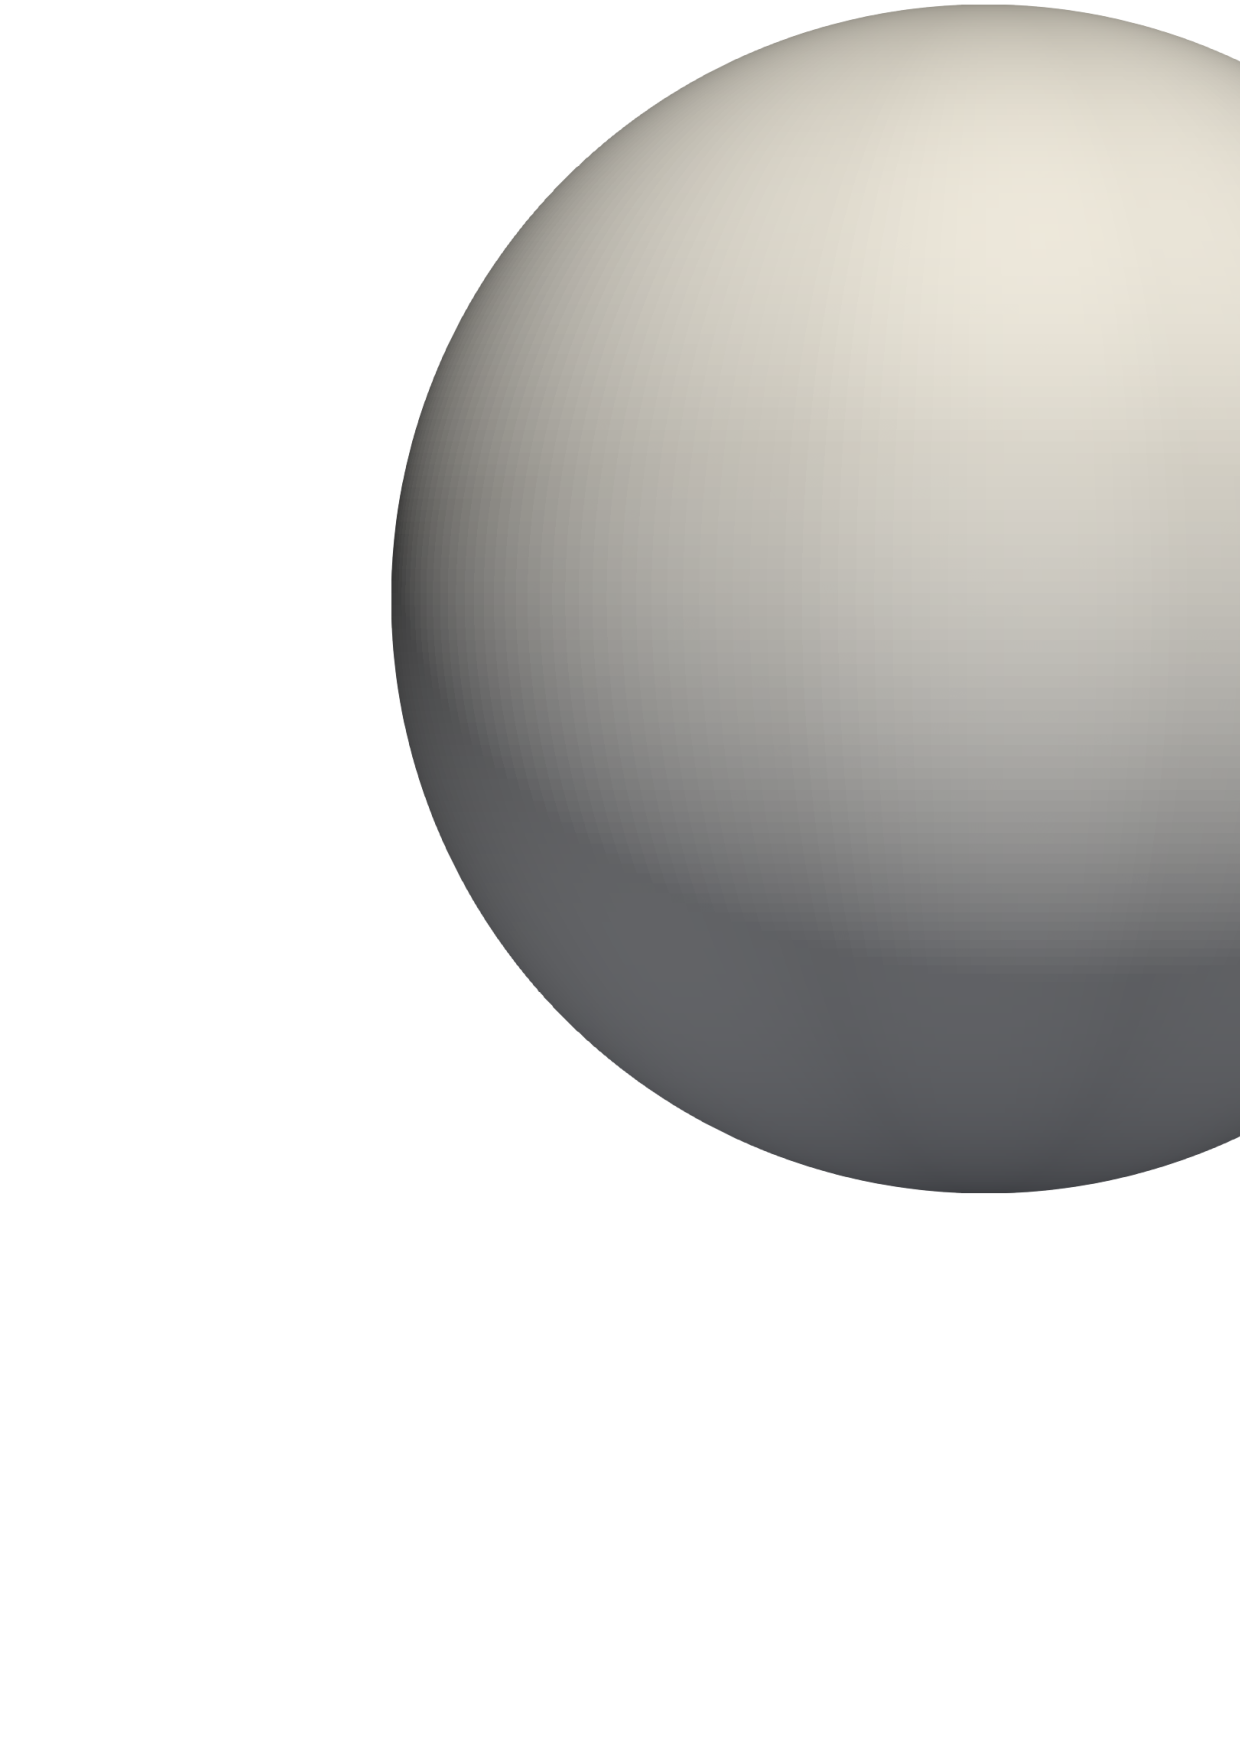
\includegraphics[width=\textwidth]{chap_8_fig_6.pdf}
\caption{Spontaneous self-organization of a polarized ``cell migration'' mode in an active gel with a non-monotonic dependence of active tension and nematic activity on cortical density.}
\label{fig_5_III}
\end{figure} 

To trigger the symmetry-breaking instability, we introduced in the initial state a random fluctuation in cortical density with maximum amplitude of 1\%. Above a threshold activity, the system develops a polarized ``cell-motility'' mode, Fig.~\ref{fig_5_III} and \href{https://github.com/waleedmirzaPhD/movies_thesis.git}{Movie~7.4}. The retrograde flow establishes a stable cortical density gradient towards the cell rear. As active tension and nematic activity are not a monotonic function of cortical thickness, their maxima  develop somewhere between the front and the rear of the cell, where a band of enhanced order develops. Since $\kappa>0$, this results in localized higher circumferential tension and pinching the cell into a pear shape. Thus, these results suggest that measurements of shape, cortical density and local nematic order in polarized cells may provide sufficient information to infer the dependence of active forces on density and filament alignment. %A parametric analysis of the influence of $\kappa$ on the cell shape (Fig.~\ref{fig_6_III} and Movie~$7.5$ in Appendix~\ref{appendix_2}) shows a higher value of anisotropic tension constricts the cell and creates  a thin tail-like protrusion in the rear of the cell.

%\begin{figure}[h!]
%\centering
%\vspace*{0cm}\includegraphics[width=1\textwidth]{chap_8_fig_7.pdf}
%\caption{Parametric analysis to demonstrate the influence of $\kappa$ on shape changes during cell motility. A higher value of $\kappa$ together with furrow ring-like actin architecture in the rear elongate the cell by creating constriction due to higher anisotropic contraction in the circumferential direction.}
%\label{fig_6_III}
%\end{figure} 


%The increased contractility introduces compressive hydrodynamic gradients which together with active torque align the network perpendicular to the axis of polarity forming the circumferential ring of actin network. For $\kappa>0$, the resulting anisotropy in architecture generates higher tension in circumferential direction in high-alignment region and hence locally pinching the cell into a pear shape. A parametric analysis of the influence of $\kappa$ on the cell shape (Fig.~\ref{fig_6_III} and \href{https://www.dropbox.com/s/aq3autc6uuefy2t/movie_2.3.4.mp4?dl=0}{Movie~$2.3.4$}) see Appendix~\ref{appendix_2} shows a higher value of anisotropic tension constricts the cell and creates  a thin tail-like protrusion in the rear of the cell. At higher active torque and contractility (Fig.~\ref{fig_7_III} and \href{https://www.dropbox.com/s/zdao6ix7kjil2rc/movie_2.3.5.mp4?dl=0}{Movie~$8.5$}) see Appendix~\ref{appendix_2} we observe an oscillatory motion of the tail-like protrusion whereby the rear end of the cell protrude and retract. As explained the protrusion results from higher anisotropic tension generated in the ring of actin network. This cell protrusion results in hydrodynamic extension in tail of the cell which locally aligns the fibers along the axis of polarity. This in turn allows the network to generate tension and retract the extrusion forward. The forward motion of the tail once again generates a compressive hydrodynamic gradient aligning fibers circumferentially and hence generating a sustained cycle of extrusion and retraction of the cell's rear-end. Lastly, it is imperative to reiterate that assuming contractility as linear or saturating Hill–Langmuir function of $\rho$ does not reproduce the shape changes or network architecture observed in \cite{Ruprecht:2015aa}.





%\begin{figure}[h!]
%\centering
%\vspace*{0cm}\includegraphics[width=1\textwidth]{chap_8_fig_7.pdf}
%\caption{Parametric analysis to demonstrate the influence of $\kappa$ on shape changes during cell motility. A higher value of $\kappa$ together with furrow ring-like actin architecture in the rear elongate the cell by creating constriction due to higher anisotropic contraction in the circumferential direction.}
%\label{fig_6_III}
%\end{figure} 
%
%\begin{figure}[h!]
%\centering
%\vspace*{0cm}\includegraphics[width=0.8\textwidth]{chap_8_fig_8.pdf}
%\caption{Sequence of events involving self-organization of actin nematic architecture on a cortical surface due to a north-south pole symmetry breaking at a relatively higher activity of the bundling proteins. The shape changes result from an interplay between actin flow to the rear of the cell and periodic oscillations of actin network alignment between the polarity axis and in the normal direction to the polarity axis. The length and direction of the red segment indicate nematic order parameter $S$ and $\bm{n}$ respectively. Movie~corresponding to this figure can be accessed here \href{https://www.dropbox.com/s/zdao6ix7kjil2rc/movie_2.3.5.mp4?dl=0}{movie~$8.5$} see Appendix~\ref{appendix_2}}
%\label{fig_7_III}
%\end{figure} 




\section{Summary}

In this chapter, we have particularized the theory for active nematic gels on deformable surfaces proposed in Chapter~\ref{chap_7} to axisymmetry. We have also developed a fully discrete numerical formulation based on a time-incremental Onsager principle and a B-Spline finite element discretization. This approach grants very fast fully nonlinear simulations of the dynamics coupling  cytoskeletal density, nematic order, and surface shape. We have focused on cell division and polarized cellular states, for which axisymmetry is a reasonable assumption.

Our results support the notion that increased equatorial contractility leads to the self-organization of a high-density band with high alignment that efficiently constricts the cell \cite{anne2016}. Our results further show that the nematic coupling significantly affects previous results about the biophysics of cell division. More specifically, we find that nematic coupling reduces the threshold of equatorial over-activity required to complete division, and significantly accelerates the process. Furthermore, in the absence of equatorial over-activity, we show in the fully nonlinear regime that beyond a base activity, the system develops a symmetry-breaking cytokinetic-like instability leading to cell division as previously suggested \cite{mietke2019_2}. Thus, on top of biologically controlled equatorial  overactivity \cite{spira2017}, self-organization can contribute to robust cell division. We also show that our model can develop polarized motility-like instabilities with cellular shapes similar to those  observed experimentally \cite{Ruprecht:2015aa} that depend on how active tension is modulated by density and nematic order. 

%Lastly, the solution of the proposed model in the axisymmetric setting is very limited in terms of exploring relevant biological systems. The literature review in Chapter~(\ref{chap_6}) indicates that several biological surfaces such as a vesicle or an epithelial layer do not abide by the constraint of axisymmetry and hence the dependence on the coordinate $\varphi$ arises. Therefore, in the next chapter, we proposed the numerical solution of the model on an arbitrary manifold and explore it in the relevant settings.







\renewcommand{\thesection}{8.\arabic{section}}
\chapter{Active shape changes in inextensible liquid crystalline vesicles}	\label{chap_9}
\section{Introduction}

In the previous chapter, we have focused on compressible active nematic gels pertinent to the sparse actin cytoskeleton, in which the mechanism of density patterning by self-reinforcing flows couples to nematic ordering. In such models,  the nematic order parameter can can vary between 0 and 1 and hence nematic order defects are not topological requirements. Other active nematic systems with high-density and/or long filaments, such as microtubule-kinesin gels, exhibit high local order everywhere except at defects, which are motile and dominate the dynamics  \cite{ndlec1997, surrey2001,sanchez2012}. Such systems are  well described by  active nematic liquid crystal (LC) theories, which commonly disregard density effects and where susceptibility parameters favor high local order \cite{zhang2018,kumar2018}. When confined to a deformable surface, liquid-crystalline systems develop orientational defects which strongly interact with local curvature, as shown in active and passive vesicles \cite{keber2014,xing2012} and during hydra morphogenesis \cite{maroudas2021}. Activity can modify the nature of defects and also induce complex dynamical states involving shape and defect reconfigurations and persistent interfacial flows. In active nematic vesicles, the bilayer where the nematic gel is confined imposes local inextensibility of the flow and provides bending resistance. 

Inextensibe active LC deformable surfaces  fall within the theoretical framework developed in Chapter~\ref{chap_7}. As discussed in the introduction of Part II of this thesis, Chapter~\ref{chap_6}, the general computational treatment of such models is challenging with only a handful of references addressing the coupled dynamics of defects and shape. To describe interfacial field theories on curved and time-evolving interfaces, there are two broad  approaches, one expressing the theories in  curvilinear coordinates adapted to the surface, and another one expressing them in Cartesian coordinates of ambient space and then projecting them on the surface. The curvilinear approach requires the language of differential geometry whereas the mathematical formulation and implementation of the Cartesian approach is simpler. However, the Cartesian approach is less efficient in that tangential fields are represented as 3D fields along with constraints. Here, we follow the curvilinear approach. To take advantage computationally of the mathematical efficiency of the curvilinear approach, one needs to approximate numerically tangent vector and tensor fields on a surface, which is not trivial because both the components and the basis vectors depend on position. Other computational challenges include the need of a smooth numerical representation of the surface, e.g.~to compute square integrable curvatures, handling large deformations and mesh distortions, or the requirement of an inf-sup compatible discretization of the Lagrange multiplier fields imposing local inextensibility. 

The rest of the Chapter is organized as follows. Section~\ref{chap8sec1}  describes the theoretical model for an active inextensible nematic fluid vesicle.  In Section~\ref{chap8sec2}, we propose a computational framework involving an efficient numerical solution of the governing equations discretized in space and time. Section~\ref{chap8sec3} explores computationally the tight interplay between dynamics of defects and curvature, first for passive vesicles with different geometric properties and then for active nematic vesicles. %In Section~\ref{chap8sec4}, we summarize our findings, outline the limitations of our approach and propose avenues for future research. 


\section{Governing equations based on Onsager's formalism}\label{chap8sec1}

We consider a thin and inextensible active nematic layer, whose shape is described by a time-evolving surface $A$ parametrized as described in Chapter~\ref{chap_7}, and whose orientational order is described by a tangential nematic tensor field, Eq.~(\ref{27_II}). The three-dimensional velocity field with tangential $\bm{v}$ and normal components $v_{N}$, i.e.~$\bm{V} = \bm{v} + v_{N}\bm{N}$, describes the interfacial flows and the rate-of-change of shape, whereas the Jaumann derivative  of the nematic tensor, $\widehat{\bm{q}}$, characterizes changes in nematic order. To impose local inextensibility, we resort to a Lagrange multiplier tension-like field $T$, whereas we enforce conservation of enclosed volume with a Lagrange multiplier pressure difference $P$.


%We characterize the rate of change of $\bm{q}$ with the Jaumann derivative $\widehat{\bm{q}}$ given by which measures the rate of change of the components of $\bm{q}$  viewed by an observer that flows and rotates with $\bm{v}$; thus, $\widehat{\bm{q}}$ is zero if $\bm{q}$ is advected and rotated by the flow without any further rearrangements of the nematic field. For a surface that is inextensible under both tension and compression. This constraint would have to be expressed by an isotropic tension field $T$. Lastly, we use pressure field $P$ to enforce the conservation of global volume due to osmotic effects.


We derive the governing equations of an active nematic system at low Reynolds numbers following non-linear Onsager's variational formalism. In this formalism, one needs to identify the free-energy of the system, $\mathcal{F}$, and the dissipation and power potentials, $\mathcal{D}$ and $\mathcal{P}$. 
The governing equations are obtained by minimizing the Rayleighian $\mathcal{R}=\dot{\mathcal{F}}+\mathcal{D}+\mathcal{P}$, where $\dot{\mathcal{F}}$ is the rate of change of the free energy.  The elastic behavior of the vesicle surface $\mathcal{F}$ is given by
\begin{equation} \label{9_1}
   \mathcal{F}[\bm{q}, \bm{x}] =\underset{A}{\int} \left(\frac{ \mathcal{B} }{2} H^{2} - \frac{a}{2}S^{2} + \frac{b}{8} S^{4} + \frac{L}{2}\nabla_c q_{ab} \nabla^c q^{ab} \right) \,d A \, ,
\end{equation}
where $H = g^{ab}k_{ab}$ is the local mean curvature. The first term above is the Helfrich bending energy of the membrane.  The second and third terms favor spontaneous nematic ordering on the membrane order parameter $S_0 = \sqrt{2a/b}$, where $a$ and $b$ are positive material constants. The last term is the Frank energy, controlled by the Frank constant $L$. Above the nematic correlation length $\ell_q = \sqrt{L/(2a)}$, the second and third terms dominates over the Frank term.

The dissipation potential is given by 
\begin{align}  \label{9_2}
    \mathcal{D}[\bm{q}, \bm{x};  \bm{V}, \widehat{\bm{q}}]   = \underset{A}{\int} \left[  \eta  d_{ab} d^{ab}+   \frac{\eta_{\text{rot}}}{2}  \widehat{q}_{ab}\widehat{q}^{ab} +\beta  d_{ab} \widehat{q}^{ab}   +  \frac{\gamma}{2} \left(v_a v^a + v_N^2\right) \right]   dA , \end{align}
where the first term is the shear dissipation potential, with $\eta$ the 2D membrane viscosity, the second term is the nematic dissipation potential, the term third captures the dissipative coupling between shear rate and changed in nematic order, and the last term models the frictional drag of the bilayer with its environments.

The power supply to the system by activity is characterized by the power potential
 \begin{align}  \label{9_3}
  \mathcal{P} \left[\bm{q}, \bm{x};  \bm{V} \right]  &=\underset{A}{\int} \lambda_{\rm ansio}q^{ab}d_{ab} dA,
 \end{align}
where $\lambda_{\rm aniso}>0$ for a contractile system and   $\lambda_{\rm aniso}<0$ for an extensile system such as microtubule-kinesin gels. We impose the inextensibility  and volume conservation using the constraint potential \begin{equation} \label{9_4}
    \mathcal{Q}\left[\bm{x};\bm{V}, T,P \right] = \underset{A}{\int}  T d^{a}_{\,a}     d A +  P \underset{A}{\int}  v_N  d A,
\end{equation}
To form the Lagrangian of the system, we need to compute the rate of change of the free-energy in Eq.~(\ref{9_1}). Because the surface is inextensible, the local changes in area and density are zero and we have the simple expression  $\mathcal{\dot{F}} =\underset{A}{\int} \mathcal{L}_{\bm{V}} f dA$.

We emphasize that these functionals intimately couple tangential flows in the fluid membrane, given by $\bm{v}$, and shape changes, given by $v_N$. Indeed, the rate-of-deformation tensor $\bm{d}$ involves these two velocities, see Eq.~(\ref{eq6:d}), and this tensor appears in each of the functionals involved in the system Lagrangian both explicitly and through the Jaumann derivative of the nematic tensor.

Particularizing the generic Euler-Lagrange equations obtained in Chapter~\ref{chap_7} to the present model, the governing equations are summarized in  Box~D. 


\begin{center}
\begin{mybox}{gray}{\center{\textbf{Box~D: Governing equations for an inextensible active nematic liquid crystalline membrane}}}
		
		\textbf{Generalized force balance for nematic field}
		\begin{equation}  \label{box_d_eq_1}
			\eta_{\text{rot}} \widehat{q}^{ab} +( 2a+bS^2 ) q^{ab} -  L\Delta q^{ab}   +\beta  d^{\textup{dev} \, ab}   = 0.
		\end{equation}
		
		\textbf{In-plane balance of linear momentum}:
		\begin{equation} \label{box_d_eq_2}
			\nabla_b \left(\sigma^{\textup{s} \, ab} + \sigma^{\textup{a} \, ab }   \right) -\sigma_N^b k^a_{~ b}= \gamma  v^a.
		\end{equation}
		
		\textbf{Out-of-plane  balance of linear momentum}:
		\begin{equation} \label{box_d_eq_3}
			\nabla_a \sigma^a_N - \sigma^{\textup{s}  \, ab} k_{ab} - \gamma v_N  + P = 0.
		\end{equation}
		
		\textbf{Constitutive relations}:
		\newline
		Power-conjugate to the rate-of-deformation tensor $d_{ab}$:
		\begin{align} \label{box_d_eq_4}
			\sigma^{\textup{s} \, ab}  =    2\eta d^{ab} -\mathcal{B}Hk^{ab}  -L\nabla^a q_{cd} \nabla^b q^{cd}    + \beta \widehat{q}^{ab}   +  \lambda_{\rm aniso} q^{ab}  . 
		\end{align}
		Power-conjugate to the in-plane and out-of-plane spins:
		\begin{align}  \label{box_d_eq_5}
			\sigma^{\textup{a} \, cd } = \frac{1}{2}\left(m^{ab} k_{ab} - \nabla_a m_N^a\right)\epsilon^{cd},
			\;\;\;\;\;\;\;\;
			\sigma_{N}^a  =- \epsilon^a_{~b} m_N^{c} k^{~b}_{c} - \epsilon^a_{~b}\nabla_c m^{cb}.
		\end{align}
		Power-conjugate to the gradients of the spins
		\begin{equation}  \label{box_d_eq_6}
			m_{N}^c= 2 L \epsilon_{fg} \nabla^c q^{af} q^g_{~a},
			\;\;\;\;\;\;\;\; m^{ab} = - \mathcal{B} Hg^{ab}.
		\end{equation}
		
		\textbf{Constraints}
		
		Incompressibility constraint:
		\begin{equation}  \label{box_d_eq_7}
			d^a_{~a} = 0.
		\end{equation}
		Balance of enclosed (incompressible) fluid:
		\begin{equation}  \label{box_d_eq_8}
			{\int_A}  v_N d A = 0.
		\end{equation}
	\end{mybox} \label{Box3}
\end{center}



\section{Numerical discretization} \label{chap8sec2}

 In this Section, we propose a method to discretize the governing equations in space and time. As in the previous chapter, we discretize spatial fields using finite elements and time using finite differences, and we derive the discrete equations from a time-discrete incremental Onsager principle, which grants nonlinear stability. One important decision when describing interfacial problems on fluid membranes is whether the parametrization follows material particles (Lagrangian parametrization) or not. A strictly Eulerian approach, such as that considered in the 2D model of Chapter \ref{chap_3}, is not meaningful for a deforming surface since surface motion is necessarily Lagrangian, but arbitrarily Lagrangian-Eulerian approaches are possible \cite{torres2019}. Here, we adopt a Lagrangian approach, which is mathematically and conceptually simple but requires remeshing algorithms to avoid excessive element distortion as a result of interfacial flows. 
 
 Space discretization of the present theory is challenging in various ways. First, because our theory involves surface curvature and Christoffel symbols, the numerical parametrization of the surface needs to be smooth, at least $C^1$ with continuous first derivatives. We consider Loop subdivision finite elements defined over triangulated surfaces. This method is an extension of splines to unstructured triangular grids, and leads to  smooth numerical surfaces. Second, we  need to choose a finite element space for the Lagrange multiplier field $T$ compatible with that of velocities. We address this by resorting to a macro-element approach adapted to subdivision approximations.  Third, we need to develop an efficient approximation for the traceless and symmetric tangential nematic field over a curved surface.  
 
 \subsection{Space discretization}

%We note that our model involves functionals that depend on curvature tensors and Christoffel  symbols. As a result, they contain second-order derivatives of fields and hence the finite-element solution requires $C^1$ interpolation. In particular, to ensure the energy is finite, the shape functions, as well as their first and second derivatives, should be square-integrable. For this reason, we use a higher-order Loop subdivision basis function on triangulated surfaces, guaranteed to be $C^2$ continuous everywhere except in the vicinity of irregular points where they are $C^1$ continuous. At the highest level of description, we may say that subdivision schemes construct smooth surfaces through a limiting procedure of repeated refinement starting from an initial mesh. This initial mesh will also be referred to as the control mesh of the surface. Generally, subdivision schemes consist of two steps. First, the mesh is refined, e.g., all faces are quadrisected, followed by the computation of new nodal positions. These positions are simple, linear functions of the nodal positions of the coarser mesh. These computations are local,i.e., they involve only nodal positions of the coarser mesh within a small, finite topological neighborhood, leading to very efficient implementations. Using a suitable choice of weights, such subdivision schemes can be designed to produce a smooth surface in the limit. Subdivision methods which result in limit surfaces whose curvature tensor is square-integrable are especially appealing for geometrical modeling applications and for thin-shell analysis.

\subsubsection*{Numerical approximation of kinematics}

Subdivision surfaces is a technology originally developed in computer graphics to numerically represent smooth surfaces, which was later adapted to the finite element context to solve thin shell and other interfacial partial differential equations  \cite{loop1987,stam1998,cirak2000,cirak2011,torres2019}. The discrete surface is represented by a surface triangulation, called control mesh, with $E= 1,....,N_e$ triangular elements and $I= 1,....,N_n$ nodes or vertices with position vector $\bm{x}_I\in\mathbb{R}^3$. The vertices are called control points. The method provides a prescription to define time-dependent element-wise local parametrizations of the form
\begin{equation} \label{9_17}
    \bm{x}= \bm{\phi}^E(\bm{\xi},t)= \underset{I \in R^E}{\mathrm{\sum}} B_I(\bm{\xi})\bm{x}_I(t),
\end{equation} 
where $R^E$ denotes the set of nodes belonging to element $E$ and to the first ring of elements adjacent to element $E$,  $B_I$ are the Loop subdivision basis functions defined over a reference triangular domain with coordinates $\bm{\xi} = (\xi^1, \xi^2)$, and $\bm{x}_I(t) = x^A_I(t) \bm{i}_A$ is the time-dependent position of vertex $I$ expressed in a Cartesian basis of $\mathbb{R}^3$. See Fig.~\ref{fig_1}(a) for an illustration. A vertex on the mesh is said to be regular if it is connected to exactly six other vertices on the triangulation. If all nodes of element $E$ are regular, then $B_I$ are explicitly known cubic box splines. Otherwise, their calculation is more involved.   

At any given time, the image of the reference triangular domain by the local chart $\bm{\phi}^E(\bm{\xi},t)$ is a curved triangle, which we denote by $A^E$. The subdivision method guarantees that these curved triangles do not overlap and that their union  $A = \bigcup_{E=1}^{N_e} A^E$ is regular surface, $C^2$ continuous everywhere except at irregular points where it is $C^1$.


\begin{figure}
	\centering
	\hspace*{-0.5cm}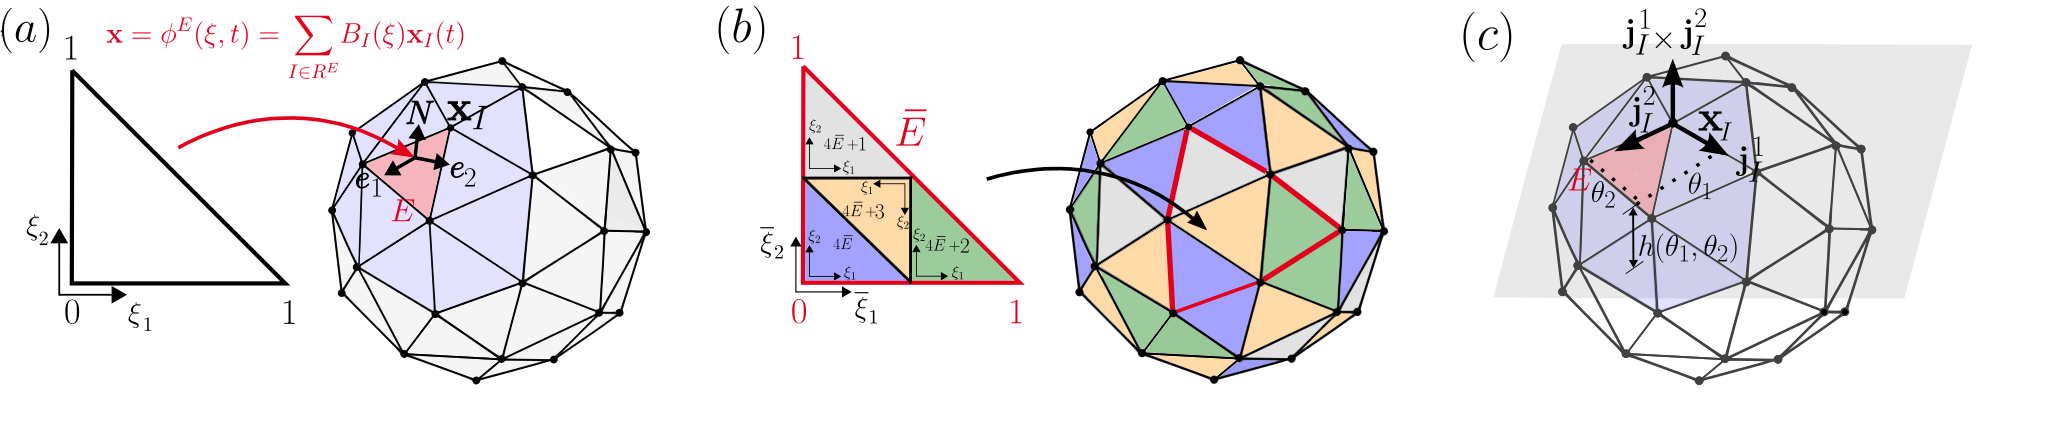
\includegraphics[width=1.\textwidth]{fig_sec_2_chap_4_1_1.pdf}
	\caption{\textbf{Illustration of space discretization.}  (a) Element-wise parametrization of the surface, $\bm{\phi}^E(\xi^1, \xi^2, t)$, using subdivision basis functions from a fixed reference domain. This local parametrization on a given element (shaded in red) depends on the nodes belonging to the one-ring of elements surrounding it (shaded un blue). (b) Nested meshes required to construct an inf-sup compatible discretization. Positions and velocities are approximated on the fine mesh, whereas the Lagrange multiplier field $T$ imposing local inextensibility is approximated on the coarse mesh. The figure also illustrates the correspondence between the reference coordinates of coarse and refine elements. (c) A local Monge parametrization of the surface, $\bm{\varphi}^I(\bm{\theta})$, is defined around each vertex $I$ in the mesh in terms of the height of a point in the surface $h(\bm{\theta})$ relative to a plane tangent to the surface at that vertex. This parametrization is expressed in terms of Cartesian coordinates of the plane $(\theta^1, \theta^2)$. To establish a correspondence between the multiple element-wise parametrizations $\bm{\phi}^E(\bm{\xi},t)$ of elements adjacent to vertex $I$, we build diffeomorphisms $\bm{\xi} = (\bm{\phi}^E)^{-1} \circ \bm{\varphi}^I (\bm{\theta})$ mapping the common local Monge coordinates to those of each of the adjacent elements.} 	%	A closed surface $A$ approximated with union of subdivision triangular elements $A_{\{K\}}$, i.e, $A = \bigcup_{K=1}^{N_e} A_{E_{\{K\}}}$. A material point $\bm{x}$ in element $E_{\{K\}}$ on the surface is approximated using map in Eq.~(\ref{9_17}) with control points $\bm{x}_K$ belonging to the first ring of the surrounding elements $\langle E_{\{K\}} \rangle$. (b)  A closed surface $A$ approximated with union of subdivision triangular elements $A_{E_{\{J\}}}^m$, i.e, $A = \bigcup_{L=1}^{N_e^m} A_{E_L}^m$. Each element $E_L^m$ can be formed by local coarsening (or union) of four adjacent elements of the velocity mesh, i.e,  $(4E^m_{\{J\}}, 4E^m_{\{J\}}+1, 4E^m_{\{J\}}+2, 4E^m_{\{J\}}+3)$ and therefore $ N_e= 4N_e^m$. The mapping between the parametric coordinates $\bm{\psi}$ and $\bm{\psi}^m$ is given by set of Eqs.~(\ref{9_24}). (c) Local monge parametrization of an arbitrary order tensor on material point $\bm{x}$ in the tangent space of $A_J$ requires basis  $ (\bm{j}_I^1,\bm{j}_I^2,\bm{j}_I^3)$ of the neighbouring control points $\bm{x}_{\{K\}}$ and a transformation tensor $T_{[\phi,\varphi]~a}^{\quad \,\, A}$ that establish a map between the local monge basis $\bm{B}_{\varphi_I} = \{\partial_A \bm{\varphi}_I\}$ and local basis $\bm{B}_{\phi} = \{\partial_a \bm{\phi}\}$ at point $\bm{x}$. Note that, in this figure for simplicity we ignored the tilde $\sim$ notation.}
	\label{fig_1}
\end{figure} 


Given this collection of $N_e$ local parametrizations,  quantities defined in Chapter \ref{chap_7} such as the tangent vectors $\bm{e}_a$, the metric tensor and second fundamental form components, $g_{ab}$ and $k_{ab}$, or the Christoffel symbols $\Gamma^c_{\,ab}$, can be computed in each element. For instance, the metric tensor in element $E$ follows from $g_{ab} = \partial_a \bm{\phi}^E \cdot  \partial_b \bm{\phi}^E$ where $\partial_a$ denotes partial differentiation with respect to $\xi^a$. Since our description of motion is Lagrangian, the membrane velocity can be computed simply by time-differentiation of Eq.~(\ref{9_17}) as 
\begin{equation} 
    \bm{V}(\bm{\xi},t)= \partial_t\bm{\phi}^E(\bm{\xi},t)= \underset{I \in R^E}{\mathrm{\sum}} B_I(\bm{\xi})\dot{\bm{x}}_I(t),
\end{equation} 
which allows us to compute the normal and tangential components as $v_N = \bm{V} \cdot \bm{N}$ and $\bm{v} = \bm{V} - v_N \bm{N}$. In the Lagrangian setting, the rate-of-deformation tensor can also be computed from partial differentiation of the metric tensor at fixed Lagrangian coordinate as $d_{ab} = \frac{1}{2}\partial_t g_{ab}$.




%Assume $\bm{x}$ presents material points on a discrete time evolving closed surface $A$ which is formed  by a collection of triangulated finite element parametrization. To define the discretization of a generic surface $A$ with loop subdivision basis function \cite{loop1987,stam1998,cirak2000,cirak2011,torres2019}, we consider a control mesh made of triangles $E_{\{J\}}$ where $J= 1,....,N_e$ whose edges join the set of control points with coordinates  $\bm{x}_{\{I\}}$ where $I= 1,....,N_n$. A Lagrangian map on $A$ in element $E_{\{K\}}$ is given as
%\begin{equation} \label{9_17}
%    \bm{x}= \phi(\bm{\psi})= \underset{K \in \langle E_{\{K\}} \rangle}{\mathrm{\sum}} B^{\rm s}_{\{K\}}(\bm{\psi})\bm{x}_{\{K\}},
%\end{equation} 
%where $\bm{x}_{\{K\}}$ are the coordinates of the $K-$th control point, $B^{\rm s}_{\{K\}}$ are Loop subdivision basis functions and $\langle E_{\{K\}} \rangle$ refers to the control points contributing to the approximation of $\bm{x}$ in element $E_{\{K\}}$. We denote a triangle obtained by the local parametrization Eq.~(\ref{9_17}) as $A_{E_{\{K\}}}$. The discrete surface $A$ is given by the union of the curved triangular elements as $A = \bigcup_{K=1}^{N_e} A_{E_{\{K\}}}$. The local basis functions are given by the first derivative of the subdivision basis function as
%\begin{equation}  \label{9_18}
%    \bm{e}_{a} (\bm{\psi})=  \frac{ \partial \bm{x}}{\partial \psi_a } = \underset{K \in \langle E_{\{K\}} \rangle}{\mathrm{\sum}} \partial_{a} B^{\rm s}_{\{K\}} (\bm{\psi}) \bm{x}_{\{K\}}.
%\end{equation}
%where $\partial_a (\bullet)  = \partial  (\bullet) /\partial \psi_a$.
%The components of discrete metric tensor are given by $g_{ab} = \bm{e}_{a} \cdot \bm{e}_{b}$ and its inverse is given as $\{g^{ab}\} = \bm{g}^{-1}$. The discrete curvature tensor is given by the second derivative of the subdivision basis function 
%\begin{equation} \label{9_19}
%     k_{ab} = -\bm{N} \cdot  \partial_a  \partial_b \bm{x},
%\end{equation}
%where
% $\bm{N} = (\bm{e}_1 \times \bm{e}_2)/\left|\bm{e}_1 \times \bm{e}_2 \right|$.
% The discrete matrix of Christoffel  symbols 
% $\Gamma^c_{\,ab}$ is given as 
%\begin{equation} \label{9_20}
%    \Gamma^c_{\,ab} = \frac{1}{2}g^{cd}\left( \partial_a g_{bd} + \partial_b g_{ad} - \partial_d g_{ba} \right),
%\end{equation}
%where
%\begin{equation} \label{9_21}
%\partial_a g_{bd} = \partial_a \bm{e}_b \cdot \bm{e}_d + \bm{e}_b  \cdot \partial_a \bm{e}_d.
%\end{equation}
% The evolution of surface $A$ is given by the velocity field $\bm{V} = v^a \bm{e}_a + v_N \bm{N}$. As the basis vectors  $\bm{e}_a$ depend on the local coordinates therefore their inclusion can lead to discontinuous velocity fields across the element boundary. A better alternative is to discretize the cartesian components of the discrete velocity field, i.e,  $\bm{V}=V^A \bm{i}^A$, where $V^A$ is given as 
%\begin{equation} \label{9_22}
%    V^A = \underset{K \in \langle E_{\{K\}} \rangle}{\mathrm{\sum}} B^{\rm s}_{\{K\}}(\bm{\psi})V^A_{\{K\}},
%\end{equation}
%\marino{[Is it true that $d \bm{x}_{\{K\}}/dt = V^A_{\{K\}}$??]}
%The rate at which the surface $A$ deforms both in-plane and out-of-plane is given by the discrete rate of change of deformation tensor $\bm{d}$. In Lagrangian parametrization the rate of change of deformation tensor is simply estimated as
%\begin{equation} \label{9_23}
%    d_{ab} = \frac{ \partial g_{ab}}{ \partial t}.
%\end{equation}



\subsubsection*{Lagrange multipliers}

When imposing local incompressibility through a field of Lagrange multipliers, here the surface tension field $T$, it is well-known that the approximation spaces of velocities and Lagrange multipliers need to be compatible and satisfy the so-called inf-sup condition \cite{brezzi2012}. This condition is required to prove convergence and avoids locking or spurious oscillations in the Lagrange multiplier field. Essentially, it expresses at a discrete level that all scalar fields can be expressed as the divergence of a vector field. Finding inf-sup compatible discretizations is delicate and depends on the specific approximation space.

In the context of spline-based approximations, \citet{dortdivanlioglu2018} exploited the refinement property of B-splines, according to which the approximation space in a given grid is nested in that of a refined grid. This reference shows that in bulk problems, an inf-sup compatible approximation is obtained by choosing the refined approximation space for positions or velocities and the coarser space for Lagrange multipliers. This kind of approach falls within the category of macro-element methods. Since subdivision surface approximation spaces also have such refinement property, we adopt this approach to the present surface setting. This macroe-element method for subdivision approximations was previously tested in 2D and in problems dealing with reshaping coupled to inextensible interfacial hydrodynamics  \cite{torres2019}.

We thus consider a pair of subdivision approximations based on nested triangulations defined by refinement of each element in the coarse grid into four elements in the refined grid, Fig.~\ref{fig_1}(b). The coarse mesh has $\bar{N}_e$ elements with $N_e = 4\bar{N}_e$. We approximate the surface tension field $T$ over the coarse mesh using its associated subdivision basis functions. Within element $E$ of the coarse mesh, 
\begin{equation} \label{discr_T}
    T(\bar{\bm{\xi}},t)=  \underset{I \in \bar{R}^E}{\mathrm{\sum}} \bar{B}_I(\bar{\bm{\xi}})T_I(t),
\end{equation} 
where $\bar{\bm{\xi}}$ are the parametric coordinates of an element in the coarse mesh, $\bar{R}^E$ is the set of nodes in the coarse mesh belonging to the first ring of elements around element $E$, $\bar{B}_I(\bar{\bm{\xi}})$ are the subdivision basis functions of the coarse mesh, and $T_I(t)$ are the time-dependent coefficients associated to control points of the coarse mesh. 

The constraint functional in Eq.~(\ref{9_4}) is an integral whose integrand involves the product of $T(\bar{\bm{\xi}},t)$ and the rate-of-deformation tensor computed in terms of $\bm{V}(\bm{\xi},t)$. Thus, in the finite element implementation, where such integrals are performed element by element with numerical quadrature, we need a map between the coordinates of the reference element for the coarse mesh $\bar{\bm{\xi}}$ and the coordinates in each of the corresponding four elements of the refined mesh, Fig.~\ref{fig_1}(b). This map is explicit and given by
\begin{align} 
& \bar{\xi}^a<\frac{1}{2}, & \textup{corresponds to refined element 1 and}\; &  \xi^a = 2\bar{\xi}^a, \nonumber \\
& \bar{\xi}^1>\frac{1}{2}, \, \bar{\xi}^2<\frac{1}{2}, & \textup{corresponds to refined element 2 and}\; & \xi^1 = 2\left(\bar{\xi}^1-\frac{1}{2}\right) , \, \xi^2 = 2\bar{\xi}^2 , \nonumber \\
& \bar{\xi}^1<\frac{1}{2}   , \,\bar{\xi}^2>\frac{1}{2}, & \textup{corresponds to refined element 3 and}\; & \xi^1 = 2\bar{\xi}^1,\, \xi^2 = 2\left(\bar{\xi}^2-\frac{1}{2}\right) , \nonumber \\
& \bar{\xi}^1 + \bar{\xi}^2>\frac{1}{2},~  \bar{\xi}^1<\frac{1}{2}, & \textup{corresponds to refined element 4 and}\; & \xi^a = 1-2\bar{\xi}^a.\nonumber  
\end{align}


%
%
%
%We use a  discrete surface tension field $T(\bm{x},t)$ as a Lagrange multiplier to impose the incompressibility constraint. To approximate $T(\bm{x},t)$, we use a discrete mesh that satisfies the inf-sup condition \cite{brezzi2012} to ensure stability of the solution. For this purpose, we use the macro-element approach \cite{dortdivanlioglu2018} where the surface tension field is discretized on a coarsened mesh. Consider a mesh with triangular elements $E^m_{\{J\}}$ where $J= 1 ... N_e^m $ such that $N_e = 4N_e^m$. We subdivide each triangle in four triangles, i.e, $(4E^m_{\{J\}}, 4E^m_{\{J\}}+1, 4E^m_{\{J\}}+2, 4E^m_{\{J\}}+3)$. Given $(\psi_1^m,\psi_2^m)$ are the parametric coordinates of the subdivision surface basis functions $B^m_{\{J\}}$ used to approximate $T(\bm{x},t)$, a map between mesh composed with $E_{\{J\}}$ and $E^m_{\{J\}}$ is established locally at the level of the parametric coordinates as 
%\begin{align} \label{9_24}
%\begin{split}
%   & \textup{For element $4E^m_{\{J\}}$:~~~~~} \,\,\, \psi_i = 2\psi_i^m \, \textup{where} \, \psi_i^m<\frac{1}{2}, \\ &
%    \textup{For element $4E^m_{\{J\}}+1$: } \psi_1 = 2(\psi_1^m-\frac{1}{2}) , \, \psi_2 = 2\psi_2^m   \, \textup{where } \psi_1^m>\frac{1}{2}, \, \psi_2^m<\frac{1}{2},  
%   \\  & \textup{For element $4E^m_{\{J\}}+2$: }  \psi_1 = 2\psi_1^m,\, \psi_2 = 2(\psi_2^m-\frac{1}{2}) \, \textup{where } \psi_1^m<\frac{1}{2}   , \,\psi_2^m>\frac{1}{2} , \\&
%       \textup{For element $4E^m_{\{J\}}+3$: }  \psi_i = 1-2\psi_i^m \, \textup{where}~ \psi_1^m + \psi_2^m>\frac{1}{2},~  \psi_1^m<\frac{1}{2}.
%\end{split}
%\end{align}
%The finer mesh is used to discretize $\bm{x}$ in Eq.~(\ref{9_17}),  $\bm{V}$ in Eq.~(\ref{9_22}) and the coarser mesh is used to discretize the surface tension field as follows
%\begin{equation} \label{9_25}
%    T  = \underset{K \in \langle E^m_{\{K\}} \rangle}{\mathrm{\sum}} B_{\{K\}}^m(\bm{\psi}^m) T_{\{K\}}.
%\end{equation}


\subsubsection*{Nematic order tensor}

The nematic tensor is a traceless symmetric $2\times 2$ tensor defined over the tangent space to the surface. As further elaborated by \citet{torres2020}, the approximation of tangential vector and tensor fields on surfaces is not obvious. An approximation of its components of the kind 
\begin{equation} \label{naive_B_q}
  q_{ab}(\bm{\xi},t)= \underset{I \in R^E}{\mathrm{\sum}} B_I(\bm{\xi}) q_{ab}^I(t)
\end{equation} 
is not meaningful because the nodal coefficients $q_{ab}^I$ participate in the approximation in all elements adjacent to vertex $I$, and in each of these elements these components refer to basis vectors $\bm{e}_a = \partial_a \bm{\phi}^E$ that are not only position-dependent, but also discontinuous across elements. To resolve this issue, \citet{torres2020} proposed a local Monge parametrization approach summarized below and illustrated in Fig.~\ref{fig_1}(c). 

The idea is to define around each vertex $I$  a local Monge parametrization of the surface providing a common set of curvilinear coordinates to all curved elements adjacent to $I$. To define the local Monge parametrization, we consider a plane tangent to the surface at $I$ and an orthonormal basis on this tangent plane given by vectors $\bm{j}_1^I$ and $\bm{j}_2^I$. The local Monge parametrization around vertex $I$ is then given by
\begin{equation}\label{9_27}
     \bm{\varphi}^I (\theta^1,\theta^2) =  \bm{x}_I + \theta^1 \bm{j}_1^I +  \theta^2\bm{j}_2^I + h^I(\theta^1,\theta^2) (\bm{j}_1^I \times \bm{j}_2^I),
\end{equation}
where the height function $h^I(\theta^1,\theta^2)$ measures the distance between the point on the surface along the normal to the plane from point $\bm{x}_I + \theta^1 \bm{j}_1^I +  \theta^2\bm{j}_2^I$ on the plane. The diffeomorphisms  $\bm{\theta} = \bm{\psi}^{I,E}(\bm{\xi}) =  (\bm{\varphi}^I)^{-1} \circ \bm{\phi}^E (\bm{\xi})$ map the curvilinear coordinates of each of the adjacent elements to the common local Monge  curvilinear coordinates. Hence, these changes of variables allow us to transform tensor components expressed in the finite element curvilinear coordinates of each element to tensors components expressed in the common Monge curvilinear coordinates, 
\begin{equation} \label{9_28}
\bm{q}(\bm{\xi}) = q_{ab}(\bm{\xi})\; \bm{e}^a(\bm{\xi}) \otimes \bm{e}^b(\bm{\xi}) = q_{AB}\circ\bm{\psi}^{I,E}(\bm{\xi}) \; \bm{E}^A\circ\bm{\psi}^{I,E}(\bm{\xi}) \otimes \bm{E}^B\circ\bm{\psi}^{I,E}(\bm{\xi}), 
\end{equation}
where $\bm{e}^a(\bm{\xi})$ are the dual basis vectors of $\bm{e}_a(\bm{\xi}) = \partial_a \bm{\phi}^E(\bm{\xi})$ and $\bm{E}^A(\bm{\theta}) $ are the dual basis vectors of $\bm{E}_A(\bm{\theta}) = \partial_A\bm{\varphi}^I(\bm{\theta})$ and it is implied in the notation that components referring to element-wise parametrizations have lower-case indices and components referring to the Monge parametrization around vertex $I$ have upper-case indices. In the following, we omit the composition with $\bm{\psi}^{I,E}(\bm{\xi})$ to simplify the notation.

Since $\bm{\phi}^E = \bm{\varphi}^I \circ \bm{\psi}^{I,E}$, by the chain rule we find that 
\begin{equation} \label{9_30}
    \bm{e}_a = {\left[T^{I,E}\right]^A}_a \bm{E}_A ,\quad  
     \bm{E}_A = {\left[\widehat{T}^{E,I}\right]^a}_A \bm{e}_a,
\end{equation}
where $T^{I,E}$ is the derivative of the map $\bm{\psi}^{I,E}$ and $\widehat{T}^{E,I}$ its inverse. This approach is practical and easy to implement because the components of $T^{I,E}$ are independent of the height function and explicitly available as \cite{torres2020}
\begin{equation} 
{\left[T^{I,E}\right]^A}_a = \bm{j}_A^I \cdot \partial_a \bm{\phi}^E.
\end{equation}
Dual vectors transform according to 
\begin{equation} \label{9_3030}
    \bm{e}^a = {\left[\widehat{T}^{E,I}\right]^a}_A \bm{E}^A ,\quad  
     \bm{E}^A = {\left[T^{I,E}\right]^A}_a \bm{e}^a,
\end{equation}
where we note that all quantities depend on position.

Now, to solve the issues with the approximation in Eq.~(\ref{naive_B_q}), we consider as degrees of freedom associated to vertex $I$ the components of the nematic tensor in the common Monge curvilinear coordinates $q_{AB}^I$. These coefficients define a tensor field on the surface around vertex $I$ given by 
\begin{equation} \label{9_30}
\bm{q}^I(\bm{\xi}) = q_{AB}^I \; \bm{E}^A \otimes \bm{E}^B = q_{AB}^I {\left[T^{I,E}\right]^A}_a {\left[T^{I,E}\right]^B}_b \; \bm{e}^a \otimes \bm{e}^b,
\end{equation}
where we have used Eq.~(\ref{9_3030}). We note that despite the fact that the expression in the right-hand-side involves basis vectors and transformation matrices that are discontinuous across element sides, their product represents a continuous tensor across the elements adjacent to vertex $I$ by definition since $\bm{E}^A\circ\bm{\psi}^{I,E}(\bm{\xi})$ are continuous across elements. Consequently, within each element $E$ adjacent to vertex $I$, averages of such tensor fields associated to element vertices weighted by the subdivision surface basis functions define a globally smooth nematic tensor approximations of the form
\begin{equation} \label{good_B_q}
  \bm{q}(\bm{\xi},t)= \underset{I \in R^E}{\mathrm{\sum}} B_I(\bm{\xi})  \bm{q}^I(\bm{\xi},t)= \underset{I \in R^E}{\mathrm{\sum}} B_I(\bm{\xi}) q_{AB}^I(t) {\left[T^{I,E}\right]^A}_a {\left[T^{I,E}\right]^B}_b \; \bm{e}^a \otimes \bm{e}^b ,
\end{equation} 
or in components 
\begin{equation} \label{good_B_q2}
  q_{ab}(\bm{\xi},t)= \underset{I \in R^E}{\mathrm{\sum}} \underbrace{B_I(\bm{\xi}) {\left[T^{I,E}\right]^A}_a {\left[T^{I,E}\right]^B}_b }_{{\mathcal{B}_I}_{,ab}^{AB}(\bm{\xi})} q_{AB}^I(t),
\end{equation} 
where ${\mathcal{B}_I}_{,ab}^{AB}(\bm{\xi})$ can be interpreted as generalized tensorial basis functions and the time-dependent nodal degrees of freedom are the Monge components $q_{AB}^I(t)$.

The tensor field approximation described above can be applied to general tensors. However, $\bm{q}$ is symmetric and traceless, and hence $q_{AB}^I = q_{BA}^I$ and $q_{AB}^I G^{AB} = 0$, where the inverse metric tensor coefficients $G^{AB}$ refer to the local Monge parametrization. Recalling Eq.~(\ref{9_3030}), these metric coefficients of the Monge parametrization can be computed in terms of those in the element-wise parametrizations as $G^{AB} = {\left[T^{I,E}\right]^A}_a {\left[T^{I,E}\right]^B}_b g^{ab}$. Requiring these conditions to the the tensor fields associated to vertices ensures that the finite element approximation is symmetric and traceless because a linear combination of symmetric and traceless tensors is symmetric and traceless. Hence, we can parametrize the vertex-associated tensor fields using two nodal degrees of freedom only, $q_{1}^I$ and $q_{2}^I$ as 
\begin{align}
\{q_{AB}^I\} = &
\left(\begin{array}{cc}
q_{1}^I & q_{2}^I \\
q_{2}^I  & - \frac{G^{11}}{G^{22} }q_{1}^I - 2\frac{G^{12}}{G^{22} }q_{2}^I 
\end{array}\right) 
\\ = & q_{1}^I 
\left(\begin{array}{cc} 
1 & 0 \\ 
0  & - \frac{G^{11}}{G^{22} }  
\end{array}\right) 
+ q_{2}^I
\left(\begin{array}{cc}
0 & 1 \\
1  &  - 2\frac{G^{12}}{G^{22}}  
\end{array}\right) = 
\{ L^C_{AB} q_{C}^I \}, \nonumber
\end{align}
where 
\begin{equation}
\{ L^1_{AB}\} = \left(\begin{array}{cc} 
1 & 0 \\ 
0  & - \frac{G^{11}}{G^{22} }  
\end{array}\right) , \;\;\; \mbox{and} \;\;\; \{ L^2_{AB}\} = \left(\begin{array}{cc}
0 & 1 \\
1  &  - 2\frac{G^{12}}{G^{22}}  
\end{array}\right).
\end{equation}
Hence, combining this representation of symmetric and traceless tensors with Eq.~(\ref{good_B_q2}), we finally obtain the following approximation for the components of the nematic tensor in each element
\begin{equation} \label{good_B_q2}
  q_{ab}(\bm{\xi},t)= \underset{I \in R^E}{\mathrm{\sum}} \underbrace{B_I(\bm{\xi}) {\left[T^{I,E}\right]^A}_a {\left[T^{I,E}\right]^B}_b L^C_{AB}}_{{\mathcal{B}_I}_{,ab}^{C}(\bm{\xi})} q_{C}^I(t),
\end{equation} 
where ${\mathcal{B}_I}_{,ab}^{C}(\bm{\xi})$ are generalized tensorial basis functions and the time-dependent nodal degrees of freedom are  $q_1^I(t)$ and  $q_2^I(t)$.

Given this approximation, the element-wise calculation of the covariant derivative of the nematic tensor
\begin{equation} \label{9_34}
\nabla_c q_{ab} = \partial_c q_{ab} - \Gamma^d_{~ca} q_{db} - \Gamma^d_{~cb} q_{ad},
\end{equation}
becomes a lengthy but straightforward exercise. 

%\clearpage
%
%\marino{[In what follows of this section, please check my equations with the original ones below, there were some typos, notably in matrix $L$. Also, do you think the calculations of $\nabla\bm{q}$ and $\hat{\bm{q}}$ is required?]}
%
%The traceless nematic tensor on the surface  discrete nematic order tensor in covariant formulation is defined as
%\begin{equation} \label{9_26}
%    q_{ab} = S\left(n_a n_b - \frac{g_{ab}}{2}\right),
%\end{equation}
%where $\bm{n}$ is average orientation of molecules on the vesicle surface. $S=\sqrt{2q_{ab}q^{ab}}$ represents local deviation of molecules about average orientation $\bm{n}$. As explained previously, defining a tensor field such as $ q_{ab}$ in tangent space of $A$ is an open problem due to its dependence on continuity of the local basis $\bm{e}_a$. An alternative is to discretize the cartesian components of the tensorial quantities but this can introduce extra-degrees of freedom and will render the numerical model computationally expensive. As a solution to this challenge, we employ the Local Monge parametrization proposed in \cite{torres2020}. This framework can be used to discretize a tensor with arbitrary order on a generic surface. Here we employ this framework to approximate the nematic order tensor in Eq.~(\ref{9_26}). For this purpose we introduce  an atlas of local Monge characterizations, one per vertex of the control mesh. On each vertex, we draw a plane  $\Theta$ such that there is a $1-1$ map between the $A$ and $\Theta$. We define orthonormal basis of Euclidean space in $\bm{\Theta}$ denoted by $(\bm{j}_{\{I\}}^1,\bm{j}_{\{I\}}^2,\bm{j}_{\{I\}}^3)$. The local monge parametrization around vertex $I$ can be now given as
%\begin{equation}\label{9_27}
%     \bm{\varphi}_{\{I\}} (\theta^1,\theta^2) =  \bm{x}_{\{I\}} + \theta^1 \bm{j}_{\{I\}}^1 +  \theta^2\bm{j}_{\{I\}}^2 + h_{\{I\}}(\theta^1,\theta^2)\bm{j}_{\{I\}}^3,
%\end{equation}
%where the function $h_{\{I\}}(\theta^1,\theta^2)$ gives  the height between $A$ and $\Theta$. We have two set of tangent basis; first set introduced with local monge parametrization corresponding to each node $I$, i.e, $\bm{B}_{\varphi_I} = \{\partial_A \bm{\varphi}_I\}$ and corresponding to each element $E$, i.e, $\bm{B}_{\phi} = \{\partial_a \bm{\phi}\}$. Here $\partial_A \bm{\varphi}_{\{I\}} = \bm{j}^A_{\{I\}} + \partial h_{\{I\}}/\partial \theta^A \bm{j}_{\{I\}}^3$ denotes partial differentiation with respect to $\theta^A$. Now we can represent the nematic order tensor in the tangent space in either set of basis, i.e, 
%\begin{equation} \label{9_28}
%    \bm{q} = q_{ab} \bm{e}^a  \bm{e}^b   = q_{AB}\partial_A \bm{\varphi}_{\{I\}}  \partial_B \bm{\varphi}_{\{I\}} .
%\end{equation}
%In appendix~(\ref{appendix_3}) show that the change of basis between $\bm{B}_{\varphi_I}$ and $\bm{B}_{\phi}$ is just a linear map $T_{[\phi,\varphi]~a}^{\quad \,\, A}$ given by
%\begin{equation} \label{9_29}
%T_{[\phi,\varphi]~a}^{\quad \,\, A}(\theta_1,\theta_2) = \bm{j}_{\{I\}}^A \cdot \partial_a  \bm{\phi}.
%\end{equation}
%Using the above, we can relate $\bm{B}_{\varphi_I}$ and $\bm{B}_{\phi}$ as
%\begin{equation} \label{9_30}
%    \partial_a \bm{\phi} = T_{[\phi,\varphi]~a}^{\quad \,\, A} \partial_A \bm{\varphi} ,\quad  \partial_A \bm{\varphi} = \widehat{T}_{[\varphi,\phi]~A}^{\quad \,\, a} \partial_a \bm{\phi},
%\end{equation}
%where $\bm{T}_{[\phi,\varphi]} = \widehat{\bm{T}}_{[\varphi,\phi]}^{\quad -1}$. Combining Eq.~(\ref{9_28}) and using the transformations in Eq.~(\ref{9_30}), we can now formulate $\bm{q}$ as
%\begin{equation} \label{9_31}
%    \bm{q} = \underset{K \in \langle E_{\{K\}} \rangle}{\mathrm{\sum}} B_{\{K\}}^s q_{AB\{ K\}} T_{[\phi,\varphi]~a}^{\quad \,\, A}  T_{[\phi,\varphi]~b}^{\quad \,\, B} \bm{e}^a \bm{e}^b,
%\end{equation}
%where
%\begin{align} \label{9_32}
%q_{AB\{K\}} & = \begin{pmatrix}
%q_{1\{K\}} &q_{2\{K\}} \\ 
%q_{2\{K\}} & -\frac{g^{11}}{g^{22}}q_{1\{K\}}-2\frac{g^{12}}{g^{22}}q_{2\{K\}}
%\end{pmatrix} \\ &  = q_{1\{K\}}\begin{pmatrix}
%1 &0  \\ 
%0  & -\frac{g^{11}}{g^{22}}
%\end{pmatrix}+q_{2\{K\}}\begin{pmatrix}
%0 & 1 \\ 
% -\frac{g^{11}}{g^{22}} & -2\frac{g^{12}}{g^{22}}
%\end{pmatrix} \nonumber\\ &  = L_{~AB\{K\}}^{C}q_{C\{K\}}, \nonumber
%\end{align}
%where
%\begin{equation} \label{9_33}
%    L_{~AB\{K\}}^{C} = \begin{pmatrix}\begin{pmatrix}
%1 &0  \\ 
%0  & 1
%\end{pmatrix} ~ \begin{pmatrix}
%0 & 1 \\ 
%-\frac{g^{11}}{g^{22}} & -2\frac{g^{12}}{g^{22}}
%\end{pmatrix}
%\end{pmatrix}.
%\end{equation}
%Following the formulation of $q_{AB\{K\}}$ in Eq.~(\ref{9_32}), it can be show that the discrete nematic tensor field $\bm{q}$ is symmetric and traceless, i.e, $q_{ab}g^{cd} = \delta_{~a}^c \delta_{~b}^d$. In each element, this tensor field is parametrized by the nodal coefficients $q_{C\{K\}}$ and expressed in the basis vectors $B_{\phi}$. To compute the covariant derivative of $\bm{q}$ in the free energy, we apply the definition
%\begin{equation} \label{9_34}
%\nabla_c q_{ab} = \partial_c q_{ab} - \Gamma^d_{~ca} q_{db} - \Gamma^d_{~cb} q_{ad},
%\end{equation}
%where
%\begin{gather} \label{9_35}
%\partial_c q_{ab} =  \sum_{K\in\langle E_{\{K\}}\rangle} \left\{\partial_cB_{\{K\}}^{s} T_{[\phi,\varphi]~a}^{~~~~A} T_{[\phi,\varphi]~b}^{~~~~B} L_{~AB\{K\}}^C q_{C\{K\}} + B_{\{K\}}^{s} \partial_cT_{[\phi,\varphi]~a}^{~~~~A} T_{[\phi,\varphi]~b}^{~~~~B}  L_{~AB\{K\}}^C q_{C\{K\}} \right. \nonumber\\
%\qquad \left.+\,B_{\{K\}}^{s} T_{[\phi,\varphi]~a}^{~~~~A} \partial_cT_{[\phi,\varphi]~b}^{~~~~B}  L_{~AB\{K\}}^C q_{C\{K\}} +B_{\{K\}}^{s}  T_{[\phi,\varphi]~a}^{~~~~A} T_{[\phi,\varphi]~b}^{~~~~B}\partial_c  L_{~AB\{K\}}^C q_{C\{K\}}\right\},
%\end{gather}
%where
%\begin{align} \label{9_36}
% &\partial_c  L_{~11\{K\}}^1 =   \frac{\partial_c g^{22} g^{11} - \partial_c g^{11}g^{22}}{\left(g^{22}\right)^2},\quad \partial_c  L_{~11\{K\}}^2 = 2 \frac{\partial_cg^{22}g^{12} - \partial_cg^{12}g^{22}}{\left(g^{22}\right)^2},\quad  \\  & 
%\partial_c  L_{~AB\{K\}}^C = 0 \nonumber \text{ otherwise}.
%\end{align}
%To calculate $\partial_c g^{AB}$ we note that
%\begin{equation} \label{9_37}
%g^{AB} = T_{[\phi,\varphi]~a}^{~~~~A} T_{[\phi,\varphi]~b}^{~~~~B} g^{ab} ,
%\end{equation}
%and thus
%\begin{equation} \label{9_38}
%\partial_c g^{AB} = \partial_cT_{[\phi,\varphi]~a}^{~~~~A} T_{[\phi,\varphi]~b}^{~~~~B}g^{ab} + T_{[\phi,\varphi]~a}^{~~~~A} \partial_cT_{[\phi,\varphi]~b}^{~~~~B} g^{ab} + T_{[\phi,\varphi]~a}^{~~~~A} T_{[\phi,\varphi]~b}^{~~~~B} \partial_c g^{ab}.
%\end{equation}
%Finally, we have that
%\begin{equation} \label{9_39}
%\partial_c g^{ab} = -g^{ad}g^{be} \partial_cg_{de},
%\end{equation}
%and
%\begin{equation} \label{9_40}
%\partial_cg_{ab} = \partial_c\left(\partial_a\bm{\phi}\cdot \partial_b\bm{\phi}\right) = \partial_c\partial_a\bm{\phi}\cdot \partial_b \bm{\phi}+ \partial_a \bm{\phi}\cdot \partial_c\partial_b \bm{\phi}.
%\end{equation}
%Now using the parametrized $\bm{q}$, we estimate its discrete the Jaumann derivative as 
%\begin{align} \label{9_41}
%    \widehat{q}_{ab}  & = \mathcal{L}_V q_{ab}   -2 q_{bi} d^{i}_{~a} . 
%\end{align}



\subsection{Time discretization and time-incremental Onsager's principle}

We consider a discrete sequence of time instants $(t^1,t^2, \ldots , t^{[\textup{n}]}, \ldots)$ with a possibly non-uniform time-step $\Delta t^{[\textup{n}]} = t^{[\textup{n}]}- t^{[\textup{n-1}]}$. The super-index $\cdot^{[n]}$ denotes that any given quantity is evaluated at time $t^{[\textup{n}]}$. Noting that we adopt a Lagrangian parametrization, we can approximate the velocity field, the rate-of-deformation tensor and the Lie derivative of the nematic tensor by simple backward differences as  
   \begin{equation} \label{9_42}
  \bm{V}^{[\textup{n}]} = \frac{\bm{x}^{[\textup{n}]} - \bm{x}^{[\textup{n-1}]}}{\Delta t^{[\textup{n}]}},
  \end{equation}
 \begin{equation}  \label{9_43}
 \mathcal{L}_v \bm{q}^{[\textup{n}]} = \frac{\bm{q}^{[\textup{n}]}- \bm{q}^{[\textup{n}-1]}}{\Delta t^{[\textup{n}]}},
 \end{equation}
 and
  \begin{equation}  \label{9_44}
     \bm{d}^{[\textup{n}]} =  \frac{\bm{g}^{[\textup{n}]} - \bm{g}^{[\textup{n-1}]}}{2\Delta t^{[\textup{n}]}}.
 \end{equation}
 Using Eqs.~(\ref{9_43}-\ref{9_44}), we can approximate the Jaumann derivative  of the nematic tensor as
 \begin{equation} \label{9_45}
     \widehat{q}_{ab}^{~[\textup{n}]} = \mathcal{L}_{\bm{V}} q^{~[\textup{n}]}_{ab} -  q_{bi}^{~[\textup{n-1}]}d^{i [\textup{n}]}_{~a} - q_{ai}^{~[\textup{n-1}]}d^{i [\textup{n}]}_{~b}.
 \end{equation}


 As in the previous chapter, we define the free-energy at discrete times
 \begin{equation} \label{9_46}
   \mathcal{F}^{[\textup{n}]}  =  \mathcal{F}\left[ \bm{q}^{[\textup{n}]}, \bm{x}^{[\textup{n}]}\right],
\end{equation}
to define its increment as
\begin{equation}  \label{9_47}
    \Delta{\mathcal{F}} \left[ \bm{q}^{[\textup{n-1}]}, \bm{x}^{[\textup{n-1}]},  \bm{q}^{[\textup{n}]}, \bm{x}^{[\textup{n}]}\right] = \mathcal{F}^{[\textup{n}]} - \mathcal{F}^{[\textup{n-1}]}.
\end{equation}
The incremental dissipation and power potentials can be defined as 
\begin{align}  \label{9_48}
    \Delta\mathcal{D}\left[ \bm{q}^{[\textup{n-1}]}, \bm{x}^{[\textup{n-1}]},  \bm{q}^{[\textup{n}]}, \bm{x}^{[\textup{n}]}\right] = \Delta t^{[\textup{n}]} \mathcal{D}\left[\bm{q}^{[\textup{n-1}]}, \bm{x}^{[\textup{n-1}]}; \widehat{\bm{q}}^{~[\textup{n}]}, \bm{V}^{[\textup{n}]} \right],
 \end{align} 
 and 
\begin{align}  \label{9_49}
    \Delta\mathcal{P}
    \left[ \bm{q}^{[\textup{n-1}]}, \bm{x}^{[\textup{n-1}]},  \bm{q}^{[\textup{n}]}, \bm{x}^{[\textup{n}]}\right] = \Delta t^{[\textup{n}]} \mathcal{P}\left[\bm{q}^{[\textup{n-1}]}, \bm{x}^{[\textup{n-1}]}; \widehat{\bm{q}}^{~[\textup{n}]}, \bm{V}^{[\textup{n}]} \right].
 \end{align} 
We define the incremental volume $\Delta V^{[\textup{n}]} = V^{[\textup{n}]}- V^{[\textup{n-1}]}$, where the volume enclosed by surface $A^{[\textup{n}]}$ is calculated using Gauss's theorem as
\begin{equation} \label{9_51}
    V^{[\textup{n}]} = \frac{1}{3} \int_{A^{[\textup{n}]}} \bm{x}^{[\textup{n}]} \cdot \bm{N}^{[\textup{n}]}  dA.
\end{equation}
We thus define the incremental constraint functional, 
\begin{equation} \label{9_50}
    \Delta\mathcal{Q}\left[\bm{x}^{[\textup{n-1}]}, \bm{x}^{[\textup{n}]}, T^{[\textup{n}]},P^{[\textup{n}]} \right] = \Delta t^{[\textup{n}]}\int_{A^{[\textup{n-1}]} } T^{[\textup{n}]} d^{a[\textup{n}]}_{\,a}d A  + P^{[\textup{n}]} \Delta V^{[\textup{n}]}.
\end{equation}
With these ingredients, we form the incremental Lagrangian as 
 \begin{equation} \label{9_52}
    \Delta \mathcal{L} \left[ \bm{q}^{[\textup{n-1}]}, \bm{x}^{[\textup{n-1}]},  \bm{q}^{[\textup{n}]}, \bm{x}^{[\textup{n}]}, T^{[\textup{n}]},P^{[\textup{n}]}   \right]  = \Delta {\mathcal{F}} + \Delta \mathcal{D} +  \Delta \mathcal{P} -  \Delta \mathcal{Q}.
\end{equation}

 
The time-discrete version of Onsager’s variational principle then leads to the following saddle point problem
\begin{align} \label{9_53}
\underset{ \bm{q}^{[\textup{n}]}, \bm{x}^{[\textup{n}]}}{\min}  \;\underset{ T^{[\textup{n}]},P^{[\textup{n}]} }{\max} \; \Delta \mathcal{L} \left[ \bm{q}^{[\textup{n-1}]}, \bm{x}^{[\textup{n-1}]},  \bm{q}^{[\textup{n}]}, \bm{x}^{[\textup{n}]}, T^{[\textup{n}]},P^{[\textup{n}]}   \right].
\end{align}



\subsection{Solution method}

Substituting the space discretization expansions for the position, Eq.~(\ref{9_17}), for the nematic tensor, Eq.~(\ref{good_B_q2}), and the Lagrange multiplier tension field, Eq.~(\ref{discr_T}), this min-max problem becomes an algebraic optimization problem whose unknowns are the nodal coefficients (of position, nematic order and surface tension) and the pressure at time $t^{[\textup{n}]}$. By construction, this discrete algorithm is nonlinearly stable in time, meaning that in the absence of power input, the free energy decreases during the dynamics. 

 We solve the stationarity conditions of this optimization problem using Newton's method. Because of the multi-physics nature of the problem, the thin membrane mechanics, and the presence of Lagrange multipliers, the resulting equations are ill-conditioned, making the numerical solution of the linear problems with iterative solvers very difficult. To address this, we resort to a parallel sparse direct solver from an open-source library called Multifrontal Massively Parallel sparse direct Solver (MUMPS) \cite{Amestoy2011}.

We adapt the time-step so that the number of Newton iterations required for convergence is roughly constant. Furthermore, we adapt the mesh to avoid excessive distortion during the Lagrangian motion. We check local area changes and changes in angles, and beyond suitable thresholds, we re-triangulate the surface using the \textit{vtkvmtkPolyDataSurfaceRemeshing Class} of the Visualization Toolkit(VTK) library \cite{schroeder2003}, we fit the approximation of the surface associated to the new mesh to that of the old mesh, and remap the nematic field onto the new mesh following analogous methods to those described in the previous chapter. 

%\subsection{Surface mesh reparametrization}
%
%An excess distortion in control mesh due to large deformation can pose several challenges involving deterioration in the accuracy and robustness of the finite element method. To prevent this from happening we reparametrize the control mesh. After reaching Newton convergence for each time step $[\textup{n}]$, the deformed mesh is checked against several remeshing criteria and remeshing of the control mesh is performed if the remeshing criteria fail. We define two remeshing criteria for this purpose
%
%We evaluate the value of Jacobian $J^{[\textup{n}]}_{\{k\}}$ at every gauss point $\{k\}$ of on the surface $A^{\textup{[n]}}$ and compare it with the value of Jacobian at the reference state $J_{R\{k\}}$.  Here, the reference state corresponds to the time step when the control mesh was the last reparametrized. Using the values of the Jacobians on reference and deformed mesh, we then establish a remeshing criteria in form of a ratio that measures of volumetric deformations on each gauss point $\{k\}$ as the system evolves
%\begin{equation}
%    R_v =  \underset{\{k\}}{\textup{max}}\frac{|J^{[\textup{n}]}_{\{k\}} - J_{R\{k\}}|}{J_{R\{k\}}}.
%\end{equation}
%Secondly, we formulate a criterion so excess shear deformation does not reach an unacceptable level in the elements. We numerically estimate the angle $\{l\}$ between the two edges of each finite element in the deformed surface $\alpha^{[\textup{n}]}_{\{l\}}$ and compare it to the respective angles in the reference surface $\alpha_R$.
%\begin{equation}
%    R_s =  \underset{\{l\}}{\textup{max}}\frac{|\alpha^{[\textup{n}]}_{\{l\}} - \alpha_{R\{l\}}|}{\alpha_{R\{l\}}}.
%\end{equation}
% The aforementioned criteria assure that the sub-division surface mesh escapes an excessive local mesh  deformation in presence of sharp gradients in forces,
%
%
%
%The deformed surface is reparametrized if either of the ratios $R_v$ and $R_s$ exceed a certain threshold which can be set heuristically. The remeshing is performed using \textit{vtkvmtkPolyDataSurfaceRemeshing Class} of the Visualization Toolkit(VTK) library \cite{schroeder2003}. The \textit{vtkvmtkPolyDataSurfaceRemeshing Class} constructs a new control surfaces using the vertex coordinates  $\bm{x}_{\{I\}}$  and the mesh connectivity of the deformed control mesh. The new control mesh with vertex coordinates  $\bar{\bm{x}}_{\{I\}}$ is optimize to reach a user-provided local element size. This allows the users to customize the size of the elements on both a global and local level. For instance, users can create a surface where the mesh is refined around regions experiencing high stress or deformation. 
%
%
%Once a new mesh has been created, the solution variables are mapped from the old to the new
%finite element mesh. To achieve this goal, we first perform the so-called closest point projection procedure. Here we use the closest point projection algorithm of $\textit{FindClosestPoint}$ member function of the $\textit{vtkCellLocator Class}$. This allows us to establish a $1-1$ mapping between the coordinates of the gauss points $\bar{\bm{x}}$ corresponding to the new surface $\bar{A}$ and their projection   on the deformed surface $A^{[\textup{n}]}$ given by  $\bm{x}_P$. We then optimize the position of control points $\bar{\bm{x}}_{\{I\}}$ such that the new surface $\bar{A}$ obtained using parametrization Eq.~($\ref{9_17}$) accurately approximates the geometry of the  deformed surface $\bar{A}$. To accomplish this aim, we minimize the following functional with respect to $\bar{\bm{x}}_{\{I\}}$
%\begin{equation} \label{67_III}
%    \bar{\bm{x}}_{\{I\}} =   \underset{\bar{\bm{X}}_{\{I\}}}{\text{arg min}} \left|\bar{\bm{x}}\left(\bar{\bm{X}}_{\{I\}}\right)-\bm{x}_P\right|^2,
%\end{equation}
% To map the nematic field to the newly parametrized discrete domain, we ensure that the invariant of the discrete nematic order tensor $\bm{q}$, i.e, the discrete nematic order parameter $S$ and the discrete average molecular orientation $\bm{n}$ are conserved. For doing so, we first determine the description of the nematic order tensor in three-dimensional Euclidean space $Q^{AB}$ as 
% \begin{equation} \label{69_III}
%  Q^{AB} =  g^{ij}e^A_i q_{jk} e^B_l  g^{kl}. 
% \end{equation}
% We then estimate the three-dimensional description of nematic order on the control points of the new discrete domain $\bar{Q}_{P}^{AB} $ by closest point projection algorithm. With $\bar{Q}_{P}^{AB} $ estimated on $\bar{A}$, we can evaluate its description on the tangent plane of $\bar{A}$ by
% \begin{align}
%     q_{ab \, P}= \bar{e}^A_a Q^{AB}_P  \bar{e}^B_b 
% \end{align}
% 
%\begin{align} \label{72_III}
% &\bar{q}_{C\{I\}}  =  \underset{\bar{\mathcal{q}}_{C\{I\}}}{\text{arg min}} \left |\bar{\bm{q}} \left(\bar{\mathcal{q}}_{C\{I\}}\right)-  \bm{q}_{P} \right|^2,  \nonumber
% \end{align}
% where $\bar{\bm{q}}$ is approximated using subdivision basis functions following Eq.~(\ref{27_III}). The aforementioned steps ensure that the invariant $S$ and $\bm{n}$ associated with the deformed domain are mapped to the reparametrized domain.
 
 \section{Numerical results}
 \label{chap8sec3}
 
 \subsection{Dynamics of passive nematic vesicles }
 
We first explore the interplay between local curvature and defect organization in a passive regime, $\lambda_{\rm aniso}=0$. We first examine the case where $\eta /\eta_{\rm rot} \gg 1$, that is, we allow the nematic field to relax much faster than shape deformations. We consider  ellipsoids with different aspect ratios. In all cases, the total topological charge of defects is +2. For a sphere, the four $+1/2$ defects self-organize into a tetrahedral configuration with an inter-defect angle of $109.5 \degree$,  Fig.~\ref{fig9.1}(a,b) and  \href{https://github.com/waleedmirzaPhD/movies_thesis.git}{Movie~$8.1$}. As we increase the aspect ratio, two pairs of defects develop near the poles and the four defects are contained in a plane. These results are consistent with those by \citet{nitschke2020}.
 For very high aspect ratio ($ \ge 3)$, the defect configuration breaks symmetry with two defects moving close to the major axis.  

At longer timescales commensurate with $\eta/|a|$, we observe shape changes resulting from defects as long as the constant volume and constant area vesicle has excess area (the reduced volume is smaller than 1). Thus, for the sphere, we observe no shape changes. When shape changes are possible, Eq.~(\ref{box_d_eq_3}) shows that in equilibrium, shape around a defect is controlled by an interplay of bending elasticity and nematic gradients controlled by the Frank constant. The equilibrium shapes have tetrahedral symmetry for moderate excess area, with geometric features with high positive gaussian curvature co-localizing with defects, Fig.~\ref{fig9.1}(c). Thus, such geometric features of high bending energy should lower the nematic energy of defects. In fact, during the process of reshaping (from (a,b) to (c) Fig.~\ref{fig9.1}) the bending energy increases whereas the nematic energy decreases, with an overall decrease in total energy.  Interestingly, for elongated ellipsoids with aspect ratio$>1.75$, the final state breaks tetrahedral symmetry and adopts the shape of an elongated tetrahedron. \href{https://github.com/waleedmirzaPhD/movies_thesis.git}{Movie~$8.2-8.4$} illustrate the relaxation dynamics.

 \begin{figure}
	\centering
	\hspace*{-0.5cm}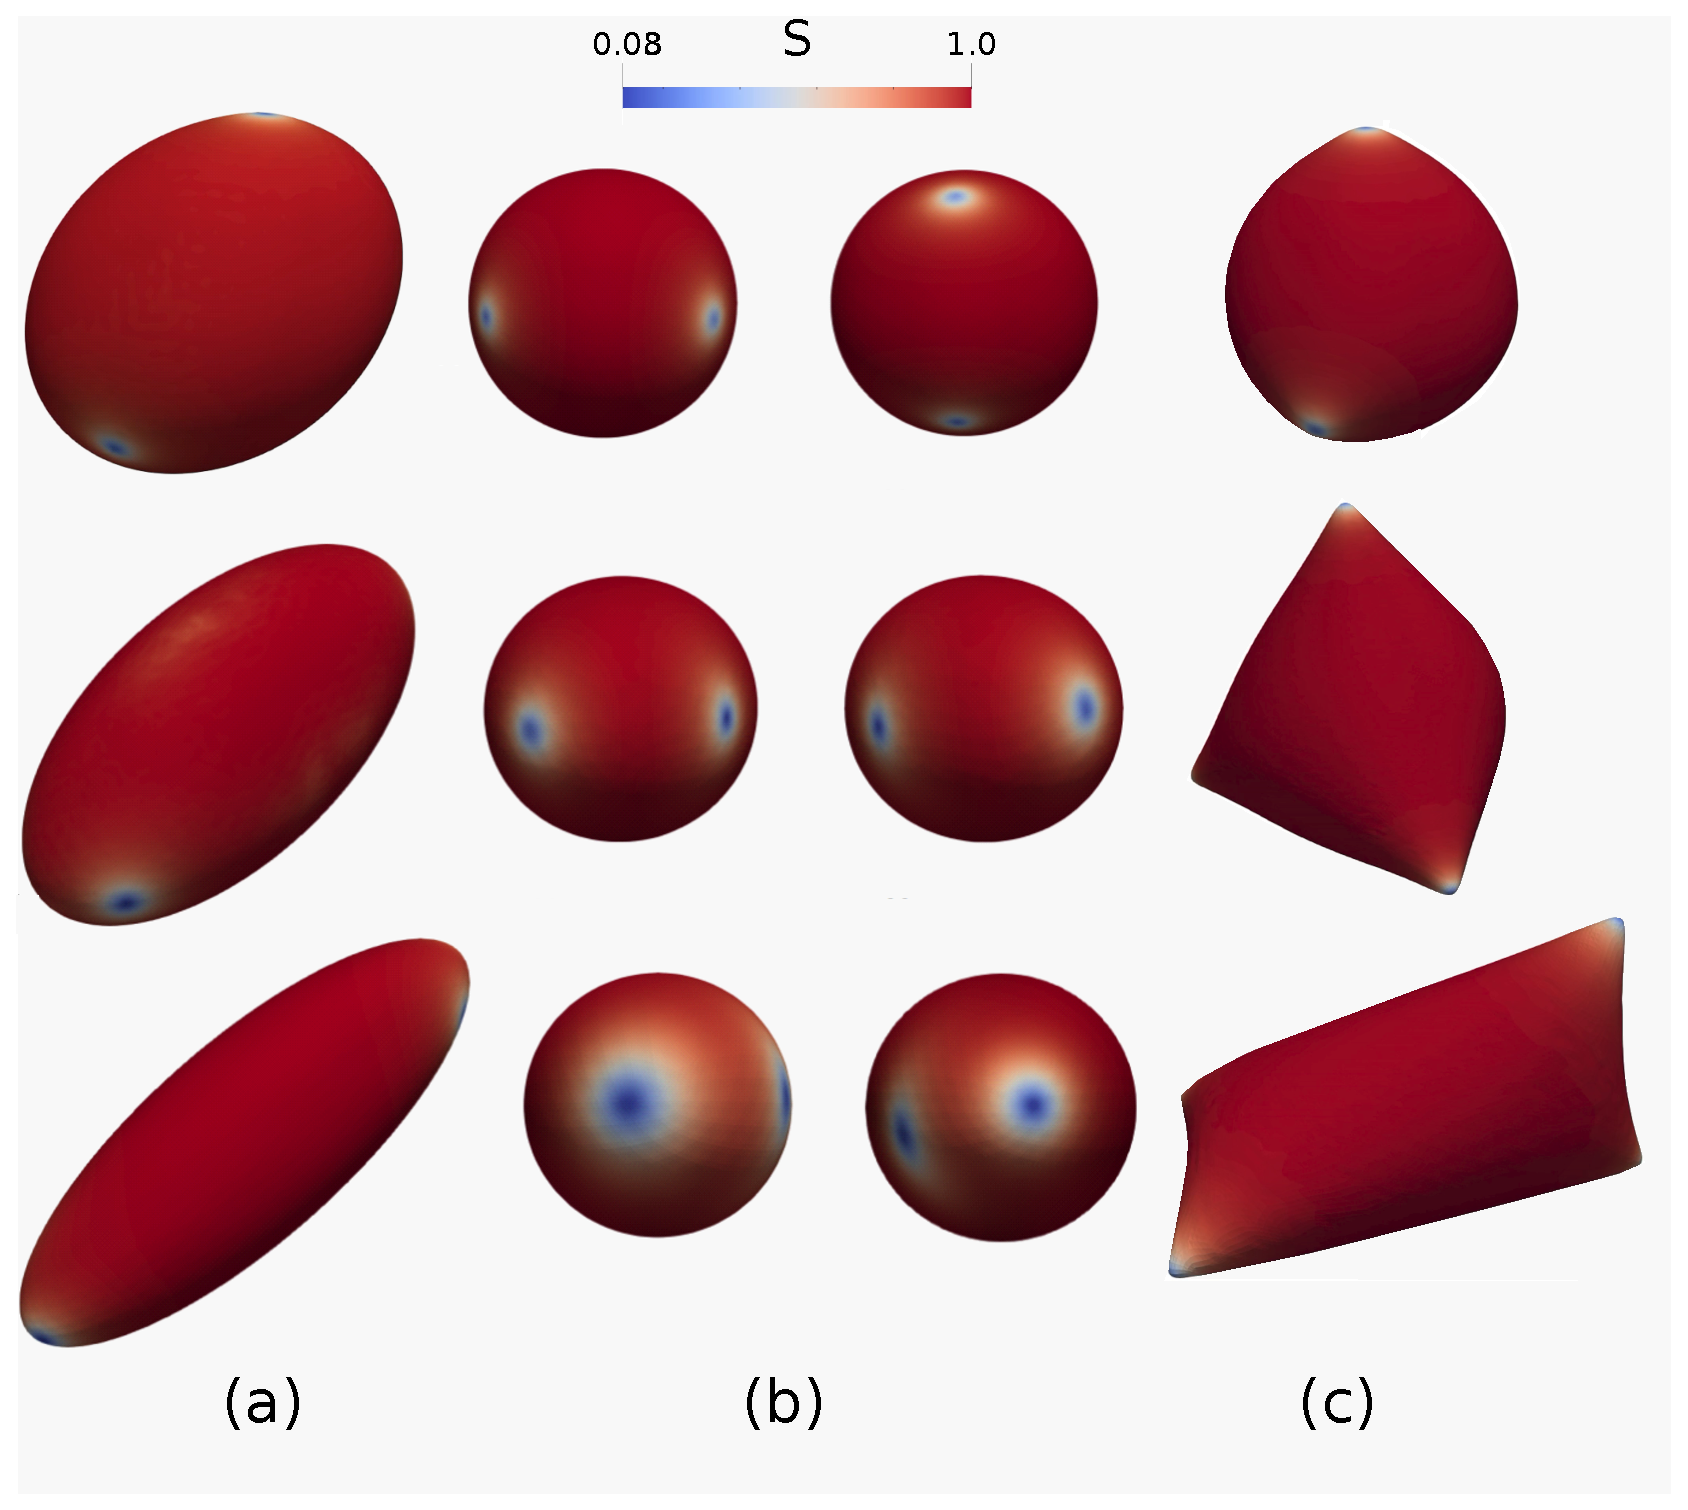
\includegraphics[width=1.\textwidth]{fig9.2.eps}
	\caption{ \textbf{Interplay between shape and nematic field}. (a-b) Different views of the configuration of defects on an initially ellipsoidal surface at short times $\propto \eta_{\rm rot }/|a|$. At these times, shape has not evolved and nematic order is nearly at equilibrium. (a) shows a 3D  perspective whereas (b) show front and back views. (c) Steady state at long times ($\gg \eta/|a|$) once both shape and nematic field have relaxed.  }
	\label{fig9.1}
\end{figure} 
  
 
 \subsection{Dynamics of an active nematic vesicle }
 
 We next examine the interplay between shape and nematic order for an active vesicle, which develops a transient limit cycle with moving defects, shape changes and interfacial flows. Now, nematic and shape relaxations happen at comparable time-scales, $\eta /\eta_{\rm rot} = 1$.

  First, we deflate a spherical passive vesicle by $10\%$ of the original volume, resulting in the formation of an excess membrane due to the inextensibility constraint. We then allow the system to relax, resulting after an interesting transient in a tetrahedral configuration with four $+1/2$ pointy defects, Fig.~\ref{fig9.2}(a-e). We next turn non activity, $\lambda_{\rm aniso}\ne 0$. If activity is small, it only results in a slight change of shape and nematic field. Above a threshold, it leads to a persistent motion of defects and shape changes. During these dynamics, the system  periodically leaves a low-energy tetrahedral state to evolve towards a different symmetry-related tetrahedral state passing through a high-energy state with a planar defect configuration, Fig.~\ref{fig9.2}(f-j) and \href{https://github.com/waleedmirzaPhD/movies_thesis.git}{Movie~$8.5,8.6$}. These results are in agreement with experimental observations on active nematic vesicles \cite{keber2014}.

  
 
 \begin{figure}
 	\centering
 	\hspace*{-0.5cm}\includegraphics[width=1.\textwidth]{fig9.1.pdf}
 	\caption{ \textbf{Effect of activity on the dynamics of defects and shape changes}. (a-e) A passive liquid crystal vesicle is deflated to generate excess area. Afterwards, the nematic field and shape are  allowed to relax, leading to four pointy  $+1/2$ defects in a tetrahedral arrangement. (f-j) The presence of finite activity generates active flows around the defects, which periodically deforms the vesicle oscillating between low-energy tetrahedral states and high-energy planar states.  }
 	\label{fig9.2}
 \end{figure} 


\renewcommand{\thesection}{9.\arabic{section}}
\chapter{Conclusions and future work}	\label{chap_10}
\section{Conclusions}

We have developed a novel theoretical and computational framework to model
and simulate the fully non-linear dynamics of a compressible active nematic gel, both confined to a plane and on a deformable surface. More specifically,
\begin{enumerate}
	\item We have developed a general theoretical framework for active nematic gels based on Onsager's variational formalism, according to which the fully coupled and nonlinear dynamics minimize a functional where free-energy release, dissipation and power input compete. This method provides an unambiguous roadmap to derive complex governing equations from fundamental building blocks and their coupling. For instance, going from a 2D active nematic gel to one on a deformable surface only requires expressing the free-energy, the dissipation potential and the power input covariantly, and then applying the same variational procedure. We have particularized our general framework to active nematic gels which, contrary to common models for incompressible nematic liquid crystals, are not bound by topological nematic constraints since isotropic states can be favorable, and can develop strong density variations, which are essential to understand the active self-organization of the actin cytoskeleton. 
	\item We have developed a computational framework to solve the governing equations of an active nematic gel on 2D fixed domains with arbitrary boundary conditions, on two-dimensional domains with moving boundaries, on axisymmetric deformable  surfaces and on general deformable  surfaces. Onsager's variational formalism naturally lends itself to space and time discretization. For space discretization, we use linear, B-Spline or subdivision finite elements depending on the context. For time discretization, we resort to backward Euler schemes and to a time-incremental version of Onsager's variational method.
	\item We have applied this theoretical and computational framework to understand a variety of biological problems revolving around the active self-organization and dynamics of nematic structures.  In the first part of the thesis focusing on gels confined to a 2D plane, 
	\begin{enumerate}
	\item we have studied the self-assembly of a dense and nematic contractile ring at the edge of a hole or wound in an initially quiescent, isotropic and uniform gel, leading to spontaneous wound healing. 
	\item We have also studied the spontaneous formation and motion of nematic defects and active flows in dense colonies of elongated cells. 
	\item Finally, we have studied the active self-organization of patterns of dense nematic structures starting from quiescent, isotropic and uniform gels. We have mapped how model parameters control the architecture, geometry and dynamics of such patterns. Hence, this study establishes a framework to understand the polymorphism of the actin cytoskeleton. Importantly, this theory provides a mechanism for the self-organization of patterns of dense nematic bundles as observed in a variety of cellular contexts, Figs.~\ref{chap_1_fig_1} and \ref{chap_1_fig_22}. This mechanism imposes requirements on the relation between nematic order and activity in the theory, which we substantiate using out-of-equilibrium discrete network simulations.
	\end{enumerate}
	In the second part of the thesis focusing on active nematic gels on deformable surfaces
	\begin{enumerate}
	\item we have reproduced the self-organization of a dense and nematic cytokinetic ring from either an equatorial over-activity or as a symmetry-breaking spontaneous mode. We have shown that the nematic coupling facilitates complete cell division and accelerates the process. We have also briefly explored the competition between cytokinetic and polarized symmetry-breaking dynamical modes. 
	\item Turning to an inextensible, active and nematic liquid crystal confined to a vesicle, we have examined the interplay between nematic defects and curvature.
	\end{enumerate}
\end{enumerate}

\section{Future work}

This thesis is also a foundation to develop the following research avenues, which are either proposed or actual ongoing research projects.

\subsection*{Dynamics of topological defects in nematic cell monolayers}

  Spindle-shaped cells such as fibroblasts, myoblasts, or some epithelial cells self-organize into domains with high nematic order and $\pm 1/2$ topological defects  \cite{duclos2017, guillamat2020}. These multicellular defects organize well-defined orientational patterns that lead to reproducible flow and force fields generated by active processes in the actomyosin cytoskeleton. Although the interplay between orientational patterns around topological defects and forces has been elucidated for epithelial cell monolayers \cite{balasubramaniam2021}, it remains elusive for mesenchymal tissues, where, mainly due to a lower cell-cell adhesion and apolar cell migration, defect dynamics are notably different. %In particular, we are interested in understanding the mechanical roles of topological defects in these systems.
To understand the mechanisms underlying nematic, flow, and force patterns around possibly motile defects in mesenchymal-like cell monolayers, we plan to combine quantitative observations of in vitro cell cultures and numerical simulations based on an active nematic gel theory. We plan to compare experimentally measured nematic orientation fields, flow fields and monolayer-substrate traction fields around $\pm 1/2$ topological defects along with defect dynamics with theoretical prediction to establish the interplay between active and passive forces in the system. Once the active nematic gel parameters have been identified, we plan to use the model to devise strategies to rationally manipulate cellular active matter around nematic defects.
%This project aims to characterize the mechanisms underlying defect motility in mesenchymal-like cell monolayers by using a combination of in vitro cell culture experiments and numerical simulations. The latter are based on the conception that the defect dynamics result from an interplay between elastic nematic energy, active processes, and dissipative effects, namely viscous flow of cells and friction from the interaction between the cells and the substrate.
%In our experimental setup,  we prepare nematic monolayers of fibroblasts on soft, cell-deformable, elastomeric substrates ($\sim$kPa) coated with nanometric fluorescent tracer beads. We then simultaneously obtain images of the cell monolayers and the fluorescent beads underneath, using brightfield and confocal microscopy, respectively. By computationally analyzing our brightfield images, we can extract the average local orientation,  the position of topological defects and flows, the latter by using Particle Image Velocimetry (PIV). On the other hand, by calculating the displacements of the beads with respect to the relaxed substrate (without cells) we can quantify the traction forces (traction force microscopy, TFM). Altogether, this approach allows us to correlate orientation, velocity, and traction force fields as well as to unveil the velocity and force fields corresponding to $\pm 1/2$ topological defects. 
%\begin{figure}[h!]
%	\includegraphics[width=\textwidth]{Defects_WM.jpg}
%	\caption{Traction force patterns generated by half-integer cellular topological defects. Black vectors correspond to average cellular orientation around negative (left) and positive (right) half-integer defects. White vectors correspond to the corresponding average traction force fields. The color map indicates the radial component of the traction forces.}
%\end{figure}
%Preliminary data reveals that, upon cell confluence, fibroblast monolayers behave as quasi-static active nematic. Very different from jammed epithelial layers \cite{trepat2009}, deprived of any orientational order, dense fibroblast monolayers preserve well-defined and immobile liquid-crystalline-like phases that lead to the organization of robust stress patterns at the position of topological defects, which remain pinned in their formation position. To investigate the link between active and passive forces in this system, we probe the influence of both cell-cell adhesion and cellular contractility on defect motility. Both by decreasing inter-cellular contacts (viscosity and friction), and contractility (active stress) we observe a fast displacement of defects that we relate with an elastic relaxation of the cellular sheet. These experiments reveal that mesenchymal cell monolayers behave as an active viscoelastic active sheets with accumulated stresses at the positions of topological defects that source from multi-cellular collective effects. 
%With our model, we first aim to establish a protocol to estimate material parameters of the active nematic viscous model by solving a least squares optimization problem using the experimental data points. Next, we aim to validate the trends of these active topological defects by characterizing velocity, nematic, and traction fields against numerical solutions of the proposed active nematic viscous model and furthermore using the numerical solution to investigate the underlying mechanisms governing defects dynamics.

\subsection*{Active self-organization of dense nematic bundles beyond the onset}

		We have identified in Chapter~\ref{chap_4} mechanisms for the active self-organization of dense nematic bundles beyond the linear instability.  However, to describe the maturation of these emergent nematic structures in cells, e.g.~leading to stress fibers, our theory needs to be enriched in various ways. We briefly discuss next four possible avenues. First, the active gel presented here stores elastic nematic energy but not elastic strain energy. However, mature stress fibers are viscoelastic \cite{KUMAR20063762,doi:10.1091/mbc.E18-02-0106}, particularly on stiff substrates \cite{gupta2015}. This effect can be included in an active gel formalism \cite{Prost:2015aa} and should affect the rapid reorganization of fibers. Second, mature nematic bundles can be highly contractile along the nematic direction due to the action of myosin motors, but in our model, active tension needs to be larger perpendicular to this direction to assemble such structures in the first place. This seeming contradiction can be addressed by switching the sign of tension anisotropy parameter $\kappa$ from negative to positive as density, order and/or an additional field accounting for a maturation species increase. Third, the structure, dynamics and function of stress fibers crucially depends on adhesion complexes with the extracellular matrix, including focal adhesions at their ends but also distributed adhesion along fiber length \cite{10.1242/jcs.042986}. The interplay between emergent cytoskeletal and adhesive patterns \cite{doi:10.1098/rsif.2007.1182} may explain the establishment of the stress-fiber/focal-adhesion architecture of adherent cells, known to be strongly influenced by matrix rigidity \cite{Zemel:2010aa,gupta2015} and adhesive size \cite{jalal2019}.

\subsection*{Active self-organization of dense nematic bundles in cell-like geometries}

The formation of patterns of nematic bundles strongly depends on cellular-scale shape, heterogeneity or boundary conditions. Understanding such circular, chiral, radial or nematic bundle patterns requires considering a cell-scale model beyond the periodic domain considered in Chapter~\ref{chap_4}. Clear examples of cellular heterogeneity or boundary conditions affecting the actin cytoskeleton include polymerization at the leading edge, steric hindrance of the nucleus in adherent cells or during cellularization, cell polarization during directed migration or more generally gradients of regulators of the actomyosin cytoskeleton  \cite{dudin2019,tojkander2015}. These conditions control the assembly, maturity, and coexistence of various families of actin nematic bundles such as radial and transverse stress fibers \cite{tojkander2015}. Inspired by the remarkably reproducible patterns of stress fibers in cells confined to adhesive patterns, Fig.~\ref{chap_1_fig_22}, we aim to study the self-organization of actin nematic bundles in a circular domain mimicking an adherent cell. Changing the shape of the domain is straightforward with our finite element computational approach. We plan to extend the model proposed in Chapter~\ref{chap_2} to include three distinct density fields for cross-linkers $\rho_{\rm cross}$, myosin-II  $\rho_{\rm myo}$ and actin filaments $\rho_{\rm actin}$ as these fields do not necessarily coincide \cite{lehtimaki2021}. Moreover, myosin-II  and bundling cross-linkers exert in principle active stresses of different nature, either along or perpendicular to the nematic direction: $ \rho_{\rm myo} \lambda_{\rm myo} S n_a n_b$ and  $\rho_{\rm cross} \lambda_{\rm cross} S m_a m_b$.

\begin{figure}[H]
	\centering
	\includegraphics[width=1\textwidth]{chap_10_fig.pdf}
	\caption{\textbf{Self-organization of actin bundles in a cell-like geometry and boundary conditions}. (I.a) Domain and boundary conditions leading to the self-organization of transverse stress fibers. (I.b) Snapshots illustrating the development of a self-organized pulsating dynamical state in which transverse bundles nucleate near the cell periphery, move inwards, and disassemble near the nucleus. (II.a) Domain and boundary conditions leading to the self-organization of radial stress fibers. (II.b) Snapshots showing the self-organization radial nematic bundles from the leading edge and elongating to reach the nucleus.}
	\label{fig::1_chap10}
\end{figure}

Preliminary results with the extended model are illustrated in Fig.~\ref{fig::1_chap10} for different boundary conditions. We first considered a radial inwards flow in the outer boundary and zero normal flow at the inner boundary, modeling actin polymerization at the leading edge and the steric hinderance of the nucleus, Fig.~\ref{fig::1_chap10}(I). Starting from a uniform and isotropic gel, the system self-organizes transverse dense nematic bundles as follows: (I.b.i) The actin polymerized at the leading edge flows radially toward the center of the cell. As the actin network flows, the substrate exerts an opposing friction force proportional to the polymerization velocity. This impediment to the flow results in the densification of the gel at a distance similar to the hydrodynamic length $\ell_0$ from the leading edge. As the flow slows down due to friction, the actin network experience a local compression favoring network alignment tangential to the leading edge. (I.b.ii) The active alignment controlled by $\lambda_\odot$ and triggered by the incipient densification and ordering further increases alignment and condensation of the dense nematic arch. (I.b.iii-v) The arch being contractile, it moves inwards due to a Laplace-like force. As it moves inwards, a new arch is nucleated in the cell periphery by the same mechanism. (I.b.vi) As soon as an arch reaches the proximity of the nucleus, in agreement with observations of myosin-II depletion, we drop activity leading to arch disassembly. This sequence of events leads to a  pulsatile flow where a train of contractile arches self-organize close to the leading edge, flow radially, and disintegrate close to the cell nucleus,  \href{https://github.com/waleedmirzaPhD/movies_thesis.git}{Movie~9.1}.



Next, along with the velocity boundary conditions, we prescribed homeotropic boundary conditions for the nematic field consistent with the idea that, as the polar lamellipodium moves backward and loses polarity, it retains some nematic orientational order. Furthermore, we imposed and increased $\rho_{\rm cross}$ at the leading edge and an increased $\rho_{\rm myo}$ close to the nucleus \cite{tee2015, lehtimaki2021}, Fig.~\ref{fig::1_chap10}(II). As shown in the Fig.~\ref{fig::1_chap10} and in  \href{https://github.com/waleedmirzaPhD/movies_thesis.git}{Movie~9.2}, these conditions break the polar symmetry and lead to self-organized regularly spaced radial bundles with high nematic order and density at the leading edge. Once nucleated, they elongate as they are advected towards the nucleus due to the inwards polymerization velocity boundary condition.

These preliminary calculations suggest that the complex and dynamical stress fiber patterns in adherent may result from the modulation by cell geometry, heterogeneity, and boundary conditions of the intrinsic ability of the actin cytoskeleton to self-organize dense nematic bundles.

\subsection*{Systematic understanding of the interplay between shape and self-organized nematic structures}

Chapter~\ref{chap_8} has illustrated the tight coupling between cortical flows, density accumulation, nematic ordering and cell shape during cell morphogenesis. Towards a comprehensive mapping between active gel parameters and distinct self-organized dynamical modes involving dense nematic structures, we plan to perform linear stability analysis of the proposed active nematic gel on a deformable surface. Such a study, along with  nonlinear simulations avoiding the assumption of axisymmetry, may elucidate the conditions leading to cellular oscillations \cite{gorfinkiel2016,maitre2015}, to robust division \cite{yoshizaki2003}, to incomplete furrowing and cell elongation \cite{Dong}, or to polarized motility modes \cite{Ruprecht:2015aa}.
 
Likewise, on liquid crystal active nematic surfaces, defects are known to generate out-of-plane forces and hence trigger shape changes. This mechanism serves as a precursor of morphogenesis. For instance, during Hydra development, the locations of the early  mouth, foot, and tentacles correlate with $+1$ vortex-like defects \cite{maroudas2021}. Similar defect-induced shape transformations have been observed in active nematic vesicles \cite{keber2014} or in  myoblast cell cultures \cite{guillamat2020}. These and other defect-driven active morphogenetic events can be understood with the theoretical and computational models proposed in Chapters \ref{chap_7} and \ref{chap_9}.



%
%
\begin{appendices}
	\renewcommand{\thesection}{A.\arabic{section}}
	\chapter{Active self-organization of nematic architecture on a flat surface }   \label{appendix_1}
		\section{Onsager inequality} \label{inequality}
We show that the active nematic system evolves in a way that the proposed dissipation potential is always positive, that is, 
\begin{align}
	d &  = \eta \big( d_{ab} d_{ab}   + (\text{tr}d)^2  \big) + \frac{\eta_{\text{rot}}}{2} \widehat{q}_{ab} \widehat{q}_{ab}  + \beta d_{ab}^{\rm dev}\widehat{q}_{ab} + \frac{\gamma}{2} v_a v_a \geq 0  \\ & = 
	2\eta \big( d_{11}^2 + d_{12}^2 + d_{22}^2  + d_{11}d_{22} \big) + \eta_{\text{rot}} \big( \widehat{q}_{1}^{\, \, 2} + \widehat{q}_{2}^{\, \, 2}  \big) + \beta \big(d_{11}\widehat{q}_{1} - d_{22}\widehat{q}_{1} + \nonumber  2d_{12}\widehat{q}_{2}\big)  \\ &  +  \nonumber  \frac{\gamma}{2} \big(v_1^{\,2} + v_2^{\,2}\big) \geq 0 \nonumber.
\end{align}
In form of matrix, the component-wise dissipation potential is re-written as $	z_{a} M_{ab} z_b\geq 0,$
where
\begin{align}
	\bm{z} = \begin{pmatrix}
		d_{11}\\ 
		d_{22}\\ 
		d_{12}\\ 
		q_{1}\\ 
		q_{2}\\ 
		v_1\\ 
		v_2\\ 
	\end{pmatrix}, \quad  \bm{M} = \begin{pmatrix}
		2\eta& \eta &0  &\beta/2  &0  &0  &0   \\ 
		\eta& 2\eta &0  &-\beta/2  &0  &0  &0   \\ 
		0&  0&  2\eta&  0& \beta &0  &0   \\ 
		\beta/2& -\beta/2 &0  &\eta_{\rm rot}  &0  &0  &0   \\ 
		0&  0 &\beta  & 0 & \eta_{\rm rot} &0  &0   \\ 
		0& 0 & 0 & 0 & 0 & \gamma/2 & 0  \\ 
		0& 0 & 0 & 0 & 0 & 0 & \gamma/2
	\end{pmatrix}.
\end{align}
According to the Sylvester's criterion \cite{doi:10.1080/00029890.1991.11995702}, for $\bm{M}$ to be a positive definite tensor it should be symmetric with positive leading principal minors. Upon inspecting the principle minors of matrix $\bm{M}$, we arrive to the following condition on the model parameters that ensures that $ d  \geq 0$
\begin{equation}
	2\eta \eta_{\rm rot} - \beta^2 \geq 0.
\end{equation}
\section{Equivalence between weak and strong forms} \label{equivalence}

In this section, we establish an equivalence between strong and weak balance of force conjugate to velocities. For doing so, we have to prove that
\begin{equation}
	\label{eq:weak_v_disc_app}
	\begin{aligned}
		&\underset{ A}{\int} \bigg \{-\frac{ f}{\rho} \nabla_d \left(\rho u_d\right)  + \frac{\partial ( d+ p)}{\partial \widehat{q}_{ab}}  \left[\nabla_c q_{ab} u_c +\frac{1}{2}\left(q_{ac} \epsilon_{cb}-\epsilon_{ac}q_{cb}\right) \epsilon_{de}\nabla_e u_d\right] \bigg \}\rho dA \\
		&+  \int_{\partial_{N_{\bm{t}}} A} \bigg\{f\rho N_c u_c - L_{ab} \left[\nabla_c q_{ab} u_c +\frac{1}{2}\left(q_{ac} \epsilon_{cb}-\epsilon_{ac}q_{cb}\right) \epsilon_{de}\nabla_e u_d\right] \bigg\}dl,
	\end{aligned}
\end{equation}
is equal to 
\begin{equation}
	\label{eq:weak_v_app}
	\begin{aligned}
		\underset{A}{\int} \sigma^e_{ab}\nabla_b u_a dA + \int_{\partial_{N_{\bm{t}}} A} ( m_c N_c)\epsilon_{ab} \nabla_b v_a dl,
	\end{aligned}
\end{equation}
where $\bm{\sigma}^e$ is the elastic part of the total stress, i.e, 
\begin{equation}
	\sigma_{ab}^e = -\frac{1}{2} \bigg[\left(\nabla\cdot\bm{m}\right)\epsilon_{ab} - \rho \left(\frac{\partial  f}{\partial \nabla_b q_{dc}} \nabla_a q_{dc}+ \frac{\partial  f}{\partial \nabla_a q_{dc}} \nabla_b q_{dc}\right) \bigg].
\end{equation}
We first integrate the first term in the second line of Eq.~\eqref{eq:weak_v_disc_app}, to get
\begin{equation}
	\label{eq:weak_v_disc_app2}
	\begin{aligned}
		&\underset{ A}{\int} \bigg \{  u_d \nabla_d f + \frac{\partial ( d+ p)}{\partial \widehat{q}_{ab}} \left[\nabla_c q_{ab} u_c +\frac{1}{2}\left(q_{ac} \epsilon_{cb}-\epsilon_{ac}q_{cb}\right) \epsilon_{de}\nabla_e u_d\right] \bigg \} \rho dA \\
		&+  \int_{\partial_{N_{\bm{t}}} A} \bigg\{ -L_{ab} \left[\nabla_c q_{ab} u_c +\frac{1}{2}\left(q_{ac} \epsilon_{cb}-\epsilon_{ac}q_{cb}\right) \epsilon_{de}\nabla_e u_d\right]  \bigg\}dl.
	\end{aligned}
\end{equation}
We now note that from the first expression in Eq.~\eqref{eq:balance_q}
\begin{equation}
	\frac{\partial ( d+ p)}{\partial \widehat{q}_{ab}} =  \frac{1}{\rho}\nabla_c \left(\rho \frac{\partial f}{\partial \nabla_c q_{ab}} \right) - \frac{\partial f}{\partial q_{ab}}, 
\end{equation}
and thus
\begin{equation}
	\label{eq:weak_v_disc_app3}
	\begin{aligned}
		&\underset{ A}{\int} \bigg \{  u_d \nabla_d f + \left[ \frac{1}{\rho}\nabla_c \left(\rho \frac{\partial f}{\partial \nabla_c q_{ab}}\right) - \frac{\partial f}{\partial q_{ab}} \right] \left[\nabla_c q_{ab} u_c +\frac{1}{2}\left(q_{ac} \epsilon_{cb}-\epsilon_{ac}q_{cb}\right) \epsilon_{de}\nabla_e u_d\right] \bigg \} \rho dA \\
		&+  \int_{\partial_{N_{\bm{t}}} A} \bigg\{  -L_{ab} \left[\nabla_c q_{ab} u_c +\frac{1}{2}\left(q_{ac} \epsilon_{cb}-\epsilon_{ac}q_{cb}\right) \epsilon_{de}\nabla_e u_d\right]  \bigg\}dl.
	\end{aligned}
\end{equation}
We integrate by parts the first term in the first square brackets 
\begin{equation}
	\label{eq:weak_v_disc_app4}
	\begin{aligned}
		&\underset{ A}{\int} \bigg \{  u_d \nabla_d f - \frac{\partial f}{\partial q_{ab}} \left[\nabla_c q_{ab} u_c +\frac{1}{2}\left(q_{ac} \epsilon_{cb}-\epsilon_{ac}q_{cb}\right) \epsilon_{de}\nabla_e u_d\right] \\
		&- \left( \frac{\partial f}{\partial \nabla_c q_{ab}}\right) \nabla_c \left[\nabla_d q_{ab} u_d +\frac{1}{2}\left(q_{ad} \epsilon_{db}-\epsilon_{ad}q_{db}\right) \epsilon_{ef}\nabla_f u_e\right] \bigg \} \rho dA \\
		&+  \int_{\partial_{N_{\bm{t}}} A} \bigg\{ \left[\left(\rho \frac{\partial f}{\partial \nabla_c q_{ab}}\right) N_c-L_{ab} \right] \left[\nabla_c q_{ab} u_c +\frac{1}{2}\left(q_{ac} \epsilon_{cb}-\epsilon_{ac}q_{cb}\right) \epsilon_{de}\nabla_e u_d\right]   \bigg\}dl,
	\end{aligned}
\end{equation}
but the first term in the boundary cancels because of the second line of Eq.~\eqref{eq:balance_q}, so we have
\begin{equation}
	\begin{aligned}
		&\underset{ A}{\int} \bigg \{  u_d \nabla_d f - \frac{\partial f}{\partial q_{ab}} \left[\nabla_c q_{ab} u_c +\frac{1}{2}\left(q_{ac} \epsilon_{cb}-\epsilon_{ac}q_{cb}\right) \epsilon_{de}\nabla_e u_d\right] \\
		&- \left( \frac{\partial f}{\partial \nabla_c q_{ab}}\right) \nabla_c \bigg[\nabla_d q_{ab} u_d +\frac{1}{2}\left(q_{ad} \epsilon_{db}-\epsilon_{ad}q_{db}\right) \epsilon_{ef}\nabla_f u_e\bigg] \bigg \} \rho dA.
	\end{aligned}
\end{equation}
Furthermore, we now note that 
\begin{equation}
	\nabla_d f = \frac{\partial f}{\partial q_{ab}}\nabla_d q_{ab} + \frac{\partial f}{\partial \nabla_c q_{ab}} \nabla_c \nabla_d q_{ab}.
\end{equation}
After plugging the expression above in Eq.~(\ref{eq:weak_v_disc_app4}), we simplify the expression above to 
\begin{equation}
	\label{eq:weak_v_disc_app5}
	\begin{aligned}
		&\underset{ A}{\int} \bigg \{   - \frac{\partial f}{\partial q_{ab}}  \bigg[\frac{1}{2}\left(q_{ac} \epsilon_{cb}-\epsilon_{ac}q_{cb}\right) \epsilon_{de}\nabla_e u_d\bigg] \\
		&-  \frac{\partial f}{\partial \nabla_c q_{ab}} \nabla_d q_{ab} \nabla_c u_d + \frac{1}{2} \frac{\partial f}{\partial \nabla_c q_{ab}} \nabla_c\bigg[\left(q_{ad} \epsilon_{db}-\epsilon_{ad}q_{db}\right) \epsilon_{ef}\nabla_f u_e\bigg] \bigg \} \rho dA .
	\end{aligned}
\end{equation}
Due to the symmetry to $q_{ab}$ the first term above is rendered zero and the expression is simplified to
\begin{equation}
	\label{eq:weak_v_disc_app6}
	\begin{aligned}
		&\underset{ A}{\int} \bigg \{ -\frac{\partial f}{\partial \nabla_c q_{ab}}  \nabla_d q_{ab} \nabla_c u_d +\frac{1}{2} \frac{\partial f}{\partial \nabla_c q_{ab}} \nabla_c\bigg[\left(q_{ad} \epsilon_{db}-\epsilon_{ad}q_{db}\right) \epsilon_{ef}\nabla_f u_e\bigg] \bigg \} \rho dA ,
	\end{aligned}
\end{equation}
We symmetrize the first term above as
\begin{equation}
	\label{eq:weak_v_disc_app7}
	\begin{aligned}
		&\underset{ A}{\int} \frac{1}{2}\bigg \{  -\left(\frac{\partial f}{\partial \nabla_c q_{ab}}  \nabla_d q_{ab} + \frac{\partial f}{\partial \nabla_d q_{ab}}  \nabla_c q_{ab}  \right)\nabla_c u_d + \frac{\partial f}{\partial \nabla_c q_{ab}} \nabla_c\bigg[\left(q_{ad} \epsilon_{db}-\epsilon_{ad}q_{db}\right) \epsilon_{ef}\nabla_f u_e\bigg] \bigg \} \rho dA ,
	\end{aligned}
\end{equation}
Now we apply integration by parts to term in the square bracket above and apply the divergence theorem
\begin{equation}
	\label{eq:weak_v_disc_app8}
	\begin{aligned}
		&\underset{ A}{\int} \frac{1}{2}\bigg \{  -\left(\frac{\partial f}{\partial \nabla_c q_{ab}}  \nabla_d q_{ab} + \frac{\partial f}{\partial \nabla_d q_{ab}}  \nabla_c q_{ab}  \right)\nabla_c u_d - \nabla_c \left( \frac{\partial f}{\partial \nabla_c q_{ab}}\right)  \left(q_{ad} \epsilon_{db}-\epsilon_{ad}q_{db}\right) \epsilon_{ef}\nabla_f u_e \bigg \} \rho dA   \\
		& + \underset{ \partial A}{\int} \frac{1}{2}\frac{\partial f}{\partial \nabla_c q_{ab}} \left(q_{ad} \epsilon_{db}-\epsilon_{ad}q_{db} \right) \epsilon_{ef} N_c \nabla_f u_e \rho d l .
	\end{aligned}
\end{equation}
Finally, by taking into account Eqs.~\eqref{eq:sym_stress}, \eqref{eq:moment}, and \eqref{eq:balance_angular_momentum}, one can write the expression above as in Eq.~\eqref{eq:weak_v_app}.
\section{Grid convergence analysis} \label{appendix_grid}
We validate our numerical methods for the spatial discretization by solving the proposed model for various mesh sizes. For this purpose, we use a test case of a passive nematic system in circular confinements, see Fig.~\ref{sec_1_chap_3_fig_2}, for $\ell_p/\ell_0=0.04$. We use the normalized error of free-energy at steady state 
\begin{align}	
	e^x = \frac{|F^h -F^*|}{|F^*|} , 
\end{align}
where $F^h$ is the free-energy of a finite element solution with mesh-size $h$ and $F^*$ is that of an overkill solution computed with a very fine mesh of $n_e = 695,296$ triangular elements. We plot the energy error norm for decreasing mesh sizes, Fig.~\ref{grid}(a). The results show the expected optimal convergence (slope of 2 in a log-log scale) for linear elements. 


Next for the same numerical experiment, we validate the temporal convergence by gradually decreasing the
time step $\Delta t$ used to reach a fixed time point $t|a|/\eta_{\rm rot}=1$. We calculate the relative  the error norm  as
\begin{align}	
	e^t = \frac{|F^{\Delta t} -F^{t,*}|}{|F^{t,*}|} , 
\end{align}
where $F^{\Delta t}$ is the free-energy obtained with time-step $\Delta t$  at $t|a|/\eta_{\rm rot}=1$ and   $F^{t,*}$ is the free-energy with a very small time-step $\Delta t^* = 10^{-5}$. As expected, Fig.~\ref{grid}(b), the free-energy converges with a slope $\sim \Delta t$.
\begin{figure}[tb]
	\centering
	\includegraphics[width=\textwidth]{append.pdf}
	\caption{\label{grid} Validation of convergence behaviour of the numerical model. (a) Convergence of the spatial discretisation. The relative free-energy error $e^x$  shows a convergence rate $\sim h^{2}$. (b) Convergence of the temporal discretisation. The relative free-energy error  $e^{\Delta t}$  shows a convergence rate $\sim \Delta t$.}
\end{figure}

	\section{\label{sec:level1}1D reduced model} \label{appendix_1_sec_4}

To perform the linear stability analysis, we reduce the theoretical model to 1D  by considering the flow velocity $v(x,t)$  and the density field as $\rho(x,t)$ along the $x-$axis. The nematic order tensor is defined as $q_{ij} = S(n_i n_j - \delta_{ij}/2)$, where $\bm{n}$ is the local average filament orientation and $S$ is the local degree of alignment. Since it is traceless and symmetric, in general it can be represented by 2 independent degrees of freedom, $q_{11}=-q_{22}=q_1$ and $q_{12}=q_{21}=q_2$. In the 1D model we assume that $\bm{n}$ is either along or perpendicular to $x$, and hence $q_{12}=q_{21}=0$. We are thus left with one independent degree of freedom $q_{11}=-q_{22}=q$. Positive (negative) $q$ represents alignment along (perpendicular to) the $x-$axis. The Jaumann derivative of the nematic order parameter reduces in 1D to
\begin{equation}
	\hat{q}=\frac{\partial q}{\partial t} + v \frac{\partial q}{\partial x}.
\end{equation}
Particularizing the general equations given in the Chapter~\ref{chap_4} and systematically derived in Chapter~\ref{chap_2}, we present next the 1D governing equations pertinent to the linear stability analysis. Mass conservation reads
\begin{equation} \label{eq_1D_thick}
	\frac{\partial \rho }{\partial t}  + \frac{\partial}{\partial x} \left( \rho v \right)   -  D \frac{\partial^2 \rho}{\partial x^2}  + k_d (\rho-\rho_0)=0,
\end{equation}
balance of linear momentum of the active gel reduces to
\begin{equation} \label{eq_1D_force_balance}
	\rho \gamma   v =    \frac{\partial \sigma}{\partial x}   \, ,
\end{equation}
where stress along $x$, $\sigma$, is given by
\begin{equation} \label{eq_1D_stress}
	\sigma = \rho \left[  4 \eta \frac{\partial v}{\partial x}+ \beta  \hat{q}  +  \lambda \left( 1+\kappa q \right) - 2L \left( \frac{\partial q}{\partial x}\right)^2  \right].
\end{equation}
The evolution of nematic order $q$ is governed in the 1D setting by
\begin{equation} \label{eq_1D_torque}
	\eta_{\text{rot}} \hat{q} + \frac{\beta}{2} \frac{\partial v}{\partial x}+\left(2a - \rho \lambda_{\odot}+ 4bq^2\right)q - L \frac{\partial^2 \, q}{\partial x^2} - \frac{L}{\rho} \frac{\partial \, q}{\partial x} \frac{\partial \, \rho}{\partial x} = 0 \, .
\end{equation}
For $c_0=2a-\rho_0 \lambda_{\odot} \ge 0$, the uniform steady state of the system is given by $\rho(x,t) = \rho_0$, $v(x,t)=0$ and $q(x,t) = 0$. For $c_0<0$, the uniform steady state has spontaneous alignment given by  $q(x,t) = q_0 = \pm \frac{1}{2} \sqrt{-c_0/b}$. Finally, we note that, for the dissipation to be positive, the material parameters need to satisfy Onsager's inequality $4\eta \eta_{\rm rot} - \beta^2 \ge 0$ in the reduced one-dimensional model and  $2\eta \eta_{\rm rot} - \beta^2 \ge 0$ in the two-dimensional model, see Section~\ref{inequality}.

\pagebreak
\section{\label{sec:level2}Non-dimensionalization}  \label{appendix_1_sec_5}


We present next a non-dimensionalization of the governing Eqs.~(\ref{eq_1D_thick}$-$\ref{eq_1D_torque}). We choose the hydrodynamical length-scale $\ell_s=\sqrt{\eta / \gamma}$, above (below) which friction (viscosity) is the dominant dissipative mechanism in the active gel, and the time-scale of diffusion over this length-scale, $t_0 = \ell_s^2  /  D = \eta /(\gamma D)$. Using these characteristic scales, we non-dimensionalize space and time as $\bar{x} = x/\ell_s$ and $\bar{t}=t/t_0$. We chose $\rho_0$ as a reference density and thus $ \bar{\rho} =  \rho  / \rho_0$. Here and elsewhere, overbar denotes non-dimensional quantities.

The dimensionless balance of mass reads
\begin{equation}{}
	\label{eq_dimensionless_density}
	\frac{\partial \bar{\rho} }{\partial \bar{t}} + \bar{v}\frac{\partial \bar{\rho}}{\partial \bar{x}} +  \bar{\rho} \frac{\partial \bar{v}}{\partial \bar{x}} -  \frac{\partial^2 \bar{\rho}}{\partial \bar{x}^2}  + \bar{k}_d (\bar{\rho}-1)=0,
\end{equation}
where $\bar{k}_d= k_d t_0$. The dimensionless balance of linear momentum reads
\begin{equation} \label{eq_dimensionless_force}
	\bar{\rho} \bar{v} =  \frac{\partial \bar{\sigma}}{\partial \bar{x}}  \, ,
\end{equation}
where $\bar{\sigma} = \sigma / \sigma_0$ and the characteristic stress is given by $\sigma_0= \rho_0  \gamma D$. The non-dimensional constitutive relation for the stress is
\begin{align} \label{eq_dimensionless_stress}
	\bar{\sigma} = \bar{\rho} \left[   4 \frac{\partial \bar{v}}{\partial \bar{x}}+ \bar{\beta}  \bar{\hat{q}} +  \bar{\lambda} \left( 1+\kappa q \right) - 2\bar{L}  \left( \frac{\partial q}{\partial \bar{x}}\right)^2      \right],
\end{align}
where $\bar{L} = L /(\gamma D \ell_s^2) $, $\bar{\beta} = \beta / \eta$,  and $\bar{\lambda} = \lambda/(\gamma D)$. We note that $\kappa = \lambda_{\rm aniso}/\lambda$ and $q$ are already nondimensional.  Finally, the dimensionless equation of generalized force conjugate to nematic order is given by
\begin{equation}\label{eq_dimensionless_torque}
	\bar{\eta}_{\text{rot}} \bar{\hat{q}} + \frac{\bar{\beta}}{2} \frac{\partial \bar{v}}{\partial \bar{x}}+\left(2\bar{a} - \bar{\rho} \bar{\lambda}_{\odot} +4\bar{b}q^2\right)q - \bar{L} \frac{\partial^2 \, q}{\partial \bar{x}^2}  - \frac{\bar{L}}{\bar{\rho}} \frac{\partial \, q}{\partial \bar{x}} \frac{\partial \, \bar{\rho}}{\partial \bar{x}} = 0 \, .
\end{equation}
where $\bar{\eta}_{\text{rot}} =  \eta_{\text{rot}}/ \eta $,  $\bar{a} =  a\, / \left(\gamma D\right)$, $\bar{b} =  b\, / \left(\gamma D\right) $ and  $\bar{\lambda}_{\odot}=\lambda_{\odot} \,  \rho_0 / ( \gamma D)$.   Inspection of the Eq.~(\ref{eq_dimensionless_torque}) reveals the characteristic nematic length-scale $\ell_q^2={L/ \left | 2a-\lambda_{\odot}\rho_0  \right | }$  and the nematic relaxation time-scale  $t_q = (\ell_q^2 \, \eta_{\rm rot})/L = \eta_{\rm rot}/ \left | 2a-\lambda_{\odot}\rho  \right |$.



\pagebreak
\section{Linear stability analysis} \label{appendix_1_sec_6}

We perform next the linear stability analysis on the 1D model given by the dimensionless Eqs.~(\ref{eq_dimensionless_density}$-$\ref{eq_dimensionless_torque}). For the sake of simplicity of notation, we omit overbars for the dimensionless quantities. We assess the stability of the homogeneous state given by $v(x,t)=0$, $q(x,t) = q_0$ and  $\rho(x,t) = \rho_0$ by examining the fate of infinitesimal perturbations $v \left(x,t\right)=\delta  v \left(x,t\right)$,  $ \, q \left(x,t\right) =q_0 + \delta q \left(x,t\right) $ and $\rho \left(x,t\right)=\rho_0 + \delta \rho \left(x,t\right)$, where  $\left\vert \delta  v \right \vert  \sim \left \vert \delta q \right \vert \sim \left \vert \delta \rho \right \vert \ll1 $. The control parameter in our stability analysis is the activity parameter $\lambda$.

Inserting the infinitesimally perturbed homogeneous states into the governing Eqs.~(\ref{eq_dimensionless_density}$-$\ref{eq_dimensionless_torque}) and ignoring terms that are quadratic in perturbations, the resulting balance of linear momentum equation is
\begin{equation} \label{eq_linearized_force}
	\delta v =  4 \, \frac{\partial^2 \, \delta v}{\partial x^2} + \beta  \frac{\partial^2\, \delta {q}}{\partial t \partial x} + \lambda(1 + \kappa q_0 )   \,\frac{\partial \delta \rho}{\partial x}
	+ \lambda \,  \kappa  \frac{\partial \delta q}{\partial x}.
\end{equation}
The linearized form of Eq.~(\ref{eq_dimensionless_torque}) is
\begin{equation} \label{eq_linearized_torque_density}
	\eta_{\text{rot}}  \frac{\partial \delta q}{\partial t} + \frac{\beta}{2} \frac{\partial \delta v}{\partial x} + \underbrace{\left[2a-\rho_0\lambda_\odot + 4bq_0^2 + 8 b q_0^2\right]}_{G} \delta q -  \lambda_{\odot} q_0 \, \delta \rho  - L \frac{\partial^2 \, \delta  q}{\partial x^2}   = 0.
\end{equation}
If $c_0 = 2a - \rho_0 \lambda_\odot>0$, then $q_0 = 0$ and $G = c_0$. If $c_0 = 2a - \rho_0 \lambda_\odot<0$, then $q_0^2 = -c_0/(4b)$ and $G=8 b q_0^2$. The linearized balance of mass reads
\begin{equation} \label{eq_linearized_mass}
	\frac{\partial  \delta \rho }{\partial t} + \frac{\partial \delta v}{\partial x} -  \frac{\partial^2 \delta \rho}{\partial x^2}  + k_d \delta \rho=0.
\end{equation}
We decompose perturbations into a sum of Fourier terms, i.e., $\delta v = v' \,  e^{\alpha t + \mi x\nu}$, $\delta \rho = \rho' \, e^{\alpha t + \mi x\nu}$ and $\delta q = q' \,  e^{\alpha t + \mi x\nu}$, where $v'$, $q'$ and $\rho'$ are the amplitudes of the perturbations, $\alpha$ is the growth rate and $\nu$ is the  wavenumber.

Substituting the Fourier representation in Eq.~(\ref{eq_linearized_force}), we obtain
\begin{equation}
	v' (1+4\nu^2) = q' \mi\nu (\beta \alpha + \lambda\kappa) + \rho' \mi \nu \lambda (1+\kappa q_0).
\end{equation}
Likewise, Eq.~(\ref{eq_linearized_mass}) becomes
\begin{equation} \label{eq_fourier_mass}
	v' =   \frac{\nu^{\, 2}  + k_d+\alpha}{ \nu}  \mi \rho' \, .
\end{equation}
Substituting this equation into the Fourier representation of Eq.~(\ref{eq_linearized_torque_density}) we obtain
\begin{equation} \label{eq_fourier_torque}
	q'    = \frac{  \beta ( \alpha  + \nu^{\, 2}  + k_d) +  2 \, \lambda_{\odot} q_0   }{2\eta_{\text{rot}} \alpha + 2G + 2L \nu^{\, 2} }  \rho' \, .
\end{equation}
Finally, combining the three equations above, we obtain the dispersion equation, which, given the material parameters, relates  wavenumber $\nu$ to growth rate $\alpha$ and takes the form
\begin{align} \label{eq_dispersion_2}
	A\left (\nu \right)\alpha^2 + B\left (\nu \right)\alpha + C\left (\nu \right)=0 \, \,,
\end{align}
where
\begin{align*}
	A(\nu) & = 2\eta_{\text{rot}} (4+\nu^{-2}) - \beta^2,\\
	B(\nu) & = (4+\nu^{-2}) (2G + 2L \nu^2)+  2\eta_{\text{rot}} \left[ (4+\nu^{-2})(\nu^2+k_d) - \lambda (1+\kappa q_0) \right] - \\ & \quad  \beta \left[\beta(\nu^2+k_d)+   2  \lambda_{\odot} q_0 +\lambda\kappa  \right],\\
	C(\nu) & = \left[   (4+\nu^{-2})(\nu^2+k_d) - \lambda (1+\kappa  q_0 )  \right] (2G+ 2L \nu^2) - \lambda\kappa \left[\beta(\nu^2+k_d)+  2  \lambda_{\odot} q_0  \right],
\end{align*}
The roots of Eq.~(\ref{eq_dispersion_2}) are given by $\alpha(\nu) = \left[-B(\nu) \pm \sqrt{B(\nu)^2 - 4A(\nu)C(\nu)}\right]/(2A(\nu))$. The system is linearly stable if perturbations decay, i.e.~$\text{Real} \, (\alpha)<0$, marginally stable if $\text{Real} \, (\alpha)=0$, and unstable if $\text{Real} \, (\alpha)>0$. We found that for all reasonable material parameters $\alpha(\nu)$ is real, and hence the critical condition is given by $\alpha = 0$, which recalling Eq.~(\ref{eq_dispersion_2}) implies that $C(\nu) =0$. From this condition, we can express the activity parameter as
\begin{equation}
	\label{lam_complete}
	\lambda = \frac{(\nu^{-2}+4)(\nu^2 + k_d)(2G + 2L \nu^2)}{(1+\kappa q_0)(2G + 2L \nu^2) + \kappa \left[\beta(\nu^2+k_d) + 2\lambda_\odot q_0 \right]}
\end{equation}
To find the critical wavenumber $\nu_{\rm crit}$ and the associated critical activity parameter $\lambda_{\rm crit} = \lambda(\nu_{\rm crit})$, we minimize this expression with respect to $\nu$, or equivalently with respect to  $x = \nu^2$, which requires that
\begin{equation}
	\frac{\partial\lambda}{\partial x}(\nu_{\rm crit})=0.
\end{equation}


\subsection{Case A: $q_0=0$ and $L$ small }
When $c_0>0$, the spontaneous order in the uniform steady-state vanishes and we have
\begin{equation}
	\lambda = \frac{(x^{-1}+4)(x + k_d)(2c_0 + 2L x)}{2c_0 + 2L x + \kappa \beta(x+k_d) }.
	\label{lam_q0}
\end{equation}
Given a set of parameters, this equation can be numerically minimized to obtain the critical wavenumber and activity. To obtain workable explicit expressions, we first assume that $L=0$, leading to
\begin{equation}
	\lambda = \frac{(1+4x)(k_d + x)}{\delta x^2 + (1+k_d \delta)x},
\end{equation}
where
\begin{equation}
	\delta = \frac{\kappa \beta}{2c_0}.
\end{equation}
From the condition $0 = \partial \lambda/\partial x$ we obtain
\begin{equation}
	\nu^2_{\rm crit} = \frac{k_d \delta \pm \sqrt{k_d\left[4 + \delta(4k_d-1) \right]}}{4-\delta}.
\end{equation}
In the limit of $\delta \rightarrow 0$ we recover for the largest root the results $\nu^2_{\rm crit} =  \nu_{\rm crit,0}^2 = \sqrt{k_d}/2$  and $\lambda_{\rm crit} = \lambda_{\rm crit,0} = (1+2\sqrt{k_d})^2$ of an active gel model without nematic order \cite{hannezo2015}. Taylor-expanding the equation above in terms of $\delta$, we obtain
\begin{equation}
	\nu^2_{\rm crit} = \nu_{\rm crit,0}^2 \left[1 + \frac{1}{8}\left( 1 + 2 \sqrt{k_d} \right)^2 \delta \right] + \mathcal{O}(\delta^2),
\end{equation}
and
\begin{equation}
	\lambda_{\rm crit} = \lambda_{\rm crit,0} \left[1 - \frac{\sqrt{k_d}}{2}\left( 1 + 2 \sqrt{k_d} \right) \delta \right] + \mathcal{O}(\delta^2).
\end{equation}
We note that these expressions are non-dimensional. The dimensional expressions are reported in the Chapter~\ref{chap_4}.

\subsection{Case B: $q_0=0$ and $c_0$ small}

Using Eq.~(\ref{lam_q0}), we examine the situation in which $c_0$ approaches 0 but is positive so that $q_0=0$. Eq.~(\ref{lam_q0}) then becomes
\begin{equation}
	\lambda = \frac{(1+4x)(k_d + x)}{(1+\delta) x + k_d \delta},
\end{equation}
where now
\begin{equation}
	\delta = \frac{\kappa \beta}{2L}.
\end{equation}
Following the same rationale as before, we find
\begin{equation}
	\nu^2_{\rm crit} = \frac{-2 k_d \delta + \sqrt{k_d\left[1 + \delta(1-4k_d) \right]}}{2(1+\delta)}.
\end{equation}
Expanding up to linear order in $\delta$, we obtain
\begin{equation}
	\nu^2_{\rm crit} = \nu_{\rm crit,0}^2 \left[1 - \frac{1}{2}\left( 1 + 2 \sqrt{k_d} \right)^2 \delta \right] + \mathcal{O}(\delta^2),
\end{equation}
and
\begin{equation}
	\lambda_{\rm crit} = \lambda_{\rm crit,0} \left[1 - \left( 1 + 2 \sqrt{k_d} \right) \delta \right] + \mathcal{O}(\delta^2).
\end{equation}

\subsection{Case C: $q_0\ne0$ and $L$ small} \label{qne0}

Going back to Eq.~(\ref{lam_complete}) and taking $L=0$ to obtain workable expressions, we obtain
\begin{equation}
	\lambda = \frac{(1+4x)(x+k_d)}{\delta x^2 + (1 + \tau  + \delta k_d)x},
\end{equation}
where
\begin{equation}
	\delta  = \frac{\kappa \beta}{16 b q_0^2} \mbox{~~~~~~and~~~~~~} \tau = \kappa\left(\frac{ \lambda_\odot}{8bq_0} +   q_0\right).
\end{equation}
Minimization of $\lambda$ with respect to $x$ leads to
\begin{equation}
	\nu_{\rm crit}^2 = \frac{\delta k_d + \sqrt{\delta^2 k_d^2 + k_d(4+4\tau - \delta)(1+\tau+\delta k_d)}}{4+4\tau-\delta},
\end{equation}
valid when $1+\tau>0$. Taylor-expanding the equation above in terms of $\delta$ we obtain
\begin{equation}
	\nu^2_{\rm crit} = \nu_{\rm crit,0}^2 \left[1 + \frac{1}{8}\frac{\left( 1 + 2 \sqrt{k_d} \right)^2}{1+\tau} \delta \right] + \mathcal{O}(\delta^2),
\end{equation}
and
\begin{equation}
	\lambda_{\rm crit} = \frac{\lambda_{\rm crit,0}}{1+\tau} \left[1 - \frac{\sqrt{k_d}}{2}\frac{ 1 + 2 \sqrt{k_d} }{1+\tau} \delta \right] + \mathcal{O}(\delta^2).
\end{equation}

\section{Choice of active gel model parameters in Chapter~\ref{chap_4}} \label{appendix_1_sec_7}

We consider reference model parameters for the actin cytoskeleton and variations about these values since they can be expected to change significantly between cells and conditions. We take a cortical viscosity of $\eta = 10^4$ Pa s, and hydrodynamic lengths in the order of $\ell_s = 0.2\,  \si{\micro \meter}$ \cite{salbreux2009, hannezo2015}, although we vary this parameter, as indicated in Tables~\ref{defaulttable} and~A.3. Taking $k_d \sim 0.1 \,  \si{s}^{-1}$ \cite{callan2008, hannezo2015, yolland2019} and $D \sim 0.04 \,  \si{\micro \meter}^{\, 2} \,  \si{\second}^{\, -1}$ \cite{yolland2019, hannezo2015}, we obtain Damk\"olher lengths $\ell_D$ in the order of a micron. We consider $\eta_{\rm rot} / \eta \sim 1$  and $\beta / \eta \sim -0.2$, far from the threshold of Onsager's inequality. We view $\lambda$ as the master activity parameter and take values a bit higher than the threshold for pattern formation, which depends on other material parameters as shown in our expressions for $\lambda_{\rm crit}$. We vary the nondimensional active tension anisotropy parameter  $\kappa$. We choose the susceptibility parameters as $a/\eta_{\rm rot} = 5$ s$^{-1}$ and $b/\eta_{\rm rot} = 20$ s$^{-1}$ so that relaxation of nematic order is significantly faster than the turnover time-scale and choose the Frank constant to be small so that $\ell_q$ is small compared to other lengthscales but not too small so that our computational grid can resolve it. The full list of material parameters for each figure and movie is given in the Tables~\ref{defaulttable} and~A.3.

\section{\label{sec:level1} Discrete network simulations} \label{appendix_1_sec_8}

To ascertain the microstructural origin of the anisotropic active tensions underlying the formation of stress fibers, and provide evidence for the orientational activity parameter ($\rho \lambda_{\odot}$) included in our theory, we establish an agent-based microscopic model of a crosslinked actomyosin network using the open source cytoskeletal simulation suite cytosim \cite{Nedelec2007,cytosimGitHub}. We customized the source code to impose and track nematic order in the system \cite{pensalfini2022_cytosim}.  Below we provide a concise description of the modeling approach and an overview of the simulation parameters.

\subsection{Model description}



Actin filaments are represented through a Langevin equation that recreates the Brownian motion of a thermal system with temperature $T$ (thermal energy: $kT$, where $k = 1.38 \times 10^{-5}$ \si{\pico\newton \micro\meter \per \kelvin} is Boltzmann's constant) and includes bending elasticity as well as external forces (\textit{e.g.} those applied by crosslinkers and myosin motors). The filaments are immersed in a medium of viscosity $\nu$ and the motion of their points is described by 
\begin{equation}\label{eq:cytosim}
	d\bm{X} = \mu \bm{F}(\bm{X},t) dt + d\bm{B}(t),
\end{equation}
where $\bm{F}(\bm{X},t)$ contains the forces acting on the points at time $t$, $d\bm{B}(t)$ is a stochastic non-differentiable function of time summarizing the random molecular collisions that lead to Brownian motions, and the matrix $\mu$ contains the mobility coefficients of the particles that constitute the system.

The simulated system comprises $N_A$ actin filaments, which are modeled as inextensible objects with bending rigidity $\kappa_A$ and individual filament length $\ell_A$; both quantities are uniform across the system. Following a previously-proposed approach \cite{Belmonte2017}, we represent actin turnover by randomly selecting and completely removing $N_t$ filaments every $N_s$ time steps and replacing them with an equal number of new ones that are placed at randomly-chosen locations and have the same orientations as the removed filaments. The values of $N_t$ and $N_s$ are chosen to ensure that a given fraction of the total filaments in the system be replaced per unit of time, according to a turnover rate $r_A = N_t / (N_s N_A)$.

To control the nematic characteristics of the filament network, we introduce a system-wide restraining energy of stiffness $\mathcal{K}_S$ that penalizes deviations from a target orientational order parameter $S_0$, measured with respect to a director, $\bm{\hat{n}}$, that is aligned with the Cartesian basis vector $\hat{\bm{e}}_2$, \textit{cf.} S Fig.~\ref{supplem_fig_3}I(a)
\begin{equation}\label{eq:nematicPotential}
	E_S(\bm{X}) = \frac{\mathcal{K}_S}{2} \left\vert \bm{q}^s(\bm{X}) - \frac{S_0}{2} \left(\begin{array}{rr}-1 & 0  \\0 & 1\end{array}\right) \right\vert^2 .
\end{equation}
In this equation, we evaluate the average nematic order of the simulation box as a sample average given as
${q}^s_{ij} = \sum_{I=1}^N \left( {m}^I_i {m}^I_j - \delta_{ij} / 2\right) / N$  over the ensemble of $N$ segments that constitute the filament network and $\bm{m}^I$ denotes the unit vector corresponding to the $I-$th segment in the system. The energy defined by Eq.~(\ref{eq:nematicPotential}) results in restraining forces that act on the particles comprising the actin filaments, such that a particle of position $\bm{X}^P$ is subjected to a force
\begin{equation}\label{eq:nematicForce}
	\bm{f}^P = \bm{f}\left(\bm{X}^P\right) = - \; \frac{\partial E_S (\bm{X})}{\partial \bm{X}^P} = - \; \frac{\partial E_S(\bm{X})}{\partial \bm{q}^s(\bm{X})} \; \frac{ \partial \bm{q}^s(\bm{X})}{\partial \bm{X}^P} = - \; \mathcal{K}_S \left[ \bm{q}^s(\bm{X}) - \frac{S_0}{2} \left(\begin{array}{rr}-1 & 0  \\0 & 1\end{array}\right) \right] \; \frac{ \partial \bm{q}^s(\bm{X})}{\partial \bm{X}^P}.
\end{equation}
In order to write the derivative $\partial \bm{q}^s(\bm{X}) /\partial \bm{X}^P$ explicitly, we denote with 
\newline
$\bm{m}^{P,-} = \left(\bm{X}^{P} - \bm{X}^{P-1} \right) / \left| \bm{X}^{P} - \bm{X}^{P-1} \right|$ and $\bm{m}^{P,+} = \left(\bm{X}^{P+1} - \bm{X}^{P} \right) / \left| \bm{X}^{P+1} - \bm{X}^{P} \right|$ the unit vectors that correspond to the filament segments extending from point $\bm{X}^P$ towards the head ($+$) and the tail ($-$) of the filament,  \textit{cf.} Fig.~\ref{supplem_fig_3}I(b). In the absence of filament bifurcations, which are not present in our model, $\bm{m}^{P,+}$ and $\bm{m}^{P,-}$ are the only unit vectors in the network that depend on $\bm{X}^P$. Thus, it is immediate to simplify the derivative on the right hand side of Eq. (\ref{eq:nematicForce}) and express the restraining force acting on the $P$-th particle as

\begin{equation}\label{eq:nematicForceExplicit}
	\bm{f}^P = - \; \frac{\mathcal{K}_S}{N} \left[ {q}^s_{ij} - \frac{S_0}{2} \left(\begin{array}{rr}-1 & 0  \\0 & 1\end{array}\right) \right] \left(\begin{array}{c} \frac{\partial m_i^{P,-}}{\partial X_i^P} m_j^{P,-} + m_i^{P,-} \frac{\partial m_j^{P,-}}{\partial X_i^P} + \frac{\partial m_i^{P,+}}{\partial X_i^P} m_j^{P,+} + m_i^{P,+} \frac{\partial m_j^{P,+}}{\partial X_i^P} \\ \frac{\partial m_i^{P,-}}{\partial X_j^P} m_j^{P,-} + m_i^{P,-} \frac{\partial m_j^{P,-}}{\partial X_j^P} + \frac{\partial m_i^{P,+}}{\partial X_j^P} m_j^{P,+} + m_i^{P,+} \frac{\partial m_j^{P,+}}{\partial X_j^P} \end{array}\right).
\end{equation}
We shall also note that Eq. (\ref{eq:nematicForceExplicit}) is simplified when particle $P$ coincides with the head or the tail of a filament, since either $\bm{m}^{P,+}$ or $\bm{m}^{P,-}$ will not exist. For a filament head, the restraining energy introduced in Eq. (\ref{eq:nematicPotential}) will thus result in the force
\begin{equation}\label{eq:nematicForceExplicit_head}
	\bm{f}^{P}_{\rm head} = - \; \frac{\mathcal{K}_S}{N} \left[ {q}^s_{ij} - \frac{S_0}{2} \left(\begin{array}{rr}-1 & 0  \\0 & 1\end{array}\right) \right] \left(\begin{array}{c} \frac{\partial m_i^{P,-}}{\partial X_i^P} m_j^{P,-} + m_i^{P,-} \frac{\partial m_j^{P,-}}{\partial X_i^P} \\ \frac{\partial m_i^{P,-}}{\partial X_j^P} m_j^{P,-} + m_i^{P,-} \frac{\partial m_j^{P,-}}{\partial X_j^P} \end{array}\right).
\end{equation}
Similarly, the force acting at a filament tail will be
\begin{equation}\label{eq:nematicForceExplicit_tail}
	\bm{f}^P_{\rm tail} = - \; \frac{\mathcal{K}_S}{N} \left[ {q}^s_{ij} - \frac{S_0}{2} \left(\begin{array}{rr}-1 & 0  \\0 & 1\end{array}\right) \right] \left(\begin{array}{c} \frac{\partial m_i^{P,+}}{\partial X_i^P} m_j^{P,+} + m_i^{P,+} \frac{\partial m_j^{P,+}}{\partial X_i^P} \\ \frac{\partial m_i^{P,+}}{\partial X_j^P} m_j^{P,+} + m_i^{P,+} \frac{\partial m_j^{P,+}}{\partial X_j^P} \end{array}\right).
\end{equation}
Finally, assuming that each actin filament is represented by segments of constant length $s_A$, the derivatives of the unit vectors appearing in Eqs. (\ref{eq:nematicForceExplicit} -- \ref{eq:nematicForceExplicit_tail}) are obtained directly from the definitions of $\bm{m}^{P,-}$ and $\bm{m}^{P,+}$ as

\begin{equation}\label{eq:unitVecDerivative}
	\begin{aligned}
		\frac{ \partial m_i^{P,-}}{\partial X_i^P} = \frac{\left( X^P_j - X^{P-1}_j \right)^2}{s_A^3}, \;\;\;\;\;\; & \frac{ \partial m_j^{P,-}}{\partial X_i^P} = - \frac{\left( X^P_i - X^{P-1}_i \right)\left( X^P_j - X^{P-1}_j \right)}{s_A^3} ,\\
		\frac{ \partial m_i^{P,-}}{\partial X_j^P} = - \frac{\left( X^P_i - X^{P-1}_i \right)\left( X^P_j - X^{P-1}_j \right)}{s_A^3}, \;\;\;\;\;\; & \frac{ \partial m_j^{P,-}}{\partial x_j^P} = \frac{\left( X^P_i - X^{P-1}_i \right)^2}{s_A^3}, \\
		\frac{ \partial m_i^{P,+}}{\partial X_i^P} = - \frac{\left( X^{P+1}_j - X^{P}_j \right)^2}{s_A^3}, \;\;\;\;\;\; & \frac{ \partial m_j^{P,+}}{\partial X_i^P} = \frac{\left( X^{P+1}_i - X^{P}_i \right)\left( X^{P+1}_j - X^{P}_j \right)}{s_A^3} ,\\
		\frac{ \partial m_i^{P,+}}{\partial X_j^P} = \frac{\left( X^{P+1}_i - X^{P}_i \right)\left( X^{P+1}_j - X^{P}_j \right)}{s_A^3}, \;\;\;\;\;\; & \frac{ \partial m_j^{P,+}}{\partial X_j^P} = - \frac{\left( X^{P+1}_i - X^{P}_i \right)^2}{s_A^3} .\\
	\end{aligned}
\end{equation}


Crosslinkers and myosin motors are modeled as Hookean springs with finite stiffness $K_X$ and $K_M$ and resting lengths $\ell_X$ and $\ell_M$, respectively. For simplicity, the concentration of unattached species is assumed to be uniform across the modeling space and their diffusion is thus not simulated explicitly. The ends of the springs can bind to any discrete location along the filament segments, as long as they fall within finite binding ranges denoted as $d_X^b$ and $d_M^b$. When multiple filament locations fall within the binding range, the springs attach to the closest point on the filament and apply a force that depends linearly on their elongation ($u_X$ and $u_M$)
\begin{equation}\label{eq:forceSingles}
	\begin{aligned}
		f_X &= K_X \, (u_X - \ell_X)  ,\\
		f_M &= K_M \, (u_M - \ell_M) .
	\end{aligned}
\end{equation}
Binding of the species is modeled as a purely stochastic event whose time of occurrence follows an exponential distribution. The expected values for crosslinker and motor binding are $1/r_X^b$ and $1/r_M^b$, $r_X^b$ and $r_M^b$ being the corresponding binding rates.
Unbinding from a filament is not always purely stochastic but follows a rate that can increase when the springs are loaded, according to a relationship known as Bell's law \cite{Bell1978}. Denoting the base unbinding rates for crosslinkers and motors as $r_X^{u,0}$ and $r_M^{u,0}$, the effective rates under a force of magnitude $f$ are expressed as

\begin{equation}\label{eq:BellsLaw}
	\begin{aligned}
		r_X^{u} &= r_X^{u,0} \, e^{f / f_X^u} , \\
		r_M^{u} &= r_M^{u,0} \, e^{f / f_M^u} ,
	\end{aligned}
\end{equation}
where $f_X^u$ and $f_M^u$ are constant parameters associated with the bound state. A specific feature of motors is that they can `walk' on actin filaments by displacing their attachment points without necessarily having to unbind; this effect can be modified by load application. Denoting with $v_M^{\rm max}$ the speed of the motor in the absence of external loads, the effective speed is given by
\begin{equation}\label{eq:MotorSpeed}
	v_M = v_M^{\rm max} \, (1 + f / f_M^{\rm stall}) ,
\end{equation}
where $f_M^{\rm stall}$ is the stall force, which controls the slope of the speed-force relationship. By convention, we consider that positive (negative) speed values correspond to a motion towards the head (tail) of a filament.



\subsection{\label{sec:TractionTests}Quantification of network-scale active tensions}


To determine anisotropic active tensions arising when the network is driven out-of-equilibrium, we examine a square representative volume element of crosslinked actomyosin network at room temperature ($kT = 0.0042$ \si{\pico\newton \micro\meter}). The modeled systems feature an edge length $5$ \si{\micro\meter}, a filament surface density $\rho_A$, a crosslinker density $\rho_X = 15.4$ (\si{\micro\meter} actin)$^{-1}$, and a myosin motor density $\rho_M = 0.8$ (\si{\micro\meter} actin)$^{-1}$. The actin density $\rho_A$ is varied throughout the study and takes the following values: $\rho_A = (78; \; 156; \; 234)$ \si{\micro\meter} actin / \si{\micro\meter}$^{2}$, which we denote  as $\rho$, $2\rho$, and $3\rho$.
All simulation parameters adopted in this study are indicated in Tables~\ref{tab:GlobalParamTable} --- \ref{tab:MotorParamTable}, where we also provide an overview of the values used in previously-proposed microstructural models that are comparable to the ones developed here. Throughout the simulations, we adopt a time step of $5$ \si{\milli\second} and a data acquisition frequency of $40$ \si{\per\second}, \textit{i.e.} $1$ every $5$ time steps is written to output for further data processing.

The filaments are initially seeded uniformly throughout the modeling space and without any orientational bias Fig.~\ref{supplem_fig_3}II(a), followed by equilibration in the presence of the restraining energy defined by Eq.~(\ref{eq:nematicPotential}), which acts with a stiffness $\mathcal{K}_S = 5000$ \si{\pico\newton \micro\meter} to induce a nematic orientation characterized by the ordering parameter $S_0$ (Fig.~\ref{supplem_fig_3}II(b). No crosslinkers or myosin motors are present at this stage.
After $5$\si{\second}, Fig.~\ref{supplem_fig_3}II(c), the filaments are clamped to the system's boundary using $N_H$ anchors. These objects, whose spatial position is fixed, are akin to crosslinkers but have spring stiffness $K_H = 5000$ \si{\pico\newton \per \micro\meter}, zero resting length, a binding range $d_H^b = 5$ \si{\nano\meter}, and a binding rate $r_H^b = 100$ \si{\per\second}. Anchor unbinding is completely hindered by setting $r_H^{u,0} = 0$ \si{\per\second} and $f_H^u = \infty$. The quantity $N_H$ is defined by the number of filaments that cross the system's boundaries. Indicating with $N_H^L$, $N_H^R$, $N_H^B$, and $N_H^T$ the number of anchoring objects located on the left, right, bottom, and top edge of the system, it follows that $N_H = N_H^L + N_H^R + N_H^B + N_H^T$.

After having equilibrated the network for an additional $2.5$ \si{\second}, we deactivate the restraining potential by setting $\mathcal{K}_S = 0$ and introduce crosslinkers and motors in the system, Fig.~\ref{supplem_fig_3}II(d), which we let interact with the filaments for $12.5$ \si{\second} in order to drive the system out-of-equilibrium. This results in reaction forces being applied at the anchoring points. At each time step, the total average tensions acting on the system edges that are oriented parallel and perpendicular to the nematic director $\bm{\hat{n}}$, $\sigma_\parallel$ and $\sigma_\perp$, are measured as 
\begin{equation}\label{eq:edgeTractions}
	\begin{aligned}
		\sigma_{\parallel} &= \frac{1}{2L} \left( \sum_{I=1}^{N_H^T}{\bm{F}_I^T \cdot \hat{\bm{e}}_2} - \sum_{I=1}^{N_H^B}{\bm{F}_I^B \cdot \hat{\bm{e}}_2} \right), \\
		\sigma_{\perp} &= \frac{1}{2L} \left( \sum_{I=1}^{N_H^R}{\bm{F}_I^R \cdot \hat{\bm{e}}_1} - \sum_{I=1}^{N_H^L}{\bm{F}_I^L \cdot \hat{\bm{e}}_1} \right).
	\end{aligned}
\end{equation}
Measuring tensions from, $t = 10$ \si{\second}, Fig.~\ref{supplem_fig_3}II(e), to $t = 20$ \si{\second}, Fig.~\ref{supplem_fig_3}II(f), allows us to quantify tension anisotropy using the deviatoric tension normalized by the mean tension
\begin{equation}\label{eq:ForceAnisotropy}
	\kappa = 2 \; \frac{<\sigma_{\parallel} - \sigma_{\perp}>}{<\sigma_{\parallel} + \sigma_{\perp}>},
\end{equation}
where $< \cdot >$ denotes the time average over the considered period of interest.
Finally, quantifying the above ratio for 12 sets of $n = 16$ model realizations that correspond to values of $S_0 = (0.0; \; 0.1; \; 0.2; \; 0.3)$ and $\rho_A = (\rho; \; 2\rho; \; 3\rho)$ allows us to determine the mesoscale activity parameter $\kappa$ by fitting the $\kappa$ \textit{versus} $S_0$ relation (Fig.~\ref{fig4.4}d in the Chapter~\ref{chap_4}). To this end, we leverage the function `stats.linregress' that is included in the Python package `SciPy' \cite{scipy2001}.



\subsection{\label{sec:MomentTests}Quantification of the orientational activity parameter}

To provide evidence for the orientational activity parameter in our theory ($\rho \lambda_{\odot}$), we examine the behavior of a periodic square representative volume element of crosslinked actomyosin driven out-of-equilibrium. The absence of anchors in these systems allows us to track the  unconstrained nematic order dynamics. We limit our analysis to models with actin density $\rho_A = 2\rho$ and adopt the same simulation parameters as in Section~\ref{sec:TractionTests}, unless explicitly stated otherwise.

To highlight the contribution of the restraining potential in Eq.~(\ref{eq:nematicPotential}), we initially focus on athermal systems ($kT \approx 0$). After seeding $N_A$ actin filaments uniformly throughout the modeling space and without any orientational bias, Fig.~\ref{supplem_fig_3}III(a), we let the restraining potential reorient the system for $2.5$ \si{\second} in the absence of crosslinkers and myosin motors to reach an ordering parameter, $S_0$ Fig.~\ref{supplem_fig_3}III(b). We notice that the time evolution of $S$ is approximately exponential, Fig.~\ref{supplem_fig_3}III(c), as predicted in the Chapter~\ref{chap_4}. This allows us to leverage our discrete network simulations to estimate the model parameter $\eta_{ \rm rot} \approx 1583$ \si{\pico\newton \micro\meter \second} using the nonlinear least-squares approach provided by the function   `optimize.curve\_fit' that is included in the Python package `SciPy' \cite{scipy2001}. Note that the value of $\eta_{\rm rot}$ is determined by fitting one single evolution curve for $S(t)/S_0$, which is obtained by averaging the system dynamics resulting from the $4$ sets of $n = 16$ model realizations that correspond to values of $S_0 = (0.1; \; 0.2; \; 0.3; \; 0.4)$.

Following the first $2.5$ \si{\second} of athermal simulation, we increase the temperature to its standard value ($kT = 0.0042$ \si{\pico\newton \micro\meter}), deactivate the restraining potential by setting $\mathcal{K}_S = 0$, and add crosslinkers and myosin motors to the system, which we let interact with the filaments for $30$ \si{\second} in order to drive the system out-of-equilibrium,  Fig.~\ref{supplem_fig_3}III(d-e). We observe that $S(t)$ increases monotonically, allowing us to estimate $\dot{S}$ according to a linear least-squares fit, as implemented in the Python `SciPy' function `stats.linregress' \cite{scipy2001}.

Finally, we plot our simulation-based approximation of $\dot{S}$ for several values of $S_0$, which results in an almost linear relationship with positive slope, implying that $\rho \lambda_{\odot} > 2a$ (\textit{cf.} Fig.~\ref{fig4.4}f in the Chapter~\ref{chap_4}. Moreover, considering fully athermal simulations (i.e. simulations in which the temperature is not increased after reaching the ordering parameter $S_0$) results in an linear relation between $\dot{S}$ and $S_0$ with slightly larger slope. This finding agrees with the predictions of our theory for $a>0$ and demonstrates that temperature, which entropically drives the network towards isotropy, opposes the effect of  the orientational activity parameter $\rho \lambda_{\odot}$.


\section{Supplementary figures} \label{appendix_1_sec_9}

\begin{figure}[p]
	\centering
	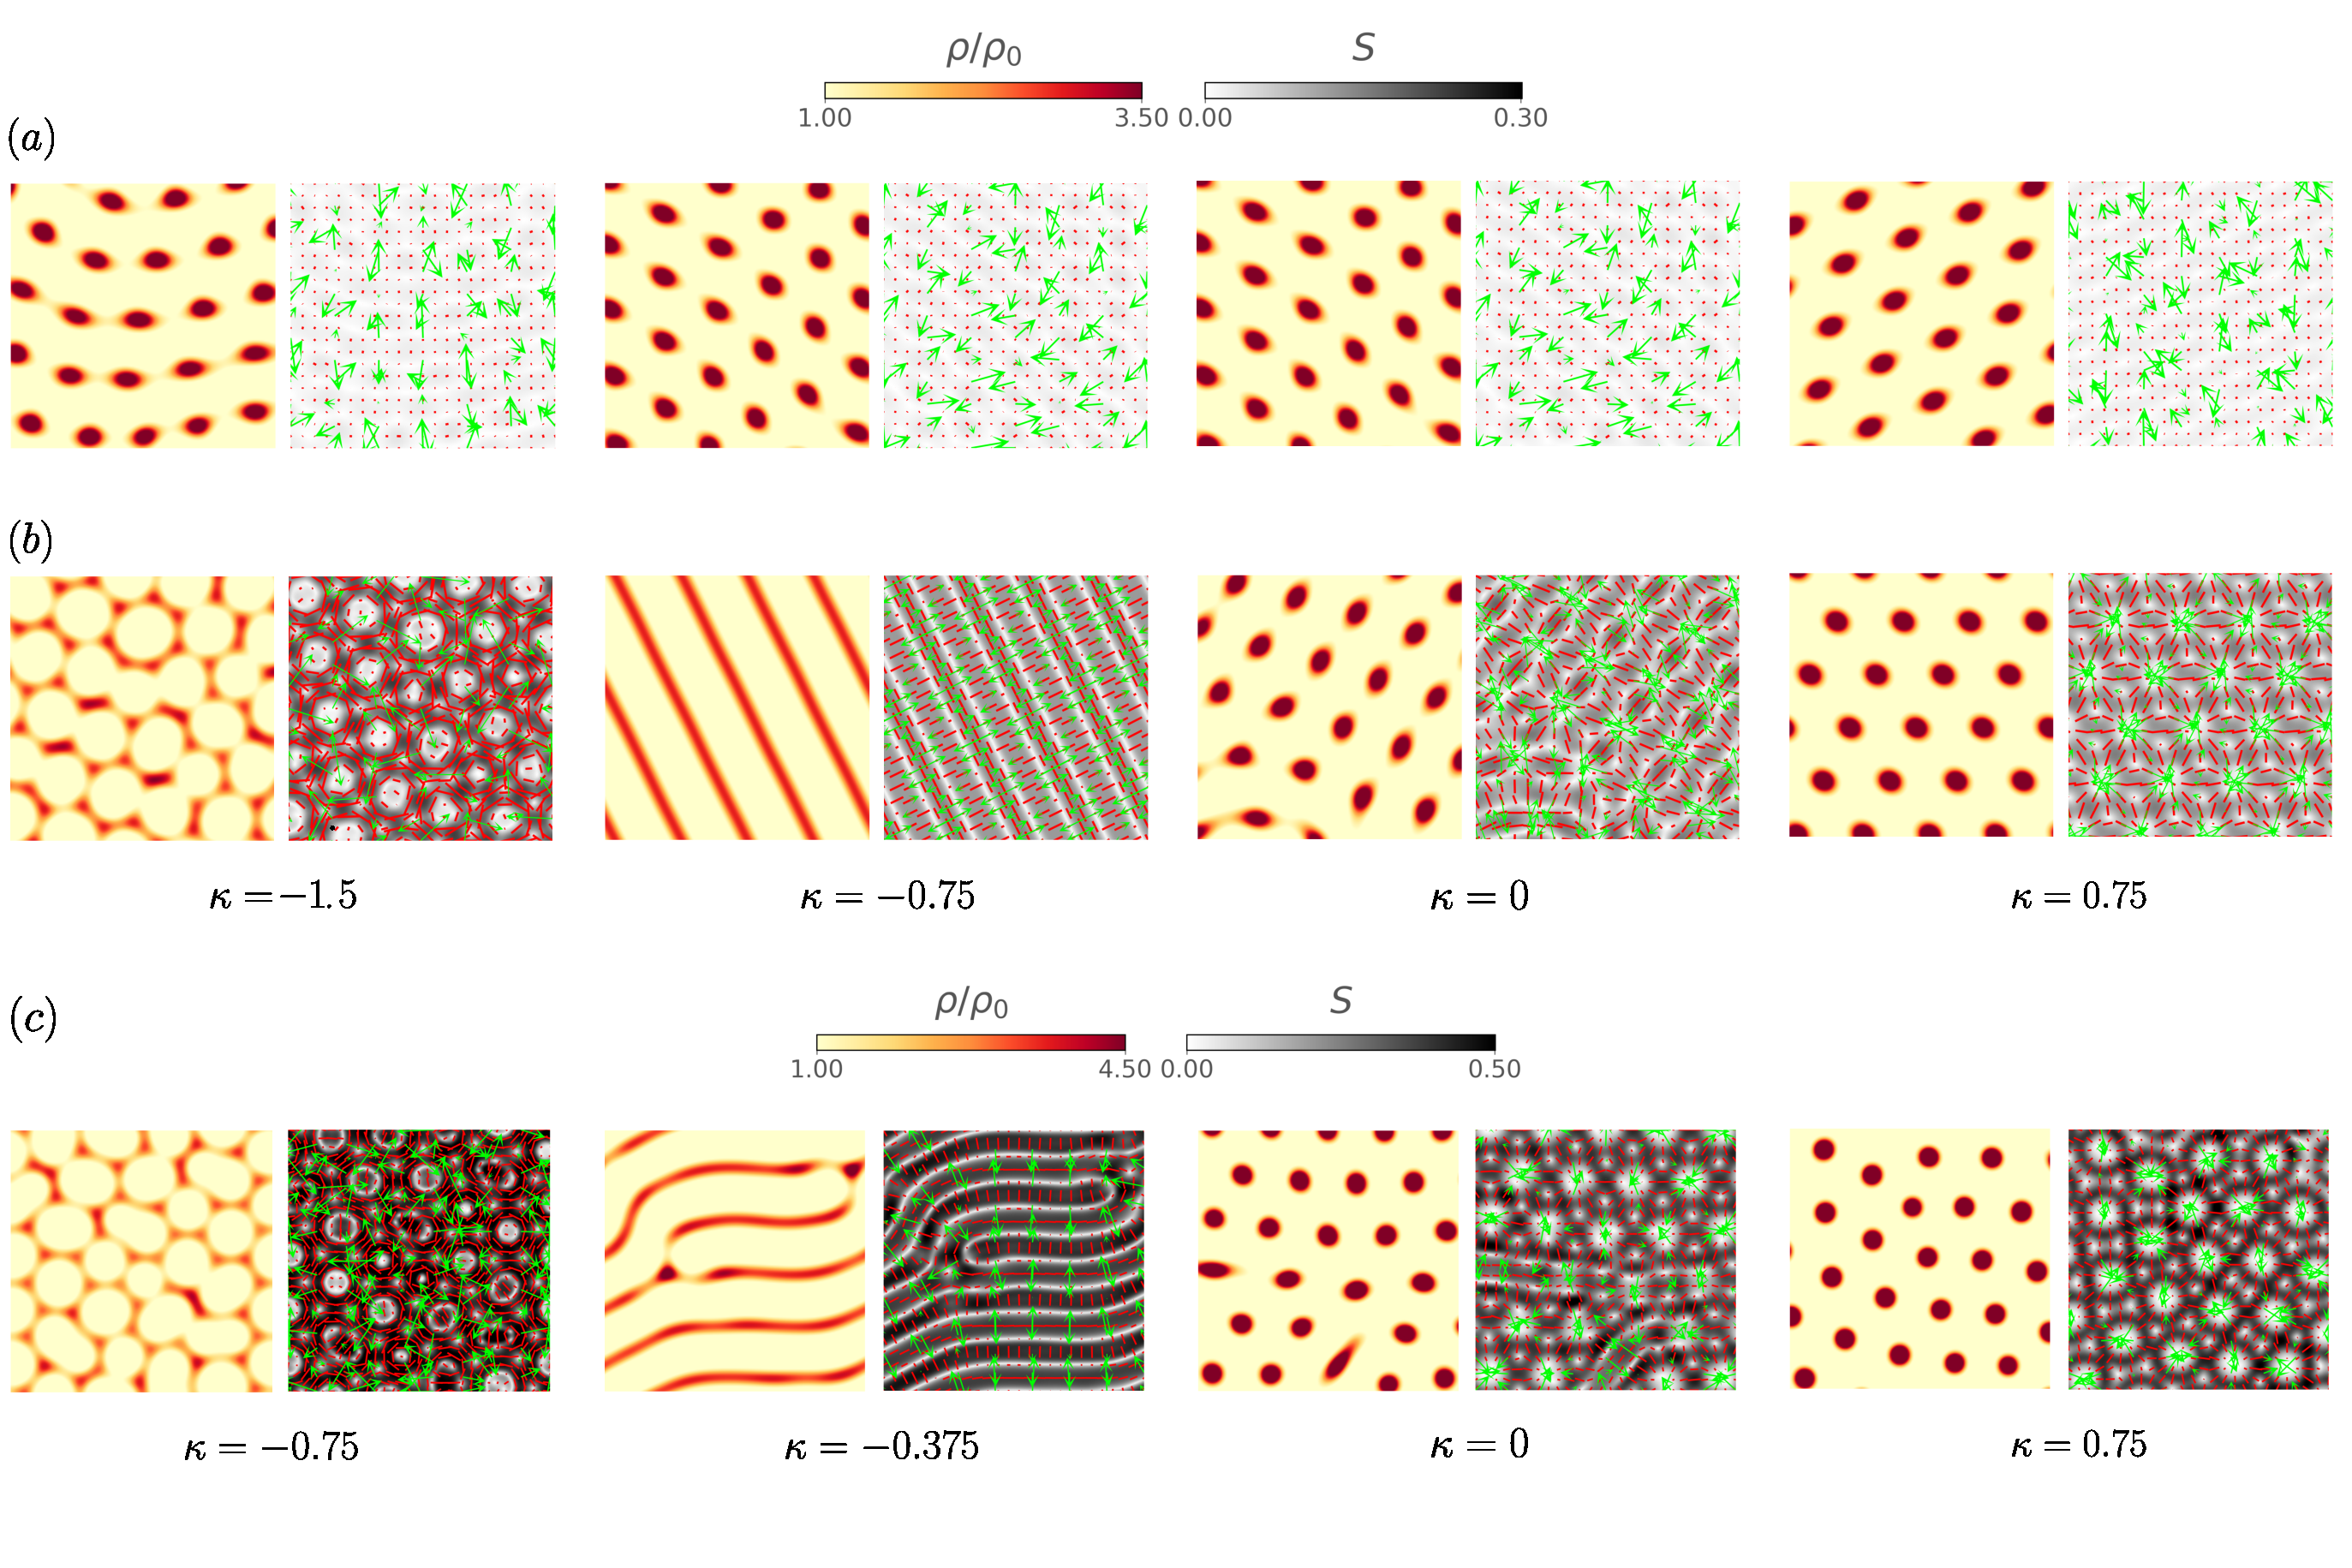
\includegraphics[width=\textwidth]{supplem_figure_1.pdf}
	\caption{\textbf{Pattern formation for a range of values of anisotropic active parameter $\kappa$ in the limit  $\lambda_{\odot} \rightarrow 0$.} (a) Pattern formation for canonical material parameters used in Fig.~\ref{fig4.2} except for  $\lambda_{\odot}=0$. (b) Here, in addition to  $\lambda_{\odot}=0$, we set $\beta^2 = 2\eta \eta_{\rm rot}$ to the largest value allowed by Onsager's inequality. (c) Using the parameters as in (b), we further increase friction as detailed in Table~\ref{defaulttable}.
	}
	\label{supplem_fig_1}
\end{figure}



\begin{figure}[p]
	\centering
	\includegraphics[width=0.95\textwidth]{supp_fig_stress.pdf}
		\caption{\textbf{Stress distribution along ($\sigma_{\vert\vert}$) and perpendicular to ($\sigma_{\perp}$) the dense nematic bundles.} The left column shows the density distribution, the middle column the total stress along and perpendicular to nematic bundles, and the right column the different contributions to the total stress dominated by  the active and the viscous components. In all cases, we consider for convenience fully nonlinear simulations in 1D to easily define the orthogonal directions relative to the self-organized pattern. (a) to (c) show patterns obtained for negative tension anisotropy $\kappa$ of increasing magnitude, whereas (d) shows a chaotic pattern resulting from a large hydrodynamic length. The modal parameters used in the plots are the same as in Figs.~\ref{fig4.2} and~\ref{fig4.3} and are described in Tables~\ref{defaulttable} and A.3. }
	\label{supplem_fig_2}
\end{figure}



\begin{figure}[p]
	\centering
	\includegraphics[width=0.65\textwidth]{supplem_figure_2.pdf}
	\caption{ \textbf{Discrete network simulations}. (I) Microstructural modeling approach using cytosim. (a) The nematic ordering of the network, $S$, measured with respect to a director $\hat{\bm{n}}$, is controlled by a system-wide restraining energy. (b) Actin filaments are represented by sets of connected particle points that are kept at a fixed distance (segmentation) and have finite bending rigidity $\kappa_A$. Crosslinkers are Hookean springs with stiffness $K_X$ and resting length $\ell_X$. Myosin motors are Hookean springs with stiffness $K_M$ and resting length $\ell_M$; their ends can `walk' on filaments at a speed $v_M$, which is affected by force application.  (II) Simulation protocol to quantify active tension anisotropy. (a) Initial fiber seeding without orientational bias. (b) Rearrangement of the network to provide a nematic orientation characterized by the ordering parameter $S_0$. (c) Introduction of anchors to measure the active forces exerted at the system's boundaries. (d) Introduction of crosslinkers and myosin motors and deactivation of the restraining potential, which drives the system out-of-equilibrium and allows us to track tensions at the boundary, (e,f). (III) Protocol to  quantifying the orientational activity parameter $\rho \lambda_{\odot}$. (a) Initial fiber seeding without orientational bias. (b) Athermal rearrangement of the network to provide a nematic orientation characterized by the ordering parameter $S_0$. (c) Estimation of the model parameter $\eta_{\rm rot}$, which characterizes the dynamics of athermal network reorientation in the presence of a restraining potential of stiffness $\mathcal{K}_S$; note that a single value of $\eta_{\rm rot}$  describes the system behavior for various $S_0$. (d) Introduction of crosslinkers and myosin motors, activation of system temperature, and deactivation of the restraining potential. The dynamics of orientational order of the system drive out-of-equilibrium are then tracked during a time period (d,e). }
	\label{supplem_fig_3}
\end{figure}

\section{Parameters used for the numerical studies}  \label{appendix_1_sec_9}
\begin{table}[H]
	\begin{tabular}{l|cccc} \textbf{Params.} &  Fig.~\ref{sec_1_chap_3_fig_1}    &  Fig.~\ref{sec_1_chap_3_fig_2}       &  Fig.~\ref{sec_1_chap_3_fig_3}      &  Fig.~\ref{sec_1_chap_3_fig_3.5}         \\ \hline 
		$\rho_0$ [\si{\micro \meter}]  & 0.2 & 0.2 & \textemdash & \textemdash  \\ 
		$\eta$ [\si{\pascal \second}] & $10^4$ & $10^4$ & $10^4$ & $10^4$  \\ 
		$\ell_s = \sqrt{\eta/\gamma}$ [\si{\micro \meter]} &10 &10&10 &10 \\
		$k_d$ [\si{\second}$^{-1}$] &0.1 & 0.1 & \textemdash & \textemdash\\
		$D$ [\si{\micro \meter}$^2$ s$^{-1}$] & 0.02& 0.02 & \textemdash & \textemdash \\
		$\eta_{\rm rot} / \eta$ & 1&1 & 1&1\\
		$\beta / \eta$ & -1 & -1,-0.1 & -0.2 & -0.2 \\
		$a/\eta$ $[\si{\second}^{-1}]$ & 1 &1  & -1 &-1 \\
		$b/\eta$ $[\si{\second}^{-1}]$  &4 &4  & 2 &2  \\
		$L/\eta$ $[\si{\micro \meter}^2  \si{\second}^{-1}$] & $ 0.01$&$ 0.01$ & [$8 \times 10^{-4}$ ,$0.18  $ ] & $8 \times 10^{-4}$  \\
		$\rho_0 \lambda_{\bigodot}^0 /(2a)$ &0.4  &0.2,0.4,0.6  & \textemdash & \textemdash  \\
		$\lambda^0/\eta \, [\si{\second}^{-1}]$ &0.12& 0.12  &\textemdash & \textemdash\\
		$\delta \lambda/ \lambda$   & 5& 5 &  \textemdash &  \textemdash\\
		$\kappa = \lambda_{\rm aniso}/\lambda$  & [0.5,2]  &1.0 & \textemdash &\textemdash,     \\
		$\lambda_{\rm aniso}/\eta [s^{-1}]$  & \textup{see value of} $\kappa$  &\textup{see value of} $\kappa$  & 0 &$8.9 \times 10^{-3}$, $0.036$,$0.08$,$0.32$     \\
		$\ell_0 $  [\si{\micro \meter}]  & 20  & 20 & 1  & 1 \\
		$\ell_a = \sqrt{L/\left(\lambda_{\rm aniso}S_0\right)}$   & \textemdash  & \textemdash & $\infty$  & $\infty, 0.3,0.15,0.1,0.05,0.04$ \\
		$$ [\si{\micro \meter}] & &  &   &  \\
		$\ell_p = \sqrt{L/(2|a|-\rho_0\lambda_{\odot})}$   & 0.056 &  0.0527,0.056,0.06   & [0.02, 0.3]  & 0.02 \\
		$$ [\si{\micro \meter}] & &  &   &  \\
		\hline 
	\end{tabular}
	\caption{Overview of parameters used for numerical studies of Chapter~\ref{chap_3}.}
	\label{modal_parameters}
	\end{table}

	\begin{table}[hb]
	\begin{center}\begin{tabular}{l|ccccc} Parameters & Fig.~\ref{fig4.2} & Fig.~\ref{supplem_fig_1}(a) & Fig.~\ref{supplem_fig_1}(b) & Fig.~\ref{supplem_fig_1}(c)     \\ \hline \\
			$\bar{k}_d$  &  0.1& 0.1 &0.1&0.01  \\
			$\bar{L}$  & 1 & 1 &1&1   \\
			$\bar{c}_0$  & 4&  4&4 &0.4 \\
			$\bar{b}$  & 20& 20&20&2\\
			$\bar{\eta}_{\rm rot}$  &  1&  1& 1&1 \\
			$\bar{\beta}$  &  -0.2&  -0.2&-$\sqrt{2}$&-$\sqrt{2}$  \\
			$\bar{\lambda}_\odot$ &  6& 0 &0&0  \\
			$\bar{\lambda}$ &$1.3 \bar{\lambda}_{\rm crit}$  & $1.3 \bar{\lambda}_{\rm crit}$&$1.3 \bar{\lambda}_{\rm crit}$&$1.3 \bar{\lambda}_{\rm crit}$  \\
			$\kappa$ & [-0.8,0.8] & [-1.5,-0.75,0,0.75]&[-1.5,-0.75,0,0.75]&[-0.75,-0.375,0,0.75]  \\
			$\ell_0$ & 8 & 8 &8&8  \\
			\hline
		\end{tabular}
	\end{center}
	\caption{Model parameters used in figures  of Chapter~\ref{chap_4}.}
	\label{defaulttable}
    \end{table}

	\begin{sidewaystable}
	\begin{minipage}[c][\textheight][c]{\textwidth}
		\begin{center}
			\begin{tabular}{l|cccccccccccc} Params.& 4.1 &  4.2 & 4.3(I,II) & 4.3(III,IV) & 4.4 & 4.5a(III) & 4.5b(II,III) & 4.5b(I)& 4.5a(II) \\ \hline \\
				$\bar{k}_d$  &0.01&0.1&  0.1& 0.1 &0.1&0.1&10,20&20& 0.1  \\
				$\bar{L}$  &1&1& 1 &1& 1 &1& 1 & 1& 1\\
				$\bar{c}_0$ &0.4&4 &  4& 4& 4& 4&4 &200&-0.05\\
				$\bar{b}$  &2&20& 20& 20&20& 20&20&4000&20\\
				$\bar{\eta}_{\rm rot}$ &0& 1&1 1&&  1&  1&1&1&1  \\
				$\bar{\beta}$ & 0&-0.2& -0.2,0 & -$\sqrt{2}$,-0.2&-0.2&-0.2&-0.2 &-0.2&-0.2 \\
				$\bar{\lambda}_\odot$ &0&6&  6& 6 &6&6&6&1800&10.05\\
				$\bar{\lambda}$ &1.3$\bar{\lambda}_{\rm crit}$&1.3$\bar{\lambda}_{\rm crit}$&1.3$\bar{\lambda}_{\rm crit}$  & 1.3$\bar{\lambda}_{\rm crit}$ & 1.3$\bar{\lambda}_{\rm crit}$& Same as Movie~4.1 & 1.3$\bar{\lambda}_{\rm crit}$&1.3$\bar{\lambda}_{\rm crit}$&1.3$\bar{\lambda}_{\rm crit}$  \\
				$\kappa$ &0&-0.2,0.05,0.7& -0.2 & 0.2&-0.2,-0.5,-0.8  &-0.2&-0.2&-0.2&-0.2\\
				$\ell_0$ &8&8&8 & 8 &8&Same as Movie~4.1&8 &8&8  \\
							\hline
			\end{tabular}
		\end{center}
				\caption{Model parameters used in movies of Chapter~\ref{chap_4}. Below the first column consist of the model parameters and the rest of the columns labeled as $4.$x corresponds to the movie number. The caption of each video is described in the Appendix~\ref{appendix_3}.}
						\label{supplem_table_2}
	\end{minipage}
\end{sidewaystable}

\begin{sidewaystable}
	\begin{minipage}[c][\textheight][c]{\textwidth}
		\begin{center}\begin{tabular}{lccccc} \multicolumn{2}{l}{\textbf{Reference}}  &  Geometry and size [ \si{\micro\meter}\textbf{ ]} & $kT$ \textbf{[ }\si{\pico\newton \micro\meter}\textbf{ ]} & Time step [ \si{\second}\textbf{ ]} & $\nu$ \textbf{[ }\si{\pascal \second}\textbf{ ]} \\ \hline \\
				
				\multicolumn{2}{l}{Present work}  & Square: $\ell = 5$ & 0 or 0.0042 & 0.005 & 1  \\
				
				\multirow{3}{*}{\cite{Cortes2020}} & MM1 & Rectangle: 2 $\times$ 0.2 & 0.0042 & 0.001 & 1 \\
				
				& MM4 & Rectangle: 9.424 $\times$ 1 & 0.0042 & 0.001 & 1 \\
				
				& MM3 \& MM5 & Circle: $R = 1.5$ & 0.0042 & 0.001 & 1 \\
				
				\multicolumn{2}{l}{Cortex simulations in  \cite{Wollrab2019}} & Square: $L = 8$ & 0.0042 & 0.002 & 0.18 \\
				
				\multicolumn{2}{l}{ \cite{Bun2018}} & Circle: $R = 10$ & 0.0042 & 0.01 or 0.1 & 0.3  \\
				
				\multicolumn{2}{l}{Model with turnover in  \cite{Belmonte2017}} & Square: $L = 16$ & 0.0042 & 0.001 & 0.1 \\
				
				\multicolumn{2}{l}{ \cite{Descovich2017}} & Circle: $R = 15$ & 0.0042 & 0.002 & 1 \\
				
				\multicolumn{2}{l}{\cite{Ding2017}} & Circle: $R = 10$ & 0.0042 & 0.001 & 0.1 \\
				
				\multicolumn{2}{l}{\cite{Ennomani2016}} & Ring: $R = 4.5$, $t \approx 0.5 $ & 0.0042 & 0.01 & 0.18 \\
				
			\end{tabular}
		\end{center}
			\caption{Global parameters adopted in this study and in previous microstructural models that used cytosim.}
		\label{tab:GlobalParamTable}
	\end{minipage}
\end{sidewaystable}

\begin{sidewaystable}
	\begin{minipage}[c][\textheight][c]{\textwidth}

		\begin{center}
			\begin{tabular}{lcccccc} \multicolumn{2}{l}{\textbf{Reference}} & $\ell_A$ \textbf{[ }\si{\micro\meter}\textbf{ ]} & $\rho_A$ \textbf{[ }\si{\micro\meter/\micro\meter}$^{2}$\textbf{ ]} & $s_A$ \textbf{[ }\si{\micro\meter}\textbf{ ]} & $\kappa_A$ \textbf{[ }\si{\pico\newton \micro\meter}$^{2}$\textbf{ ]} & $r_A$ \textbf{[ }\si{\%/\second}\textbf{ ]} \\ \hline \\
				
				\multicolumn{2}{l}{Present work}  & 1.3 & 78, 156, or 234 & 0.2 & 0.1 & 20  \\
				
				\multirow{4}{*}{Ref. \cite{Cortes2020}} & MM1 & 2 & 1800 & $0.05 - 0.1$ & 0.06 & 0 \\
				
				& MM3 & $1.3 \pm 0.3$ & $50.9 - 81.5$ & $0.05 - 0.1$ & 0.06 & 0 \\
				
				& MM4 & $1.3 \pm 0.3$ &  $38.2 - 61.1$ & $0.05 - 0.1$ & 0.06 & 0 \\
				
				& MM5 & $1.3 \pm 0.3$ &  $50.9 - 81.5$ & $0.05 - 0.1$ & 0.06 & 0 \\
				
				\multicolumn{2}{l}{Cortex simulations in Ref. \cite{Wollrab2019}} & $0.1 - 4.0$ & $5.5 - 218.8$ & $0.1 - 0.4$ & 0.075 & 0 \\
				
				\multicolumn{2}{l}{Ref. \cite{Bun2018}} & 1.5 & 23.9 & 0.15 & 0.07 & 0  \\
				
				\multicolumn{2}{l}{Model with turnover in Ref. \cite{Belmonte2017}} & 5 & 27.3 & $0.1 - 0.2$ & 0.075 & $1.1 - 18.3$ \\
				
				\multicolumn{2}{l}{Ref. \cite{Descovich2017}} & $1.3 \pm 0.3$ & $3.4 - 5.4$ & 0.1 & 0.06 & 0 \\
				
				\multicolumn{2}{l}{Ref. \cite{Ding2017}} & $2.2$ & 35 & \textemdash & 0.05 & 0 \\
				
				\multicolumn{2}{l}{Ref. \cite{Ennomani2016}} & $0.95 - 1.75$ & $117.2 - 154.2$ & \textemdash & $0.042 - 0.063$ & 0 \\
				
			\end{tabular}
		\end{center}
			\caption{Actin filament parameters adopted in this study and in previous microstructural models that used cytosim.}
		\label{tab:ActinParamTable}
	\end{minipage}
\end{sidewaystable}

	\begin{sidewaystable}
	\begin{minipage}[c][\textheight][c]{\textwidth}
		\begin{center}\begin{tabular}{lcccccccccc}
				\multicolumn{2}{l}{\multirow{2}{*}{\textbf{Reference}}} & $\rho_M$ & $K_M$ & $\ell_M$ & $r_M^b$ & $d_M^b$ & $r_M^{u,0}$ & $f_M^u$ & $f_M^{\rm stall}$ & $v_M^{\rm max}$ \\
				
				\multicolumn{2}{l}{}  &  \textbf{[ }\si{1/\micro\meter} actin\textbf{ ]} & \textbf{[ }\si{\pico\newton/\micro\meter}\textbf{ ]} & \textbf{[ }\si{\micro\meter}\textbf{ ]} & \textbf{[ }\si{1/\s}\textbf{ ]} & \textbf{[ }\si{\micro\meter}\textbf{ ]} & \textbf{[ }\si{1/\second}\textbf{ ]} & \textbf{[ }\si{\pico\newton}\textbf{ ]} & \textbf{[ }\si{\pico\newton}\textbf{ ]} & \textbf{[ }\si{\micro\meter/\second}\textbf{ ]} \\ \hline \\
				
				\multicolumn{2}{l}{Present work}  & 0.8 & 250 & 0 & 50 & 0.02 & 50 & $\infty$ & 6 & 0.3 \\
				
				\multirow{2}{*}{\cite{Cortes2020}} &  & 0.5 & 100 & 0.3 & $0.2 - 3.6$ & $0.06 - 0.12$ & $0.8 - 1.71$ & 5 & $3.85 - 15$ & $0.137 - 0.6$ \\
				
				&& $0.6 - 1.0$ & 100 & 0.3 & $0.2 - 3.6$ & $0.06 - 0.12$ & $0.8 - 1.71$ & 5 & $3.85 - 15$ & $0.137 - 0.6$ \\
				
				\multicolumn{2}{l}{Cortex simulations} & $2 - 64$ & 100 & 0 & 10 & 0.01 & 0.5 & $\infty$ & 4 & 2  \\
					
	\multicolumn{2}{l}{ \cite{Wollrab2019}} &  &  &  &  &  &  &  &  &   \\			
				\multicolumn{2}{l}{Ref. \cite{Bun2018}} & 2.7 & 250 & 0.01 & 10 & 0.01 & 0.1 & 3 & 6 & 0.02 \\
				
				\multicolumn{2}{l}{Model with turnover } & 3.2 & 500 & 0 & 10 & 0.01 & 0.3 & $\infty$ & 6 & 0.2 \\
				\multicolumn{2}{l}{\cite{Belmonte2017}} & &  &  &  & & &  &  & \\				
				\multicolumn{2}{l}{\cite{Descovich2017}} & $0.5 - 0.8$ & 1'400 & 0.32 & 0.2 & 0.33 & 0.3 & 3.85 & 24.5 & 0.1 \\
				
				\multicolumn{2}{l}{\cite{Ding2017}} & 0 or 5.8 & 250 & 0 & 10 & 0.01 & 0.5 & $\infty$ & 6 & 0.5 \\
				
				\multicolumn{2}{l}{\cite{Ennomani2016}} & $0.3 - 0.4$ & 100 & 0.03 & 5 & 0.05 & 0 & 3.65 & 2 & 0.3 \\
				
			\end{tabular}
		\end{center}
			\caption{Myosin motor parameters adopted in this study and in previous microstructural models that used cytosim.}
		\label{tab:MotorParamTable}
	\end{minipage}
\end{sidewaystable}

\hspace{1cm}





	
	

	
	\renewcommand{\thesection}{B.\arabic{section}}
	\chapter{Active self-organization of a nematic gel on a deformable curved surface} \label{appendix_2}
	\section{Covariant derivative} \label{velocity_gradient}

We denote by $\nabla^{\rm 3D} \bm{V}$ the three-dimensional gradient of a vector $\bm{V}$. In general curvilinear coordinates, the gradient is given by
\begin{equation}
	\nabla^{\rm 3D}_\beta V^\alpha = \partial_\beta V^\alpha + \bar{\Gamma}^\alpha_{\beta\gamma} V^\gamma.
\end{equation} 
where $\bar{\Gamma}^\alpha_{\beta\gamma} = \bm{e}^\alpha \cdot \partial_\beta \bm{e}_\gamma$. We are interested in the projection of this derivative onto $A$, which we call $\nabla \bm{V}$
\begin{equation}
	\nabla \bm{V} = \nabla^{\rm 3D} \bm{V}\,\mathbb{P}.
\end{equation} 
where $\mathbb{P}$ is the projector onto $A$. To calculate $\nabla\bm{V}$, we introduce a basis of Cartesian space on $A$ given by $\bm{e}_1$, $\bm{e}_2$ and $\bm{N}$ (the two tangent vectors to $A$ and the normal). In this basis,
\begin{equation}
	\nabla_a V^\alpha = \nabla^{\rm 3D}_a V^\alpha .
\end{equation} 
and we have 
\begin{equation}
	\bar{\Gamma}^a_{bc} = \Gamma^a_{bc},\quad \bar{\Gamma}^3_{ab} = -k_{ab},\quad \bar{\Gamma}^a_{3b} = k^a_b,\qquad \Gamma^3_{3a}=\Gamma^3_{a3}=\Gamma^a_{33}=\Gamma^3_{33} = 0.
\end{equation}
We split the calculation of $\nabla\bm{V}$ into its tangential and normal components. The tangential part leads to
\begin{equation}
	\nabla^{\rm 3D}_b v^a =  \partial_b v^a + \bar{\Gamma}^a_{b\gamma} V^\gamma = \partial_b v^a + \bar{\Gamma}^a_{bc} v^c + \bar{\Gamma}^a_{b3} v_n = \nabla_b v^a + k^a_b v_n.
\end{equation}
Similarly,
\begin{equation}
	\nabla^{\rm 3D}_b v_n =  \partial_b v^3 + \bar{\Gamma}^3_{b\gamma} V^\gamma = \partial_b v_n + \bar{\Gamma}^3_{bc} v^c = \nabla_b v_n - k_{bc} v^c.
\end{equation}
Putting these results together,
\begin{equation}
	\nabla \bm{V} = \left(\nabla_b v^a+v_n k_b{}^a \right) \bm{e}_a \otimes \bm{e}^b + \left(\nabla_a v_n - k_{ab} v^b \right) \bm{n} \otimes \bm{e}^a.
\end{equation}
In the case $v_n=0$, i.e. for a tangent vector, this definition does not coincide with the usual covariant derivative. To get the covariant derivative, we need to project once more to eliminate the normal terms
\begin{equation}
\nabla\bm{v} = \mathbb{P}\,\nabla^{\rm 3D} \bm{V}\,\mathbb{P} = \nabla\bm{v}.
\end{equation}

\section{Lie derivative of curvature tensor} \label{curvature_tensor}
The Lie derivative of curvature tensor is given by \cite{capovilla2002, salbreux2017}
\begin{equation} \label{append_1_II}
	\mathcal{L}_v k_{ab} = -\nabla_a \nabla_b v_N + k_{ac} \nabla_b v^c + k_{bc}\nabla_a v^c + \nabla_a k_{bc}v^c + v_Nk_{ac}k^{c}_{~b},
\end{equation}
which can be related to $\bm{\zeta}$ and $\bm{d}$ as
\begin{align} \label{append_2_II}
	\mathcal{L}_v k_{ab}  & = -\frac{1}{2}\nabla_a \bigg(\nabla_b v_N -  k_{bc} v^c\bigg) - \frac{1}{2}\nabla_b \bigg(\nabla_a v_N -  k_{ac} v^c\bigg) + \frac{1}{2}\bigg( \frac{\nabla_b v^c + \nabla^c v_b}{2} + v_Nk_{~b}^c \bigg)k_{ac}   \nonumber \\ & + \frac{1}{2}\bigg( \frac{\nabla_a v^c +   \nabla^c v_a}{2} +v_N k^{c}_{~a} \bigg)k_{bc} + \frac{1}{2}k_{bc}(\nabla_a v^c -   \nabla^c v_a) +  \frac{1}{2}k_{ac}(\nabla_b v^c -   \nabla^c v_b) \nonumber \\ & =
	\frac{1}{2} \epsilon_{b}^{~c} (-\nabla_a \omega_c - k_{ac} \omega_N ) + \frac{1}{2} \epsilon_{a}^{~c} (-\nabla_b \omega_c - k_{bc}\omega_N) + \frac{1}{2}(d^c_{~b}k_{ac} +d^c_{~a}k_{bc})  \nonumber \\ & =-\frac{1}{2} \left(\zeta_{ab} +\zeta_{ba}\right)+ \frac{1}{2}\left(d^c_{~b}k_{ac} +d^c_{~a}k_{bc}\right),
\end{align}
where we have used $ \nabla_a k_{cb} = \nabla_b k_{ca}  = \nabla_c k_{ab}$, also known as Codazzi-Mainardi equation.
 \iffalse 
\section{Change in basis}
 We derive the analytical expression of a transformation matrix $T_{[\phi,\varphi]~a}^{\quad \,\, A}$ that establish a map between the local monge basis $\partial_A \bm{\varphi}= \bm{j}_{A\{I\}} + \partial h_{\{I\}}/\partial \theta^A \bm{j}_{3\{I\}}$ and the tangent basis $\partial_a \bm{\phi}$, that is,
 \begin{equation} \label{B.18}
\partial_a \bm{\phi} = T_{[\phi,\varphi]~a}^{\quad \,\, A} \partial_A \bm{\varphi}.
 \end{equation}
After multiplying $\bm{j}_{B\{I\}}$ with the definition of $\partial_A \bm{\varphi}$ we get
\begin{equation} \label{B.19}
 \partial_A \bm{\varphi} \cdot \bm{j}_{B\{I\}} = \delta_{AB}
\end{equation}
Thus, after multiplying $\bm{j}_{B\{I\}}$ with eq.~(\ref{B.18}) and  substituting the equation above
\begin{equation} \label{B.20}
T_{[\phi,\varphi]~a}^{\quad \,\, A} \delta_{AB}= 	\partial_a \bm{\phi} \cdot  \bm{j}_{B\{I\}}
\end{equation}


\section{Auxiliary quantities in weak formulation of inextensible active nematic model}

\begin{equation} \label{B.21}
	\frac{\delta q^{[\textup{n}]}_{ab}}{\delta q_{C\{K\}}^{[\textup{n}]}} = \underset{K \in \langle E_{\{K\}} \rangle}{\mathrm{\sum}} B_{\{K\}}L_{~AB\{ K \}}^{C[n]} T_{[\phi,\varphi]~a}^{\quad \,\, A}  T_{[\phi,\varphi]~b}^{\quad \,\, B} ,
\end{equation}


\begin{align} \label{B.22}
	\frac{\delta \left( \nabla_c q^{ab [\textup{n}]}\right)}{\delta q_{C\{K\}}^{[\textup{n}]}}  = & \underset{K \in \langle E_{\{K\}} \rangle}{\mathrm{\sum}}\left\{\partial_cB_{\{K\}}^{~s} T_{[\phi,\varphi]~a}^{~~~~A} T_{[\phi,\varphi]~b}^{~~~~B} L_{~AB\{K\}}^{C[n]}  + B_{\{K\}}^{~s} \partial_cT_{[\phi,\varphi]~a}^{~~~~A} \nonumber T_{[\phi,\varphi]~b}^{~~~~B}  L_{~AB\{K\}}^{C[n]}  \right. \\
	&\left.+\,B_{\{K\}}^{~s} T_{[\phi,\varphi]~a}^{~~~~A} \partial_cT_{[\phi,\varphi]~b}^{~~~~B}  L_{~AB\{K\}}^{C[n]}  +B_{\{K\}}^{~s}  T_{[\phi,\varphi]~a}^{~~~~A} T_{[\phi,\varphi]~b}^{~~~~B}\partial_c  L_{~AB\{K\}}^{C[n]} \right\}, 
\end{align}

\begin{equation} \label{B.23}
	\frac{\delta \widehat{q}_{ab}^{[\textup{n}]}}{\delta x_{C\{ K\}}^{[\textup{n}]}} =  \frac{2}{\Delta t^{[\textup{n}]}} q_{b}^{\,i[\textup{n-1}]} \frac{\delta g^{[\textup{n}]}_{ia}}{\delta  x_{C{\{K\}}}^{[\textup{n}]}} ,
\end{equation}
 
\begin{equation} \label{B.24}
	\frac{\delta g^{[\textup{n}]}_{ab}}{\delta  x_{C{\{K\}}}^{[\textup{n}]}} = 2 \frac{\delta \bm{e}_a^{[\textup{n}]}}{\delta   x_{C\{K\}}^{[\textup{n}]}}   \cdot \bm{e}_b^{[\textup{n}]},
\end{equation}

\begin{equation} \label{B.25}
	\frac{\delta e_{a}^{\,A[\textup{n}]}}{\delta  x_{\{K\}}^{\,C[\textup{n}]}} =  \partial_{a} B^s_{\{K\}}  \delta^{AC}.
\end{equation}



%%%%


\begin{equation} \label{B.26}
	\frac{ \delta S^{2[\textup{n}]}}{\delta  \bm{x}_{\{K\}}^{[\textup{n}]}}  =  2\left(q^{ab[\textup{n}]}\frac{\delta q_{ab}^{[\textup{n}]}}{\delta  \bm{x}_{\{K\}}^{[\textup{n}]}} + q_{ab}^{[\textup{n}]}\frac{\delta q^{ab[\textup{n}]}}{\delta  \bm{x}_{\{K\}}^{[\textup{n}]}}  \right),
\end{equation}

\begin{equation} \label{B.27}
	\frac{\delta q^{ab[\textup{n}]}}{\delta  \bm{x}_{\{K\}}^{[\textup{n}]}} = g^{ae[\textup{n}]}g^{bf[\textup{n}]}  \frac{\delta q_{ef}^{[\textup{n}]}}{\delta  \bm{x}_{\{K\}}^{[\textup{n}]}} + 2   \frac{\delta g^{ae[\textup{n}]}}{\delta  \bm{x}_{\{K\}}^{[\textup{n}]}} g^{bf[\textup{n}]} q_{ef}^{[\textup{n}]},
\end{equation}

\begin{equation} \label{B.28}
	\frac{\delta q_{ab}^{[\textup{n}]}}{\delta  \bm{x}_{\{K\}}^{[\textup{n}]}} =\underset{K \in \langle E_{\{K\}} \rangle }{\mathrm{\sum}} B_{\{K\}}^s\frac{\delta q_{AB\{K\}}}{\delta \bm{x}_{\{K\}}^{[\textup{n}]}} T_{[\phi,\varphi]~a}^{\quad \,\, A}  T_{[\phi,\varphi]~b}^{\quad \,\, B} ,
\end{equation}


\begin{equation} \label{B.29}
	\frac{\delta q_{AB\{K\}}}{\delta \bm{x}_{\{K\}}^{[\textup{n}]}} =  B_{\{K\}}^s \partial_{\bm{x}_{\{K\}}^{[\textup{n}]}}L_{~AB\{K\}}^{C[\textup{n}]}q_{C\{K\}} T_{[\phi,\varphi]~a}^{\quad \,\, A}  T_{[\phi,\varphi]~b}^{\quad \,\, B} ,
\end{equation}

\begin{equation} \label{B.30}
	\partial_{\bm{x}_{\{K\}}^{[\textup{n}]}}  L_{~11}^{1^{[\textup{n}]}} =  \frac{\partial_{\bm{x}_{\{K\}}^{[\textup{n}]}}  g^{22^{[\textup{n}]}} g^{11^{[\textup{n}]}} - \partial_{\bm{x}_{\{K\}}^{[\textup{n}]}}g^{11^{[\textup{n}]}}g^{22^{[\textup{n}]}}}{\left(g^{22^{[\textup{n}]}}\right)^2},
\end{equation}

\begin{equation} \label{B.31}
	\partial_{\bm{x}_{\{K\}}^{[\textup{n}]}}  L_{~11}^{2^{[\textup{n}]}} = 2 \frac{\partial_{\bm{x}_{\{K\}}^{[\textup{n}]}} g^{22^{[\textup{n}]}}g^{12^{[\textup{n}]}} - \partial_{\bm{x}_{\{K\}}^{[\textup{n}]}} g^{12^{[\textup{n}]}}g^{22^{[\textup{n}]}}}{\left(g^{22^{[\textup{n}]}}\right)^2}, \quad \partial_{\bm{x}_{\{K\}}^{[\textup{n}]}}  L_{~AB\{K\}}^{C^{[\textup{n}]}} = 0 \text{ otherwise},
\end{equation}

\begin{equation} \label{B.32}
	g^{AB^{[\textup{n}]}} = T_{[\phi,\varphi]~a}^{~~~~A{[\textup{n}]}} T_{[\phi,\varphi]~b}^{~~~~B{[\textup{n}]}}g^{ab{[\textup{n}]}} ,
\end{equation}

\begin{equation} \label{B.33}
	\partial_{\bm{x}_{\{K\}}^{[\textup{n}]}} g^{AB{[\textup{n}]}} =  T_{[\phi,\varphi]~a}^{~~~~A{[\textup{n}]}} T_{[\phi,\varphi]~b}^{~~~~B{[\textup{n}]}} \partial_{\bm{x}_{\{K\}}^{[\textup{n}]}}g^{ab{[\textup{n}]}}.
\end{equation}


%%%%

\begin{gather} \label{B.33}
	\frac{\delta  \left(\partial_c q_{ab}^{[\textup{n}]}\right)}{\delta  \bm{x}_{\{K\}}^{[\textup{n}]}} =  \sum_{I\in\langle E_{\{K\}} \rangle} \left\{\partial_cB_{\{K\}}^{s} T_{[\phi,\varphi]~a}^{~~~~A} T_{[\phi,\varphi]~b}^{~~~~B} \delta_{\bm{x}_{\{K\}}^{[\textup{n}]}} L_{~AB\{K\}}^{C[\textup{n}]} q_{C\{K\}} + B_{\{K\}}^{s} \partial_cT_{[\phi,\varphi]~a}^{~~~~A} T_{[\phi,\varphi]~b}^{~~~~B} \delta_{\bm{x}_{\{K\}}^{[\textup{n}]}} L_{~AB\{K\}}^{C[\textup{n}]} q_{C\{K\}} \right. \nonumber +\\
	\left.\,B_{\{K\}}^{s} T_{[\phi,\varphi]~a}^{~~~~A} \partial_cT_{[\phi,\varphi]~b}^{~~~~B} \delta_{\bm{x}_{\{K\}}^{[\textup{n}]}} L_{~AB\{K\}}^{C[\textup{n}]} q_{C\{K\}} +B_{\{K\}}^{s}  T_{[\phi,\varphi]~a}^{~~~~A} T_{[\phi,\varphi]~b}^{~~~~B}\delta_{\bm{x}_{\{K\}}^{[\textup{n}]}} \partial_c  L_{~AB\{K\}}^{C[\textup{n}]}q_{C\{K\}}\right\},
\end{gather}

\begin{gather}  \label{B.34}
	\delta_{\bm{x}_{\{K\}}^{[\textup{n}]}} \partial_c  L_{~11}^1 =  -2\frac{\partial_c g^{22[\textup{n}]} g^{11[\textup{n}]} - \partial_cg^{11[\textup{n}]}g^{22[\textup{n}]}}{\left(g^{22[\textup{n}]}\right)^3} \delta_{\bm{x}_{\{K\}}^{[\textup{n}]}} g^{22[\textup{n}]} +   \frac{\delta_{\bm{x}_{\{K\}}^{[\textup{n}]}} \partial_c g^{22[\textup{n}]} g^{11[\textup{n}]} - \delta_{\bm{x}_{\{K\}}^{[\textup{n}]}}  \partial_cg^{11[\textup{n}]}g^{22[\textup{n}]}}{\left(g^{22[\textup{n}]}\right)^2} + \nonumber \\ \qquad \qquad \quad
	\frac{ \partial_c g^{22[\textup{n}]}\delta_{\bm{x}_{\{K\}}^{[\textup{n}]}} g^{11[\textup{n}]} - \partial_cg^{11[\textup{n}]}\delta_{\bm{x}_{\{K\}}^{[\textup{n}]}}g^{22[\textup{n}]}}{\left(g^{22[\textup{n}]}\right)^2},
\end{gather}


\begin{gather}  \label{B.35}
	\delta_{\bm{x}_{\{K\}}^{[\textup{n}]}} \partial_c  L_{~11}^2 =  -4\frac{\partial_c g^{22[\textup{n}]} g^{12[\textup{n}]} - \partial_cg^{12[\textup{n}]}g^{22[\textup{n}]}}{\left(g^{22[\textup{n}]}\right)^3} \delta_{\bm{x}_{\{K\}}^{[\textup{n}]}} g^{22[\textup{n}]} +   2\frac{\delta_{\bm{x}_{\{K\}}^{[\textup{n}]}} \partial_c g^{22[\textup{n}]} g^{12[\textup{n}]} - \delta_{\bm{x}_{\{K\}}^{[\textup{n}]}}  \partial_cg^{12[\textup{n}]}g^{22[\textup{n}]}}{\left(g^{22[\textup{n}]}\right)^2} + \nonumber \\ \qquad \qquad \quad
	2\frac{ \partial_c g^{22[\textup{n}]}\delta_{\bm{x}_{\{K\}}^{[\textup{n}]}} g^{12[\textup{n}]} - \partial_cg^{12[\textup{n}]}\delta_{\bm{x}_{\{K\}}^{[\textup{n}]}}g^{22[\textup{n}]}}{\left(g^{22[\textup{n}]}\right)^2},
\end{gather}
and otherwise $  \delta_{\bm{x}_{\{K\}}^{[\textup{n}]}} \partial_c  L_{~AB\{K\}}^C = 0$.

\begin{gather} \label{B.36}
	\delta_{\bm{x}_{\{K\}}^{[\textup{n}]}} \partial_cg^{AB[\textup{n}]} = \partial_cT_{[\phi,\varphi]~a}^{~~~~A} T_{[\phi,\varphi]~b}^{~~~~B}\delta_{\bm{x}_{\{K\}}^{[\textup{n}]}}g^{ab[\textup{n}]} + T_{[\phi,\varphi]~a}^{~~~~A} \partial_cT_{[\phi,\varphi]~b}^{~~~~B}\delta_{\bm{x}_{\{K\}}^{[\textup{n}]}}g^{ab[\textup{n}]} +  \\ \qquad \qquad \qquad T_{[\phi,\varphi]~a}^{~~~~A} T_{[\phi,\varphi]~b}^{~~~~B} \delta_{\bm{x}_{\{K\}}^{[\textup{n}]}} \partial_cg^{ab[\textup{n}]}.  \nonumber
\end{gather}


\begin{align}  \label{B.37}
	\delta_{\bm{x}_{\{K\}}^{[\textup{n}]}}  \partial_cg^{ab[\textup{n}]} & = -\bigg(g^{ad[\textup{n}]}g^{be[\textup{n}]}  \delta_{\bm{x}_{\{K\}}^{[\textup{n}]}} \partial_c g_{de}^{[\textup{n}]}+ g^{ad[\textup{n}]} \delta_{\bm{x}_{\{K\}}^{[\textup{n}]}} g^{be[\textup{n}]} \partial_c g_{de}^{[\textup{n}]} +  \\ & \qquad \delta_{\bm{x}_{\{K\}}^{[\textup{n}]}} g^{ad[\textup{n}]}g^{be[\textup{n}]} \partial_c g_{de}^{[\textup{n}]}\bigg), \nonumber
\end{align}

\begin{equation}  \label{B.38}
	\partial_cg_{ab}^{[\textup{n}]} =   \sum_{K\in\langle E_{\{k\} \}}\rangle} \left\{ \partial_c\partial_aB_{J}^s\cdot \partial_bB_{J}^s+ \partial_aB_{J}^s \cdot \partial_c\partial_bB_{J}^s \right\} d A^{[\text{n}]} .
\end{equation}

 \fi
\section{Modal parameters used in cytoskeleton surface simulations}

\begin{table}[H]
	\resizebox{\columnwidth}{!}{\begin{tabular}{l|cccccccccc} \textbf{Model parameters} & Fig.~\ref{fig_2_III} & Fig.~\ref{fig_3_III}(a)& Fig.~\ref{fig_3_III}(b)& Fig.~\ref{fig_3_III}(c) & Fig.~\ref{fig_8_III}(a) & Fig.~\ref{fig_8_III}(b) & Fig.~\ref{fig_8.1_III} & Fig.~\ref{fig_5_III}     \\ \hline 
			$\rho_0$ [\si{\micro \meter}]  & 0.2 & 0.2 & 0.2 & 0.2 & 0.2 & 0.2 & 0.2 &0.2  \\ 
			$\eta$ [\si{\pascal \second}] & $10^4$ & $10^4$ & $10^4$  & $10^4$ & $10^4$ & $10^4$ & $10^4$  & $10^4$   \\ 
			$\ell_s$ [\si{\micro \meter]} &10 &10 &10 & 10&10 & 10 & 10 & 10  \\
			$k_d$ [\si{\second}$^{-1}$] &0.1 & 0.1 & 0.1 & 0.1&0.1&0.1 & 0.1 & 0.1  \\
			$D$ [\si{\micro \meter}$^2$ s$^{-1}$] & 0.04& 0.04& 0.04 & 0.04 & 0.04&0.04 & 0.04  & 0.04  \\
			$\eta_{\rm rot} / \eta$ & 1&1 &1 & 1&1 &1 & 1 & 1 \\
			$\beta / \eta_{\rm rot}$ & -0.2 & -0.2 & -0.2 &-0.2&-0.2&-0.2 & -0.2 & -0.2 \\
			$a/\eta_{\rm rot}$ $[\si{\second}^{-1}]$ & 1. &1 &1&1&1&1 & 1 & 1 \\
			$b/\eta_{\rm rot}$ $[\si{\second}^{-1}]$  &16. &16 &16&16&16&16 & 16 & 16  \\
			$L/\eta_{\rm rot}$ $[\si{\micro \meter}^2  \si{\second}^{-1}$] & 0.01&0.01 & 0.01 &0.01&0.01& 0.01 & 0.01 & 0.01  \\
			$h(\rho_0) \lambda_\odot^0 /(2a)$ &0.04  &0.04 & 0.04&[0.04,0.08]&0.5&0.05 & 0.5  & 0.5   \\
			$\lambda^0/\eta [\si{\second}^{-1}]$ &0.1& 0.1&0.1& 0.1&2&2 & 2 & 2  \\
			$\delta \lambda/ \lambda^0$   & 12.5& 10& $[12.5,17.5]$&12.5&0&0 & 0  & 0 \\
			$\kappa$  & 1  &[0,2] & $[0,1.5]$ & [0.25,1.5]&1.5&1.5 & 0 & 0.75\\
			$R_0 [\si{\micro \meter}]$  & 5&5 & 5& 5&5&5 &5 & 5 \\
			$w/s$   & 0.02&0.02 & 0.02&0.02 &0&0 & 0 & 0 \\
			$\mathcal{B}/\eta [\si{\micro \meter}^2  \si{\second}^{-1}]$   & 0.01&0.01 & 0.01&0.01 &0.01&0.01 &0.01 &0.01   \\
			$\rho_s [\si{\micro \meter} ]$   &1&1 & 1&1 &1&$	\infty$&1 & 0.5 \\
			\hline 
	\end{tabular}}
	\caption{Model parameters used in cell division and motility related numerical experiments.}
	\label{sec_2_chap_3_tab_1}
	\label{tab:table1}
\end{table}





\newpage











 
	
	\renewcommand{\thesection}{C.\arabic{section}}
    \chapter{Movie captions} \label{appendix_3}
	
The following movies can be accessed at \href{https://github.com/waleedmirzaPhD/movies_thesis.git}{https://github.com/waleedmirzaPhD/movies\_thesis.git} \cite{movies_github}

\bigskip	

\noindent{\bf Movie~3.1:} \quad Dynamics during wound healing for various degrees of anisotropic activity quantified by $\kappa$. The density and nematic fields are represented by colormaps. The direction and length of black arrows indicate the direction and magnitude of the velocity field $\bm{v}$. The direction and length of red segments indicate the average molecular orientation $\bm{n}$ and the nematic order $S$.

\bigskip	


\noindent{\bf Movie~3.2:}  \quad Effect of activity (quantified by the ratio between the active nematic length-scale $\ell_a$ and system size $\ell_0$)  on flows and defect structure and dynamics in a confined active nematic system.  The density and nematic fields are represented by colormaps. The direction and length of black arrows indicate the direction and magnitude of the velocity field $\bm{v}$. The direction and length of red segments indicate the average molecular orientation $\bm{n}$ and the nematic order $S$.	

\bigskip	

\noindent{\bf Movie~3.3:} \quad	 Low Reynolds number active turbulence at a high activity (quantified by the ratio between the active nematic length-scale $\ell_a$ and system size $\ell_0$).  The density and nematic fields are represented by colormaps. The direction and length of black arrows indicate the direction and magnitude of the velocity field $\bm{v}$. The direction and length of red segments indicate the average molecular orientation $\bm{n}$ and the nematic order $S$.

\bigskip	

\noindent{\bf Movie~4.1:} Pattern formation in an active gel model not accounting for nematic order.

\bigskip

\noindent{\bf Movie~4.2:} Pattern formation for different values of the tension anisotropy coefficient $\kappa$, leading to (I) fibrillar patterns for $\kappa <0$, (II) tactoids for $\vert \kappa \vert \approx 0$, and (III) sarcomeric patterns for  $\kappa >0$.

\bigskip

\noindent{\bf Movie~4.3:} Effect of flow-alignment coupling coefficient $\beta$ on pattern formation for positive and negative tension anisotropy coefficient $\kappa$. Flow-alignment favors fibrillar patterns and disfavors sarcomeric patterns. 

\bigskip
\noindent{\bf Movie~4.4:} Emergence of active turbulence in fibrillar patterns as the magnitude of $\kappa$ increases.

\bigskip
\noindent{\bf Movie~4.5:} Alignment of fibrillar patterns (top), diversity of fibrillar network structure and dynamics as mechanical interaction between dense bundles (bottom). Examples correspond to those in Fig.~\ref{fig4.3}.

\bigskip
\noindent{\bf Movie~4.6:} Illustration of simulation protocol to estimate tension anisotropy from discrete network simulations for an isotropic (left) and anisotropic (right) representative volume element. The phases are (1) alignment of filament to reach desired nematic order, (2) addition of boundary anchors (green dots) to prevent network collapse and to measure tension, (3) addition of crosslinkers and motors (blue and red dots) to bring the system out-of-equilibrium while tracking tension along horizontal and vertical directions.

\bigskip
\noindent{\bf Movie~4.7:} Illustration of simulation protocol to estimate the generalized active tension conjugate to nematic order for an isotropic (left) and anisotropic (right) representative volume element with periodic boundary conditions. The phases are (1) alignment of filament to reach desired nematic order, (2) addition of crosslinkers and motors (blue and red dots) to bring the system out-of-equilibrium while tracking the average nematic order of the representative volume element.




\bigskip	

\noindent{\bf Movie~7.1:} \quad Cell division resulting from an enhanced activity band at the equator. Heat maps at the top represent the nematic order parameter $S$ and the orientation of line segments, whose length is proportional to $S$, represents the average molecular orientation $\bm{n}$.

\bigskip

\noindent{\bf Movie~7.2:} \quad Above a threshold value of uniform isotropic activity $\lambda$ and anisotropic activity $\kappa=1.5$, a surface of the cytoskeleton with a small perturbation in density at the equator destabilizes. A new stable state consists of bidirectional flows converging at the equator resulting in the division of the surface.

\bigskip

\noindent{\bf Movie~7.3:} \quad Above a threshold value of uniform isotropic activity $\lambda$ and anisotropic activity $\kappa=0$, a surface of the cytoskeleton with a small perturbation in density at the equator destabilizes. A new stable state consists of bidirectional flows converging at the equator resulting in pseudocleavage. On long-time scales, a secondary instability triggers resulting in a bidirectional flow transitioning to a unidirectional flow of actin which renders the surface motile.  

\bigskip

\noindent{\bf Movie~7.4:} \quad Above a threshold value of activity $\lambda$, a uniform surface of cytoskeleton destabilizes resulting in a self-organized asymmetrical bidirectional flow of actin. The bidirectional flow converges in the rear of the cell resulting in the self-organization of a contractile ring that pinches the cells at the back and renders the surface motile because of its asymmetry.




\bigskip

\noindent{\bf Movie~7.5} \quad Self-organized cell motility at $\kappa=0,0.75,0.875$  and $1.$



\bigskip

\noindent{\bf Movies~8.1-8.4:} \quad Relaxation dynamics of ellipsoidal surfaces with different aspect ratios driven by nematic and Helfrich bending free energy potentials.

\bigskip
\noindent{\bf Movie~8.5:} \quad Relaxation dynamics of a deflated passive nematic vesicle driven by nematic and Helfrich bending free energy potentials.

\bigskip
\noindent{\bf Movie~8.6:} \quad Dynamics of an active vesicle periodically oscillating between low-energy tetrahedral states and high-energy planar states.

\bigskip

\noindent{\bf Movie~9.1:} \quad Self-organization of a pulsating flow of transverse nematic bundles in a circular geometry.


\bigskip

\noindent{\bf Movie~9.2:} \quad Self-organization and elongation of radial nematic bundles in a circular geometry.



\newpage











  
	 
\end{appendices}

%%% Backmatter %%%
\backmatter
\Bibliography{LaCaN/9800-Bibliography/9800-Bibliography}

\end{document}



